\documentclass[oneside, 12pt]{book}

% TODOFINAL last comments from Ramon
% TODOFINAL review biblio
% TODOFINAL look at compilation with xelatex or lualatex (xeCJK or luatexja for Chinese)
% TODOFINAL (done) remove aspell files and rerun (also choose between British and US spelling)

\usepackage[table]{xcolor}
\usepackage{graphicx}
\usepackage{rotating}
\usepackage{algorithm}
\usepackage{algpseudocode}
\usepackage{fixltx2e}
\usepackage{varwidth}
\usepackage{amsmath}
\usepackage{amsfonts}
\usepackage{bbding}
\usepackage[round]{natbib}
\usepackage{bm}
\usepackage[utf8]{inputenc}
\usepackage[T1,T2A]{fontenc} % T2A is for Russian
\usepackage{CJKutf8}
\def\pgfsysdriver{pgfsys-dvipdfm.def}
\usepackage{tikz}
\usetikzlibrary{calc,fit,shapes,arrows,positioning,automata}
\usepackage[dvipdfm,a4paper,pagebackref,hyperindex=true]{hyperref}
\usepackage[all]{hypcap}
\usepackage{footnotebackref}

% number subsubsections
\setcounter{secnumdepth}{3}

\newcommand{\red}[1]{\textcolor{red}{#1}}
\def \RT [#1][#2][#3]{#1$\rightarrow${\tt $\langle$}#2,#3{\tt $\rangle$}}
\def \SR [#1]{ {\tt $\langle$}#1}
\def \TR [#1]{ #1{\tt $\rangle$}}
\def \RU [#1][#2]{ {\tt $\langle$}#1,#2{\tt $\rangle$}}

%\makeatletter
%\renewcommand{\ALG@beginalgorithmic}{\footnotesize}
%\makeatother

\MakeRobust{\Call}

\renewcommand{\eqref}[1]{Equation~(\ref{#1})}

\newcommand{\secref}[1]{Section~(\ref{#1})}

% Links in pdf
\definecolor{linkcol}{rgb}{0,0,0.4} 
\definecolor{citecol}{rgb}{0.5,0,0} 

\hypersetup
{
%bookmarks=true,
bookmarksopen=true,
pdftitle="Refinements in Hierarchical Phrase-Based Translation",
pdfauthor="Juan Pino", 
pdfsubject="Hierarchical phrase-based translation and some enhancements", %subject of the document
%pdftoolbar=false, % toolbar active
pdfmenubar=true, %menubar shown
pdfhighlight=/O, %effect of clicking on a link
colorlinks=true, %couleurs sur les liens hypertextes
pdfpagemode=None, %aucun mode de page
pdfpagelayout=SinglePage, %ouverture en simple page
pdffitwindow=true, %pages ouvertes entierement dans toute la fenetre
linkcolor=linkcol, %couleur des liens hypertextes internes
citecolor=citecol, %couleur des liens pour les citations
urlcolor=linkcol %couleur des liens pour les url
}

\def\chapterautorefname{Chapter}
\def\sectionautorefname{Section}
\def\subsectionautorefname{Section}
\def\subsubsectionautorefname{Section}
\def\paragraphautorefname{Section}
\def\algorithmautorefname{Algorithm}

\DeclareMathOperator*{\argmin}{argmin}
\DeclareMathOperator*{\argmax}{argmax}

%\includeonly{introduction}
%\includeonly{statisticalMachineTranslation}
%\includeonly{hadoopExtraction}
%\includeonly{extractionFromPosteriors}
%\includeonly{systemDevelopment}
%\includeonly{gyroRegeneration,gyroTranslation}
%\includeonly{gyroRegeneration}
%\includeonly{gyroTranslation}
\includeonly{conclusion}


\begin{document}

\frontmatter

% title page TODOFINAL review title page
\begin{titlepage}
\begin{center}
\rule{\textwidth}{1pt} \\
\vspace*{2.3cm}
\noindent {\Huge \textbf{Refinements in Hierarchical \\ \vspace*{0.2cm} Phrase-Based \\ \vspace*{0.5cm} Translation Systems}} \\
\vspace*{0.8cm}
\noindent \Large \textbf{Juan Miguel Pino} \\
\vspace*{0.8cm}
Cambridge University Engineering Department \\
\vspace*{1.5cm}
\begin{center}

\includegraphics[width=4cm]{figures/shield.eps}
\end{center}
\vspace*{1.5cm}
\noindent \normalsize Dissertation submitted to the University of Cambridge for the degree of Doctor of Philosophy \\
\vfill
\rule{\textwidth}{1pt} \\
\end{center}
\end{titlepage}

% declaration
\chapter*{Declaration}

% TODOFINAL review formulation plus stats

I hereby declare that the contents of this dissertation are original and have not been submitted in whole
or in part for consideration for any other degree or qualification in this,
or any other University. This dissertation is the result of my own work
and includes nothing which is the outcome of work done in collaboration,
except where specifically indicated in the text.
This dissertation contains less than 65,000 words including
appendices, bibliography, footnotes, tables and equations and has
less than 150 figures.

% acknowledgments
\chapter*{Acknowledgements}

First, I would like to thank my supervisor
Prof.\ Bill Byrne.
Bill provided relentless support throughout
my PhD studies.
He taught me to be a better writer and a better researcher.
I am grateful that he allowed
me to pause my studies for three months for
an internship at Google.

Without the lab computer officers, Patrick Gosling
and Anna Langley, experiments reported in this thesis
would not have been possible, I am therefore
grateful for all their hard work.

I also wish to thank all my colleagues at
the Machine Intelligence Lab.
Dr.\ Adrià de Gispert provided me with
critical guidance throughout my research.
I am grateful to Aurelien Waite for all his
help on infrastructure and for helping me becoming
a better engineer.
Thanks to Dr.\ Gonzalo Iglesias for illuminating
discussions on FSTs for machine translation as well
as C++ software engineering.
Dr.\ Graeme Blackwood and Dr.\ Jamie Brunning
provided a lot of support at the start of my studies as
well as very useful background translation tools.

I am also in debt to my office colleagues Matt Shannon, Matt Seigel
and Chao Zhang for making PhD studies a pleasurable experience.

Finally, I would like to thank Anna for her patience, her guidance and
her support, as well as Sofia and Fania for their happiness.

% abstract
\chapter*{Abstract}

% TODOSUBMIT expand a bit

Statistical machine translation models the translation equivalence
between a natural language and another natural language
with formal language grammars. Popular grammars include
phrase-based grammars and synchronous context-free
grammars.

These grammars are typically extracted and estimated from
a set of word alignments. In this thesis, we first show
how to make the extraction and estimation more robust
by exploiting further word alignment models.

We also show how to extract, store and retrieve efficiently
from very large grammars.

Finally, we demonstrate how to apply the phrase-based translation
paradigm to the string regeneration task, with potential
applications to machine translation.


\tableofcontents

% TODOFINAL consider putting these back
%\listoffigures
%\listoftables

\mainmatter

% introduction
\chapter{Introduction}
\label{chap:intro}

\section{Machine translation}

% This section should define what machine translation is.
% It should also describe what level of quality it can
% currently achieve. Mention the term ``gist''.

% TODO harmonize references to NIST openmt
% TODO check abbrev for CUED

Machine translation is the process of translation from input
speech or text in a natural language into another natural language
by some kind of automatic system.
Real world examples include online services such as
Google Translate\footnote{\url{https://translate.google.com}},
Bing Translate\footnote{\url{https://www.bing.com/translator}},
SDL\footnote{\url{http://www.freetranslation.com/}},
PROMT\footnote{\url{http://www.online-translator.com}}, etc.
Interacting with any online automatic translation service with
the expectation of a high quality translation can be a frustrating
experience. Indeed, variations
in word order across languages and syntax and the use of real world knowledge
for puns or idioms make translation a very challenging task.

\subsection{Challenges for Translation}

In order to illustrate the difficulties that arise in
translation, we present several examples that
make translation challenging for humans, and \emph{a fortiori} for
computers. In some languages, some concepts are common enough
to be designated by one word, but in another language,
an entire sentence may be needed to describe that concept. For example, the
word \emph{sobremesa} in Spanish can be translated into English
as \emph{the time spent after a meal, talking to the people with whom the meal was shared}.\footnote{\url{http://blog.maptia.com/posts/untranslatable-words-from-other-cultures}}
In this situation, a human translator is left with the choice of
keeping the translation short but inexact or long but cumbersome.
For a computer, or rather a statistical model, such a situation will represent
an outlier in terms of the ratio of the number of words that are translation of each other.
Self-referential sentences can also present challenges for translation.
For example, the sentence \emph{This sentence has five words}
has at least two acceptable translation into Russian from the syntactic and
semantic point of view: \emph{В этом предложении пять слов} and
\emph{Это предложение состоит из пяти слов}. However, the second translation
has six words and therefore cannot be accepted.
Another challenge for translation is word ordering. The first sentence
of the novel \emph{The Metamorphosis} by Franz Kafka reads % TODO use quote env
\emph{Als Gregor Samsa eines Morgens aus unruhigen Träumen erwachte, fand er sich in seinem Bett zu einem ungeheuren Ungeziefer verwandelt}.
One possible English translation is \emph{As Gregor Samsa awoke one morning from uneasy dreams, he found himself transformed in his bed into a gigantic insect-like creature}.
In German, the words for \emph{transformed} (\emph{verwandelt}) and \emph{insect} (\emph{Ungeziefer}) come right at the end
of the sentence and create an effect of surprise for the reader. In English, however, the verb \emph{transformed}
comes in the middle of the sentence and the effect of surprise is not
as great. This example demonstrates how variations in word ordering between languages can
make translation challenging. Computers have the additional challenge that the choice
of word ordering should produce a grammatical sentence. This is a challenge for humans too
but computers are particularly bad at producing a grammatical output.

\subsection{Machine Translation Current Quality}

Even though machine translation is a challenging task, it is
still useful in a number of situations. For example, machine
translation can be used to obtain the \emph{gist}, i.e. the general
meaning, of a document
in a foreign language. Machine translation can also be
used for post-editing: a document in a foreign language
is first automatically translated and then the translation
is corrected by a human translators. This is precisely
the approach taken by translation companies such
as Unbabel\footnote{\url{https://www.unbabel.com}}.
% TODO expand the number of useful applications

Machine translation has therefore gotten to the point
where it is actually useful for practical applications, but
it is reasonable to ask how far we are from perfect translation.
We give indications in terms of the BLEU
metric~\citep{papineni-roukos-ward-zhu:2002:ACL},
which we will define in \autoref{sec:optimization}.
For now, we simply need to know that BLEU measures how well
a translation hypothesis resembles a set of human translation
references. The Cambridge University Engineering Department (CUED)
submitted a translation system to the NIST Open Machine Translation 2012
Evaluation.\footnote{\url{http://www.nist.gov/itl/iad/mig/openmt12.cfm}}
We run this system on the newswire portion of the
NIST Open Machine Translation 2008 Evaluation test set (MT08).
For this MT08 test set, 4 references are available. We measure
the case insensitive BLEU score of the CUED system against
the 4 references and against subsets of 3 references. Similarly,
we measure the case insensitive BLEU score of each reference
against the other references. BLEU scores for humans and for
the CUED system are summarized in \autoref{tab:humanAndSystemBLEU}.
On average, CUED obtains a
BLEU score of 35.39 against 3 references. On average, human
references obtain a BLEU score 46.45 against the other
references.
%\autoref{fig:goodQualitySentences}.
%
\begin{table}
  \begin{center}
    \begin{tabular}{l|lllll}
      System & 1-2-3-4 & 2-3-4 & 1-3-4 & 1-2-4 & 1-2-3 \\
      \hline
      CUED   & 38.95 & 34.80 & 35.60 & 35.87 & 35.28 \\
      \hline
      Reference 1 & -- & 46.19 & -- & -- & -- \\
      Reference 2 & -- & -- & 47.27 & -- & -- \\
      Reference 3 & -- & -- & -- & 45.43 & -- \\
      Reference 4 & -- & -- & -- & -- & 46.90
    \end{tabular}
    \caption{BLEU score obtained by the Cambridge University Engineering Department
    system and by human translators on the MT08 test set. 4 references are
    provided. The BLEU score is measured against various subset of references: all
    references (1-2-3-4), all but the first (2-3-4), etc. The BLEU score for
    a human reference when the set of reference contains the human reference is
    not computed and is simply 100.}
    \label{tab:humanAndSystemBLEU}
  \end{center}
\end{table}
%
We can draw two conclusions from these observations.
First, this is evidence that many possible translations are
acceptable and this is why even humans cannot obtain a BLEU
score close to 100\%. Second, because the automatic
system performance is only approximately 10 BLEU points below
human performance, we can conclude that the quality of
automatic translation is very high. Manual inspection of the
system output confirms this. We show a few examples of high
quality output sentences that are relatively long in
\autoref{fig:goodQualityOutput}:
%
\begin{figure}
\begin{quote}
      minister of agriculture and social affairs, told afp: ``the prime minister submitted his resignation to abbas, chairman of the president, and at the same time asked him to form a new cabinet, responsible for handling daily affairs of the new government.''

      chavez has ordered government officials to keep an eye on foreigners visiting venezuela's speech, when a person is found to have publicly criticized him or the venezuelan government, are to be deported.

      us-china strategic economic dialogue ``focused on the economic, environmental and other issues, the most important thing is that the issue of the rmb exchange rate, the us congress members are of the view that the value of the renminbi underestimated.
\end{quote}
\caption{Example of output of a translation system. Even though the sentences are relatively long,
they are overall fluent and intelligible.}
\label{fig:goodQualityOutput}
\end{figure}

\section{Statistical Machine Translation}

The current dominant approach to machine translation
is a statistical approach. Given an input in a natural
language, a statistical model of translation will attempt
to predict the best translation according to a statistical
criterion, such as the most likely translation under a
probabilistic model of translation. The data
used to estimate the parameters for such a model consists
of a \emph{parallel corpus}, which is a set of sentence
pairs in two different natural language that are
translation of each other, and a monolingual corpus
which is a set of sentences in the language we would like
to translate into.

Parallel data can be obtained from multilingual institutions
proceedings such as the United
Nations~\citep{franz-kumar-brants:2013:LDC},% TODO fix this citation
the Canadian
Hansard~\citep{germann:2001:WEB} or the
European Parliament~\citep{koehn:2005:MTSummit}.
This type of data is relatively clean since it is created
by professional translators. However, it may not match
the genre of the input sentences we wish to translate, such
as newswire. The importance of having a good match between
the data used for training and testing is discussed
in \autoref{sec:domainAdaptationMT}. In order to address
this concern and also in order to obtain more data, parallel
data can also be extracted automatically from \emph{comparable}
corpora~\citep{smith-saintamand-plamada-koehn-callisonburch-lopez:2013:ACL2013}.
However, the widespread availability of
machine translation and the development of automatic techniques
to extract parallel corpora automatically increase the
risk of having automatically translated output of poor
quality present in the training data. These concerns have
been acknowledged and addressed by a watermarking
algorithm~\citep{venugopal-uszkoreit-talbot-och-ganitkevitch:2011:EMNLP}.

\subsection{The SMT Pipeline}

Typically, state-of-the-art SMT systems are organized into
a pipeline of deterministic or statistical modules, as shown
in \autoref{fig:mtPipeline}.
Parallel text is first preprocessed. This consists of data cleaning
and tokenization.
For morphologically poor languages such as
English, simple rules for tokenization, e.g. separate words by white space
and punctuation, are usually good enough.
For morphologically rich languages, more advanced techniques
are needed for effective tokenization, for example
morphological analysis~\citep{habash-rambow:2005:ACL}, in order
to combat data sparsity and work with a vocabulary with reasonable size.
In the case of languages without word
boundaries, such as Chinese, word segmentation techniques
need to be applied~\citep{zhang-clark:2007:ACL}, in order
to be able to break sentences into words.

The preprocessed parallel text is then word-aligned
(see \autoref{sec:StatisticalMachineTranslationWordAlignment}).
A word alignment is simply a mapping between source words and
target words in a parallel sentence pair. Word alignment models
were originally used to describe the translation process and
to perform
translation~\citep{germann-jahr-knight-marcu-yamada:2001:ACL}.
Word alignment toolkits are available
online\footnote{\url{http://mi.eng.cam.ac.uk/~wjb31/distrib/mttkv1}}%
      \textsuperscript{,}%%hack because footmisc won't work with footnotebackref i think
      \footnote{\url{https://code.google.com/p/giza-pp}}
as well as a word to word translation
decoder.\footnote{\url{http://www.isi.edu/licensed-sw/rewrite-decoder}}
Nowadays, word alignment models are used as an intermediate
step in the translation pipeline.
A translation grammar is then extracted and estimated
from the word alignments (see \autoref{sec:hierruleextract} and
translation is performed under the translation grammar.

The monolingual data is also preprocessed in the same fashion as the
target side of the parallel text and one or more language models are
estimated from this data (see section \autoref{sec:languageModelling}.
The language models and the translation grammar are used by
the translation decoder for translation. In order to optimize
the SMT model parameters, alternating decoding and tuning steps
are carried out.

Typically, a decoder can output a best possible
translation, or an $n$-best list of translations or even a lattice
of translations, which is a compact representation of an $n$-best list
with a very large number $n$. In the latter case, optional rescoring steps
can be carried out in order to include models that are too complex
or not robust enough to be included in first pass
decoding (see \autoref{sec:rescoring}). In particular, we study
a model of string regeneration that allows any reordering of the
output of the first pass decoder in \autoref{chap:gyroTrans}.
%
\begin{figure}
  \tikzstyle{TranslationModule} = [rectangle, draw, rounded corners,
    align = center, text width = 4cm]
  \tikzstyle{line} = [draw, very thick, color=black!50, -latex']

  \begin{center}
    \begin{tikzpicture}[node distance = 1.5cm]
      % Place nodes
      \node [TranslationModule] (parallelData) {Parallel Text};
      \node [TranslationModule, below of=parallelData] (preprocessing) {Preprocessing};
      \node [TranslationModule, below of=preprocessing] (wordalignment) {Word Alignment};
      \node [TranslationModule, below of=wordalignment] (rulextraction) {Grammar Extraction};
      \node [TranslationModule, right = 3cm of parallelData] (monolingualData) {Monolingual Text};
      \node [TranslationModule, below = 1.57cm of monolingualData] (preprocessing2) {Preprocessing};
      \node [TranslationModule, below = 1.57cm of preprocessing2] (languageModel) {Language Modelling};
      \node (emptyMiddleGrammarLm) at ($(rulextraction)!0.5!(languageModel)$) {};
      \node [TranslationModule, below of = emptyMiddleGrammarLm] (decoding) {Decoding};
      \node [TranslationModule, below of=decoding] (tuning) {Tuning};
      \node [TranslationModule, below of=tuning] (rescoring) {Rescoring};
      % Draw edges
      \path [line] (parallelData) -- (preprocessing);
      \path [line] (preprocessing) -- (wordalignment);
      \path [line] (wordalignment) -- (rulextraction);
      \path [line] (monolingualData) -- (preprocessing2);
      \path [line] (preprocessing2) -- (languageModel);
      \path [line] (rulextraction) -- (decoding);
      \path [line] (languageModel) -- (decoding);
      \path [line] (decoding) edge [bend right] (tuning);
      \path [line] (tuning) edge [bend right] (decoding);
      \path [line] (tuning) -- (rescoring);
      % Circle important modules
      %\node [ellipse, draw=red, fit= (wordalignment)] {};
      %\node [ellipse, draw=red, fit= (rulextraction)] {};
    \end{tikzpicture}
    \caption{Machine Translation System Development Pipeline}
    \label{fig:mtPipeline}
  \end{center}
\end{figure}

\section{Contributions}

The contributions of this thesis are outlined as follows:
%
\begin{itemize}
  \item We describe a novel approach to grammar extraction
    and estimation. Our approach ties the models of word
    alignment and grammar extraction and estimation more
    closely. It results in a more robust extraction and estimation
    of translation grammars and leads to improvements in
    translation quality, as demonstrated in Chinese to English
    translation experiments.
  \item We describe a system that
    allows the efficient extraction
    and filtering of very large grammars.
    This method has been in continued use at
    CUED and was employed for submissions to
    the NIST 2012\footnote{\url{http://www.nist.gov/itl/iad/mig/openmt12.cfm}}
    and the WMT
    2013~\citep{bojar-buck-callisonburch-federmann-haddow-koehn-monz-post-soricut-specia:2013:WMT} translation
    evaluations. This was a carefully engineering effort
    that required detailed understanding of grammar
    extraction procedures and how to implement them in a
    Hadoop framework. As we sgiwm tgere are many implementation
    strategies that can be taken, but obtaining the processing
    performance needed to support the experiments
    reported in this thesis requires a careful design process.
  \item We designed and implemented a system
    for string regeneration, inspired from
    phrase-based SMT techniques. We obtain
    state-of-the-art results in the string
    regeneration task and demonstrate potential
    applications to machine translation.
\end{itemize}

\section{Organisation of the thesis}

We now describe the thesis organisation.
In \autoref{chap:smt}, we review statistical
machine translation background: all components
of the machine translation pipeline presented in \autoref{fig:mtPipeline}
are reviewed in detail.
In \autoref{chap:hfile}, we present our system for efficient
extraction of translation grammars from parallel
text and retrieval of translation rules
from very large translation grammars.
In \autoref{chap:extractionFromPosteriors}, we
present our novel grammar extraction procedure that makes use of
posterior probabilities from word alignment models.
In \autoref{chap:gyro}, we introduce our phrase-based decoder
for string regeneration. Finally, we give some advice
about what decisions to make in terms of language modelling
and grammar design to obtain the best possible systems
for translation in \autoref{chap:wmt}.

% background chapter
\chapter{Statistical Machine Translation}
\label{chap:smt}

% TODO grep for paragraph and replace by sub or subsubsection where appropriate
% TODO if time, add more hiero rule types, e.g. oov, deletions, etc.
% TODO if time, expand the hiero rule extraction section with the actual implementation
% TODO review all equations and make sure preceded by colon rather than period.
% TODO: rule filtering
% TODO grep for mbox and replace by text
% TODO grep for | and replace by \mid
% TODO grep footnote and replace by citation when appropriate
% TODO grep for ?? in pdf
% TODO check space after argmax
% TODO ask Bill if MTTK and/or GIZA can be used for word based decoding
% TODO check word alignment vs. word-alignment
% TODO check notations with \hat: bold inside or outside the hat
% TODO grep all occurrences of start and end of sentence and use texttt
% TODO remove the clearpage linebreaks newpages, etc.
% TODO review all source to target target to source and add hyphens
% TODO review all itemize and use consistent punctuation
% TODO add urls to thesis.bib where possible
% TODO grep for \cite and correct into \citet or \citep
% TODO review all transitions between sections
% TODO check title capitalization
% TODO review and expand all captions
% TODO check where sentence pair defined
% TODO check where parallel sentence, parallel corpus defined
% TODO review proper use of em dashes
% TODO check use of hierarchical phrase-based and replace with synchr gram where appropriate
% TODO check acronym MT and SMT
% TODO grep for source channel and put a hyphen
%TODO(remove "and colleagues")
%TODO add some related work for reparameterization of model 2 and maybe discriminative
%alignment ?
%TODO remove vertical bar for conditional proba
%TODO replace \ by \, in multiplications
%TODO replace all {\em
% TODO remove all \bf and \it and \bfseries and \itshape
% replace all refs by autoref
% TODO put a tilda before all citep
%TODO grep for trailing spaces
% TODO add a note in the extraction from posterior chapter that we use
% word-to-word HMM phrase posteriors as opposed to word-to-phrase HMM phrase
% posteriors
% TODO source channel or noisy channel model ?
% TODO Bill quick question: in MTTK f2e directory, what direction is it ?
% TODO for phrase pair extraction, cite also IEEE paper, not just Yonggang thesis
% TODO: papers to read: chen and goodman, yonggang IEEE, koehn's book
% TODO: see alternative presentation of rule extraction in one my reading group
% presentations
% TODO replace all refs by autoref
% TODO replace all HMMs by mbox{HMM}
% TODO remove all mbox and replace by text
% TODO maybe cite Yee Whye Teh's 2006 paper for lm
% TODO soften down claim that koehn et al is wrong in extraction from posteriors (which contradicts etc.)
% TODO maybe include alignment template paper
% TODO read papers by Papineni et al 1997, Papineni et al 1998
% TODO check instance of noisy channel and source channel
% TODO maybe include mention of Berger et al. 1994 The Candide System
% TODO look at this paper by Venugopal et al 2003: Effective Phrase Translation Extraction from Alignment Models
% TODO look at this paper: Papineni, Roukos, and Ward (1997, 1998)
% TODO look at this paper: Comparing and Integrating Alignment Template and Standard Phrase-Based Statistical Machine Translation
% TODO look at Knight 1999 that MT search is NP-complete
% TODO learn about A* search
% TODO learn about (admissible) heuristics used in phrase-based MT
% TODO review Zens et al 2002 KI 2002
% TODO maybe look at ngram translation models
% TODO note on how hiero models reordering directly but still can be improved
% a usual lexicalized reordering model
% TODO comment on hypothesis recombination and how a hyp may be lost for rescoring
% TODO maybe look at Tillmann et al 1997 for stack decoding
% TODO maybe look at A* search Och et al 2001
% TODO make a section with definitions
% TODO read the mathematics of SMT bordel de merde
% TODO grep for hyphen (phrase-based etc.)
% TODO harmonize notation \bm{f} vs. f_1^J
% TODO grep for cite grep -v citep or citet
% TODO grep for noindent
% TODO grep for {\em}, grep for {\bf}
% TODO grep for mbox
% TODO grep for linebreak


% This is a background chapter on SMT with emphasis on the parts
% that will be extended further for research.

%1st year report:
%-- definition hiero grammar
%-- rule patterns
%-- generative model, log linear model
%-- features
%-- metrics
%-- mert
%-- language modelling
%-- word alignment: hmm , ctext hmm, w2p hmm, symmetrisation
%-- rule extraction
%-- decoding with wfst
%-- rescoring

%currently:
%-- generative model
%-- word alignment: hmm, w2p hmm, symmetrisation
%-- language modelling
%-- phrase-based translation
%-- mert
%-- rescoring

%missing:
%-- mapreduce

%todo refs to background in other chapters:
%-- rule extraction alignment constraints
%-- wphmm
%-- lexical feature formula
%-- patterns and pattern filtering
%-- HiFST
%-- standard hiero grammar (patterns, etc.)
%-- mapreduce
%-- extraction constraints (retrieval and extraction)
%-- notation in background harmonized with the rest of chapters
%-- filters for grammar retrieval

%original source channel formulation OK
%word alignment OK
%newer log-linear formulation OK
%phrase-based translation NEW TODO
%hierarchical phrase-based translation OK
%features OK
%language modelling: one of the features OK
%optimization: metrics, mert OK
%hifst OK
%rescoring OK

%missing: mapreduce, phrase based translation

%\section{Overview}

% This should be an overview of the translation pipeline.
% TODO Maybe move it later as a summary and explanation of how things
% are done in practice

Statistical Machine Translation (SMT)~\citep{brown-dellapietra-dellapietra-mercer-1993,lopez:2008:ACMComputingSurveys,koehn:2010:book}
has become the dominant approach to machine translation, as increasing
amounts of data and computing power have become available.
In the SMT paradigm, given a sentence in a source language,
conceptually all
possible sentences in a target language are assigned a probability, a
score or a cost and the best translation is picked according to a certain
decision criterion that relates to these probabilities, scores or costs.
The research challenge is to develop models that assign scores that
relate to human judgments of translation quality.

% TODO add some blabla paragraph

In this chapter, we first review the historical background of SMT in
\autoref{sec:historicalBackground}.
We then present the original source-channel model for SMT
in \autoref{sec:sourceChannelModel}.
Word alignment models, which we review in
\autoref{sec:StatisticalMachineTranslationWordAlignment},
were introduced within the framework of the source-channel
model. The original source-channel model was extended into the log-linear
model, presented in \autoref{sec:loglinearModel}.
The field of SMT shifted from word-based models to phrase-based
models, introduced in \autoref{sec:phraseBasedTranslation}, while
retaining word-based models as a preliminary step.
Phrase-based translation was extended into hierarchical
phrase-based translation, which we present in
\autoref{sec:hierarchicalPhraseBasedTranslation}.
% TODO put this somewhere else, e.g. in motivation section of hierarchical phrase based mt
%Hierarchical phrase-based translation model
%``gappy'' phrases and reordering
%with a probabilistic synchronous context-free grammar.
We then
examine various features employed in state-of-the-art decoders in
\autoref{sec:features}. The target language model, which
is one of the most important features in translation, is explored in
more detail in \autoref{sec:languageModelling}. In
\autoref{sec:optimization}, we review optimization techniques that
are employed in order to tune the decoder parameters. We finally present
how finite state transducers can be taken advantage of in decoding
in \autoref{sec:hifst} and rescoring in \autoref{sec:rescoring}.

\section{Historical Background}
\label{sec:historicalBackground}

%\begin{itemize}
%  \item warren weaver and the Translation report
%  \item development of rule based systems
%  \item development of word based systems + source channel model
%  \item development of phrase based systems + discr model
%  \item development of syntactic systems
%  \item neural networks ????
%\end{itemize}

%warren weaver
%historical survey: From First Conception to First Demonstration: the Nascent Years of Machine Translation, 1947–1954. A Chronology
%emphasize that the initial idea at a time when the idea is possible to implement dates from warren weaver. before that, just speculation since computers did not exist.
%talk about resurgence in mt of interlingua methods (tomas mikolov and word2vec software)
%mention quicksort as application of MT ?
%warren weaver Translation report: word 2 word translation not good. multiple meaning solution: look at context
%translation and cryptography a book written in Chinese is simply a book written in English which was coded into the the "Chinese code".
%translate with a certain confidence.
%language invariants: machine translation pyramid, interlingua, shout from building to building or go through the tunnel

In this section, we present a brief historical background of \emph{statistical}
machine translation. A more comprehensive account of the history
of machine translation in general can be found
elsewhere~\citep{hutchins:1997:MT,hutchins:2000:MT}.

Warren Weaver can be considered the father of modern SMT.
At a time when the first computers were being developed, he
examined their potential application to the problem of machine
translation. In his memorandum~\citep{weaver:1955:Translation}, he
addressed the problem of multiple meanings of a source word
by considering the context of that source word, which heralds
phrase based translation techniques and the use of context
in machine translation. He was also
the first to frame machine translation as a source-channel
model by considering that a sentence in a foreign language
is some form of code that needs to be broken, in analogy
to the field of cryptography. Finally, he also emphasized the
statistical aspect of machine translation. However, he also
predicted that the most successful approaches to machine
translation would take advantage of language invariants by
using an intermediate language representation in the translation
process. Even though state-of-the-art statistical translation systems do not
use this kind of approach, we do notice a resurgence in intermediate
language representation techniques~\citep{mikolov-le-sutskever:2013:arxiv}.

The first successful implementations of Warren Weaver's ideas
were carried out by IBM in the 1990s. The source-channel
model together with a series of word alignment models were introduced
by~\citet{brown-dellapietra-dellapietra-mercer-1993} while
\citet{berger-dellapietra-dellapietra:1996:CL} addressed the problem
of multiple meanings using context in a maximum entropy framework.
Word-based models were extended into different variants
of phrase-based models in 1999 and at the
beginning of the
century~\citep{och-tillmann-ney:1999:EMNLP,koehn-och-marcu:2003:NAACL,och-ney:2004:CL}
and later on into synchronous context-free grammar
models~\citep{chiang:2005:ACL,chiang:2007:CL}.

\section{Source-Channel Model}
\label{sec:sourceChannelModel}
% TODO check whether we say noisy channel or source channel model
% TODO normalize SMT
%brown et al series of papers directly inspired by warren weaver

%additional papers:
%brown et al 90: a statistical approach to machine translation


%notes for: a statistical approach to language translation
%glossary creation
%in the intro, phrase-based translation is basically described !!! partition source text into set of fixed locution (~ phrase), use glossary + contextual info to translate
%the phrases, arrange words in the target !!!!!!!!!!!!!!!!!!!!!!!!!!
%find word pairs using maximum mutual information criterion

Statistical machine translation was originally framed as a source-channel
model~\citep{shannon:1948:BellSystemTechnicalJournal,brown-cocke-dellapietra-dellapietra-jelinek-lafferty-mercer-roossin:1990:CL,brown-dellapietra-dellapietra-mercer-1993}.
Given a
foreign sentence $\bm{f}$, we want to find the original English sentence
$\bm{e}$ that went through a noisy channel and produced $\bm{f}$. Note that in
the source-channel model notation, what we would like to
recover---the English sentence---is
called the \emph{source} while what is observed---the foreign sentence---is
called the \emph{target}. A source-channel model assigns probabilities
from source (English) to target (foreign) but in translation, the model
is used to infer the source that was most likely to have generated
the target.

We do not use this convention here and call the
\emph{source} what we are translating from and the \emph{target} what we are
translating into. This convention is frequently
adopted~\citep{och-tillmann-ney:1999:EMNLP,och-ney:2002:ACL,och-ney:2004:CL}
in SMT,
and more so since SMT has been framed as a log-linear
model (see \autoref{sec:loglinearModel}). We use the
decision rule in \autoref{eq:noisy}, which minimises the risk under
a zero-one loss function (see \autoref{sec:lmbr}):
%
\begin{align}
  \bm{\hat{e}} &= \argmax_{\bm{e}} p(\bm{e} \mid \bm{f}) \nonumber \\
  \bm{\hat{e}} &= \argmax_{\bm{e}} \frac{p(\bm{f} \mid \bm{e}) \, p(\bm{e})}{p(\bm{f})} \mbox{ (Bayes' rule)} \nonumber \\
  \bm{\hat{e}} &= \argmax_{\bm{e}} p(\bm{f} \mid \bm{e}) \, p(\bm{e}) \label{eq:noisy}
\end{align}
%
$\bm{\hat{e}}$ is the hypothesis to be selected.
$p(\bm{f} \mid \bm{e})$ is called the \emph{translation model} while
$p(\bm{e})$ is called the (target) \emph{language model}.

The translation model and the language model are estimated separately
for practical reasons: the amount of parallel data used to train the translation
model is in general orders of magnitude smaller than the amount of monolingual
data used to train the language model. Another justification is that
using two separate models makes the translation process modular: improving
the translation model will improve \emph{adequacy}, i.e.\ how well the meaning
of the source text is preserved in the translated text, while improving
the language model will improve \emph{fluency}, i.e.\ how well formed is the
translation. It is therefore considered
preferable to train both a translation model and a language model.
In these models, parallel sentence pairs and target sentences are
not used directly as parameters because of an obvious sparsity
problem. Parallel sentence pairs are further broken down using
word-based models (see \autoref{sec:StatisticalMachineTranslationWordAlignment}),
phrase-based models (see \autoref{sec:phraseBasedTranslation})
and hierarchical phrase-based models
(see \autoref{sec:hierarchicalPhraseBasedTranslation}). For language
modelling, sentences are broken down into windows of consecutive
words using $n$-gram language models (see \autoref{sec:languageModelling}).
We will see in the next section how to decompose
the translation model using word alignment, which is
introduced as a latent variable into the source-channel model.

\section{Word Alignment}
\label{sec:StatisticalMachineTranslationWordAlignment}

In the previous section, we have briefly described the source-channel model, which
describes the translation process. This model cannot be used directly in
practice as it has too many parameters, namely all imaginable
sentence pairs and target sentences. In order to address this issue,
the \emph{alignment} between source words and target words will be
introduced as a latent variable in the source channel model.

Given a sentence pair $(\bm{f}, \bm{e})$ with source sentence
length $J = |\bm{f}|$ and target sentence
length $I = |\bm{e}|$, a \emph{word alignment} $\bm{a}$
for this sentence pair is a mapping between the source and target
words. In other words, $\bm{a}$ is a subset of the cross product
of the set of source words and their positions and the set of target
words and their positions, as defined in \autoref{eq:alignmentSetDefinition}:
%
\begin{equation}
  \bm{a} \subset \{((f_j, j), (e_i, i)), (j, i) \in [1, J] \times [1, I]\}
  \label{eq:alignmentSetDefinition}
\end{equation}
%
When the context of which sentence pair $(\bm{f}, \bm{e})$ is
being word-aligned is obvious, we may simply consider source word positions
and target word positions. In that case, $\bm{a}$ is defined as in
\autoref{eq:alignmentSetDefinitionSimpler}:
%
\begin{equation}
  \bm{a} \subset [1, J] \times [1, I]
  \label{eq:alignmentSetDefinitionSimpler}
\end{equation}
%
Each element of $\bm{a}$ is called an \emph{alignment link}.
Alignment links between source and target words
correspond to semantic or syntactic equivalences shared by these words in the
source and target language and in a particular
sentence pair. Alignments can present many-to-one and one-to-many
mappings as well as reordering as highlighted by crossing links. An example
of word alignment is
shown in Figure \ref{fig:examplealign}.
% TODO maybe add circles around the words
%
\begin{figure}
  \begin{center}
  \begin{tikzpicture} [node distance = 2cm, text height=1.5ex, text depth=.25ex]
    % place nodes
    \node (Sone) {Soñé};
    \node [right of = Sone] (con) {con};
    \node [right of = con] (una) {una};
    \node [right of = una] (piedra) {piedra};
    \node [right of = piedra] (lunar) {lunar};
    \node [right of = lunar] (palida) {pálida};
    \node [below of = Sone] (I) {I};
    \node [right of = I] (dreamt) {dreamt};
    \node [right of = dreamt] (of) {of};
    \node [right of = of] (a) {a};
    \node [right of = a] (pale) {pale};
    \node [right of = pale] (moonstone) {moonstone};
    % draw edges
    \draw (Sone) -- (I);
    \draw (Sone) -- (dreamt);
    \draw (con) -- (of);
    \draw (una) -- (a);
    \draw (piedra) -- (moonstone);
    \draw (lunar) -- (moonstone);
    \draw (palida) -- (pale);
  \end{tikzpicture}
  \end{center}
  \caption{Example of word alignment $\bm{a}$ for a Spanish-English sentence pair.
    $\bm{f}$ is the Spanish sentence, $\bm{e}$ is the English sentence.
    The source (Spanish)
    length $J$ is 6 as well as the target (English) length $I$. This alignment
    exhibits many-to-one mappings (\emph{I} and \emph{dreamt} align
    to \emph{Soñé}), one-to-many mappings (\emph{moonstone} aligns
    to \emph{piedra} and \emph{lunar}), as well as crossing links
    (the link \emph{pale}---\emph{pálida} crosses the
    link \emph{moonstone}---\emph{lunar}).}
  \label{fig:examplealign}
\end{figure}
%

\citet{brown-dellapietra-dellapietra-mercer-1993} introduce the
alignment $\bm{a}$ as a latent variable in the translation model
$p(\bm{f} \mid \bm{e})$, as in \autoref{eq:introduceAlignment}:
\begin{equation}
  p(\bm{f} \mid \bm{e}) = \sum_{\bm{a}} p(\bm{f}, \bm{a} \mid \bm{e})
  \label{eq:introduceAlignment}
\end{equation}
%
We abuse notation by calling $\bm{a}$ both the latent variable
and the set of alignment links, which is an instance of the latent
variable.
For mathematical convenience and in order to allow simplifications,
given a sentence pair $(\bm{f}, \bm{e})$ with source length
$J$ and target length $I$,
$\bm{a}$ is restricted to be a function from source word positions
to target word positions, as in \autoref{eq:alignmentDefinition}:
%
\begin{equation}
\begin{split}
  \bm{a} : [1, J] &\longrightarrow [0, I] \\
                j &\longmapsto a_j
\end{split}
\label{eq:alignmentDefinition}
\end{equation}
%
The target position zero is included to
model source words not aligned to any target word; these unaligned source words
are virtually aligned to a so-called \emph{null word}. Note that this definition
is not symmetric: it only allows many-to-one mapping from source to target.
Various symmetrisation strategies, presented in \autoref{sec:symmetrisationHeuristics},
have been devised to address this limitation.
Also note that we did not
take into account the null word in our initial definition of alignments
in \autoref{eq:alignmentSetDefinition} because in general, alignments
are obtained from symmetrisation heuristics
(see \autoref{sec:symmetrisationHeuristics}) where the null word
is ignored.
We can use the latent variable
$\bm{a}$ to rewrite the translation model in
\autoref{eq:generalEquationIBMModels}, with $\bm{f} = f_1^J$, $\bm{e} = e_1^I$
and $\bm{a} = a_1^J$:
%
\begin{equation}
  \begin{split}
    p(f_1^J \mid e_1^I) &= \sum_{a_1^J} p(f_1^J, a_1^J \mid e_1^I) \\
                        &= \sum_{a_1^J} \prod_{j = 1}^J p(f_j, a_j \mid f_1^{j - 1}, a_1^{j - 1}, e_1^I) \\
                        &= \sum_{a_1^J} \prod_{j = 1}^J p(f_j \mid f_1^{j - 1}, a_1^j, e_1^I) \, p(a_j \mid f_1^{j - 1}, a_1^{j - 1}, e_1^I) \\
  \end{split}
  \label{eq:generalEquationIBMModels}
\end{equation}
%
\citet{brown-dellapietra-dellapietra-mercer-1993} present a series
of five translation models of increasing complexity that parameterise the terms
$p(f_j \mid f_1^{j - 1}, a_1^j, e_1^I)$ and
$p(a_j \mid f_1^{j-1}, a_1^{j-1}, e_1^I)$.
Parameter estimation is carried out with the
expectation-maximisation algorithm~\citep{dempster-laird-rubin:1977:JRSS}.
Also based on \autoref{eq:generalEquationIBMModels}, \citet{vogel-ney-tillmann}
introduce an HMM model for word alignment and \citet{deng-and-byrne:2008:ASLP}
extend the HMM model to a word-to-phrase HMM model. We describe these two models in the following
sections.
% TODO should I present all IBM models ???

% TODO think about where to put this
We have described word alignment models in the context of the source-channel
model. In that context, word alignment models can be used directly for word-based
decoding.\footnote{e.g. \url{http://www.isi.edu/licensed-sw/rewrite-decoder}} % TODO check whether MTTK and/or GIZA++ can also be used in decoding mode
However, nowadays, word alignment models are used as a preliminary
step in the machine translation training pipeline, namely
prior to rule extraction (see \autoref{sec:phrasextract} and
\autoref{sec:hierruleextract}). In that case,
the word alignment models are used to produce Viterbi alignments, defined
in \autoref{eq:viterbiAlignment}:
%
\begin{equation}
  %\begin{split}
    %\hat{a}_1^J &= \argmax_{a_1^J} p(a_1^J \mid f_1^J, e_1^I) \\
    \hat{a}_1^J = \argmax_{a_1^J} p(f_1^J, a_1^J \mid e_1^I)
  %\end{split}
  \label{eq:viterbiAlignment}
\end{equation}
%
One contribution of this
thesis is to use alignment posterior probabilities instead of
Viterbi alignments for rule
extraction (see \autoref{chap:extractionFromPosteriors}).

\subsection{HMM and Word-to-Phrase Alignment Models}
\label{sec:statisticalMachineTranslationHmmAlignmentModel}

% notes on Yonggang's 2008 journal paper
%in the paper notation, assuming translation is from foreign to English,
%source denotes English (target in thesis notation) and target denotes
%foreign (source in thesis notation)
%source sentence of I words s = s_1^I
%target sentence of J words t = t_1^J
%target sentence segmented into K target phrases
%target phrases: v_1^K
%each v_k generated by a single word in the source phrase
%correspondence source words target phrases: alignment a_1^K
%s_{a_k} -> v_k
%number of words in each target phrase: phi_k
%constraint: J = sum_{k=1}^K phi_k
%NULL source word
%alternative to NULL word: h_1^K hallucination sequence
%h_k = 0: NULL -> v_k; h_k = 1: s_{a_k} -> v_k
%a = (phi_1^K, a_1^K, h_1^K, K)
%p(t,a|s) = p(v_1^K, K, a_1^K, h_1^K, phi_1^K | s)


We review HMM and word-to-phrase HMM models as these models are used
in experiments throughout this thesis.
\citet{vogel-ney-tillmann} introduce an HMM alignment model
that treats target word positions as hidden states and source words as
observations. The model is written in \eqref{eq:HmmAlignmentDefinition}:
%
\begin{equation}
  p(f_1^J, a_1^J \mid e_1^I) = \prod_{j=1}^J p(a_j \mid a_{j-1},I) \, p(f_j \mid e_{a_j})
  \label{eq:HmmAlignmentDefinition}
\end{equation}
%
Word-to-phrase HMM models~\citep{deng-and-byrne:2008:ASLP} were designed to
capture interesting properties of IBM Model
4~\citep{brown-dellapietra-dellapietra-mercer-1993} in an HMM framework in order
to keep alignment and estimation procedures exact. We now present this model
in more detail, using our usual source/target convention, which is the reverse
than the one adopted in the original
publication\footnote{$\bm{s}$ in the publication corresponds to $\bm{e}$ in this thesis;
$\bm{t}$ corresponds to $\bm{f}$; $J$ corresponds to $J$; $I$ corresponds to $I$.}.
In the word-to-phrase HMM alignment model, the source sentence
$\bm{f}$ is segmented into source phrases $v_1^K$.
The alignment $\bm{a}$ is represented by a set of variables
$(\phi_1^K, a_1^K, h_1^K, K)$ where:
%
\begin{itemize}
  \item $K$ is the number of source phrases that form a segmentation of the source sentence $\bm{f}$.
  \item $a_1^K$ is the alignment from target words to source phrases.
  \item $\phi_1^K$ indicates the length of each source phrase.
  \item $h_1^K$ is a \emph{hallucination} sequence that indicates whether
    a source phrase was generated by the target null word
    or by a usual target word.
\end{itemize}
%
The general form of the model is presented in \autoref{eq:word2phraseHmmGeneral}:
%
\begin{equation}
  \begin{split}
  p(\bm{f}, \bm{a} \mid \bm{e}) = & \; p(v_1^K, K, a_1^K, h_1^K, \phi_1^K \mid \bm{e}) \\
                                = & \; p(K \mid J, \bm{e}) \times \\
                                & \; p(a_1^K, \phi_1^K, h_1^K \mid K, J, \bm{e}) \times \\
                                & \; p(v_1^K \mid a_1^K, h_1^K, \phi_1^K, K, J, \bm{e})
  \end{split}
  \label{eq:word2phraseHmmGeneral}
\end{equation}
%
We now review the modelling decisions taken for each
of the components from \autoref{eq:word2phraseHmmGeneral}.
The first component is simply modelled by:
%
\begin{equation}
  p(K \mid J, \bm{e}) = \eta^K
\end{equation}
%
where $\eta$ is a threshold that controls the number of segments in the source.
The second component is modelled using the Markov assumption:
%
\begin{align}
  p(a_1^K, \phi_1^K, h_1^K \mid K, J, \bm{e})
    &= \prod_{k = 1}^K p(a_k, h_k, \phi_k \mid a_{k - 1}, \phi_{k - 1}, h_{k - 1}, K, J, \bm{e}) \nonumber \\
    &= \prod_{k = 1}^K p(a_k \mid a_{k - 1}, h_k, I) \, d(h_k) \, n(\phi_k \mid e_{a_k})
\end{align}
%
As in the HMM word alignment model $a_k$ depends only on $a_{k - 1}$, the target
length $I$ and the binary value $h_k$. $d(h_k)$ is simply controlled by the
parameter $p_0$ by $d(0) = p_0$. $n(\phi_k \mid e_{a_k})$ is a finite distribution
on source phrase length that depends on each target word and which plays the role
of a fertility parameter.

The third component from \autoref{eq:word2phraseHmmGeneral} is defined in
\autoref{eq:word2phraseTranslation} and represents the word-to-phrase translation parameter:
%
\begin{equation}
  p(v_1^K | a_1^K, h_1^K, \phi_1^K, K, J, \bm{e}) = \prod_{k = 1}^K p(v_k \mid e_{a_k}, h_k, \phi_k)
  \label{eq:word2phraseTranslation}
\end{equation}
%
One key contribution from the word-to-phrase HMM model is to use bigram translation
probabilities to model one single phrase translation, as shown
in \autoref{eq:bigramTranslation}:
%
\begin{equation}
  p(v_k \mid e_{a_k}, h_k, \phi_k) = t_1(v_k[1] \mid h_k \cdot e_{a_k}) \prod_{j = 2}^{\phi_k} t_2(v_k[j] \mid v_k[j - 1], h_k \cdot e_{a_k})
  \label{eq:bigramTranslation}
\end{equation}
%
where $h_k \cdot e_{a_k}$ is $e_{a_k}$ if $h_k = 1$ and the null word otherwise, $t_1$ is
a word-to-word translation probability and $t_2$ is a bigram translation probability.

\autoref{fig:wordtophrase}
shows a simplified version of the generative story for an HMM word-to-phrase
alignment model: first, pick the number of source phrases $K$ according to
$P(K \mid J,I)$; then
pick a target word given the previously chosen one; finally generate the target
phrase from the source word using fertility and bigram translation probabilities.
For example, we generate the source phrase \emph{les vaches} from
the target word \emph{cows}
according to \autoref{eq:exampleBigramTranslation}:
%
\begin{equation}
  p(\text{\emph{les vaches}} \mid \text{\emph{cows}}) = p(\text{\emph{les}} \mid \text{\emph{cows}}) \, p(\text{\emph{vaches}} \mid \text{\emph{cows}}, \text{\emph{les}})
  \label{eq:exampleBigramTranslation}
\end{equation}
%
Thus bigram probabilities take into account the context of the target word to
some extent.
%
%\begin{figure}
%  \begin{center}
%    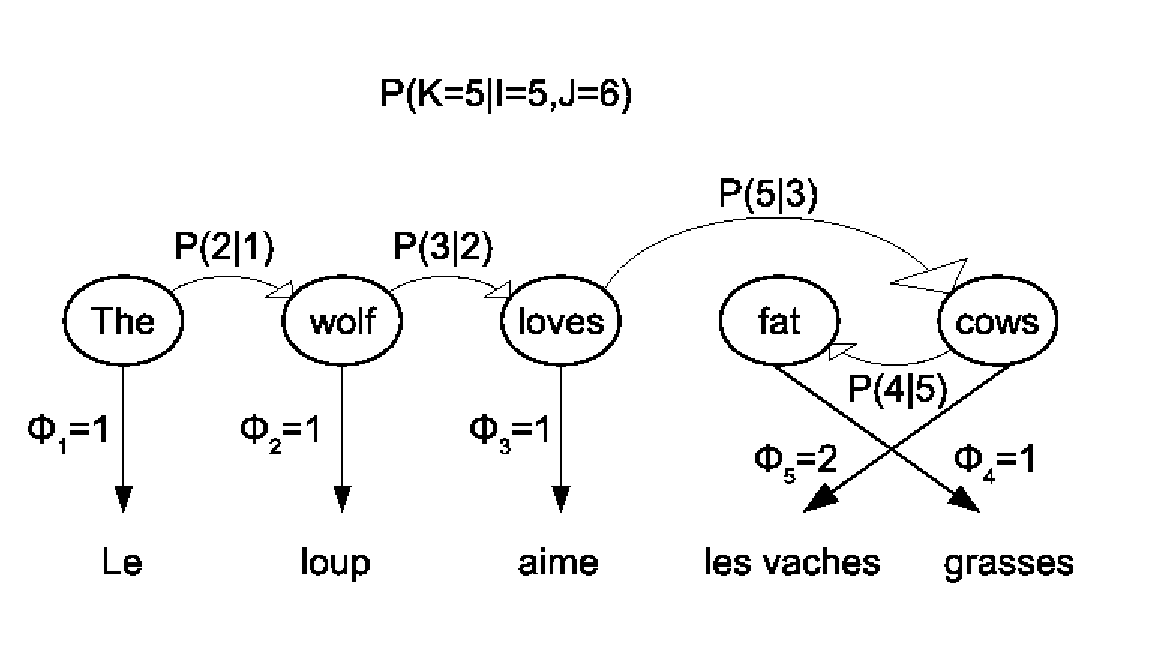
\includegraphics[scale=0.5]{figures/wordtophrase2.eps}
%  \end{center}
%  \caption{Illustrative example of an HMM word-to-phrase alignment model. The adjective noun sequence ``fat cows'' is
%    reordered into the noun adjective sequence ``vaches grasses''. The word ``cows'' has fertility 2 as it is translated
%    into the target phrase ``les vaches''.}
%  \label{fig:wordtophrase}
%\end{figure}
\begin{figure}
  \begin{center}
  \begin{tikzpicture} [node distance = 3cm, text height=1.5ex, text depth = .25ex, auto]
    % place nodes
    \node (the) {The};
    \node [right of = the] (wolf) {wolf};
    \node [right of = wolf] (loves) {loves};
    \node [right of = loves] (fat) {fat};
    \node [right of = fat] (cows) {cows};
    \node [above of = loves] (chooseSeg) {$p(K = 5 \mid I = 5, J = 6)$};
    
    \node [below of = the] (le) {Le};
    \node [below of = wolf] (loup) {loup};
    \node [below of = loves] (aime) {aime};
    \node [below of = fat] (lesVaches) {les vaches};
    \node [below of = cows] (grasses) {grasses};

    % draw edges
    \draw [->] (the) to node {$\phi_1 = 1$} (le);
    \draw [->] (wolf) to node {$\phi_2 = 1$} (loup);
    \draw [->] (loves) to node {$\phi_3 = 1$} (aime);
    \draw [->] (fat) to node [right, xshift = 1.5em, yshift = -1em] {$\phi_5 = 1$} (grasses);
    \draw [->] (cows) to node [left, xshift = -1.5em, yshift = -1em] {$\phi_4 = 2$} (lesVaches);

    \draw [->] (the) to [bend left = 45] node {$p(2 \mid 1)$} (wolf);
    \draw [->] (wolf) to [bend left = 45] node {$p(3 \mid 2)$} (loves);
    \draw [->] (loves) to [bend left = 45] node {$p(5 \mid 3)$} (cows);
    \draw [->] (cows) to [bend right = 45] node {$p(4 \mid 5)$} (fat);
  \end{tikzpicture}
  \end{center}
  \caption{Simplified generative story for an HMM word-to-phrase alignment model.
    Adapted from~\citep{deng-and-byrne:2008:ASLP}.
    The adjective noun sequence \emph{fat cows} is
    reordered into the noun adjective sequence \emph{vaches grasses}.
    The word \emph{cows} has fertility 2 as it is translated
    into the target phrase \emph{les vaches}.}
  \label{fig:wordtophrase}
\end{figure}

\subsection{Symmetrisation Heuristics}
\label{sec:symmetrisationHeuristics}

We have mentioned that the IBM and HMM alignment models
are not symmetric: they only allow a many-to-one mapping from
source words to target words.
In order to address this issue, one can train
alignment models in both source-to-target and target-to-source
directions, obtain Viterbi alignments from
both models and apply symmetrisation
strategies~\citep{och-tillmann-ney:1999:EMNLP,och-ney:2003:CL,koehn-och-marcu:2003:NAACL}.
\citet{och-tillmann-ney:1999:EMNLP} designed
a first symmetrisation heuristic that was later on dubbed
as the \emph{grow} heuristic. \citet{koehn-och-marcu:2003:NAACL}
later extend the \emph{grow} heuristic into
the \emph{grow-diag} and \emph{grow-diag-final} heuristics
and examine the impact on translation
performance for each heuristic.

Alignments from source to target (i.e. the alignment is
a function from source positions to target positions)
and target to source are denoted
$\bm{a}_{f2e}$ and $\bm{a}_{e2f}$ respectively.
Let us consider a sentence pair $(\bm{f}, \bm{e})$, and
source-to-target and target-to-source Viterbi alignments
$\bm{a}_{f2e}$ and $\bm{a}_{e2f}$.
The \emph{intersection} and \emph{union} heuristics
are defined as follows:
%
\begin{itemize}
  \item \emph{intersection}: $\bm{a} = \bm{a}_{e2f} \cap \bm{a}_{f2e}$
  \item \emph{union}: $\bm{a} = \bm{a}_{e2f} \cup \bm{a}_{f2e}$
\end{itemize}
%
The \emph{intersection} heuristics typically produces high precision alignments
while the \emph{union} heuristics typically produces high recall alignments.
We now present the \emph{grow} heuristic and its variants, which are based
on the initial \emph{intersection} and \emph{union} heuristics.
The \emph{grow} heuristic algorithm is presented in
\autoref{alg:growHeuristic}. The input is a sentence
pair $(f_1^J, e_1^I)$, a source-to-target
alignment $\bm{a}_{f2e}$ and a target-to-source alignment
$\bm{a}_{e2f}$. The resulting alignment $\bm{a}$ is initialized
with the
intersection (\hyperlink{alg:line:initGrow}{line \ref{alg:line:initGrow}}).
Then alignment links that are in the union and that are neighbours of already existing
alignment links (\hyperlink{alg:line:neighbours}{line \ref{alg:line:neighbours}})
are considered. If the source or the target word is not already
aligned (\hyperlink{alg:line:notAlreadyAligned}{line \ref{alg:line:notAlreadyAligned}}),
then the link is added to the resulting
alignment (\hyperlink{alg:line:addLink}{line \ref{alg:line:addLink}}).
This is repeated until no more links are added.
%
\begin{figure}
  %\begin{footnotesize}
  \begin{algorithmic}[1]
    \Function{Grow}{$f_1^J, e_1^J, \bm{a}_{f2e}, \bm{a}_{e2f}$}
      \State{$\bm{a} \gets \bm{a}_{f2e} \cap \bm{a}_{e2f}$} \hypertarget{alg:line:initGrow}{} \label{alg:line:initGrow}
      \While{\textbf{true}}
        \State{added $\gets$ \textbf{false}}
        \For{$i \in [1, I]$}
          \For{$j \in [1, J]$}
            \If{$(j, i) \in \bm{a}$}
            \For{$(k, l) \in $ \Call{Neighbours}{$(j,i)$} $\cap (\bm{a}_{f2e} \cup \bm{a}_{e2f})$} \hypertarget{alg:line:neighbours}{} \label{alg:line:neighbours}
              \If{$k$ not aligned in $\bm{a}$ \textbf{or} $l$ not aligned in $\bm{a}$} \hypertarget{alg:line:notAlreadyAligned}{} \label{alg:line:notAlreadyAligned}
                \State{$\bm{a} \gets \bm{a} \cup (k, l)$} \hypertarget{alg:line:addLink}{} \label{alg:line:addLink}
                \State{added $\gets$ \textbf{true}}
              \EndIf
            \EndFor
            \EndIf
          \EndFor
        \EndFor
        \If{not added} 
          \State{\textbf{break}}
        \EndIf
      \EndWhile
      \State{\Return $\bm{a}$}
    \EndFunction
  \end{algorithmic}
  %\end{footnotesize}
  \caption{Algorithm for the \emph{grow} symmetrisation heuristic.
    The alignment is initialized from the intersection and alignment links
    that are neighbours to existing alignment links are iteratively added if the source
    or the target is not already aligned.}
  \label{alg:growHeuristic}
\end{figure}

In the \emph{grow} heuristic, neighbours are defined as horizontal or
vertical neighbours. If diagonal neighbours are also considered, then
the heuristic becomes \emph{grow-diag}. The \emph{grow} heuristic
also has an optional step called \emph{final}. Alignment
links in the union where the source or the target is not already
aligned can also be added to the resulting alignment. If only links
in the union where the source \emph{and} the target are not already
aligned are considered for the \emph{final} procedure, then
the optional step is called \emph{final-and}.

Symmetrisation heuristics have been shown to be beneficial for
alignments both in terms of alignment quality as measured
by comparing automatic alignments to human alignments and
in translation quality when alignments are used as an
intermediate step in the translation pipeline.

%
%Symmetrised alignments have be shown to produce better translation results than
%unidirectional alignments. However, we find in one of our experiments that this
%is not always the case (see \autoref{sec:extractionFromPosteriorsSymmetrising}).

% This should review phrase based SMT.
% Why: the gyro decoder is like a phrase based SMT decoder.

% phrase based extraction + stack base decoding

\section{Log-Linear Model of Machine Translation}
\label{sec:loglinearModel}

%notes on adam berger paper
%model conditional prob
%p(y | x): x is phrase containing word "in", y is translation of "in"
%collect stats ptilda(x, y)
%binary feature: f(x, y) = 1 if y = en and April follows in
%expected value of f: ptilda(f) = sum_x,y ptilda(x,y) f(x,y)
%p(f) = sum_x,y ptilda(x) p(y | x) f(x,y)
%constraint: p(f) = ptilda(f)
%max entropy principle: choose p that satisfies the constraints
%and that maximizes entropy
%H(p) = -sum_x,y ptilda(x) p(y|x) log p(y|x)
%use Lagrange multiplier and Kuhn Tucker theorem to find that the solution
%is p(y|x) propto exp(\sum lambda_i f_i(x,y)). find lambda by max dual problem.
%also: p that satisfies constr and max entropy is also the
%p in the parametric family ... that maximizes likelihood of training sample.
%application to Candide.
%use max entropy modelling to predict translation of word in context.
%use max entropy modelling to predict word order.
%use max entropy modelling to segment.
%context dependent translation:
%first viterbi align training. then create events (x,y) (6 words
%surrounding in)
%incorporate this context dep translation into general translation model.

As we have seen in \autoref{sec:sourceChannelModel}, SMT was historically
framed as a source-channel model. As an alternative,
\citet{berger-dellapietra-dellapietra:1996:CL} introduce maximum entropy
models for natural language processing. In maximum entropy modelling, we
wish to estimate a conditional probability $p(\bm{y} \mid \bm{x})$.
Given a training sample, various feature functions deemed to be relevant
are picked. We then constrain $p$ such that the expected value of each
feature function $f$ with respect to the empirical distribution is equal
to the expected value of $f$ with respect to the model $p$. Finally, $p$
is chosen among all models that satisfy the constraints defined by the
features and such that its entropy is maximum.
\citet{berger-dellapietra-dellapietra:1996:CL} show how a maximum entropy
model can be parameterized as an exponential, or log-linear model. They
apply this model to three machine translation related tasks. First, they
use a maximum entropy model to predict the translation of a word using
the context for that word. Then, they use a maximum entropy model to
predict the target language word order. Finally, they apply maximum
entropy modelling in order to predict the source sentence segmentation.

%notes och and ney 2002
%search done by the maximum approximation
%first present log linear model
%log linear model generalization of source channel model
%log linear model presented with additional alignment variable
%p(e_1^I, a_1^J | f_1^J) propto exp(sum_1^M lambda_m h_m(e_1^I, f_1^J, a_1^J))
%alignment template model
%p(f_1^J | e_1^I) = sum_{z_1^K, a_1^K} p(a_1^K | e_1^I) . p(z_1^K | a_1^K, e_1^I) . p(f_1^J | z_1^K, a_1^K, e_1^I)
%each component modeled with max entropy model

\citet{och-tillmann-ney:1999:EMNLP} notice that using an erroneous
version of the source-channel model, that is using the following equation:
%
\begin{equation}
  \bm{\hat{e}} = \argmax_{\bm{e}} p(\bm{e} \mid \bm{f}) \, p(\bm{e})
\end{equation}
%
give comparable performance with respect to using the correct
formulation of the source-channel model given in \autoref{eq:noisy}.
Then \citet{och-ney:2002:ACL} propose the following log-linear model extension:
%
\begin{align}
  \bm{\hat{e}} &= \argmax_{\bm{e}} p(\bm{e} \mid \bm{f}) \nonumber \\
               &= \argmax_{\bm{e}} \frac{\exp(\sum_{m=1}^M \lambda_m h_m(\bm{e}, \bm{f}))}{\sum_{\bm{e'}}\exp(\sum_{m=1}^M \lambda_m h_m(\bm{e'}, \bm{f}))} \nonumber \\
               &= \argmax_{\bm{e}} \exp(\sum_{m=1}^M \lambda_m h_m(\bm{e}, \bm{f})) \label{eq:loglinearModel}
\end{align}
%
where $h_m$ are called \emph{feature functions} and $\lambda_m$
are called \emph{feature weights}. The log-linear model is an extension
to the noisy channel model because it can be reduced to the original
noisy channel model with the following settings:
%
    \begin{itemize}
      \item $M = 2$
      \item $h_1(\bm{e}, \bm{f}) = \log (p(\bm{f}|\bm{e}))$
      \item $h_2(\bm{e}, \bm{f}) = \log (p(\bm{e}))$
      \item $\lambda_1 = \lambda_2 = 1$
    \end{itemize}
%
Log-linear models were originally trained with the maximum likelihood
criterion, which precisely makes them equivalent to maximum entropy
models~\citep{berger-dellapietra-dellapietra:1996:CL}. However,
more effective training techniques such as minimum error rate
training~\citep{och:2003:ACL} were introduced later on, that do
not require the computation of the normalization constant
(see \autoref{sec:mert}).
Thus, in practice, SMT models are effectively simply linear models, with the objective
function presented in \autoref{eq:linearModel}:
%
\begin{equation}
  \bm{\hat{e}} = \argmax_{\bm{e}} \sum_{m=1}^M \lambda_m h_m(\bm{e}, \bm{f})
  \label{eq:linearModel}
\end{equation}

%In practice, \citet{och-ney:2002:ACL} do not use \autoref{eq:loglinearModel}.
%They introduce several latent variables in a so called \emph{alignment template}
%approach. The translation model is defined in \autoref{eq:alignmentTemplate}:
%
%\begin{equation}
%  p(e_1^I \mid f_1^J) = \sum_{z_1^K, a_1^K} p(a_1^K \mid e_1^I) p(z_1^K \mid a_1^K, e_1^I) p(f_1^J \mid z_1^K, a_1^K, e_1^I)
%  \label{eq:alignmentTemplate}
%\end{equation}
%
% TODO check if it is "correct" to invert the notation in above equation wrt to original publication
%where the variables $z_1^K$ and $a_1^K$ are alignment templates and the alignment of alignment templates.
%Each term in \autoref{eq:alignmentTemplate} is modelled as a maximum entropy model and search
%is carried out using the maximum approximation defined in \autoref{eq:maxApproximation}:
%
% TODO finish this
%\begin{align}
%  \hat{e_1^I} &= \argmax_{z_1}
%  \label{eq:maxApproximation}
%\end{align}

% TODO talk about training methods: GIS vs MERT

\section{Phrase-Based Translation}
\label{sec:phraseBasedTranslation}

%notes on och et al 1999
%compare word based and phrase based
%e = argmax p(e) p(f|e)
%word based model: each source word (french) assigned exactly one target word (english)
%difficult to model context and also to translate compound words
%model two alignment levels: phrase level alignment between phrases and word level alignment between words within phrases
%word based approach: use an HMM
%p(f_1^J | e_1^I) = sum_{a_1^J} prod_j p(a_j | a_{j - 1}) p(f_j | e_{a_j})
%some restrictions are used (so called monotonicity): alignment jump between a_{j - 1} and a_j can only be 0, 1, 2.
%Q_{e'}(j, e): probability of best partial hypothesis (e_1^i, a_1^j) with e_i = e, e_{i - 1} = e' and a_j = i
%search: mapping j -> (a_j, e_{a_j})
%DP recursion:
%Q_e'(j, e) = p(f_j | e) . max {
%  p(0) . Q_e'(j - 1, e),
%  p(1) . max_e'' {p(e | e', e'') Q_e''(j - 1, e')},
%  p(2) . max_{e'', e'''} {p(e | e', e'') . p(e' | e'', e''') . Q_e'''(j - 1, e'')}
%  }
%optimal translation: max_e',e Q_e'(J, e) . p(\$ | e, e')
%extension to one-to-many alignment model.
%solution: reverse translation direction, then extend English vocab with multiple words, then redo standard training for original translation direction.
%alignment template approach
%problem with word based models: only allow one to many or many to one, or many to many but hacky solution
%model phrase to phrase is a way to model context.
%alignment template z: triple (Ftilda, Etilda, Atilda) alignment Atilda between source class sequence Ftilda and
%target class sequence Etilda.
%Atilda: matrix with binary values
%Atilda allows for many to many
%Ftilda and Etilda automatically trained bilingual classes
%use classes for better generalization
%alignment template applicable to sequence source words ftilda if
%alignment template classes and classes of source words are equal
%application of alignment template contraints the target words to have the right classes
%selection target words: p(etilda | z, ftilda)
%p(ftilda | (Ftilda, Etilda, Atilda), etilda) = delta(classes(etilda), Etilda) delta(classes(ftilda), Ftilda) prod_{j=1}^J (I???) p(f_j | Atilda, etilda)
%p(f_j | Atilda, etilda) = sum_{i = 0}^I p(i | j; Atilda) p(f_j | e_i)
%p(i | j, Atilda) = Atilda(i, j) / (sum_i Atilda(i, j))
%rien compris
%phrase level alignment
%decompose f_1^J and e_1^I into sequence of phrases
%f_1^J = ftilda_1^K
%assume that there is only one possible segmentation (possibly one of the differences between Och and Koehn)
%p(f_1^J | e_1^I) = p(ftilda_1^K | etilda_1^K)
%                 = sum_{atilda_1^K} p(atilda_1^K, ftilda_1^K | etilda_1^K)
%                 = sum_{atilda_1^K} p(atilda_1^K | etilda_1^K) p(ftilda_1^K | atilda_1^K, etilda_1^K)
%                 = sum_{atilda_1^K} prod_{k = 1}^K p(atilda_k | atilda_1^{k-1}, K) p(ftilda_k | etilda_{atilda_k})
%p(ftilda | etilda) = sum_z p(z| etilda) p(ftilda | z, etilda)
%training: s2t and t2s hmm without the max approximation
%get the viterbi alignments a_1^J and b_1^I
%use the grow diag symmetrisation heuristic.
%estimate bilingual word lexicon p(f|e): n_A(f, e) | n(e)
%train world classes
%extract consistent phrase pairs from alignment
%obtain n(z) of how often alignment template occurs in aligned corpus.
%relative freq estimate: p(z = (Ftilda, Etilda, Atilda) | etilda) = n(z) . delta(classes(etilda), Etilda) / n(classes(etilda))
%decoding search
%objective: argmax_{e_1^I} p(e_1^I p(e_1^I | f_1^J)) (wrong version of source channel model)
%use class-based 5g lm
%preprocessing before translation: filter alignment templates per source sentence, segment source sentence
%segmentation objective: argmax_{ftilda_1...ftilda_k = f_1^J} prod_{k=1}^K max_z p(z | ftilda_k)
%search: produce partial hypotheses with info: last target word, language model state,
%source coverage, last alignment template, position of last target word in alignment template
%instantiation (???), cost so far, backpointer
%integrate future cost because compare hypotheses that cover different parts of the input

%notes on och-ney 2004 (journal paper version of och et al. 1999)
%overview: align, extract, extracted phrases with alignment and word classes are
%called alignment templates
%log-linear model: hat{e_1^I} = argmax_{e_1^I} p(e_1^I | f_1^J)
%                             = argmax exp(sum_m=1^M lambda_m h_m(e_1^I, f_1^J))/Z
%parameters lambda trained with MLE (same as maximum entropy)
%or trained with MERT
%use latent variable
%p(e_1^I, a_1^J | f_1^J) = (1/Z) . exp(sum_1^M lambda_m h_m(e_1^I, f_1^J, a_1^J))
%description of word alignments etc.
%description of symmetrisation heuristics etc.
%symmetrized Viterbi alignments used to compute translation lexicon
%description of phrase-extract
%alignment templates: replace words with word classes and store
%alignment info for each phrase pair
%alignment template z = (F_1^J', E_1^I', Atilda)
%F_1^J' source class sequence
%E_1^I' target class sequence
%Atilda: alignment between source class seq and target class seq
%automatically train bilingual classes
%notation: etilda, ftilda target and source phrases
%p(z = (F_1^J', E_1^I', Atilda) | ftilda) = N(z) . delta(F_1^J', C(ftilda)) / N(C(ftilda%))
%remove alignment templates with prob less than 0.01
%limit on source phrase: between 4 and 7
%translation model
%f_1^J = ftilda_1^K
%e_1^I = etilda_1^K
%model described for a specific segmentation but in search
%optimal segmentation also searched for
%pi_1^K: permutation of the phrases, models phrase reordering
%etilda_k is translation of ftilda_{pi_k}
%alignment template between f_{pi_k} and e_k: z_k
%hidden variables in the model: pi_1^K, z_1^K
%use log-linear model, feature functions depend on source, target and hidden variables
%features
%alignment template selection
%h_AT(e_1^I, f_1^J, pi_1^K, z_1^K) = log prod_1^K p(z_k | f_{j_{pi_k - 1} + 1}^{j_{pi_k}%})
%h_WRD(e_1^I, f_1^J, pi_1^K, z_1^K) = log prod_1^I p(e_i | {f_j, (i,j) in A}, E_i)
%p(e_i | {f_j, (i,j) in A}, E_i)
%etc etc. hyper complique
%h_AL phrase alignment (reordering model)
%h_AL(e_1^I, f_1^J, pi_1^K, z_1^K) = sum_{k=1}^{K+1} |j_{pi_k - 1} - j_{pi_{k - 1}}
%3gram lm + 5g class based lm
%training: blabla
%search
%breadth-first search with pruning: beam search
%search objective:
%hat{e_1^I} = argmax_{e_1^I} sum_{pi_1^K, z_1^K} p(e_1^I, z_1^K, pi_1^K | f_1^J)
%           ~~ argmax_{e_1^I, pi_1^K, z_1^K} p(e_1^I, z_1^K, pi_1^K | f_1^J)
%           = argmax_{e_1^I, pi_1^K, z_1^K} sum_{m = 1}^M lambda_m h_m(e_1^I, f_1^J, pi_%1^K, z_1^K)
%use the max approximation
%structure of search space
%generate hypothesis left to right on the target
%preprocessing step: first determine all source phrases that match an alignment template
%unknown words carried over
%use 5-best target words for each target class according to some criterion
%use hypothesis recombination
%pruning done for hypotheses that cover the same number of source words
%future cost estimation
%rien compris
%exps etc. etc.

%notes on phrase-based mt by koehn's book
%EM training of phrase-based models: NO
%Extensions to the Reordering Model
%zh-en, ar-en, fr-en in contrast to de-en or jp-en
%lexicalized reordering
%reordering model p_o predicts orientation m,s,d given phrase pair f,e:
%p_o(orientation | f, e)
%extract each phrase pair with orientation type p_o(orientation | f, e) = count(orientation, e, f) / sum_o count(o, e, f)
%to be smoothed with prior p_o(orientation)
%phrase translation as classification: use max ent model to model context
%use phrase penalty to model source segmentation
%use word penalty to model length
%lexical weighting a la koehn
%used as smoothing for translation model
%lex(e|f, a) = prod_{i = 1}^length(e) (1/|{j | (i,j) in a}|) sum_{j | (i,j) in a} w(e_i | f_j)
%if english word unaligned, use the NULL word on the f side
%w estimated with rel freq from aligned corpus.
%use both lex(e|f,a) and lex(f|e,a)
%log linear model: TODO find out what's the objective in moses/koehn2003
%phrase-extract etc. etc.
%source channel phrase-based model:
%e = argmax p(f|e) p(e)
%  = argmax prod_i p(f_i | e_i) d(start_i - end_{i - 1} -1)
%justification: segmentations are equally likely, max approximation ??
%d(x) propto alpha^|x|

%notes on phrase-based mt decoding by koehn's book
%description of hypothesis expansion
%computational complexity: NP complete/hard
%hypothesis recombination
%simple example: [it] [is] vs. [it is]
%more complicated example: [he] [does not] vs. [it] [does not]
%note: instead of deleting the hyp, we still keep pointer
%so that we can output n-best
%stack decoding
%stack <-> number of foreign words translated
%problem: some hyps in a stack cover different regions of the input
%histogram pruning and threshold pruning
%reordering limit in search
%future cost or outside cost or rest cost
%cost of translation option: translation cost easy,
%language model cost approximated by lm without context,
%reordering model ignored
%for each translation option, compute the ``cost without context''
%then estimate the cheapest cost for translating any span in the
%input using DP
%use future cost in search: add the cost of the remaining (gappy) span
%to the partial cost

%notes on koehn et al 2003
%"Note that phrase translation with a lexical weight is a
%special case of the alignment template model [Och et al.,
%1999] with one word class for each word."

So far, we have presented two modelling approaches to machine translation:
the original source-channel model and the current log-linear model. We also
have presented word alignment models, which were introduced within the source-channel
model framework and which are instances of word-based models.

% TODO motivation for phrase based: word based a:[1,J]->[1,I] so many to one mapping only
In the phrase-based translation paradigm, the minimal unit of translation consists
of phrases. Phrases are sequences of consecutive words, that need not be syntactically
or semantically motivated.
Benefits of phrase-based models include:
%
\begin{itemize}
  \item effectively disambiguating the translation of a word in a certain local context;
  \item effective local reordering such as the adjective-noun inversion from French to English;
  \item effective translation of multi-word expressions.
\end{itemize}
%
Phrase-based models
currently achieve state-of-the-art performance for
certain language pairs that do not involve much reordering
such as French-English. They can be defined
in the source-channel model framework (see \autoref{sec:sourceChannelModel}) or
the log-linear model framework (see \autoref{sec:loglinearModel}).
Because the source-channel model is rarely used anymore and because it is
a special case of a log-linear model, we will focus our presentation
on the log-linear model.

There are different variations on the phrase-based translation paradigm.
We will focus on two popular approaches, namely the alignment template
model~\citep{och-tillmann-ney:1999:EMNLP,och-ney:2004:CL} and the phrase-based
model~\citep{koehn-och-marcu:2003:NAACL,koehn:2010:book}.

\subsection{Alignment Template Model}

The alignment template model uses the log-linear model presented
in \autoref{eq:loglinearModel} as a starting point and repeated in
\autoref{eq:loglinearModelRepeated}:
%
\begin{equation}
  \bm{\hat{e}} = \argmax_{e_1^J} \exp(\sum_{m = 1}^M \lambda_m h_m(f_1^J, e_1^I))
  \label{eq:loglinearModelRepeated}
\end{equation}
%
In order to reduce the number of parameters, the two latent variables $\pi_1^K$
and $z_1^K$ are introduced. $z_1^K$ is a sequence of \emph{alignment templates}
while $\pi_1^K$ is a permutation of size $K$. An alignment template
is a triple $(\tilde{F}, \tilde{E}, \tilde{A})$ where $\tilde{F}$ is a
sequence of source word classes, $\tilde{E}$ is a sequence of target
word classes and $\tilde{A}$ is an alignment between $\tilde{F}$
and $\tilde{E}$. $\pi_1^K$ together with $z_1^K$ define
a source segmentation of $f_1^J$ into source phrases $\tilde{f}_1^K$,
a target segmentation of $e_1^I$ into target phrases $\tilde{e}_1^K$ and
a bijective mapping between source phrases and target phrases where
$\tilde{f}_{\pi_k}$ is mapped to $\tilde{e}_{k}$ for $k \in [1,K]$.
The alignment templates $z_1^K$ are constrained in such a way that
the alignment template classes match the word classes.
The alignment template translation model is summarized
in \autoref{fig:alignmentTemplateTranslationModel}.
%
\begin{figure}
  \begin{center}
    \begin{tikzpicture}[node distance = 1.5cm]
      % place nodes
      \node (f1) {$f_1$};
      \node (f2) [right of = f1] {$f_2$};
      \node (f3) [right of = f2] {$f_3$};
      \node (f4) [right of = f3] {$f_4$};
      \node (f5) [right of = f4] {$f_5$};
      \node (f6) [right of = f5] {$f_6$};
      \node (f7) [right of = f6] {$f_7$};

      \node (cf1) [below of = f1] {$\overline{f}_1$};
      \node (cf2) [below of = f2] {$\overline{f}_2$};
      \node (cf3) [below of = f3] {$\overline{f}_3$};
      \node (cf4) [below of = f4] {$\overline{f}_4$};
      \node (cf5) [below of = f5] {$\overline{f}_5$};
      \node (cf6) [below of = f6] {$\overline{f}_6$};
      \node (cf7) [below of = f7] {$\overline{f}_7$};

      \node (pf1) [below of = cf2] {$\widetilde{f}_1$};
      \node (pf2) [below of = cf3] {$\widetilde{f}_2$};
      \node (pf3) [below of = cf4] {$\widetilde{f}_3$};
      \node (pf4) [below of = cf5] {$\widetilde{f}_4$};

      \node (pe1) [below of = pf1] {$\widetilde{e}_1$};
      \node (pe2) [below of = pf2] {$\widetilde{e}_2$};
      \node (pe3) [below of = pf3] {$\widetilde{e}_3$};
      \node (pe4) [below of = pf4] {$\widetilde{e}_4$};

      \node (ce2) [below of = pe1] {$\overline{e}_2$};
      \node (ce1) [left of = ce2] {$\overline{e}_1$};
      \node (ce3) [below of = pe2] {$\overline{e}_3$};
      \node (ce4) [below of = pe3] {$\overline{e}_4$};
      \node (ce5) [below of = pe4] {$\overline{e}_5$};
      \node (ce6) [right of = ce5] {$\overline{e}_6$};

      \node (e1) [below of = ce1] {$e_1$};
      \node (e2) [below of = ce2] {$e_2$};
      \node (e3) [below of = ce3] {$e_3$};
      \node (e4) [below of = ce4] {$e_4$};
      \node (e5) [below of = ce5] {$e_5$};
      \node (e6) [below of = ce6] {$e_6$};
      % draw edges
      \draw [->] (f1) -- (cf1);
      \draw [->] (f2) -- (cf2);
      \draw [->] (f3) -- (cf3);
      \draw [->] (f4) -- (cf4);
      \draw [->] (f5) -- (cf5);
      \draw [->] (f6) -- (cf6);
      \draw [->] (f7) -- (cf7);

      \draw [->] (cf1) -- (pf1);
      \draw [->] (cf2) -- (pf1);
      \draw [->] (cf3) -- (pf2);
      \draw [->] (cf4) -- (pf3);
      \draw [->] (cf5) -- (pf4);
      \draw [->] (cf6) -- (pf4);
      \draw [->] (cf7) -- (pf4);

%      \draw[->] (P) to node {$\pi_{j}$} (B);

      \draw [->] (pf1) to node[left, xshift = -0.5em, yshift = 0.5em]{$z_1$} (pe2);
      \draw [->] (pf2) to node[right, xshift = 0.5em, yshift = 0.5em]{$z_2$} (pe1);
      \draw [->] (pf3) to node[left, xshift = -0.5em, yshift = 0.5em]{$z_3$} (pe4);
      \draw [->] (pf4) to node[right, xshift = 0.5em, yshift = 0.5em]{$z_4$} (pe3);

      \draw [->] (pe1) -- (ce1);
      \draw [->] (pe1) -- (ce2);
      \draw [->] (pe2) -- (ce3);
      \draw [->] (pe3) -- (ce4);
      \draw [->] (pe3) -- (ce5);
      \draw [->] (pe4) -- (ce6);

      \draw [->] (ce1) -- (e1);
      \draw [->] (ce2) -- (e2);
      \draw [->] (ce3) -- (e3);
      \draw [->] (ce4) -- (e4);
      \draw [->] (ce5) -- (e5);
      \draw [->] (ce6) -- (e6);
    \end{tikzpicture}
  \end{center}
  \caption{Alignment template translation process.
    Adapted from~\citep{och-ney:2004:CL}. The source word
  sequence $f_1^7$ is first transformed into a source class
  sequence $\overline{f}_1^7$. The source classes are then segmented
  into source phrases $\widetilde{f}_1^4$. The source phrases are then
  reordered and aligned to target phrases $\widetilde{e}_1^4$.
  For example, the source phrase $\widetilde{f}_1$ is aligned to
  the target phrase $\widetilde{e}_2$ through $z_1$.
  This means that the permutation $\pi_1^4$
  has value $\pi_2 = 1$. This also means that $z_1$
  define a word alignment between the source words $f_1$ and $f_2$
  and the target word $e_3$. Finally, the target
  phrases $\widetilde{e}_1^4$, which encode the target class sequence
  $\overline{e}_1^6$ generate the target word sequence $e_1^6$.}
  \label{fig:alignmentTemplateTranslationModel}
\end{figure}

Using the max approximation and making the feature
functions depend on the hidden variables, the translation model
can be rewritten in \autoref{eq:alignmentTemplateModel}:
%
\begin{equation}
  \bm{\hat{e}} = \argmax_{e_1^J, z_1^K, \pi_1^K} \exp(\sum_{m = 1}^M \lambda_m h_m(f_1^J, e_1^I, \pi_1^K, z_1^K))
  \label{eq:alignmentTemplateModel}
\end{equation}
%

% lexical feature in alignment template model
% symmetrized Viterbi alignments are used to compute a translation lexicon with relative frequency
% pi_1^K, z_1^K define an alignment between source and target: alignment A
% e_i has class E_i
% h_wrd(e_1^I, f_1^J, pi_1^K, z_1^K) = log prod_i=1^I p(e_i | {f_j | (i,j) in A}, E_i)
% p(e_i | {f_j | (i,j) in A}, E_i) = sum_{j | (i,j) in A} p(e_i | f_j) / |{j, (i,j) in A}| . delta(C(e_i), E_i)

\subsection{Phrase-Based Model}

The phrase-based model is similar to the alignment template
model but does not make use of source and target word classes.
Again, we use the latent variables $\pi_1^K$ and $z_1^K$.
This time, $z_k$ is defined as a triple $(\tilde{f}, \tilde{e}, \tilde{A})$
where $\tilde{f}$ is a sequence of source words, $\tilde{e}$ is a sequence
of target words and $\tilde{A}$ is an alignment between $\tilde{f}$ and $\tilde{e}$.
The reason for using the alignment information between phrase pairs is to be able
to compute the lexical feature (see \autoref{sec:features}).
Because the lexical feature can be computed
by other means than this alignment
information (see again \autoref{sec:features}), it is also possible to simply
define $z_k$ as a phrase pair.

We have presented two variants of the phrase-based model. We will now
describe how to obtain the phrase pairs used for the latent variable $z$.

\subsection{Phrase Pair Extraction}
\label{sec:phrasextract}

A preliminary step to phrase pair extraction
is to obtain word aligned parallel text.
One possibility is to train source-to-target and
target-to-source word alignment models, obtain
Viterbi alignments in both directions and
apply symmetrisation heuristics, as described
in \autoref{sec:symmetrisationHeuristics}.
Then phrase pairs are extracted from each
word aligned sentence pair.

Let us consider a sentence pair $(\bm{f},\bm{e})$ and an alignment $\bm{a}$.
We extract all phrase pairs that are {\em consistent} with the alignment.
This means that we extract all phrase pairs $(f_{j_1}^{j_2},e_{i_1}^{i_2})$ that
satisfy \autoref{eq:consistent} and \autoref{eq:atLeastOneLink}:
%
\begin{align}
  & \forall (j, i) \in \bm{a}, (j \in [j_1, j_2] \Leftrightarrow i \in [i_1,i_2]) \label{eq:consistent} \\
  & [j_1, j_2] \times [i_1, i_2] \cap \bm{a} \neq \emptyset \label{eq:atLeastOneLink}
\end{align}
%
\autoref{eq:consistent} requires that no alignment link be between a word
inside the phrase pair and a word outside the phrase pair.
\autoref{eq:atLeastOneLink} requires that there be at least one alignment link
between a source word in the source phrase and a target word in the target phrase.
For example, in \autoref{fig:ruleextract}, the phrase pair
$\langle$\emph{El mundo}, \emph{The world}$\rangle$ is extracted while the
phrase pair $\langle$\emph{es grande}, \emph{big}$\rangle$ is not
because the word \emph{es} (\emph{is}) is aligned
outside the phrase pair. Note that the consistency constraint
sometimes refers to only \autoref{eq:consistent} rather
than both \autoref{eq:consistent} and \autoref{eq:atLeastOneLink}.
%
\begin{figure}
  \begin{center}
    \begin{tikzpicture} [node distance = 2cm, text height=1.5ex, text depth=.25ex]
      % place nodes
      \node (El) {El};
      \node [right of = El] (mundo) {mundo};
      \node [right of = mundo] (es) {es};
      \node [right of = es] (grande) {grande};
      \node [below of = El] (The) {The};
      \node [right of = The] (world) {world};
      \node [right of = world] (is) {is};
      \node [right of = is] (big) {big};
      % draw edges
      \draw (El) -- (The);
      \draw (mundo) -- (world);
      \draw (es) -- (is) coordinate[midway](middleEsIs);
      \draw (grande) -- (big);
      % draw blocks around nodes to indicate rules
      %\node [draw=green, fit= (mundo) (world), rounded corners=1mm] {};
      \node [draw=green, fit= (El) (mundo) (The) (world), inner sep=1em, rounded corners=1mm] {};
      \draw [red, rounded corners=1mm] ($(es) + (-0.7,0.3)$) -- ($(big) + (0.7,-1.1)$) -- ($(grande) + (0.7,0.3)$) -- cycle;
      \node [ellipse, draw=red, minimum height = 4em, fit= (middleEsIs)] {};
    \end{tikzpicture}
  \end{center}
  \caption{Rule extraction for a sentence pair.
    For example, the phrase (El mundo, The world) is extracted.
    The phrase pair (es grande, big) is not extracted because it is
    not consistent with the alignment.}
  \label{fig:ruleextract}
\end{figure}
    
\subsection{Phrase-Based Decoding}
\label{sec:phraseBasedDecoding}

%notes on knight 1999 NP complete
%blabla on cryptograph and pos tagging
%machine translation
%v total English words
%bigram source model with v^2 parameters
%substitution/permutation channel models
%parallel corpus (sentence length <= m)
%monolingual french (???) sentence (length <= m)
%e_i has fertility phi_i: parameter n(phi | e)
%french words produced according to s(f|e) and permuted according to d(j|i,m,l)
%model 1 EM training
%collect estimate epsilon(m | l) from data
%set s(f|e) uniform initially
%basically, decoding with M1 is NP-complete
%reduction from hamilton circuit

We have introduced two types of phrase-based
models and described a technique to extract
phrase-pairs, which are an essential component
of these models. We will now describe the decoding
process, which is an effective means to obtain
the optimal translation of a source sentence.

We first describe a naive strategy for decoding, in order
to motivate the need for a more efficient decoder.
A naive decoder may follow the following steps, given
a source sentence $\bm{f}$ of length $J$ to be translated:
%
\begin{itemize}
  \item Consider all possible segmentations of $\bm{f}$ into source phrases. There are $2^{J - 1}$ such segmentations.
  \item For each segmentation, consider all possible permutations of the source phrases. For a segmentation of size $K$, there are $K!$ such permutations.
  \item For each permutation of the source phrases, consider all translations of each source phrase, and concatenate the target
    phrases according to the permutation. The source phrases translations are given by the phrase pairs extracted from the training
    data (see \autoref{sec:phrasextract}). If there are 10 translations per source phrase, we obtain
    $10^K$ possible translation (for the segmentation and permutation considered).
  \item Rank the translations by their score and pick the highest scoring translation.
\end{itemize}
%
We can see that the search space is too large for this naive
approach to be feasible.
We now present a better solution to the decoding process in phrase-based translation.
We will first introduce the translation process. Then, we will
describe how translation hypotheses are built incrementally.
We will then motivate the need for pruning and how pruning
is carried out. Finally, we will describe how future cost estimation
may reduce search errors.

\paragraph{Translation Process}

Given a source sentence, the translation process is to iteratively
pick a source phrase, translate that source phrase into a target phrase
and append the target phrase to the translation, until the source
sentence has been entirely covered by source phrases. While the process is not
complete, the concatenation of target phrases is called a
\emph{partial hypothesis}.

\paragraph{Hypothesis Expansion}

The decoding process starts from an initial empty partial hypothesis.
This empty partial hypothesis is extended by picking source phrases,
appending their translations to the empty hypothesis.
At this stage, we have obtained several partial hypotheses.
The partial hypotheses are repeatedly extended until
all source words have been covered.
Partial hypotheses are represented by states
that contain the information necessary to
compute the cost of an extension.
If we use an $n$-gram language model as a feature,
the state will encode the cost of the partial hypothesis
and the last $n - 1$ words of the partial hypothesis.

\paragraph{Hypothesis Recombination}
\label{sec:phraseBasedHypothesisRecombination}

When two partial hypotheses share the same $n - 1$
words, only the partial hypothesis with the lower
cost can lead to the best final hypothesis. Therefore,
the partial hypothesis with higher cost can be discarded, or
alternatively, it is possible to make these two partial
hypotheses share the same state for rescoring purposes.

\paragraph{Stack Based Decoding and Pruning}
\label{sec:phraseBasedPruning}

The decoding search space is very large
as seen above. Approximations
therefore need to be made for an effective search.
The partial hypotheses are grouped in \emph{stacks}
by the number of source words covered.
This allows pruning. Each time a hypothesis expansion produces a hypothesis that
belongs to a certain stack, that stack is pruned.
There are two types of pruning, histogram pruning and threshold
pruning. Histogram pruning enforces a maximum number
of partial hypotheses in each stack. Threshold pruning
examines the cost of the best partial hypothesis in a stack
and discards all partial hypotheses in that stack whose cost
is greater than the best cost plus a threshold.

\paragraph{Future Cost}
\label{sec:phraseBasedFutureCost}

Partial hypotheses that cover the same number of source
words are grouped together for pruning purposes. However,
their cost may not be directly comparable, for example
partial hypotheses that correspond to the translation of frequent
words in the source might have a smaller cost than partial hypotheses
that correspond to the translation of rare words in the source.
To address this issue, a future cost that represents how difficult it is
to translate the rest of the sentence is added to the model cost of each
partial hypothesis.

\section{Hierarchical Phrase-Based Translation}
\label{sec:hierarchicalPhraseBasedTranslation}

% TODO reread from here
% TODO rework outline:
% make a separate section on features after hiero section
% last subsection of hiero should be decoding with hifst

In the previous section, we have described the
phrase-based translation paradigm.
In this section, we present the
hierarchical phrase-based translation
model. This model relies on the synchronous
context free grammar formalism. Reordering
between source and target languages is modelled
by the grammar rather than by an \emph{ad hoc}
reordering model, although using both the grammar
and a reordering model may be
beneficial~\citep{huck-EtAl:2013:WMT}.
An alternative to hierarchical phrase-based
translation that also models discontinuous
phrases but does not use the same grammar
formalism has been introduced
recently~\citep{galley-manning:2010:NAACLHLT}.

\subsection{Introduction and Motivation}
\label{sec:hierintro}

Phrase-based models generally impose a limit on the size
of the phrase pairs extracted and, in decoding, phrases
are typically reordered within a certain limit.
These restrictions may be problematic for language pairs
such as German-English or Chinese-English that allow
arbitrary reordering in some instances.
Hierarchical phrase-based translation was introduced
in order to overcome the reordering limitations from
phrase-based models~\citep{chiang:2005:ACL,chiang:2007:CL}.
%A closely related formalism, inversion
%transduction grammars, was previously introduced~\citep{wu:1995:IJCAI,wu:1997:CL}. TODO put this somewhere else
For example, the Chinese sentence with English gloss
in \autoref{fig:exampleHiero} requires ``nested'' reordering~\citep{chiang:2007:CL}:
%
\begin{itemize}
  \item The phrase \emph{with North Korea have diplomatic relations} must be reordered into
    the phrase \emph{have diplomatic relations with North Korea}.
  \item The phrase \emph{few countries one of} must be reordered into the phrase \emph{one of (the) few countries}.
  \item After the two previous segments are reordered, \emph{have diplomatic relations with North Korea that one of the few countries} must be reordered into \emph{one of the few countries that have diplomatic relations with North Korea}.
\end{itemize}
%
\begin{CJK}{UTF8}{gbsn}
\begin{figure}
  \begin{center}
    \begin{footnotesize}
    \begin{tikzpicture} [node distance = 1.3cm]
      % place nodes
      \node (AustraliaZh) {澳洲};
      \node [right of = AustraliaZh](IsZh) {是};
      \node [right of = IsZh](WithZh) {与};
      \node [right of = WithZh](NorthKoreaZh) {北韩};
      \node [right of = NorthKoreaZh](HaveZh) {有};
      \node [right of = HaveZh](DiplomaticRelationsZh) {邦交};
      \node [right of = DiplomaticRelationsZh](ThatZh) {的};
      \node [right of = ThatZh](FewZh) {少数};
      \node [right of = FewZh](CountriesZh) {国家};
      \node [right of = CountriesZh](OneOfZh) {之一};

      \node [below of = AustraliaZh](AustraliaGloss) {Australia};
      \node [below of = IsZh](IsGloss) {is};
      \node [below of = WithZh](WithGloss) {with};
      \node [below of = NorthKoreaZh, align = left](NorthKoreaGloss) {North \\ Korea};
      \node [below of = HaveZh](HaveGloss) {have};
      \node [below of = DiplomaticRelationsZh, align = left](DiplomaticRelationsGloss) {diplomatic \\ relations};
      \node [below of = ThatZh](ThatGloss) {that};
      \node [below of = FewZh](FewGloss) {few};
      \node [below of = CountriesZh](CountriesGloss) {countries};
      \node [below of = OneOfZh, align = left](OneOfGloss) {one \\ of};

      \node [below = 4cm of AustraliaGloss](Australia) {Australia};
      \node [right of = Australia](Is) {is};
      \node [right of = Is, align = left](OneOf) {one \\ of};
      \node [right of = OneOf, align = left](Few) {the \\ few};
      \node [right of = Few](Countries) {countries};
      \node [right of = Countries](That) {that};
      \node [right of = That](Have) {have};
      \node [right of = Have, align = left](DiplomaticRelations) {diplomatic \\ relations};
      \node [right of = DiplomaticRelations](With) {with};
      \node [right of = With, align = left](NorthKorea) {North \\ Korea};

      % draw edges
      \draw (AustraliaGloss) -- (Australia);
      \draw (IsGloss) -- (Is);
      \draw (WithGloss) -- (With);
      \draw (NorthKoreaGloss) -- (NorthKorea);
      \draw (HaveGloss) -- (Have);
      \draw (DiplomaticRelationsGloss) -- (DiplomaticRelations);
      \draw (ThatGloss) -- (That);
      \draw (FewGloss) -- (Few);
      \draw (CountriesGloss) -- (Countries);
      \draw (OneOfGloss) -- (OneOf);
    \end{tikzpicture}
    \end{footnotesize}
  \end{center}
  \caption{Example of Chinese sentence that needs nested reordering in order to be translated into English.
  Adapted from \citep{chiang:2007:CL}.}
  \label{fig:exampleHiero}
\end{figure}
\end{CJK}  
%
Phrase-based systems can model this type of movement but
they need to use very long phrase pairs, which is
impractical because of data sparsity. On the other
hand, hierarchical phrase-based grammars do model this type of movement using
shorter phrase pairs but with more complex rules.

\subsection{Hierarchical Grammar}
\label{sec:hiergrammar}

\subsubsection{Hierarchical Grammar Definition}

A hierarchical phrase-based grammar, or hierarchical grammar, or Hiero grammar,
which is a particular instance of a synchronous context free
grammar~\citep{lewis-stearns:1968:JACM,aho:1969:JCSS}, is
a set of rewrite rules of the following type:
%
\begin{equation}
  X \rightarrow \langle \gamma, \alpha, \sim \rangle \nonumber
\end{equation}
%
where $X$ is a nonterminal, $\gamma$ and $\alpha$ are sequences of terminals and nonterminals and $\sim$ is an alignment
between nonterminals. Terminals that appear in $\gamma$ are words in the source language while terminals that appear in $\alpha$ are
words in the target language. Nonterminals are chosen from a finite set disjoint from the set of terminals. The alignment between nonterminals
indicates which nonterminals in the source and target languages correspond to each other. The alignment $\sim$ can be written with 
a set of matching indices.

\subsubsection{Types of Rules}

A rule may or may not contain any nonterminals.
A rule without nonterminals (on the right hand side) is
called a \emph{phrase-based rule}. A rule with nonterminals
is called a \emph{hierarchical rule}.
A hierarchical grammar also usually contains the following rules
called \emph{glue} rules:
%
\begin{align}
  S \rightarrow& \langle X, X \rangle \nonumber \\
  S \rightarrow& \langle S X, S X \rangle \nonumber
\end{align}
%
with $S$ the start symbol. The first glue rule is necessary to
be able to start a derivation.
The second glue rule allows concatenation of phrase-based or
hierarchical rules.

% TODO mention reordering and monotone rules
%When introducing hierarchical phrase-based translation, we mentioned
%that reordering between source and target language is modeled
%by the hierarchical grammar.
%This is achieved by so-called \emph{monotone}
%and \emph{reordering} rules. By definition, phrase-based
%rules are monotone.
%A hierarchical rule with one nonterminal only is monotone
%
%A hierarchical rule is monotone if it has a monotone
%alignment between nonterminals. For example, the
%rule $X \rightarrow \langle \text{\emph{Buenas tardes }} X, \text{\emph{ Good afternoon }} X \rangle$

\subsubsection{Hierarchical Grammar Example}

Let us consider for example the grammar
in \autoref{fig:exampleHieroGrammar} where each rewrite rule is given a name $R_i$.
%
\begin{figure}
\begin{CJK}{UTF8}{gbsn}
  \begin{align}
    R_1:&\; S \rightarrow \langle X, X \rangle \nonumber \\
    R_2:&\; S \rightarrow \langle S X, S X \rangle \nonumber \\
    R_3:&\; X \rightarrow \langle X_1 \mbox{ 的 } X_2, \mbox{ the } X_2 \mbox{ that } X_1 \rangle \nonumber \\
    R_4:&\; X \rightarrow \langle X \mbox{ 之一}, \mbox{ one of } X \rangle \nonumber \\
    R_5:&\; X \rightarrow \langle \mbox{与 } X_1 \mbox{ 有 } X_2, \mbox{ have } X_2 \mbox{ with } X_1 \rangle \nonumber \\
    R_6:&\; X \rightarrow \langle \mbox{澳洲}, \mbox{ Australia} \rangle \nonumber \\
    R_7:&\; X \rightarrow \langle \mbox{是}, \mbox{ is} \rangle \nonumber \\
    R_8:&\; X \rightarrow \langle \mbox{北韩}, \mbox{ North Korea} \rangle \nonumber \\
    R_9:&\; X \rightarrow \langle \mbox{邦交}, \mbox{ diplomatic relations} \rangle \nonumber \\
    R_{10}:&\; X \rightarrow \langle \mbox{少数 国家}, \mbox{ few countries} \rangle \nonumber
  \end{align}
  \caption{Example of hierarchical grammar.
    Adapted from~\citep{chiang:2007:CL}. With this grammar, it
    is possible to obtain a derivation for the sentence pair
    from \autoref{fig:exampleHiero}.
    The derivation is shown in \autoref{fig:exampleHieroDerivation}.}
  \label{fig:exampleHieroGrammar}
\end{CJK}
\end{figure}
%
With this grammar, it is possible to write a derivation, i.e.\ a sequence of rules,
that rewrites the start symbol $S$ into the sentence pair presented in
\autoref{sec:hierintro}~\citep{chiang:2007:CL}.
For example we can apply the derivation $R_2,R_2,R_1,R_6,R_7,R_4,R_3,R_{10},R_5,R_9,R_8$ as
in \autoref{fig:exampleHieroDerivation}.
%
\begin{figure}
\begin{CJK}{UTF8}{gbsn}
  \begin{footnotesize}
    \begin{align}
      S \rightarrow&\; \langle S X, S X \rangle \nonumber \\
      \rightarrow&\; \langle S X_1 X_2, S X_1 X_2 \rangle \nonumber \\
      \rightarrow&\; \langle X_1 X_2 X_3, X_1 X_2 X_3 \rangle \nonumber \\
      \rightarrow&\; \langle \mbox{澳洲 } X_2 X_3, \mbox{Australia } X_2 X_3 \rangle \nonumber \\
      \rightarrow&\; \langle \mbox{澳洲 是 } X_3, \mbox{Australia is } X_3 \rangle \nonumber \\
      \rightarrow&\; \langle \mbox{澳洲 是 } X \mbox{ 之一}, \mbox{Australia is one of } X \rangle \nonumber \\
      \rightarrow&\; \langle \mbox{澳洲 是 } X_1 \mbox{ 的 } X_2 \mbox{ zhiyi}, \mbox{Australia is one of the } X_2 \mbox{ that } X_1 \rangle \nonumber \\
      \rightarrow&\; \langle \mbox{澳洲 是 } X_1 \mbox{ 的 少数 国家 之一}, \mbox{Australia is one of the few countries that } X_1 \rangle \nonumber \\
      \rightarrow&\; \langle \mbox{澳洲 是 与 } X_1 \mbox{ 有 } X_2 \mbox{ 的 少数 国家 之一}, \nonumber \\
      &\;                    \mbox{Australia is one of the few countries that have } X_2 \mbox{ with } X_1 \rangle \nonumber \\
      \rightarrow&\; \langle \mbox{澳洲 是 与 } X_1 \mbox{ 有 邦交 的 少数 国家 之一}, \nonumber \\
      &\;                    \mbox{Australia is one of the few countries that have diplomatic relations with } X_1 \rangle \nonumber \\
      \rightarrow&\; \langle \mbox{澳洲 是 与 北韩 有 邦交 的 少数 国家 之一}, \nonumber \\ 
      &\;                    \mbox{Australia is one of the few countries that have diplomatic relations with North Korea} \rangle \nonumber
    \end{align}
  \end{footnotesize}
  \caption{Example of hierarchical grammar derivation.
    Adapted from~\citep{chiang:2007:CL}.
    A derivation is simply a sequence of rules that
    rewrite the start symbol $S$ into a sentence pair.
    This particular derivation produces the sentence pair from \autoref{fig:exampleHiero}.} % TODO better title, refer chiang and replace pinyin by chinese
  \label{fig:exampleHieroDerivation}
\end{CJK}
\end{figure}
%

\subsubsection{Constraints on Hierarchical Grammars}
\label{sec:constraintsOnHierarhicalGrammars}

The definition given for a hierarchical grammar is very general.
In practice, systems impose constraints on the types of rule the grammar contains
for efficiency reasons.
We first introduce the concept of rule
pattern~\citep{iglesias-degispert-banga-byrne:2009:EACL} in order
to describe these constraints in terms of patterns.
A rule pattern is simply a pair of regular expressions that match
the source and target sides of a hierarchical rule.
For example, the rule $X \rightarrow \langle \text{\emph{Buenas tardes }} X, \text{\emph{ Good afternoon }} X \rangle$
has a rule pattern $\langle \Sigma^+ X, \Psi^+ X \rangle$ where $\Sigma$ is the
source vocabulary and $\Psi$ is the target vocabulary.
For ease of notation, we use the notation $w$ for either $\Sigma^+$
or $\Psi^+$. Thus $w$ simply represents a sequence of terminals.
In our example, the pattern for the rule $ X \rightarrow \langle \text{\emph{Buenas tardes }} X, \text{\emph{ Good afternoon }} X \rangle$ is $\langle w X, w X \rangle$.
\citet{chiang:2007:CL} defines the following set of pattern-related constraints
that must be satisfied by the rules in a hierarchical grammar:
%
\begin{itemize}
  \item If a rule $X \rightarrow \langle \gamma, \alpha \rangle$ has a pattern $\langle w, w \rangle$, then $|\gamma| \leq 10$ and $|\alpha| \leq 10$.
  \item A rule $X \rightarrow \langle \gamma, \alpha \rangle$ must satisfy $|\gamma| \leq 5$.
  \item Rules have at most 2 nonterminals.
  \item The source side of a rule cannot have adjacent nonterminals.
    \citet{setiawan-resnik:2010:NAACL} relax this constraint.
    Note that the target side can still
    have adjacent nonterminals. %, for example see Section \ref{sec:emnlp10gramdef}.
  \end{itemize}
%
% TODO: missing constraints: boundary words, at least one alignment link
More fine-grained constraints can be defined on patterns.
For example, we use the configuration described
in \autoref{tab:patternconfig} for some of the translation experiments in this
thesis. This grammar was obtained following a greedy strategy of adding
in turn most beneficial patterns for Arabic-English translation.

  \begin{table}[htbp]
    \begin{center}
      \footnotesize
      \begin{tabular}{|r@{ , }l|c||r@{ , }l|c|} \hline 
        {\bf \SR[source]} & {\bf\TR[target]} & {\bf include} & {\bf \SR[source]} & {\bf\TR[target]} & {\bf include} \\ \hline
        \SR[$w~X$] & \TR[$w~X$] & \textbf{no}  & \SR[$X~w$] & \TR[$w~X$] & yes \\
        \SR[$w~X$] & \TR[$X~w$] & yes &  \SR[$X~w$] & \TR[$w~X~w$] & yes \\
        \SR[$w~X$] & \TR[$w~X~w$] & yes  & \SR[$X~w$] & \TR[$X~w$] & \textbf{no} \\
        \hline
        \SR[$w~X~w$] & \TR[$w~X$] & yes &  \SR[$w~X~w$] & \TR[$X~w$] & yes \\
        \SR[$w~X~w$] & \TR[$w~X~w$] & yes &  \multicolumn{2}{|c|}{} & \\
        \hline
        \SR[$X1~w~X2$] & \TR[$w~X1~w~X2$] & \textbf{no} &  \SR[$X2~w~X1$] & \TR[$w~X1~w~X2$] & yes \\
        \SR[$X1~w~X2$] & \TR[$w~X1~w~X2~w$] & \textbf{no} &  \SR[$X2~w~X1$] & \TR[$w~X1~w~X2~w$] & yes \\
        \SR[$X1~w~X2$] & \TR[$w~X1~X2$] & \textbf{no} & \SR[$X2~w~X1$] & \TR[$w~X1~X2$] & yes \\
        \SR[$X1~w~X2$] & \TR[$w~X1~X2~w$] & \textbf{no} & \SR[$X2~w~X1$] & \TR[$w~X1~X2~w$] & yes \\
        \SR[$X1~w~X2$] & \TR[$X1~w~X2$] & \textbf{no} & \SR[$X2~w~X1$] & \TR[$X1~w~X2$] & yes \\
        \SR[$X1~w~X2$] & \TR[$X1~w~X2~w$] & \textbf{no} & \SR[$X2~w~X1$] & \TR[$X1~w~X2~w$] & yes \\
        \SR[$X1~w~X2$] & \TR[$X1~X2~w$] & \textbf{no} & \SR[$X2~w~X1$] & \TR[$X1~X2~w$] & yes \\
        \hline
        \SR[$w~X1~w~X2$] & \TR[$w~X1~w~X2$] & \textbf{no} & \SR[$w~X2~w~X1$] & \TR[$w~X1~w~X2$] & yes \\
        \SR[$w~X1~w~X2$] & \TR[$w~X1~w~X2~w$] & yes & \SR[$w~X2~w~X1$] & \TR[$w~X1~w~X2~w$] & yes \\
        \SR[$w~X1~w~X2$] & \TR[$w~X1~X2$] & yes & \SR[$w~X2~w~X1$] & \TR[$w~X1~X2$] & yes \\
        \SR[$w~X1~w~X2$] & \TR[$w~X1~X2~w$] & yes & \SR[$w~X2~w~X1$] & \TR[$w~X1~X2~w$] & yes \\
        \SR[$w~X1~w~X2$] & \TR[$X1~w~X2$] & yes & \SR[$w~X2~w~X1$] & \TR[$X1~w~X2$] & yes \\
        \SR[$w~X1~w~X2$] & \TR[$X1~w~X2~w$] & yes & \SR[$w~X2~w~X1$] & \TR[$X1~w~X2~w$] & yes \\
        \SR[$w~X1~w~X2$] & \TR[$X1~X2~w$] & yes & \SR[$w~X2~w~X1$] & \TR[$X1~X2~w$] & yes \\
        \hline
        \SR[$X1~w~X2~w$] & \TR[$w~X1~w~X2$] & yes & \SR[$X2~w~X1~w$] & \TR[$w~X1~w~X2$] & yes \\
        \SR[$X1~w~X2~w$] & \TR[$w~X1~w~X2~w$] & yes & \SR[$X2~w~X1~w$] & \TR[$w~X1~w~X2~w$] & yes \\
        \SR[$X1~w~X2~w$] & \TR[$w~X1~X2$] & yes & \SR[$X2~w~X1~w$] & \TR[$w~X1~X2$] & yes \\
        \SR[$X1~w~X2~w$] & \TR[$w~X1~X2~w$] & yes & \SR[$X2~w~X1~w$] & \TR[$w~X1~X2~w$] & yes \\
        \SR[$X1~w~X2~w$] & \TR[$X1~w~X2$] & yes & \SR[$X2~w~X1~w$] & \TR[$X1~w~X2$] & yes \\
        \SR[$X1~w~X2~w$] & \TR[$X1~w~X2~w$] & \textbf{no} & \SR[$X2~w~X1~w$] & \TR[$X1~w~X2~w$] & yes \\
        \SR[$X1~w~X2~w$] & \TR[$X1~X2~w$] & yes & \SR[$X2~w~X1~w$] & \TR[$X1~X2~w$] & yes \\
        \hline
        \SR[$w~X1~w~X2~w$] & \TR[$w~X1~w~X2$] & \textbf{no} & \SR[$w~X2~w~X1~w$] & \TR[$w~X1~w~X2$] & yes \\
        \SR[$w~X1~w~X2~w$] & \TR[$w~X1~w~X2~w$] & \textbf{no} & \SR[$w~X2~w~X1~w$] & \TR[$w~X1~w~X2~w$] & yes \\
        \SR[$w~X1~w~X2~w$] & \TR[$w~X1~X2$] & \textbf{no} & \SR[$w~X2~w~X1~w$] & \TR[$w~X1~X2$] & yes \\
        \SR[$w~X1~w~X2~w$] & \TR[$w~X1~X2~w$] & \textbf{no} & \SR[$w~X2~w~X1~w$] & \TR[$w~X1~X2~w$] & yes \\
        \SR[$w~X1~w~X2~w$] & \TR[$X1~w~X2$] & \textbf{no} & \SR[$w~X2~w~X1~w$] & \TR[$X1~w~X2$] & yes \\
        \SR[$w~X1~w~X2~w$] & \TR[$X1~w~X2~w$] & \textbf{no} & \SR[$w~X2~w~X1~w$] & \TR[$X1~w~X2~w$] & yes \\
        \SR[$w~X1~w~X2~w$] & \TR[$X1~X2~w$] & \textbf{no} & \SR[$w~X2~w~X1~w$] & \TR[$X1~X2~w$] & yes \\
        \hline
      \end{tabular}
    \end{center}
    \caption{Rule patterns included in a baseline hierarchical grammar.}
    \label{tab:patternconfig}
  \end{table}
  
  Another restriction on hierarchical grammar is the amount of reordering allowed. \citet{degispert-iglesias-blackwood-banga-byrne:2010:CL} investigate the use
  of shallow-$N$ grammars that precisely control the depth of reordering in translation. We describe here 
  shallow-1 grammars~\citep{iglesias-degispert-banga-byrne:2009:EACL,degispert-iglesias-blackwood-banga-byrne:2010:CL} as
  they will be used for translation experiments in this thesis. Shallow-1 grammars
  allow only one level of reordering, they do not allow nested reordering as in the example presented in \autoref{sec:hierintro}.
  A shallow-1
  grammar is defined as follows:
%  
  \begin{align*}
    S &\rightarrow \langle X , X \rangle \\
    S &\rightarrow \langle S X , S X \rangle \\
    X &\rightarrow \langle \gamma_s , \alpha_s \rangle (\gamma_s, \alpha_s \in (T \cup \{V\})^{+}) \\
    X &\rightarrow \langle V , V \rangle \\
    V &\rightarrow \langle s , t \rangle (s \in T^{+}, t \in  T^{*})
  \end{align*}
%  
  where $S$ is the start symbol, $T$ is the set of terminals and $V$ is the set of nonterminals. There are two nonterminals
  apart from the start symbol: $X$ and $V$. The rule type $X \rightarrow \langle \gamma_s , \alpha_s \rangle$ corresponds
  to all hierarchical rules. It is possible to apply this type of rule only once. Indeed, the
  right hand side contains only one type of nonterminal, $V$, which can be rewritten only with a phrasal rule corresponding
  to the line $V \rightarrow \langle s , t \rangle$. Note that for rules of the type $V \rightarrow \langle s , t \rangle$, $t$ can be
  the empty word, thus these rules, called {\em deletion rules}, allow deletion on the target side. Shallow-1 grammar are used for language pairs that do not present
  much reordering. Shallow-1 grammars were previously shown to work as well as full hierarchical grammars
  for the Arabic-English language pair~\citep{iglesias-degispert-banga-byrne:2009:EACL} and for
  the Spanish-English language pair~\citep{iglesias-degispert-banga-byrne:2009:SEPLN}.
  In addition, shallow-1 grammars reduce the search space of the decoder greatly, resulting in a much faster decoding
  time, a reduced memory use and potentially less search errors.

  % TODO log linear model for hpbt

    \subsection{Log-linear Model for Hierarchical Phrase-Based Translation} \label{sec:loglinear}

    We now define in more detail the log-linear model for hierarchical translation, which usually makes a maximum (max) approximation.
    We follow the original description~\citep{chiang:2007:CL}.
    For a sentence pair $(\bm{f}, \bm{e})$, let us define $\mathcal{D}$ the set of possible derivations $D$ of this sentence pair under 
    a hierarchical grammar. We will use the following notation for a derivation $D$:
    
    \begin{itemize}
%      \item $T$, the structure of the tree (that is the tree $D$ without leaves)
      \item the foreign yield $\bm{f}$. We define $f(D) = \bm{f}$
      \item the English yield $\bm{e}$. We define $e(D) = \bm{e}$
    \end{itemize}

    %Let us define $d = (T,{\bf f})$, so that we have $D = (d,{\bf e})$. 
    We can now derive the log-linear model for hierarchical translation:

    \begin{eqnarray}
      \hat{{\bf e}} &=& \argmax_{\bm{e}} p(\bm{e} \mid \bm{f}) \nonumber \\
                    &=& \argmax_{\bm{e}} \sum_{D \in \mathcal{D}} p(D,\bm{e} \mid \bm{f}) \mbox{ (marginalisation)} \nonumber \\
                    %&=& \argmax_{e} \sum_{d} p(d,{\bf e}|{\bf f}) \mbox{ (simply because the event D,{\bf e} is the same as the event d,{\bf e}} \\
                    &=& \argmax_{\bm{e}} \argmax_{D \in \mathcal{D}} p(D,\bm{e} \mid \bm{f}) \mbox{ (max approximation)} \nonumber \\
                    &=& e(\argmax_{{\bf e},D \in \mathcal{D}} p(D,{\bf e}|{\bf f})) \nonumber \\
                    &=& e(\argmax_{D | f(D) = {\bf f}} p(D))
    \end{eqnarray}

    Thanks to the max approximation, the distribution over derivations instead of the distribution over English
    sentences is modelled log-linearly and we obtain finally the following decoding equation:
%
    \begin{equation} \label{eq:decoding}
      \hat{{\bf e}} = e(\argmax_{D | f(D) = {\bf f}} \exp(\sum_{m=1}^M \lambda_m h_m(D)))
    \end{equation}
%
    One of the features, the language model, plays a particular role. The language model feature can be written as:
%    
    \begin{equation}
      h_M(D) = p_{LM}(e(D))
    \end{equation}
    
    \noindent where $M$ is the index of the language model feature, $p_{LM}$ is the language model and $e(D)$ is the English
    yield of the derivation $D$. It is not possible to compute the language model using dynamic programming since
    the language model needs context in order to be computed, therefore the language model feature is typically
    computed after a parsing step. % TODO explain better. for this, reread chiang's paper and/or hifst paper(s)
    
    Note that Equation (\ref{eq:decoding}) is an approximation and that there have been attempts to perform marginalisation over the latent variable 
    $D$ while keeping the translation process tractable~\citep{blunsom-cohn-osborne:2008:ACL,degispert-iglesias-blackwood-banga-byrne:2010:CL}.

    %We now describe which features are used in our system, except for the language model which will be presented in Section \ref{lm}.

  \subsection{Rule Extraction} \label{sec:hierruleextract}

  We have so far given the definition of a hierarchical grammar and explained how it is used with statistical models.
  It is also necessary to extract an appropriate grammar, that is the rules it contains. The extraction
  is performed on a parallel corpus. The parallel corpus is first word-aligned, then
  rules are extracted from the alignment.

  We first extract phrase pairs as described in \autoref{sec:phrasextract}.
  For each extracted phrase pair $\langle f_{j_1}^{j_2}, e_{i_1}^{i_2} \rangle$,
  we define the following
  rule: $X \rightarrow \langle f_{j_1}^{j_2},e_{i_1}^{i_2} \rangle$.
  These rules are called {\em initial rules}.
      We extend the set of initial rules with the following recursion: given a rule  $X \rightarrow \langle \gamma, \alpha \rangle$
      and an initial rule $X \rightarrow \langle f_{j_1}^{j_2},e_{i_1}^{i_2} \rangle$ such that $\gamma = \gamma_1 f_{j_1}^{j_2} \gamma_2$
      and $\alpha = \alpha_1 e_{i_1}^{i_2} \alpha_2$, then extract the rule $X \rightarrow \langle \gamma_1 X \gamma_2, \alpha_1 X \alpha_2 \rangle$.
      Note that $\gamma_1$ or $\gamma_2$, but not both, can be the empty word, and similarly for $\alpha_1$ and $\alpha_2$.

%      \subsubsection{Glue Rules}
%
%      The following two rules are added in order to respectively be able to start a derivation and to add concatenation capabilities to the grammar, as
%      mentioned in Section \ref{sec:hierhiero}:
%
%      \begin{eqnarray}
%        S &\rightarrow& \langle X, X \rangle \nonumber\\
%        S &\rightarrow& \langle S X, S X \rangle
%      \end{eqnarray}
%
%      \subsubsection{Extraction in Practice}

%      In practice, initial rule extraction and hierarchical rule extraction
%      are not sequential steps and can be done simultaneously. For example, let us imagine we want to extract
%      hierarchical rules corresponding to the pattern $\langle wX, wX \rangle$. Then we loop over sequences of two consecutive source phrases
%      and over sequences of two consecutive target phrases and check that the phrase pairs (first source phrase, first target phrase) and
%      (second source phrase, second target phrase) are consistent with the alignment, and replace
%      the second phrase pair (second source phrase, second target phrase) by a nontermi%nal $X$.

\subsection{Features}
\label{sec:features}

    The following features are commonly used in log-linear models for machine translation:
%    
    \begin{itemize}
      \item Source-to-target and target-to-source translation models. As described above, the 
        translation process produces a derivation $D$. A derivation $D$ can be seen
        as a sequence of $n$ rules 
        $X \rightarrow \langle \alpha_1, \gamma_1 \rangle, ..., X \rightarrow \langle \alpha_n, \gamma_n \rangle$.
        Then the source-to-target translation model is simply $\prod_{i=1}^n p(\gamma_i|\alpha_i)$ where
        the $p(\gamma_i|\alpha_i)$ are typically estimated using relative frequency, based on the appearance 
        of phrasal and hierarchical rules in the parallel corpus
        %, which will be described in Section \ref{sec:hierextraction}.
        The target-to-source 
        translation model is symmetric.
      \item Source-to-target and target-to-source lexical translation model. Typically, the source-to-target lexical translation
        model $lx(f_1^J,e_1^I)$ is computed as following for a foreign sentence $f_1^J$ translated into the English sentence $e_1^I$:

        \begin{equation} \label{eq:lexfeature}
          lx(f_1^J,e_1^I) = \frac{1}{(I+1)^J}\prod_{j=1}^{J} \sum_{i=0}^{I} p_1(e_i|f_j)
        \end{equation}

        \noindent where $p_1$ is the word-to-word translation probability in IBM Model 1 and $e_0$ the null word. The target-to-source lexical translation model is symmetric. One reason to use lexical models in addition to translation models is that translation models are relatively sparse compared
        to lexical models, thus lexical models can smooth the translation models.

      \item Number of uses of the glue rule. This feature trades off monotonic translation versus reordering.
      \item Word insertion penalty. This feature controls the length of the output.
      \item Rule insertion penalty. This feature controls the number of derivations in decoding. Using many rules is closer to word-to-word
        translation while using few rules means that longer phrase pairs are used. This feature is similar to the phrase penalty in phrase-based
        statistical machine translation \cite{koehn-och-marcu:2003:NAACL}.
      \item Word deletion scale factor. This feature controls the number of times a deletion rule is applied.
      \item Rule count feature. This feature indicates 
        whether a rule occurs once, twice or more in the parallel data~\citep{bender:07}. Thus it indicates how reliable a rule is.
    \end{itemize}

    The feature weights are optimized using minimum error rate training \cite{och:2003:ACL} under the BLEU 
    score \cite{papineni-roukos-ward-zhu:2002:ACL}, which will be described
    in \autoref{sec:optimization}.
    %Minimum error rate training is described in more detail in Section \ref{sec:syscombmert}.

\section{Language Modelling}
\label{sec:languageModelling}

% This should review backoff and modified kneser-ney smoothing.
% Why: LM interpolation gains.

% outline: introduction, definition, smoothing strategies

We mentioned in Section \ref{sec:loglinear} that a language model was one of the features of
log-linear models for translation. This feature is critical as it helps to obtain a fluent
translation output. A language model is a probability distribution over word sequences. It can be used to assign
a probability to a sequence of words or to predict the word most likely to appear in a certain context.
Language models have applications in fields where the goal is to produce fluent output, such
as automatic speech recognition or machine translation.
$n$-gram language models are typically used because they are 
robust, can be easily trained on large amounts of data and model local grammatical relationships.
Since they do not model the language structure nor long distance relationships between words, work
has been conducted~\citep{shen-xu-weischedel:2008:ACL} to overcome this issue. % TODO move this or expand
We first review $n$-gram language models, then review different smoothing techniques, we finally
describe in more detail two smoothing techniques
that are used for experiments in this thesis: Kneser-Ney smoothing
and Stupid-Backoff smoothing.

\subsection{$n$-gram language models}
\label{sec:ngramLanguageModels}

For simplicity, let us first consider the case of a bigram language model.
Let us consider a vocabulary $V$ and the two special symbols \texttt{<s>} and \texttt{</s>}
corresponding respectively to the start-of-sentence symbol and the
end-of-sentence symbol. We define
$W = V \cup \{\text{\texttt{<s>}}, \text{\texttt{</s>}}\}$. Let us now define
the Markov chain $(X_i)_{i \in \mathbb{N}}$ with values in $W$ and transition
probability $p$. $p$ has the following properties:
%
\begin{itemize}
  \item $p(X_0 = \text{\texttt{<s>}}) = 1$: we always start a sentence with a start-of-sentence
    symbol.
  \item $p(X_{n + 1} = \text{\texttt{</s>}} \mid X_n = \text{\texttt{</s>}}) = 1$: once we reach the end of a
    sentence, we stay in the end-of-sentence state. This is because we do not
    consider infinite word sequences.
  \item $p(X_{n + 1} = \text{\texttt{<s>}} \mid X_n = \text{\texttt{<s>}}) = 0$: we cannot stay in the
    start-of-sentence state and have to transition to either a word or the
    end-of-sentence state.
\end{itemize}
% TODO maybe add a condition that p(w | v) < 1 to prevent prob mass to infinite
% sequences
%
A bigram model is defined by the conditional independence assumptions of the
Markov chain $(X_i)$ and the translation probability $p$. A bigram model will
therefore assign the probability $p(\bm{w})$ to a sequence of words
$\bm{w} = w_1...w_n$ in \autoref{eq:bigramProbability}:
%
\begin{equation}
  p(\bm{w}) = \prod_{i = 1}^{n+1} p(w_i \mid w_{i - 1})
  \label{eq:bigramProbability}
\end{equation}
%
with the convention $w_0 = \text{\texttt{<s>}}$ and $w_{n+1} = \text{\texttt{</s>}}$.

An $n$-gram language model can be defined similarly: this time the random
variables $X_i$ take values in $W^{n - 1}$ instead of $W$. An $n$-gram model % TODO maybe define properly instead of saying it's the same
will assign the probability $p(\bm{w})$ to a sequence of words
$\bm{w} = w_1...w_n$ in \autoref{eq:ngramProbability}:
%
\begin{equation}
  p({\bf w}) = \prod_{i=1}^{n + 1} p(w_i \mid w_{i-n+1}^{i-1})
  \label{eq:ngramProbability}
\end{equation}
%
with the same convention that $w_0 = \text{\texttt{<s>}}$
and $w_{n+1} = \text{\texttt{</s>}}$.
Parameters can be trained using maximum likelihood estimation, so the parameter
$p(w_i|w_{i-n+1}^{i-1})$ is computed in \autoref{eq:ngramMLE}.
%
\begin{equation}
  p(w_i|w_{i-n+1}^{i-1}) = \frac{c(w_{i-n+1}^{i})}{c(w_{i-n+1}^{i-1})}
  \label{eq:ngramMLE}
\end{equation}
%
where $c(.)$ counts the number of occurrences of a particular word sequence in
the training data. Maximum likelihood estimation assigns zero probability to
unseen events, therefore different smoothing strategies have been explored to
address this problem.

\subsection{Back-off and Interpolated Models}
\label{sec:backoffAndInterpolatedModels}

% TODO look at cutoffs

Smoothing strategies for language modelling make use of lower order
distributions either by backoff or interpolation. The general form of a backoff
model~\citep{chen-goodman:1998:harvard} is presented in \autoref{eq:backoffModel}:
%
\begin{equation}
  p_{\text{backoff}}(w_i \mid w_{i - n + 1}^{i - 1}) =
  \begin{cases}
    \alpha(w_i \mid w_{i - n + 1}^{i - 1}) & \text{if } c(w_{i - n + 1}^i) > 0 \\
    \gamma(w_{i - n + 1}^{i - 1}) p_{\text{backoff}}(w_i \mid w_{i - n + 2}^{i - 1}) & \text{if } c(w_{i - n + 1}^i) = 0
  \end{cases}
  \label{eq:backoffModel}
\end{equation}
%
The conditions $c(w_{i - n + 1}^i) > 0$ and $c(w_{i - n + 1}^i) = 0$
can be replaced by $c(w_{i - n + 1}^i) \geq \text{\emph{cutoff}}$ and
$c(w_{i - n + 1}^i) < \text{\emph{cutoff}}$ respectively when $n$-grams with
an occurrence less than the \emph{cutoff} threshold are ignored
in the training data.

The general form of an interpolated model~\citep{chen-goodman:1998:harvard} is
presented in \autoref{eq:interpolatedModel}:
%
\begin{equation}
  \begin{split}
    p_{\text{interpolate}}(w_i \mid w_{i - n + 1}^{i - 1}) = & \; \lambda_{w_{i - n + 1}^{i - 1}} p_{\text{ML}}(w_i \mid w_{i - n + 1}^{i - 1}) + \\
                                                             & \; (1 - \lambda_{w_{i - n + 1}^{i - 1}}) p_{\text{interpolate}}(w_i \mid w_{i - n + 2}^{i - 1})
  \end{split}
  \label{eq:interpolatedModel}
\end{equation}
%
where:
%
\begin{itemize}
  \item $p_{\text{ML}}$ is the maximum likelihood estimate.
  \item $\lambda_{w_{i - n + 1}^{i - 1}}$ is the interpolation parameter.
\end{itemize}
%
The difference between backoff and interpolated model is that interpolated
models make use of lower order distributions even when the $n$-gram counts are
greater than zero. However, an interpolated model can be written in the form
of a backoff model.
Let us define $\alpha(w_i \mid w_{i - n + 1}^{i - 1})$ in \autoref{eq:alphaForInterp}:
%
\begin{equation}
  \alpha(w_i \mid w_{i - n + 1}^{i - 1}) = p_{\text{interpolate}}(w_i \mid w_{i - n + 1}^{i - 1})
  \label{eq:alphaForInterp}
\end{equation}
%
and $\gamma(w_{i - n + 1}^{i - 1})$ in \autoref{eq:gammaForInterp}:
%
\begin{equation}
  \gamma(w_{i - n + 1}^{i - 1}) = 1 - \lambda_{w_{i - n + 1}^{i - 1}}
  \label{eq:gammaForInterp}
\end{equation}
%
We can see that by plugging in the definitions of
$\alpha(w_i \mid w_{i - n + 1}^{i - 1})$ and
$\gamma(w_{i - n + 1}^{i - 1})$ in \autoref{eq:backoffModel}, it is
possible to write an interpolated model as a backoff model.
This observation is trivial but it is useful in practice in order to make use of
the ARPA file
format\footnote{http://www.speech.sri.com/projects/srilm/manpages/ngram-format.5.html}
which only supports back-off models.

\subsection{Modified Kneser-Ney Smoothing}
\label{sec:StatisticalMachineTranslationKneserNey}

In this section, we present interpolated modified Kneser-Ney
smoothing~\citep{chen-goodman:1998:harvard}, which is the most popular smoothing
strategy used for machine translation. The motivation for Kneser-Ney
smoothing~\citep{kneser-ney:1995:ICASSP} as given by
\citet{chen-goodman:1998:harvard} is the use of lower order distribution for
smoothing needs to take into account information form the higher order
distribution. For example, let us consider a bigram model. We want to assign a
probability to the word \emph{Francisco} given its previous word, say
\emph{hello}. If we have not seen the bigram \emph{hello Francisco} in the
training corpus, we need to back-off to the unigram \emph{Francisco}. We assume
that the unigram \emph{Francisco} is very frequent in our corpus but that it
is only seen in the context of the bigram \emph{San Francisco}. If we simply
use the maximum likelihood estimate of the unigram \emph{Francisco}, we will
obtain a relatively high probability for the bigram \emph{hello Francisco}. This
should not be the case because the corpus provides evidence that
\emph{Francisco} is very unlikely to follow any other word than \emph{San}.

The modified Kneser-Ney smoothed probability is defined in
\autoref{eq:modifiedKneserNey}.
%
\begin{equation}
  p_{\text{KN}}(w_i \mid w_{i - n + 1}^{i - 1}) = \frac{c(w_{i - n + 1}^i) - D(c(w_{i - n + 1}^i))}{c(w_{i - n + 1}^{i - 1})} + \gamma(w_{i - n + 1}^{i - 1}) p_{\text{KN}}(w_i | w_{i - n + 2}^{i - 1})
  \label{eq:modifiedKneserNey}
\end{equation}
%
where $D$ and $\gamma$ are defined in \autoref{eq:definitionD} and
\autoref{eq:definitionGamma}.
%
\begin{equation}
  D(c) =
  \begin{cases}
    0 & \text{if } c = 0 \\
    D_1 & \text{if } c = 1 \\
    D_2 & \text{if } c = 2 \\
    D_3 & \text{if } c \geq 3
  \end{cases}
  \label{eq:definitionD}
\end{equation}
%
\begin{equation}
  \gamma(w_{i - n + 1}^{i - 1}) = \frac{D_1 N_1(w_{i - n + 1}^{i - 1} \bullet) + D_2 N_2(w_{i - n + 1}^{i - 1} \bullet) + D_{3+} N_{3+}(w_{i - n + 1}^{i - 1} \bullet)}{c(w_{i - n + 1}^{i - 1})}
  \label{eq:definitionGamma}
\end{equation}
%
$N_1$, $N_2$ and $N_{3+}$ are defined in \autoref{eq:definitionN}.
%
\begin{equation}
  \begin{split}
    N_1(w_{i - n + 1}^{i - 1} \bullet) &= |\{w_i: c(w_{i - n + 1} w_i) = 1 \}| \\
    N_2(w_{i - n + 1}^{i - 1} \bullet) &= |\{w_i: c(w_{i - n + 1} w_i) = 2 \}| \\
    N_{3+}(w_{i - n + 1}^{i - 1} \bullet) &= |\{w_i: c(w_{i - n + 1} w_i) \geq 3 \}|
  \end{split}
  \label{eq:definitionN}
\end{equation}

\subsection{Stupid Backoff Smoothing}
\label{sec:stupidBackoffSmoothing}

The Stupid Backoff scheme is similar to
the general backoff scheme presented in \autoref{eq:backoffModel}
and presented in \autoref{eq:stupidBackoffScheme}:
%
\begin{equation}
  p_{\text{stupid backoff}}(w_i \mid w_{i - n + 1}^{i - 1}) =
  \begin{cases}
    \frac{c(w_{i - n + 1}^i)}{c(w_{i - n + 1}^{i - 1})} & \text{if } c(w_{i - n + 1}^i) > 0 \\
    \alpha \, p_{\text{stupid backoff}}(w_i \mid w_{i - n + 2}^{i - 1}) & \text{if } c(w_{i - n + 1}^i) = 0
  \end{cases}
  \label{eq:stupidBackoffScheme}  
\end{equation}
%
We note the following differences with respect to the traditional backoff
scheme:
%
\begin{itemize}
  \item The non backed off score uses no discounting and simply uses relative frequency.
  \item The backed off score scaling parameter is independent of
    the $n$-gram history.
  \item As a result, the Stupid Backoff does not define a probability distribution.
\end{itemize}
%
Stupid-Backoff smoothing was designed to fit the MapReduce framework
and build very large language models (see \autoref{sec:hfileIntro}).
%\subsection{Good-Turing Smoothing}

%TODO section describing good-turing smoothing (becaused used in biased lm).

\section{Optimization}
\label{sec:optimization}

    \subsection{Evaluation Metrics}
    \label{sec:evaluationMetrics}

    Evaluating the quality of machine translation output is a challenge in that very often many possible
    translations are acceptable and of equal quality. Human experts seem to be the most qualified for this task, however
    their service is expensive and time consuming. Automatic metrics have been therefore designed
    in order to allow rapid development and comparison of machine translation systems. We describe
    the BLEU metric since this is the most widely used metric and because we use it extensively in our experiments.
    We refer to publications for alternative metrics such as 
    METEOR~\citep{banerjee-lavie:2005:MTSumm}, NIST~\citep{doddington:2002:HLTR} or
    TER~\citep{snover-dorr-schwartz-micciulla-makhoul:2006:AMTA}.

    The BiLingual Evaluation Understudy (BLEU) score \cite{papineni-roukos-ward-zhu:2002:ACL} is defined as 
    the geometric mean of $n$-gram modified precisions with respect
    to one or several translation references times a brevity penalty. More precisely, given $S$ input sentences
    $s_1,...,s_S$, we consider a set of $S$ candidate translations $c_1,...,c_S$. For each input sentence $s_i$, there is
    a finite number $R_i$ of reference translations $r_{i,1},...,r_{i,R_i}$. The reference translation
    that is closest in length to the candidate translation $c_i$ is denoted $r_{c_i}$. The BLEU metric is defined as following:

    \begin{equation}
      \mbox{BLEU}(c_1,...,c_S,r_{1,1},...r_{1,R_1},...,r_{S,1},...,r_{S,R_S}) = \mbox{BP} \prod_{n=1}^N p_n^{\frac{1}{N}}
    \end{equation}

    \noindent BP is the brevity penalty and is defined as:

    \begin{equation}
      \mbox{BP} = \exp(\min(0,1-\frac{\sum_{i=1}^S |r_{c_i}|}{\sum_{i=1}^S |c_i|}))
    \end{equation}

    \noindent $p_n$ is the modified $n$-gram precision and is defined as

    \begin{equation}
      \frac{\sum_{i=1}^S \sum_{g \in c_i} count_{clip}(g,c_i,r_{i,1},...,r_{i,R_i})}{\sum_{i=1}^S \sum_{g \in c_i} count(g,c_i)}
    \end{equation}

    \noindent where $g$ is an $n$-gram, $count(g,c_i)$ is the number of times $g$ occurs in $c_i$ and 
    
    \begin{equation}
      count_{clip}(g,c_i,r_{i,1},..,r_{i,R_i}) = \min(count(g,c_i),\max(count(g,r_{i,1}),..,count(g,r_{i,R_i})))
    \end{equation}

    The maximum $n$-gram order is usually $N=4$. The BLEU metric can be computed efficiently, is language
    independent and correlates well with human judgments, especially for statistical translation systems.

    \subsection{Minimum Error Rate Training}
    \label{sec:mert}

    Minimum error rate training~\citep{och:2003:ACL} is a method to optimise the feature weights
    in a log-linear model for translation with respect to a particular evaluation metric. We present
    this method assuming that the evaluation metric is BLEU. The objective function is defined 
    as following:

    \begin{equation}
      \hat{\lambda}_1^M = \argmax_{\lambda_1^M} \mbox{BLEU}(c(\lambda_1^M), {\bf r}) 
    \end{equation}

    \noindent where $c(\lambda_1^M)$ are the candidate translations obtained using feature
    weights $\lambda_1^M$ and ${\bf r}$ are the reference translations. Since computing $c(\lambda_1^M)$
    requires computing the most likely translations given a set of features, this
    optimisation problem is complex, it requires two $\argmax$ operations. Och therefore approximates the search space of translations
    with $n$-best lists given by a decoder. The optimisation problem is then solved by 
    computing, along a particular direction in the feature space, intervals where the BLEU function 
    is constant and choosing for each direction the optimal feature set. It was found
    that optimising feature weights in a consistent way with the evaluation metric, for example
    BLEU, could improve the translation quality as measured by this metric significantly.

% MT eval + MERT + PRO

\section{Decoding with Finite State Transducers}
\label{sec:hifst}
  
We use HiFST, a decoder based on finite state transducers~\citep{iglesias-degispert-banga-byrne:2009:NAACL}.
The decoder solves \autoref{eq:decoding} in three steps. In the first step, the source
sentence is parsed using a variant of the CYK algorithm~\citep{chappelier-rahman:1998:TAPD}. Each cell in the CYK
grid contains a nonterminal symbol and a span represented by a start and
end index and backpointers to other cells in the grid. In the second step, a lattice of the possible translations 
is recursively built by following the backpointers in the grid.
In the third step, a language model represented as an acceptor is composed
with the original lattice to give translations a language model score.

\section{Lattice Rescoring}
\label{sec:rescoring}

An advantage of the HiFST decoder (see Section \ref{sec:hifst}) is that it directly % TODO that's not the advantage, the advantage is less search error and no special purpose code
generates translation lattices that can be rescored in order to improve translation quality.
Rescoring methods are used in machine translation when their integration into the decoder
is challenging in terms of memory use. 5-gram language model rescoring and lattice minimum
Bayes' risk rescoring are two such methods.

\subsection{5-gram Language Model Lattice Rescoring}
\label{sec:background5gRescoring}

\citet{brants-popat-xu-och-dean:2007:EMNLP-CoNLL} showed that using vast
amounts of data for training language models can improve translation. However,
using high order $n$-gram language models trained on
a large dataset in decoding can create memory problems. % TODO verify this with last chap
A solution is to use such models to rescore the output
lattice of a first-pass translation. These first-pass lattices are generated
using a lower
order language model.

The language model we use for rescoring is a 5-gram zero cutoff stupid back-off language model \cite{brants-popat-xu-och-dean:2007:EMNLP-CoNLL}.
To build this model, $n$-grams of order up to 5 and containing words in the target side of the parallel corpus 
are extracted in parallel from the monolingual data, resulting in an $n$-gram count file.
Then, $n$-grams from the first-pass translation lattice 
are extracted using counting transducers~\citep{allauzen:03}.
Finally, $n$-grams from the count file are filtered according to the $n$-grams from the first-pass 
translation lattice. A sentence specific stupid backoff~\citep{brants-popat-xu-och-dean:2007:EMNLP-CoNLL}
5-gram language model is built using these $n$-grams and constitutes a feature along with the first-pass
language model, the translation model, and a length penalty in a log-linear model that is used
for lattice rescoring. The weights are optimised for BLEU on a development set.

\subsection{Lattice Minimum Bayes' Risk Rescoring} \label{sec:lmbr}

% content from graeme's thesis to be summarized here
% talk a bit more about Kumar-Byrne-2004 paper, e.g. various metrics OK
% advantage of mbr: less harsh NO
% define sentence level bleu OK
% justify the use of mbr in rescoring setting rather than 1st pass MM
% distinction between hyp space and evidence space
% describe path posterior probability (used later in gyro to bias the LM) OK
% describe the forward procedure to compute posterior probas OK

In \autoref{sec:sourceChannelModel}, we have presented the general
objective function for translation in \autoref{eq:generalSMTobjective}
as a decision that
minimises the number of
errors~\citep[p.~39-40]{bishop:2006:book}:
%
\begin{equation}
  \hat{\bm{e}} = \argmax_{\bm{e}} p(\bm{e} \mid \bm{f})
  \label{eq:generalSMTobjective}
\end{equation}
%
This objective function is a particular case of
Minimum Bayes-Risk (MBR) decoding for SMT~\citep{kumar-byrne:2004:NAACL}.
MBR takes the general form in \autoref{eq:mbr}:
%
\begin{equation} \label{eq:mbr}
  \hat{\bm{e}} = \argmin_{\bm{e'} \in \mathcal{E}} \sum_{\bm{e} \in \mathcal{E}} L(\bm{e},\bm{e'}) P(\bm{e} \mid \bm{f})
\end{equation}
%
where:
%
\begin{itemize}
  \item $\bm{f}$ is the source sentence
  \item $\bm{e}$ and $\bm{e'}$ are target sentences
  \item $\mathcal{E}$ is the set of possible translations
  \item $L$ is a loss function
\end{itemize}
%
If the loss function $L$ is defined as a zero-one loss function as
in \autoref{eq:zeroOneLoss}:
%
\begin{equation}
\forall \bm{e}, \bm{e'} \ L(\bm{e}, \bm{e'}) =
\begin{cases}
  -1 & \text{if}\ \bm{e} = \bm{e'} \\
  0  & \text{otherwise}
\end{cases}
\label{eq:zeroOneLoss}
\end{equation}
%
then we obtain the objective defined in \autoref{eq:generalSMTobjective}.
In that sense, the minimum error objective is a special case of the
MBR objective.
If the translation quality is measure by
BLEU, then an appropriate function for $L$ is $1 - $SBLEU where SBLEU is the % TODO backref to BLEU ?
sentence level BLEU score, defined as BLEU with a corpus containing
only one sentence pair. \citet{kumar-byrne:2004:NAACL} use
this definition of SBLEU for experiments on $n$-best list
MBR rescoring. Even though
SBLEU between two hypotheses might be zero, it is less likely
that a particular hypothesis have an expected loss of zero.
For other applications such as metrics evaluation, it is beneficial
to introduce smoothing for sentence-level
BLEU~\citep{lin-och:2004:COLING}. % TODO maybe put this in a metrics section
\citet{kumar-byrne:2004:NAACL} demonstrate gains in translation quality
when rescoring $n$-best lists % TODO check that $n$-best list has been defined
with the MBR objective function. Gains measured by the metric used
to define the loss function are of course more important.

$n$-best list MBR rescoring requires $O(n)$ sentence-level
BLEU computations, which restricts the depth of the $n$-best list.
\citet{tromble-kumar-och-macherey:2008:EMNLP} remedy this issue
by introducing a
lattice minimum Bayes' risk decoding technique where $\mathcal{E}$ is a lattice
of possible translations rather than an $n$-best list.
They use \autoref{eq:lmbr} as an approximation
of \autoref{eq:mbr}:
%
\begin{equation} \label{eq:lmbr}
  \hat{e} = \argmax_{e' \in \mathcal{E}} \bigg ( \theta_0 |e'| + \sum_{u \in \mathcal{N}} \theta_u \#_u(e') p(u|\mathcal{E}) \bigg )
\end{equation}
%
where
%
\begin{itemize}
  \item $\mathcal{N}$ is the set of all $n$-grams in the lattice $\mathcal{E}$
  \item $\theta_u$ is an $n$-gram specific constant
  \item $\#_u(e')$ is the number of times $u$ occurs in $e'$
  \item $p(u|\mathcal{E})$ is the posterior probability of the $n$-gram $u$ in the lattice $\mathcal{E}$
\end{itemize}
%
Decoding is performed using weighted finite state
transducers~\citep{tromble-kumar-och-macherey:2008:EMNLP}. A more efficient
implementation was designed
subsequently~\citep{blackwood-degispert-byrne:2010:ACL,blackwood:2010:PHD}.
%We describe in more detail how to compute $n$-gram posterior
%probabilities as this technique is used to build
%a language model from these posteriors
%in \autoref{sec:gyroTransBiasedLm}.

% content of graeme's thesis on syscomb to be included
% define sys comb
% introduction sentence for syscomb: combine strength from different paradigm
% multi-input syscomb
% multi-source syscomb

\subsection{Lattice Minimum Bayes-Risk for System Combination}
\label{sec:lmbrSysComb}

Machine translation system combination is a paradigm that exploits
the differences in strength and weaknesses from different
machine translation systems. Given an input source sentence to be
translated, the source sentence is translated by several MT systems
which produce one or more translations. These translations
are then rescored and/or combined with the hope to produce
a final translation of equal or better quality than the translations
of any of the individual systems.

System combination techniques can be classified
by whether the final translation can be a novel hypothesis
that has not been generated by any of the individual systems.
System combination techniques that can generate
a novel hypothesis usually employ
\emph{consensus network decoding}~\citep{fiscus:1997:ASRU}.
In consensus network decoding for MT, $n$-best lists
obtained from individual systems are aligned to
a reference, e.g. the MBR hypothesis, then the final
hypothesis is obtained by majority voting.
In practice, it is difficult to apply consensus network
decoding to deep $n$-best lists or to lattices because
of the expensive alignment operation.

Another broad class of system combination techniques
that do not generate novel hypotheses
include $n$-best list rescoring as well as lattice rescoring techniques.
\citet{blackwood:2010:PHD} argues that one possible advantage over
consensus network decoding
is that fluency is more likely to be preserved and that
it is possible to exploit larger hypothesis spaces coming
from individual systems.

It is possible to extend the lattice Minimum Bayes-Risk decoding strategy
presented in \autoref{sec:lmbr} for system combination.
We consider two systems that produce two translation lattices
$\mathcal{E}_1$ and $\mathcal{E}_2$. The statistics
$p(u|\mathcal{E})$ are computed by interpolation. The decoding equation becomes:
%
\begin{equation}
  \hat{\bm{e}}=\argmax_{\bm{e'} \in \mathcal{E}_1 \cup \mathcal{E}_2 } \bigg ( \theta_0|\bm{e'}|+\sum_{u \in \mathcal{N}_1 \cup \mathcal{N}_2}  \theta_u\#_u(\bm{e'}) (\lambda_{1} p(u|\mathcal{E}_1) + \lambda_2 p(u|\mathcal{E}_2)) \bigg )
\end{equation}
%
The weights $(\lambda_1,\lambda_2)$ are such that $\lambda_1+\lambda_2 = 1$ and are tuned for BLEU on a development set.

% hadoop/hfile extraction
\chapter{Data Structures for Hierarchical Phrase-Based Translation Grammars}
\chaptermark{Data Structures for Hiero Grammars}
\label{chap:hfile}

% TODOFINAL grep map, reduce and italicize
% TODOFINAL bottom margin too big, make it smaller
% TODOFINAL for viva: reread hbase book doc on hfile
% TODOFINAL grep for model (in this chapter) and clarify if needed
% TODOFINAL grep for backoff back-off
% TODOFINAL grep for gram. use $n$-gram consistently
% TODOFINAL grep for filter filtering usage
% TODOFINAL grep for future and add it to future work in conclusion
% TODOFINAL check with Bill the 2000 words per minute ??????
% TODOFINAL check abbreviation space after dot (i.e. e.g. etc.)
% TODOFINAL grep for corpus (parallel corpus) and replace with parallel text
% TODOFINAL grep for MapReduce feature
% TODOFINAL grep for collection specific and add hyphen
% TODOFINAL (done ?) subsubsections to be numbered
% TODOFINAL grep for word alignment and add or not hyphen
% TODOFINAL grep for Hfile wrongly capitalized
% TODOFINAL try to remove all mentions of hbase
% TODOFINAL check for duplicates in bibliography
% TODOFINAL introduce MapReduce in background chapter
% TODOFINAL check title casing
% TODOFINAL check usage of word ``model''
% TODOFINAL check usage of past tense and present tense

We have seen in \autoref{chap:smt} that the main components of an SMT
system are the translation model and the language model. The translation
model is trained on parallel text while the language model is typically
trained on the target side of the parallel text and possibly additional
monolingual target text. It has been shown that increasing the amount
of parallel
text~\citep{pino-iglesias-degispert-blackwood-brunning-byrne:2010:WMT}
and increasing the amount of monolingual
text~\citep{brants-popat-xu-och-dean:2007:EMNLP-CoNLL}
is beneficial for translation quality.

Monolingual and parallel text availability and distributed computing techniques
have allowed SMT
researchers to build ever larger language models and
translation models, based on very large amounts of data.
However, decoders need to be
able to retrieve information, such as $n$-gram conditional
probabilities or translation grammar rules, efficiently from these models to be able to
translate an input sentence or a set of input sentences in a reasonable amount
of time. For online systems such as the commercial systems
mentioned in \autoref{chap:intro}, translation even needs to be carried out in % TODOFINAL for online systems: maybe refer to intro (Google Translate, etc.)
\emph{real time}, i.e.\ for example with a speed of 2000 words translated per minute.

Therefore SMT models need to be stored in a data structure
that supports efficient querying and is scalable. We introduce a solution
that addresses these two requirements and that has the advantage that
it reuses an existing framework in order to ease the implementation.
We store translation models as a set of key-value pairs in an
HFile\footnote{\url{http://hbase.apache.org}}. We apply this
strategy in order to retrieve relevant rules
from a hierarchical phrase-based grammar at the test set level. We compare our
approach to alternative strategies and show that our approach
offers competitive performance in terms
of speed, memory and simplicity~\citep{pino-waite-byrne:2012:PBML}. We
have made software written
for this work
available online.\footnote{\url{https://github.com/jmp84/ruleXtract} (branch PBML-2012)}

\section{Introduction}
\label{sec:hfileIntro}

Current machine translation research is characterised by increasing amounts
of available data. For example, \autoref{fig:wmtdata} shows that
for the WMT machine translation
workshop~\citep{bojar-buck-callisonburch-federmann-haddow-koehn-monz-post-soricut-specia:2013:WMT}
French-English constrained track translation shared task, the English side of parallel
data has increased from 13.8M tokens in 2006 to 1012.7M tokens in 2013, and that
available English monolingual data has increased from 27.5M tokens to 6852.7M
tokens over the same period.
%
\begin{figure}
  \begin{center}
    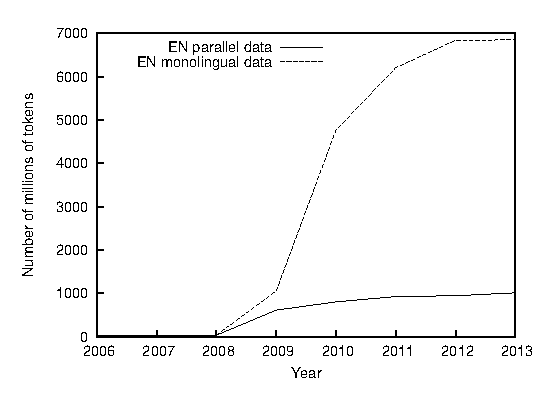
\includegraphics{figures/wmt/wmtdata.eps}
    \caption{Number of English tokens (in millions) in parallel and monolingual
      data available for the WMT French-English constrained track translation
      shared task for the years 2006 to 2013.}
    \label{fig:wmtdata}
  \end{center}
\end{figure}
%
Along with growing amounts of data, the use of more powerful computers
and distributed computing models such as
% rather than to paper
MapReduce~\citep{dean-ghemawat:2008:ACM,lin-dyer:2010:book} has enabled machine % TODOFINAL refer to background
translation researchers to build larger statistical machine translation models.
%Indeed, MapReduce was originally designed to process large datasets for parallelizable
%algorithms.
%
% notes on brants et al 2007 paper
% uses cutoffs
% p(w_i | w_{i - k + 1}^{i - 1}) = rho(w_{i - k + 1}^i) if w_{i - k + 1}^i is found
% = lambda(w_{i - k + 1}^{i - 1}) p(w_{i - k + 2}^i) o/w
% sb not a probability not a problem: it's just a feature scaled appropriately by mert
% vocabulary generation
% word to integer id conversion
% cutoff: words occurring less than threshold mapped to UNK
% vocabulary generation done with mapreduce
% mapreduce program is simply the canonical word count program
% generation of n-grams
% same as word count but with ngrams
% partition function that computes hash on first words of the n-gram
% use hash based on first 2 words
% needs to store unigram counts on all shards, as well as the corpus size N
% language model generation
% this is done online from what i understand
% given an n-gram, a particular shard is contacted
% there is further sharding from ngrams and their count
% but the last two words of the n-grams and also unigrams need to be stored again
% decoder architecture: store 1000-10000 ngrams then send them
% to the servers and compute sb probas on the fly
% search procedure
% current graph. then advance one word in source language,
% expand active hypotheses, queue up necessary ngrams,
% ask for scores, score expanded hypotheses and prune
%
MapReduce has thus been applied to various steps of the
translation
pipeline:
word alignment~\citep{dyer-cordova-mont-lin:2008:WMT},
translation model building~\citep{dyer-cordova-mont-lin:2008:WMT}
and
language
modelling~\citep{brants-popat-xu-och-dean:2007:EMNLP-CoNLL}.
We review these applications of MapReduce in more detail
in \autoref{sec:relatedwork}. The challenge is to find
effective modelling techniques that can be implemented
in the MapReduce framework.

However, once SMT models such as language models and translation
grammars are built, either with MapReduce
or some other method, the models must be made usable
by translation decoders, which only need a fraction of the information
contained in those models to be able to translate an input source sentence or a
set of input source sentences. For example, in translation from French to
English with a phrase-based
model (see \autoref{sec:phraseBasedTranslation}),
given an input sentence \emph{Salut toi}, we only need to know the
translation probabilities the translation model assigns to translations of
the words
\emph{Salut} and \emph{toi} and to translations of the phrase \emph{Salut toi}.
Similarly, given a test set, a decoder
only needs to retrieve the rules whose source side matches part of one of the source
sentences in the test set to be able to generate hypotheses.
With large models, simply retrieving relevant rules together with their
translation
probabilities becomes a challenge.

In the system
described by \citet{iglesias-degispert-banga-byrne:2009:NAACL},
given a training parallel corpus, rules are extracted and target
phrases and hierarchical phrases with counts are stored on disk.
Then, given an input test set, rules are extracted from the parallel
corpus a second time. Only rules relevant to the test set
are retained: source sides of phrase-based rules have to match
an $n$-gram from the test set and consecutive terminals
in source sides of hierarchical rules also have to match
an $n$-gram from the test set. As a consequence, some hierarchical
rules are never used in decoding. % TODOFINAL give an example
Source sides and rules together with their counts are kept
in memory using hash map datastructures, target sides with counts
are loaded from disk as precomputed in the first step, so that
source-to-target and target-to-source probabilities can be computed.

This
method becomes progressively slower with larger amounts of data
because it requires extracting rules from the training parallel corpus
and recomputing translation probabilities
each time we translate a new test set or a new
sentence. We
would like to improve on this design for more rapid experimentation. We also would like
to use a computing infrastructure that requires minimal maintenance. For example,
HBase\footnote{\url{http://hbase.apache.org}}, the open source non-relational database
implementation of
BigTable~\citep{chang-dean-ghemawat-hsieh-wallach-burrows-chandra-fikes-gruber:2008:ACM}, has been applied to the use of distributed language
models~\citep{yu:2008:mastersthesis}. However, we wish to address the question
whether we can adapt this infrastructure to our purposes with minimal
effort and without having to resort to database maintenance.
Rule filtering, i.e. the retrieval of rules relevant to the translation
of a test set or a sentence, is an essential step in our pipeline that can be a
bottleneck. Our goal is to reduce its processing time from several hours to a
few minutes.

In this chapter, we address the problem of retrieving relevant rules with their
translation probabilities. We report on investigations into
storing the model in the HFile data
structure. To our knowledge, this is the first
detailed proposed implementation of translation model storage and
filtering using HFile data structures. We find that this approach
offers a good compromise
between speed, performance and ease of implementation. The infrastructure necessary
for filtering is lightweight and requires the use of only one machine. We will
apply this approach to test set rule filtering prior
to decoding. We will discuss alternative
strategies as well as their strengths and weaknesses in terms of speed and
memory usage. In \autoref{sec:relatedwork}, we will review approaches that
have been used for model building and model filtering.
The HFile data structure that is used to
store models will be presented in \autoref{sec:hfile}.
In \autoref{sec:rulextractMapReduce}, we detail our custom implementation
of rule extraction and translation model estimation using
MapReduce. Our method and
alternative strategies for rule filtering are compared empirically in
\autoref{sec:rulextract}. We conclude in \autoref{sec:conclusion}.

\section{Related Work}
\label{sec:relatedwork}

In this section, we review applications of MapReduce to
the translation pipeline as well as techniques for storing
and retrieving from SMT models.

\subsection{Applications of MapReduce to SMT}
\label{sec:applicationsMapReduceSMT}

\citet{brants-popat-xu-och-dean:2007:EMNLP-CoNLL}
introduce a new smoothing method called
\emph{Stupid Backoff} (see \autoref{sec:stupidBackoffSmoothing}).
The Stupid Backoff smoothing scheme is recalled in \autoref{eq:stupidBackoffSchemeReminder}:
%
\begin{equation}
  p_{\text{stupid backoff}}(w_i \mid w_{i - n + 1}^{i - 1}) =
  \begin{cases}
    \frac{c(w_{i - n + 1}^i)}{c(w_{i - n + 1}^{i - 1})} & \text{if } c(w_{i - n + 1}^i) > 0 \\
    \alpha \, p_{\text{stupid backoff}}(w_i \mid w_{i - n + 2}^{i - 1}) & \text{if } c(w_{i - n + 1}^i) = 0
  \end{cases}
  \label{eq:stupidBackoffSchemeReminder}
\end{equation}
%
With respect to the traditional backoff scheme, the Stupid Backoff
scheme uses no discounting and simply uses relative frequency
for the non backed-off score and the backed-off score
scaling parameter is independent of
the $n$-gram history.
Therefore this scheme does not define a conditional probability
distribution % TODOFINAL add the word conditional in background
over a word given its history.

The Stupid Backoff language model building and application fit the
MapReduce framework well. The input to language model building
is a large monolingual corpus. The first step is to build
a vocabulary. This is done with the canonical example of word
counting with MapReduce. Counts % (see TODOFINAL refer to background)
are needed in order to remove words occurring less than a threshold
from the vocabulary. The second step is to obtain $n$-grams and their
count. This is done again with MapReduce, and the \emph{map} and \emph{reduce}
functions are analogous to the ones defined for word counting but this time
unigrams are replaced by $n$-grams.
For $n$-gram counting, the partition, or sharding, function hashes
on the first two words of each $n$-gram. In addition, unigram counts
and the total size of the corpus is available in each partition, i.e.
to each reducer. This allows relative frequencies to be computed.
\citet{brants-popat-xu-och-dean:2007:EMNLP-CoNLL} also
demonstrate
that for large amounts of monolingual data, i.e. above 10 billion
tokens, Stupid Backoff smoothing and Kneser-Ney smoothing perform comparably.
In addition, only
Stupid Backoff smoothing can be scaled to datasets
with more than 31 billion tokens. The scalability of Kneser-Ney
smoothing has been improved in recent work~\citep{heafield-pouzyrevsky-clark-koehn:2013:ACL}.\footnote{see also \url{http://kheafield.com/code/kenlm/estimation/}, Scalability section}

\citet{dyer-cordova-mont-lin:2008:WMT}
observe that translation model estimation has become prohibitive
on a single core and that existing \emph{ad hoc} parallelisation
algorithms may be more fragile than using an existing framework such
as the Hadoop implementation of
MapReduce.\footnote{\url{https://hadoop.apache.org/}}
They provide solutions to word alignment model
estimation and translation rule extraction and estimation using MapReduce
and demonstrate the scalability of their method.

The convenience
of the MapReduce framework for parallelisation has led to the building
of end-to-end toolkits for entire phrase-based~\citep{gao-vogel:2010:PBML} and
hierarchical phrase-based models~\citep{venugopal-zollmann:2009:PBML}
for translation using the MapReduce framework.

\subsection{SMT Models Storage and Retrieval Solutions}

We now review techniques appearing in the literature that have been used to
store SMT models and to retrieve the information needed in translation from
these models. SMT models are usually discrete probabilistic models and can
therefore be represented as a set of key-value pairs. To obtain relevant
information from a model stored in a certain data structure, a set of keys called a
\emph{query set} is formed; each key in this query set is then sought in that
datastructure. Strategies include:
%
\begin{itemize}
  \item storing the model as a simple data structure in memory
  \item storing the model in a text file
  \item storing the model in more complicated data structures such as
    tries~\citep{fredkin:1960:ACM} (in memory or disk)
  \item storing fractions of the entire model
  \item storing data as opposed to a precomputed model
  \item storing models in a distributed fashion
\end{itemize}
%
Each of these
strategies is discussed below.

In some cases, it may be possible to fit a model into RAM. In
this case the model can be stored as a memory associative array, such as a hash
table. In-memory storage allows allows for faster query retrieval than
on-disk storage, however only smaller models will fit in memory.
In-memory storage has been used to store model
parameters between iterations of expectation-maximisation for word
alignment~\citep{dyer-cordova-mont-lin:2008:WMT,lin-dyer:2010:book}.
% TODOFINAL somehow cite work by matei zaharia

For larger models, the set of key-value pairs can be stored as a table in a
single text file on local disk. Values for keys in the query set can be retrieved
by scanning through the entire file. For each key in the file, its membership is
tested in the query set. This is the approach adopted in the \emph{Joshua 5.0}
decoder~\citep{post-ganitkevitch-orland-weese-cao-callisonburch:2013:WMT}\footnote{Inferred from the decoder training
scripts available at \url{http://joshua-decoder.org/5.0/index.html}.}, which
uses regular expressions or $n$-grams to test
membership (see \autoref{sec:joshuaFiltering}).
\citet{venugopal-zollmann:2009:PBML} use MapReduce to scan a file concurrently:
the \emph{map} function tests if the vocabulary of a rule matches the
vocabulary of a test set.

The model can also be stored using a trie associative
array~\citep{fredkin:1960:ACM}. A trie is a type of tree where each node
represents a shared prefix of a set of keys represented by the child nodes. Each
node only stores the prefix it represents. The keys are therefore compactly
encoded in the structure of the trie itself. Querying the trie is a
$\mathcal{O}(\log(n))$ operation, where $n$ is the number of keys in the
dataset. The trie may also be small enough to fit in physical memory to further
reduce querying time. \citet{zens-ney:2007:HLTNAACL} use tries
to store a phrase-based grammar. All the source phrases are represented
in a trie stored on disk. Only relevant parts of the trie are loaded into
memory when a source phrase is sought.
\citet{ganitkevitch-cao-weese-post-callisonburch:2012:WMT} extend this
approach to store hierarchical phrase-based grammars. Both
source sides and target sides are stored in a packed representation of a trie.
Packed tries have also been applied for storing language
models~\citep{pauls-klein:2011:HLTACL,heafield:2011:WMT}.

It is also possible to create a much smaller approximate version of the model.
\citet{talbot-osborne:2007:ACL} represent a set of $n$-grams as a Bloom
filter~\citep{bloom:1970:ACM}.
They first use a standard Bloom filter to define a binary feature that
indicates whether an $n$-gram was seen in a monolingual corpus. They
also use a Bloom filter to encode $n$-grams together with quantised counts
in order to define a multinomial feature, that is a feature
with a finite set of possible values---in this case the quantised values. Both these data structure can
substantially reduce the disk space and memory usage with respect to lossless
representations of language models. However, they allow
false positives for $n$-gram
membership queries and overestimates of $n$-gram quantised counts. The authors
demonstrate that the features they introduce are useful in translation, despite
this lack of exactness.
In a related publication~\citep{talbot-osborne:2007:EMNLP-CoNLL}, the authors
demonstrate how these techniques can be used as a replacement to represent
a smoothed language model. \citet{talbot-brants:2008:ACL} use a Bloomier
filter~\citep{chazelle-kilian-rubinfeld-tal:2004:ACM-SIAM}
to represent $n$-grams and necessary statistics such as probabilities and backoff
weights. Unlike Bloom filters that only support Boolean characteristic
functions on a set, Bloomier filters support arbitrary functions, in this case
a mapping between an $n$-gram and its statistics. False positives can still occur
but for true positives, correct statistics are retrieved.

% TODOFINAL explain this better
%talbot-brants acl
%represent ngrams, proba, backoff with hash
%randomized language model
%kind of error: false positive but when ngram found, params are correct
%based on bloomier filter
%bloomier filter allows for arbitrary function as opposed to binary function

\citet{guthrie-hepple:2010:EMNLP} propose an extension to previous work
on randomised language models~\citep{talbot-osborne:2007:EMNLP-CoNLL} which prevents
the random corruption of model parameters but does not stop the random
assignment of parameters to unseen $n$-grams.
\citet{levenberg-osborne:2009:EMNLP} extend randomised language models to
stream-based language models. Another way of building a smaller approximate
version of a model is to retain items with high frequency counts from a stream
of data~\citep{manku-motwani:2002:VLDB}. This technique has been applied to
language modelling~\citep{goyal-daumeiii-venkatasubramanian:2009:NAACL} and
translation rule extraction~\citep{przywara-bojar:2011:PBML}. 


%talbot acl
%use bloom filter
%use standard bloom filter to test whether ngram was seen
%use log-frequency bloom filter to add frequency information
%ngram counts are quantised
%log frequency bloom filter: (ngram,1) (ngram,2) ... (ngram, quantizedcount(ngram)) inserted into the BF
%at retrieval time, we get back a count equal or greater than the actual quantized count
%trick to reduce error: c(w1-wn) < min(c(w1-wn-1), c(w2,wn))
%bloom filter language model test: use binary feature
%log-frequency bf lm: use the quantized count
%experiments: those features are useful in translation

%talbot emnlp
%this time not just binary features, but the whole lm estimated
%still use a log-frequency bf
%new: expected value of count
%E[c(x)|qc(x)=j] = (b^{j-1} + b^j - 1) / 2
%ccl: replacement for usual lm, use less space and memory

Instead of doing some precomputation on a dataset, it is possible to compute
the sufficient
statistics at query time using a suffix array~\citep{manber-myers:1990:SIAM}, so
that the model can be estimated only when needed. A suffix array is a sequence of
pointers to each suffix in a training corpus. The sequence is sorted with
respect to the lexicographic order of the referenced suffixes. Suffix arrays
have been used for computing statistics for language
models~\citep{zhang-vogel:2006:techreport}, phrase-based
systems~\citep{callisonburch-bannard-schroeder:2005:ACL,zhang-vogel:2005:EAMT},
and hierarchical phrase-based systems~\citep{lopez:2007:EMNLP-CoNLL}.
\citet{callisonburch-bannard-schroeder:2005:ACL} store both the source side
and the target side of a parallel corpus in two suffix arrays. They also maintain
an index between a position in the source or target side of the corpus and the
sentence number. During decoding, all occurrences of a source phrase
are located in the suffix array representing the source side of the corpus.
This produces a source marginal count. For each of these occurrences, the corresponding
sentence pair and word alignment are retrieved and rules are extracted. This produces
a rule count, which is normalised with the source marginal count to produce a
source-to-target probability. \citet{lopez:2007:EMNLP-CoNLL} extends this approach
to address the grammar extraction and estimation of hierarchical rules.
Note that the use of suffix arrays for translation model estimation only
supports the computation of source-to-target probabilities.

% TODOFINAL explain suffix array better
%suffixarray callisonburch
%suffix array for source corpus
%suffix array for target corpus
%index between sentence number and position in corpus (src and target)
%word alignment

%compute s2t probability
%locate all occurrences of f: gives c(f)
%for each occurrence of f, retrieve sentence pair and alignment
%run extraction: gives c(f, e)
%compute c(f, e) / c(f)

Finally, some approaches store language models in a distributed fashion.
We saw in \autoref{sec:applicationsMapReduceSMT} how a Stupid Backoff language
model can be built. After relative frequencies have been computed, another
partition function that hashes on the last two words of an $n$-gram is applied
so that backoff operations can be done withing the same partition.
At decoding time, the decoder architecture is modified in order
to request a batch of $n$-grams rather than a single $n$-gram.
The Stupid Backoff language model building can be scaled
to a corpus of 2 trillion tokens and the language model distributed
application can be made real time.

\citet{zhang-hildebrand-vogel:2006:EMNLP} propose a distributed large language
model backed by suffix arrays. HBase has also been used to build a distributed
language infrastructure~\citep{yu:2008:mastersthesis}. The method we propose to
use is closely related to the latter but we use a more lightweight
infrastructure than HBase. In addition, it is also possible to apply our method
to language model querying~\citep{pino-waite-byrne:2012:PBML}, which
demonstrates the flexibility of the infrastructure.

\section{HFile Description}
\label{sec:hfile}

We now describe the data structure we use to store models and we review relevant
features to the design of our system. To store a model represented as key-value
pairs, we use the HFile file format,\footnote{\url{http://hbase.apache.org}} which is
a open source reimplementation of the SSTable file
format~\citep{chang-dean-ghemawat-hsieh-wallach-burrows-chandra-fikes-gruber:2008:ACM}.
The HFile format is a lookup table with key and value columns. The entries are free
to be an arbitrary string of bytes of any length. The table is sorted
lexicographically by the key byte string for efficient record retrieval by key.

\subsection{HFile Internal Structure}

% TODOFINAL read SSTable description
% TODOFINAL check whether blocks are plural or singular

\paragraph{High Level Structure} As can be seen in \autoref{fig:hfile},
the HFile internal structure is divided into blocks. There are various types of
block, depending on the kind of information a block contains.
In order to
distinguish block types, the first 8 bytes of a
block will indicate its type. The blocks are grouped into
three parts. The first part (top) is organised into
data blocks interleaved with leaf data index blocks and Bloom blocks.
The second part (middle) consists of intermediate data index blocks.
The third part (bottom) consists of metadata: root data index blocks, a file
information block and a Bloom filter index block.

\paragraph{Index Blocks} The root data index blocks map keys to their
relevant intermediate data index block, indicated by
an offset. In turn, an intermediate data index block
maps keys to their relevant leaf data index block, again indicated by an offset.
Finally, a leaf data index block maps keys to their relevant data block,
still indicated by an offset. The same mechanism is employed for the Bloom filter.
The Bloom filter index block maps keys to their relevant Bloom block.

\paragraph{Block Size Configuration} The block size is
configurable, with a default size of 64KB. Note that HFile blocks are not to be
confused with Hadoop Distributed File System (HDFS) blocks whose default size is
64MB.

\paragraph{Block Compression} The HFile format allows for
the blocks to be compressed. The choice of compression codec is selected when
the file is created. We choose the GZip compression
codec~\citep{Deutsch:1996:ZCD:RFC1950} for all our % TODOFINAL check that the gzip cite is correct
experiments.
%Block compression is also used in other related
%software~\citep{pauls-klein:2011:HLTACL}. % TODOFINAL reread paper and elaborate

\begin{figure}
  \begin{center}
    \begin{tabular}{|l|}
      \hline
      \rowcolor[gray]{0.85}
      Data Block \\
      \hline
      \rowcolor[gray]{0.85}
      ... \\
      \hline
      \rowcolor[gray]{0.95}
      Leaf Data Index Block / Bloom Block \\
      \hline
      \rowcolor[gray]{0.85}
      ... \\
      \hline
      \rowcolor[gray]{0.85}
      Data Block \\
      \hline
      \rowcolor[gray]{0.85}
      ... \\
      \hline
      \rowcolor[gray]{0.95}
      Leaf Data Index Block / Bloom Block \\
      \hline
      \rowcolor[gray]{0.85}
      ... \\
      \hline
      \rowcolor[gray]{0.85}
      Data Block \\
      \hline
      \hline
      \rowcolor[gray]{0.9}
      Intermediate Data Index Blocks \\
      \hline
      \hline
      \rowcolor[gray]{0.7}
      Root Data Index Blocks \\
      \hline
      \rowcolor[gray]{0.7}
      File Info Block \\
      \hline
      \rowcolor[gray]{0.7}
      Bloom Filter Index Block \\
      \hline
    \end{tabular}
    \caption[Caption for LOF]{HFile internal structure.\footnotemark \ The
      structure is divided into three parts. In the first part, data blocks
      are interspersed with leaf data index blocks and Bloom blocks. The second
      part contains intermediate data index blocks. The third part consists
      of metadata: root data index blocks, file format information and a Bloom
      filter index block.}
    \label{fig:hfile}
  \end{center}
\end{figure}

\footnotetext{After \url{http://hbase.apache.org/book/book.html} (simplified)}

\subsection{Record Retrieval}
\label{sec:recordRetrieval}

When the HFile is opened for reading, the root data index blocks are loaded into memory.
To retrieve a value from the HFile given a key, the appropriate intermediate
index block is located by a binary search through the root data index. Binary
searches are conducted on the intermediate and leaf index blocks to identify the
data block that contains the key. The identified data block is then loaded off the disk
into memory and the key-value record is retrieved by scanning the data block
sequentially.

\subsection{Bloom Filter Optimisation for Query Retrieval}
\label{sec:bloomFilterOptimization}

It is possible to query for a key that is not contained in the HFile. This very
frequently happens in translation because of language data sparsity: in our case,
because keys are $n$-grams of terminals and nonterminals, the number of possible
keys is exponential in the size of the vocabulary, and many of these
will not have been observed in any rule extracted from training data.

Querying
the existence of a key is expensive as it involves all the operations
described in \autoref{sec:recordRetrieval}: loading and binary
searching the root data index,
loading and binary searching an intermediate data index block,
loading and binary searching
a leaf data index block and finally loading and scanning a data block.

For fast existence check queries, the HFile format allows
the inclusion of an optional Bloom filter~\citep{bloom:1970:ACM}. A Bloom filter
provides a probabilistic, memory efficient representation of the key set with a
$\mathcal{O}(1)$ membership test operation. The Bloom filter may provide a false
positive, % TODOFINAL expand on Bloom filters somewhere either background or here
but never a false negative, for existence of a key in the HFile.
Therefore, it is safe to use in our setting as some keys will be looked
up in the HFile even though they are not present, but the situation
where keys that are in the HFile are not looked up will not happen.

For a large
HFile, the Bloom filter may also be very large. Therefore the  Bloom filter is
also organised into blocks called Bloom blocks. Each block contains a smaller
Bloom filter that covers a range of keys in the HFile. Similar to the root data
index, a Bloom index is constructed. To check for the
existence of a key, a binary search is conducted on the Bloom index, the
relevant Bloom block is loaded, and the membership test performed.

Unlike work on Bloom filter language
model~\citep{talbot-osborne:2007:ACL,talbot-osborne:2007:EMNLP-CoNLL}, this
filter only tests the existence of a key and does not return any statistics from
the value. If a membership test is positive, a usual key search will
still be carried out. During the execution of a query, two keys may
reference the same index or Bloom blocks. To prevent these blocks from being
repeatedly loaded from disk, the blocks are cached after reading.

\subsection{Local Disk Optimisation}

The HFile format is designed to be used with HDFS, a distributed file system
based on the Google File System~\citep{ghemawat-gobioff-leung:2003:OSP}. Large
files are split into HDFS blocks that are stored on many nodes in a cluster.
However, the HFile format can also be used completely independently of HDFS. If
its size is smaller than local disk space, the entire HFile can be stored on the local
disk of one machine and accessed through the machine's local file system. We
report in \autoref{sec:rulextract} that using local disk
is faster than using HDFS.

\subsection{Query sorting optimisation}
\label{sec:querySortingOptimization}

Prior to HFile lookup, we sort keys in the query set lexicographically. If two
keys in the set of queries are contained in the same block, then the block is
only loaded once. In addition, the computer hardware and operating system allow
further automatic improvements to the query execution. Examples of these
automatic improvements include reduced disk seek time,
caching data from
disk by the operating system,\footnote{The Linux Documentation Project, The File System, \url{http://tldp.org}}
or CPU caching data from main memory~\citep{patterson-hennessy:2005:COA}.

\section{Hierarchical Rule Extraction with MapReduce}
\label{sec:rulextractMapReduce}

In the previous section, we have described the HFile format. We will use
this format to store a translation grammar. In this
section, we describe how we generate this grammar and produce the HFile
that represents the grammar.
We describe a MapReduce implementation of hierarchical grammar
extraction and estimation. The implementation is an
extension of \emph{Method 3} described by
\citet{dyer-cordova-mont-lin:2008:WMT}, which was originally developed
to estimate translation probabilities for phrase-based models.

MapReduce~\citep{dean-ghemawat:2008:ACM} is a framework designed for processing
large amounts of data in a distributed fashion on a computer cluster. In this
framework, the programmer needs to implement a function called \emph{map} and
a function called \emph{reduce}. The \emph{map} function is defined in
\autoref{eq:mapFunction}:
%
\begin{equation}
  \text{map} : (k_1, v_1) \longmapsto [(k_2, v_2)]
  \label{eq:mapFunction}
\end{equation}
%
where $(k_1, v_1)$ is a key-value pair and $[(k_2, v_2)]$ is a list of
key-value pairs. We use the $[ \, ]$ notation to denote a list. Keys and values are arbitrary byte sequences. As the key-value
pairs $(k_2, v_2)$ are computed by the \emph{map function}, the MapReduce framework groups all values $v_2$ by key $k_2$ in order
to provide an input $(k_2, [v_2])$ to the \emph{reduce} function, defined in
\autoref{eq:reduceFunction}:
%
\begin{equation}
  \text{reduce} : (k_2, [v_2]) \longmapsto [(k_3, v_3)]
  \label{eq:reduceFunction}
\end{equation}
%
The input to the \emph{reduce} function is a key and a list of values. The
\emph{reduce} function generates a list of key-value pairs.

Using this notation, % TODOFINAL refere to background
we can describe the grammar extraction and estimation
as a series of MapReduce jobs, summarised in
\autoref{fig:ruleXtractionPipeline}.
%
\begin{figure}
  \tikzstyle{MapReduceJob} = [rectangle, draw, fill=blue!20, rounded corners,
    align = left, text width = 3.5cm]
  \tikzstyle{JobInputOutput} = [draw, ellipse,fill=red!20,
    align = left, text width = 2.9cm]
  \tikzstyle{line} = [draw, very thick, color=black!50, -latex']

%\begin{center}
\begin{tikzpicture}[node distance = 2.2cm]
  \begin{normalsize}
    % Place nodes
    \node [JobInputOutput, text width = 6cm] (corpus) {
      $k_1$ : metadata \\
      $k_2$ : word-aligned sentence pair
    };
    \node [MapReduceJob, below of=corpus, text width = 7cm] (extract) {
      \textbf{Rule Extraction} (see \autoref{sec:hierruleextract}) \\
      \emph{map} : extract rules \\
      \emph{reduce} : none};
    \node [JobInputOutput, below of=extract] (rules) {
      $k_1$ : rule \\
      $k_2$ : metadata};
    \node [MapReduceJob, below left = 1cm and -1.5cm of rules, text width = 6.5cm] (s2t) {
      \textbf{Source-to-target Probability} \\
      \emph{map} : output (\emph{src}, (\emph{trg}, 1)) \\
      \emph{reduce} : sum \emph{trg} counts, normalise};
    \node [MapReduceJob, below right = 1cm and -1.5cm of rules, text width = 6.5cm] (t2s) {
      \textbf{Target-to-source Probability} \\
      \emph{map} : output (\emph{trg}, (\emph{src}, 1)) \\
      \emph{reduce} : sum \emph{src} counts, normalise};
%    \node [MapReduceJob, below = 1.2cm of rules] (other) {\textbf{Other MapReduce Feature}};
    \node [JobInputOutput, below = 0.7cm of s2t, text width = 4.4cm] (rulesPlusS2t) {
      $k_1$ : rule \\
      $k_2$ : source-to-target pr};
    \node [JobInputOutput, below = 0.7cm of t2s, text width = 4.4cm] (rulesPlusT2s) {
      $k_1$ : rule \\
      $k_2$ : target-to-source pr};
%    \node [JobInputOutput, below = 1.7cm of other] (rulesPlusOther) {$k_1$: rule \\
%                                                                   $k_2$: other feature};
    \node [MapReduceJob, below = 5.7cm of rules, text width = 8.5cm] (merge) {
      \textbf{Merge} \\
      \emph{map} : output (\emph{src}, (\emph{trg}, feature)) \\
      \emph{reduce} : output (\emph{src}, list of \emph{trg} and features)};
    \node [JobInputOutput, below = 1cm of merge, text width = 5cm] (ruleAllFeatures) {
      $k_1$ : \emph{src} \\
      $k_2$ : list of \emph{trg} and features};
    % Draw edges
    \path [line] (corpus) -- (extract);
    \path [line] (extract) -- (rules);
    \path [line] (rules) -- (s2t);
    \path [line] (rules) -- (t2s);
%    \path [line] (rules) -- (other);
    \path [line] (s2t) -- (rulesPlusS2t);
    \path [line] (t2s) -- (rulesPlusT2s);
%    \path [line] (other) -- (rulesPlusOther);
%    \path [line] (rulesPlusOther) -- (merge);
    \path [line] (rulesPlusS2t) -- (merge);
    \path [line] (rulesPlusT2s) -- (merge);
    \path [line] (merge) -- (ruleAllFeatures);
    \end{normalsize}
\end{tikzpicture}
%\end{center}
\caption{Translation grammar extraction and estimation pipeline as a series of MapReduce jobs. Ellipses
represent (intermediate) input/output of MapReduce jobs. Rectangles represent
MapReduce jobs. Source, target and probability are abbreviated into
src, trg and pr. Rules are first extracted, then the source-to-target and
target-to-source translation models are estimated. Finally, the features,
i.e. the translation models, are merged and the final output has rules sources
as keys and lists of targets with features as values.}
\label{fig:ruleXtractionPipeline}
\end{figure}

\subsection{Rule Extraction}

The first step in grammar extraction and estimation is rule extraction. For
this step, $v_1$ represents a sentence pair together with a word alignment and $k_1$
contains metadata about the parallel corpus such as what collection the sentence
pair comes from. This kind of information is useful for domain adaptation as
demonstrated in \autoref{sec:domainAdaptationGrammar}. The \emph{map}
function simply extracts hierarchical rules for
that sentence pair and outputs the rules. $k_2$ is a rule and $v_2$ contains
the metadata from $k_1$. For rule extraction, there is no reduce step.
\autoref{eq:mapIllustrationRuleXtraction} illustrates the \emph{map} function
for rule extraction:
%
\begin{equation}
  map : (\text{newswire}, (\bm{f}, \bm{e}, \bm{a})) \longmapsto [(r_1, \text{newswire}), (r_2, \text{newswire}),...]
  \label{eq:mapIllustrationRuleXtraction}
\end{equation}

\subsection{Corpus-Level Feature Computation}
Rule extraction is followed by several MapReduce jobs that are run simultaneously
in order to
compute \emph{corpus-level} features. Corpus-level features
are features related
to each rule and the computation of which requires looking at the entire set of
extracted rules. In this description, we only consider source-to-target and
target-to-source probabilities, but many other corpus-level features are possible,
for example features that relate to the word alignment from which rules were
extracted. We use the metadata stored in the output of the
extraction job in order to compute collection specific probabilities.
Collection specific probabilities are probabilities computed over a specific subset
of the training corpus. The metadata indicates whether a rule was extracted from
that specific subset.

Let us
consider first the collection-specific source-to-target probability computation.
The input to the \emph{map} function
is the output of the extraction job, that is a rule together with metadata.
The \emph{map} function checks that the rule comes from the collection we are
interested in and if so, outputs the source of the rule as a key $k_2$ and the
target of the rule together with a count of one as a value $v_2$. Targets (and
counts) corresponding to the same source are grouped together by the MapReduce
framework. The input to the \emph{reduce} function is a source ($k_2$) and
a list of targets with counts ($[v_2]$). The \emph{reduce} function aggregates
the counts for the distinct targets and then normalises those counts with the
total count corresponding to the source $k_2$. The output of the \emph{reduce}
function is a list of pairs (rule, probability).

The target-to-source probability computation is very similar. Apart from
inverting the role played by source and target, the \emph{map} and \emph{reduce}
function also need to change the rule format for
rules that invert the order of nonterminals in the source
and the target, for example \RT[$X$][$X_1 a X_2$][$X_2 b X_1$].
%\emph{hierarchical reordering rules}. % TODOFINAL mention this in background
%A hierarchical reordering rule is a rule with two nonterminals that inverts the
%order of the nonterminals in the source and in the target. For example,
%\RT[$X$][$X_1 a X_2$][$X_2 b X_1$] is a hierarchical reordering rule.
For this
type of rule, the \emph{map} function has to invert the order of nonterminals
in both the source and target so that probabilities are computed correctly. For
example, the \emph{map} function will output the target of the rule
written as $X_1 b X_2$ and the source of the rule
written as $X_2 a X_1$. The \emph{reduce} function
will restore the original notation.

We have described the computation of
collection specific translation probabilities.
The source-to-target and target-to-source probabilities over the
entire corpus are computed in an identical manner with the
collection simply being the entire corpus.
\autoref{fig:ruleXtractionPipeline} illustrates only two corpus-level
features, however, in practice, more features are computed: source-to-target
and target-to-source probability for each collection and for the entire parallel
text, as well as lexical features (see \autoref{sec:features}).

\subsection{Feature Merging}

Once all MapReduce features have been computed, a MapReduce job that merges
the features is called. The input key $k_1$ to the \emph{map} function is a
rule and the input value $v_1$ is a feature. The \emph{map} function outputs
the source of the rule as a key $k_2$ and the target of the rule together with
the feature as value $v_2$. Targets and features corresponding to the same
source are grouped together by the MapReduce framework. The input to the
\emph{reduce} function is a source ($k_2$) and a list of targets with features
($[v_2]$). The \emph{reduce} function simply merges the features for identical
targets. The output key $k_3$ is the source $k_2$ and the output value $v_3$ is
a list of targets with all computed features.

The output of this merging job
is converted to an HFile format. Because the keys in the HFile format need to
be sorted, we also want the output of the merging job to be sorted by key. One
way to achieve this is to specify only one reducer for the job but this solution
is very slow because only one core will be used for the reduce step. A better
way is to use a \emph{TotalOrderPartitioner}. We first use a small amount of
data so that it may be feasible to carry out rule extraction with only one
reducer in the merge step. We use the output of this small scale extraction as
input to an \emph{InputSampler}. The sampler will generate a partition file for
the partitioner. The use of a \emph{TotalOrderPartitioner} will guarantee that
all keys are sorted after the reduce step. % TODOFINAL clear as mud, expand

\section{Hierarchical Rule Filtering for Translation}
\label{sec:rulextract}

In the previous section, we have described how to obtain an HFile
that represents a hierarchical translation grammar.
We will now describe how this datastructure can be used to retrieve rules for
a given test set efficiently. We describe our system called
\emph{ruleXtract}, and compare it to other methods through time and memory
measurements.

\subsection{Task Description}

Given a test set, defined as a set of sentences to be translated, and a
hierarchical phrase-based translation grammar, we would
like to retrieve all the relevant rules from the model. A phrase-based rule
in the HFile is
relevant if its source is a subsequence of a sentence in the test set. A
hierarchical rule in the HFile is relevant if
its source, where nonterminals are instantiated into
terminals, is
a subsequence of a sentence in the test set. For example, with a test set
containing one sentence \emph{Salut toi}, the phrase-based rules with sources
\emph{Salut}, \emph{toi}, \emph{Salut toi} are relevant and the hierarchical
rules with sources \emph{Salut X} and \emph{X toi} are relevant, because
instantiating \emph{Salut X} into \emph{Salut toi} produces a subsequence
of the test sentence and similarly for \emph{X toi}.

\subsection{HFile for Hierarchical Phrase-Based Grammars}
\label{sec:hfileForHiero}

% TODOFINAL explain better the source pattern instantiation business with an example.

% TODOFINAL maybe refer to background for pattern definition

Given a test set and an HFile storing a hierarchical phrase-based grammar, we
first generate queries from the test set, then retrieve relevant rules along
with their corpus-level features from the HFile. To generate queries, we have a set
of allowed \emph{source patterns} and instantiate these patterns against the
test set. Rule patterns were defined in \autoref{sec:hiergrammar}.
A source pattern is simply the source side of a rule pattern.
Here, we briefly redefine source patterns.
A source pattern is a regular expression that matches
the source side of a rule. For example, the
pattern $\Sigma^+X$, with $\Sigma$ the source vocabulary,
represents a rule source side containing a sequence of
terminals followed by the nonterminal X. If the input sentence is
\emph{Salut à toi}, the pattern will be instantiated as \emph{Salut X},
\emph{Salut à X} and \emph{à X}. We impose the following constraints on source pattern
instantiation where the first four relate to constraints in extraction and the
last one relates to a decoding constraint:
%
\begin{itemize}
  \item $s_{\text{max}}$: maximum number of terminals for phrase-based rules.
  \item $s_{\text{max elements}}$: maximum number of terminals and nonterminals.
  \item $s_{\text{max terminals}}$: maximum number of consecutive terminals for
    hierarchical rules.
  \item $s_{\text{max NT}}$: maximum nonterminal span in a hierarchical
    rule.
  \item $s_{\text{max span}}$: maximum span for the rule. This constraint
    is not to be confused with the previous $s_{\text{max NT}}$ constraint.
    While $s_{\text{max NT}}$ represents the maximum span of a nonterminal
    on the right hand side of a rule, $s_{\text{max span}}$ represents the maximum span
    of an entire rule, or alternatively the maximum span of the nonterminal on the left
    hand side of the rule. Because the latter constraint is enforced by the decoder, we
    also enforce it in source pattern instantiation so that rules that will
    never be used by the decoder are not generated.
\end{itemize}
%
The source pattern instances are then sorted for more efficient HFile lookup
(see \autoref{sec:querySortingOptimization}). Each
query is then looked up in the HFile and if
present, an HFile record is retrieved.
% TODOFINAL include this somewhere
%We typically run this retrieval step on one machine only.
We now compare our approach to similar approaches whose aim is
to obtain rules which are relevant to a test set.

\subsection{Suffix Arrays for Hierarchical Phrase-Based Grammars}

One alternative strategy for building a set specific grammar is to use
suffix arrays introduced in \autoref{sec:relatedwork}. We use the \emph{cdec}
software~\citep{dyer-lopez-ganitkevitch-weese-ture-blunsom-setiawan-eidelman-resnik:2010:ACL}
implementation of suffix arrays for
hierarchical phrase-based rule extraction. The \emph{cdec} implementation is based on
earlier work~\citep{lopez:2007:EMNLP-CoNLL} which extends suffix array based
rule extraction from phrase-based system
to hierarchical phrase-based systems (see again \autoref{sec:relatedwork}).

Given a test set, a set of source pattern instances is generated similarly to
what is done for \emph{ruleXtract}. These source pattern instances are then
sought in a suffix array compiled from the source side of a parallel corpus.
Rules are extracted using the word alignment, and source-to-target
probabilities are then computed as described in \autoref{sec:relatedwork}.

\subsection{Text File Representation of Hierarchical Phrase-Based Grammars}
\label{sec:joshuaFiltering}

We now describe the \emph{Joshua}
decoder~\citep{weese-ganitkevitch-callisonburch-post-lopez:2011:WMT}
implementation for storing and retrieving from a translation
model.
The first implementation variant, which we call \emph{Joshua}, stores the
translation model in a text file. Given a test set, each word in the test set
vocabulary is mapped to the list of sentences in which it appears. Then, each
rule in the translation model is compiled to a regular expression, and each
sentence that contains at least a vocabulary word of the rule is matched against
this regular expression. If at least one match is successful, the rule is
retained.

A faster version is provided that matches consecutive terminals in the
source side of a rule to the set of $n$-grams extracted from the test set. We
call this version \emph{Joshua Fast}. A parallel version also exists that chunks
the grammar file and distributes each chunk processing as a separate process on
a cluster running Sun Grid Engine~\citep{gentzsch:2001:CCG}. We call this
version \emph{Joshua Parallel}. The parallel version using the faster matching
algorithm is called \emph{Joshua Fast Parallel}.

\subsection{Experimental Design}

In this section, we describe our experimental setup in terms of data and various
configurations for grammar extraction, grammar filtering and
time and memory measurements.
%
\paragraph{Parallel Text} We use a small parallel corpus of 750,950 word-aligned sentence
    pairs and a larger corpus of 9,221,421 word-aligned sentence pairs from the
    NIST'12 Chinese-English evaluation, in order to investigate how systems perform % TODOFINAL footnote or cite for nist
    with varying amounts of parallel text and whether those systems are robust
    when dealing with larger data sets.
%
\paragraph{Grammar Extraction} From the parallel corpora, we extract hierarchical
    grammars with the source-to-target probability feature only. This is done
    because we do
    not want feature computation to introduce variability in timing results when
    comparing different strategies and software implementations. In addition, not
    all systems can generate the same set of features. For example,
    the suffix array implementation of rule extraction is not able to generate
    target-to-source probabilities. Note that in practice for
    translation decoding, given a vector of
    parameters, we could simply replace multiple features in the translation
    model by a single value representing the dot product of the features with
    the parameter vector. However, we need to keep separate feature values for
    optimisation (see \autoref{sec:mert}).

    The rule extraction constraints described in \autoref{sec:hfileForHiero}
    are set as follows:
%
\begin{itemize}
  \item $ s_{\text{max}}= 9$
  \item $s_{\text{max elements}} = 5$
  \item $s_{\text{max terminals}} = 5$ % TODOFINAL explain why it's redundant or change value
  \item $s_{\text{max NT}} = 10$ % TODOFINAL (done ?) harmonize notation with extraction from posteriors and from background
\end{itemize}
%
With these settings, the small grammar contains approximately 60M rules while the 
larger grammar contains approximately 726M rules. The grammars we obtain are
converted to the \emph{Joshua} format in order to be able to filter them
with the \emph{Joshua} decoder. We do not generate a hierarchical grammar
with \emph{Joshua} simply because we want to compare the performance of
rule retrieval from the same grammar.
%
\paragraph{Grammar filtering} For \emph{ruleXtract}, we use the following constraints for
    source pattern instantiation: 
    \begin{itemize}
      \item $ s_{\text{max}} = 9$
      \item $s_{\text{max elements}} = 5$
      \item $s_{\text{max terminals}} = 5$ % TODOFINAL explain why redundant with max source elements
      \item $s_{\text{max NT}} = \infty$
      \item $s_{\text{max span}} = \infty$ % TODOFINAL (done ?) explain diff between hrmaxheight and max nt: max nt is the max span of an X on the rhs whereas hrmaxheight is the max span of the source of a rule, i.e. max span of X on the lhs
    \end{itemize}
    %
    These settings are chosen so that the number of rules obtained after filtering is identical between
    \emph{ruleXtract} and \emph{Joshua}. Thus, time and memory measurements
    are comparable. % TODOFINAL explain better.
%
\paragraph{Measurements} We report time measurements for query processing and query
    retrieval and the total time used to obtain a set specific rule file for a
    test set of 1755 Chinese sentences and 51008 tokens. We also report peak
    memory usage. For \emph{ruleXtract}, query processing involves generating
    source pattern instances and sorting them according to the HFile sorting order.
    If we use a Bloom filter, it also involves pre-filtering the queries with
    the Bloom filter. Query retrieval involves HFile lookup. For the
    \emph{Joshua} configurations, query processing involves indexing the test
    set and generating test set $n$-grams and query retrieval involves regular
    expression matching.

    For the \emph{Joshua Parallel}
    configurations, we use 110 jobs for the larger grammar on a cluster of 9
    machines. For this latter configuration, we report the maximum time spent on
    a job (not the sum) and the maximum memory usage by a job.
%
\paragraph{Hardware configuration} the machine used for query processing has 94GB of
    memory and an Intel Xeon X5650 CPU. The distributed file system is hosted on
    the querying machine and other machines with the same specification, which
    are used to generate the HFile.

Our experimental setup was designed for accurate comparisons between alternative
strategies for grammar filtering. In practice, an end-to-end translation
system need not use this exact setup. For example the grammar extracted by \emph{Joshua} is
in general smaller than the grammar extracted by \emph{ruleXtract} because \emph{Joshua}
includes target side constraints. On the other hand, \emph{ruleXtract} uses threshold
cutoffs, such as a minimum source-to-target translation probability, % TODOFINAL refer to background, TODOFINAL in background, actually talk about these cutoffs
in order to reduce the size of the test set specific grammar.

\subsection{Results and Discussion}

% TODOFINAL center the double rows rather than adding empty rows
\begin{table}[htbp]
  \footnotesize
  \begin{center}
  \begin{tabular}{*{7}{|l}|}
    \hline
    \multicolumn{7}{|c|}{{\bf Small Grammar}} \\
    \hline
    \textbf{Row} & {\bf System} & {\bf Query } & {\bf Query} & {\bf Total} & {\bf Peak } & {\bf \# Rules} \\
                & & {\bf Processing} & {\bf Retrieval} & {\bf Time} & {\bf Memory} & \\
    \hline
    1 & \emph{ruleXtract} & 9m1s & 7m36s & 16m40s & 40.8G & 6435124 \\
      & \emph{HDFS} & & & & & \\
    \hline
    2 & \emph{ruleXtract} & 8m57s & 2m16s & 11m15s & 39.9G & 6435124 \\
      & \emph{Bloom, HDFS} & & & & & \\
    \hline
    3 & \emph{ruleXtract} & 8m54s & 7m33s & 16m30s & 40.4G & 6435124 \\
      & \emph{Local} & & & & & \\
    \hline
    4 & \emph{ruleXtract} & 8m50s & 2m19s & 11m11s & 38.8G & 6435124 \\
      & \emph{Bloom, Local} & & & & & \\
    \hline
    5 & \emph{Joshua} & 0.9s & 29m51s & 29m54s & 42.2G & 6435124 \\
    \hline
    6 & \emph{Joshua} & 0.9s & 7m25s & 7m28s & 40.1G & 7493178 \\
      & \emph{Fast} & & & & & \\
    \hline
    \multicolumn{7}{|c|}{{\bf Large Grammar}} \\
    \hline
    \textbf{Row} & {\bf System} & {\bf Query } & {\bf Query} & {\bf Total} & {\bf Peak } & {\bf \# Rules} \\
                & & {\bf Processing} & {\bf Retrieval} & {\bf Time} & {\bf Memory} & \\
    \hline
    7 & \emph{ruleXtract} & 8m56s & 22m18s & 31m17s & 42.2G & 47978228 \\
      & \emph{HDFS} & & & & & \\
    \hline
    8 & \emph{ruleXtract} & 9m12 & 15m33s & 24m49s & 40.7G & 47978228  \\
      & \emph{Bloom, HDFS} & & & & & \\
    \hline
    9 & \emph{ruleXtract} & 8m55s & 21m3s & 30m1s & 41.6G & 47978228 \\
      & \emph{Local} & & & & & \\
    \hline
    10 & \emph{ruleXtract} & 9m0s & 14m43s & 23m46s & 40.6G & 47978228 \\
       & \emph{Bloom, Local} & & & & & \\
    \hline
    11 & \emph{Joshua} & 0.9s & out of & out of & out of & out of \\
       & &      & memory & memory & memory & memory \\
    \hline
    12 & \emph{Joshua} & 0.9s & out of & out of & out of & out of \\
       & \emph{Fast} &      & memory & memory & memory & memory \\
      & & & & & & \\
    \hline
    13 & \emph{Joshua} & 0.9s & 537m10s & 537m11s & 10.1G & 47978228 \\
       & \emph{No Cache} & & & & & \\
    \hline
    14 & \emph{Joshua} & 0.9s & 78m53s & 78m54s & 10.1G & 83339443 \\
       & \emph{Fast No Cache} & & & & & \\
    \hline
    15 & \emph{Joshua} & \multicolumn{3}{c|}{total time for slowest job: 43m36s} & 4G & 47978228 \\
       & \emph{Parallel} & \multicolumn{3}{c|}{} & & \\
    \hline
    16 & \emph{Joshua} & \multicolumn{3}{c|}{total time for slowest job: 44m29s} & 4G & 83339443 \\
       & \emph{Fast Parallel} & \multicolumn{3}{c|}{} & & \\
    \hline
  \end{tabular}
  \caption{Time and memory measurements for rule filtering with different
    strategies for a small and a large grammar. Various configurations for
    \emph{ruleXtract} and \emph{Joshua} are compared for time and memory
    usage. The \emph{fast} configuration for \emph{Joshua} filters rules
    by matching consecutive terminals to test set $n$-grams, which explains
    that the number of rules obtained is higher than in all other configurations.
    This also means that some filtered rules are never used in decoding.}
  \label{tab:ruleXtract}
  \end{center}
\end{table}

Results are summarised in \autoref{tab:ruleXtract}, from which we can draw the
following observations:
%
  % TODONEVER when pointing at rows, use hyperlinks
\paragraph{Speed} The \emph{Total Time} column shows that \emph{ruleXtract} is
    competitive with alternative strategies in terms of speed.
\paragraph{Memory} The \emph{Peak Memory} column shows that both \emph{ruleXtract} and
    \emph{Joshua} are memory hungry, with a usage of up to 40GB. In the case of \emph{ruleXtract},
    this is because we keep all source pattern instances for all test set
    sentences are kept in memory. In the case
    of \emph{Joshua}, this is due to a caching optimisation: rule source sides
    that have already been considered relevant to the test set are stored
    in a hash map.
\paragraph{Local disk optimisation} Comparing \emph{HDFS} and \emph{Local} rows
    (row 1 vs.\ row 3, row 2 vs.\ row 4, row 7 vs.\ row 9, row 8 vs.\ row 10), we can
    see that using the local filesystem as opposed to HDFS gives a small
    decrease in query retrieval time, which becomes more
    substantial for the larger grammar.
    This is because when the HFile is stored on HDFS, it is composed of several
    HDFS blocks that can be located on different data nodes.
    Since the HFile size is smaller than the disk space on each data node, it is preferable
    to store the HFile on local disk. However, because the HFile was generated on
    HDFS through a MapReduce job, this
    requires copying or moving the HFile from the HDFS file system to the
    local disk file system prior to running grammar retrieval.
\paragraph{Bloom filter optimisation} Comparing rows with and without \emph{Bloom}
    (row 1 vs.\ row 2, row 3 vs.\ row 4, row 7 vs.\ row 8 and row 9 vs.\ row 10), we can
    see that the
    use of a Bloom filter gives an important decrease in query retrieval time.
    This is due to the fact that the number of source pattern instances queries
    is 31,552,746 and after Bloom filtering, the number of queries is 1,146,554
    for the small grammar and 2,309,680 for the larger grammar, reducing the
    number of time consuming HFile lookups respectively by 96\% and 93\%. Note
    that Bloom filters increase query processing time only for the
    large grammar and more so when using HDFS.
\paragraph{Parallelisation} In order to run \emph{Joshua} on the larger grammar and
    avoid memory problems, we needed to use parallelisation, which provided
    competitive speeds and a low memory footprint (maximum 4G per job) (see rows
    15 and 16).

For comparison, \emph{cdec}'s total processing time is 57m40s for the small
grammar, which is significantly slower than the other methods. However, we do
not include \emph{cdec}'s suffix array implementation performance in
\autoref{tab:ruleXtract}
because the suffix array method involves much on-the-fly computation, such
as rule extraction and source-to-target probability estimation, that has
already been precomputed in the case of \emph{Joshua} and \emph{ruleXtract},
making direct comparison difficult.

% TODOFINAL (done ?) need to compare apples to apples: stick in numbers for cdec and
% the larger corpus
Despite this apparent slowness, the use of suffix array methods for rule extraction
favours rapid experimentation because no time consuming precomputation is required.
With our method, the precomputation involved consists in generating an HFile.
This takes about 20 minutes for the small corpus and about 5 hours for the larger
corpus. With the suffix array method,
compiling the small parallel corpus into a suffix array
data structure takes 2m49s and extracting a grammar for the test set from
that corpus takes 57m40s as mentioned. Compiling the large parallel corpus
into a suffix array takes 84m29s and extracting a grammar for our test set
takes 569m54s. This gives an indication of the total
time needed to extract a grammar for an arbitrary corpus and an arbitrary test
set.
% TODOFINAL expand a bit and maybe make a table to compare timings

% TODOFINAL add subsections

In our case, even though HFile generation might be relatively
time consuming (5 hours for the larger corpus), once
the HFile is generated, it is possible to quickly extract grammars
for arbitrary test sets and arbitrary filtering parameters for rapid
experimentation. This approach favours repeated experimentation
with varying development and test sets.

The \emph{ruleXtract} system works in batch mode and dividing the number of
words in the test set by the total time in the best configuration
(\emph{ruleXtract, Bloom, Local} row 10) for the large grammar yields
a speed of 35.8
words per second which is a real time system speed for batch processing tasks in
which latency has little effect. However, running the system in that
configuration gives a speed of 2.5 words per second for the longest sentence in
the test set (135 words) and 1.3 words per second for a sentence of length 20.
This may be due to several factors.
First, different sentences in a test set may share the same source pattern
instances, which saves computation time for batch processing. Second,
slow I/O operations such as opening the HFile and reading the HFile metadata is shared
by all test sentences in batch processing. Finally, processing only one
sentence at a time may not benefit from caching
(see \autoref{sec:bloomFilterOptimization} and \autoref{sec:querySortingOptimization})
as much as processing an entire test set.
Future work will be dedicated to reduce latency and obtain an actual real time
system at the translation instance level.

\section{Conclusion}
\label{sec:conclusion}

We have presented techniques to build large translation
grammars and to filter these grammars to a given test set efficiently.
Our strategy is relatively easy to implement, it is
flexible in that it can be applied to other tasks such as language modelling,
and it does not require extensive computing resources as it is run on one
machine. We have demonstrated that its performance in terms of speed and memory
usage is competitive with other current alternative approaches.

There are several possible extensions to our current infrastructure.
First, rule retrieval can be parallelised by source sentence in order % TODOFINAL these are separate
to provide sentence specific grammars rather than test set specific
grammar. Rule retrieval can also be parallelised by
processing queries in parallel. The HFile format does not support
concurrent reading with multithreading, but it allows multiprocessing
reading, which makes this option suitable for MapReduce.
Finally, in order to provide a real time system, causes of latency
may be tackled; for example optimising the source pattern instance
creation phase would help reduce latency.

% rule extraction from alignment posterior probabilities
\chapter{Hierarchical Phrase-Based Grammar Extraction from Alignment Posterior Probabilities}
\chaptermark{Hiero Extraction from Posteriors}
\label{chap:extractionFromPosteriors}

% TODOFINAL check too much blank space
% TODOFINAL notation for phrase pairs brackets (grep for '(f' for example)
% TODOFINAL grep for {\ (to detect for example {\it )
% TODOFINAL grep for output used as a verb and correct
% TODOFINAL grep \forall and replace comma maybe or find a better way
% TODOFINAL grep for consistent and use it consistently
% TODOFINAL ensure that equations don't go over margin
% TODOFINAL review count assigned to phrase pair in liu et al 2009
% TODOFINAL take look at Jamie's thesis background on HMM word alignment models
% TODOFINAL in grammar pattern section, say which grammars are used for exps
% TODOFINAL read through comments and address left out ones
% TODOFINAL either in this chap or background, add an equation describing the translation model: simply relative frequency src-trg / src
% TODOFINAL check resp. respectively usage
% TODOFINAL throughout refer to background chapter rather than re-citing papers
% TODOFINAL consistent use of hyphens in phrase pairs
% TODOFINAL review grammatical usage of citet citep
% TODOFINAL grep for abbreviations, grep for period and put right spacing
% TODOFINAL uniform notation for phrase pairs: brackets or parenthesis, let's say bracket is better
% TODOFINAL remove all latex compilation warnings
% TODOFINAL (already done ??) somewhere in the introduction, use the convention source and target.
% TODOFINAL try to get rid of htbp in floats and see the outcome
% TODOFINAL get rid of all vertical bars and replace by \mid
% TODOFINAL remove all mbox and replace by text
% TODOFINAL remove all HMM and replace with text{HMM} in equations
% TODOFINAL remove all \bf bu \bm
% TODOFINAL search replace A(i_1, i_2, j_1, j_2) by A(j_1, j_2, i_1, i_2)
% TODOFINAL (already done ??) search replace f_R f_C

In \autoref{chap:hfile}, we have described how to exploit the MapReduce
framework and the HFile format in order to generate very large
translation grammars
and retrieve rules from these grammars efficiently. The main contribution
was at the infrastructure level rather at the modelling level. In this chapter,
we will attempt to improve models for translation grammar extraction.

Standard practice in SMT systems is to decouple the word alignment phase from
the rule extraction phase. Typically, word alignment models are only used to
obtain a set of alignment links, then those alignment links determine
constraints that are followed in the rule extraction
step (see \autoref{sec:hierruleextract}). In
this chapter, we attempt to leverage the information
contained in alignment models by extracting rules from alignment posterior
probabilities~\citep{degispert-pino-byrne:2010:EMNLP}. These statistics are
computed from the HMM alignment model~\citep{vogel-ney-tillmann} and they
are used
both to generate constraints for rule extraction and for translation model
estimation.
%We extract a grammar and estimate a translation model that leads to translation improvements.

This chapter presents two rule extraction methods. With the first method, rules
are extracted from alignment link posterior probabilities. With the second
method, rules are extracted from alignment posterior probabilities
over phrase pairs. We
demonstrate improvements on a medium scale Chinese-English task with these
methods. We also investigate how best to exploit source-to-target and
target-to-source alignment models.

%\section{Notation}
%\label{sec:definitionAndNotation}

%In \autoref{sec:StatisticalMachineTranslationWordAlignment}, we
%have introduced the variable $\bm{a}$, which denotes either
%a set of alignment links or the random variable that defines the word
%alignment model. In this chapter, for clarity, we distinguish these
%two cases. Given a sentence pair $(\bm{f} = f_1^J, \bm{e} = e_1^I)$,
%an alignment \emph{link} is simply a pair $(j, i) \in [1, J] \times [1, I]$.
%We denote $\bm{L}$ to be a set of links for the sentence pair $(\bm{f}, \bm{e})$.
%$\bm{L}$ can be obtained by the Viterbi
%algorithm~\citep{brown-dellapietra-dellapietra-mercer-1993} or maximum a posteriori
%decoding~\citep{matusov-zens-ney:2004:COLING,kumar-och-macherey:2007:EMNLP} and by
%symmetrisation techniques (see \autoref{sec:symmetrisationHeuristics}).
%We also remind definitions from \autoref{sec:hieroTypesOfRules}:
%a \emph{phrase-based} rule is a translation
%rule that contains only terminals in its right hand side;
%a \emph{hierarchical} rule is a translation
%rule that contains at least one nonterminal in its right hand side.

\section{Introduction}
\label{sec:extractionFromPosteriorsIntro}

In state-of-the-art SMT systems, rules are extracted from % TODOFINAL (check abbr)
word-aligned parallel text. The alignments are typically generated by
applying symmetrisation
heuristics (see \autoref{sec:symmetrisationHeuristics}) to Viterbi
alignments (see \autoref{eq:viterbiAlignment}) obtained
from source-to-target and target-to-source word alignment models.
Additional information that these models could provide, such as posterior
probabilities over alignment links, is not used. For example, let us consider
the word-aligned German-English sentence pair in
\autoref{fig:wordalignedSentencePairMistake}.
%
\begin{figure}
  \begin{center}
  \begin{tikzpicture} [node distance = 2cm, text height=1.5ex, text depth=.25ex]
    % place nodes
    \node (Er) {Er};
    \node [right of = Er] (hat) {hat};
    \node [right of = hat] (den) {den};
    \node [right of = den] (Ball) {Ball};
    \node [right of = Ball] (gesehen) {gesehen};
    %\node [right of = gesehen] (germanDot) {.};
    \node [below of = Er] (He) {He};
    \node [right of = He] (has) {has};
    \node [right of = has] (seen) {seen};
    \node [right of = seen] (the) {the};
    \node [right of = the] (ball) {ball};
    %\node [right of = ball] (englishDot) {.};
    % draw edges
    \draw (Er) -- (He);
    \draw (hat) -- (has);
    \draw (den) -- (the);
    \draw (Ball) -- (ball);
    \draw (gesehen) -- (seen);
    %\draw (germanDot) -- (englishDot);
    % spurious alignment link
    \draw (hat) -- (seen);
  \end{tikzpicture}
  \end{center}
  \caption{German-English word-aligned sentence pair. The spurious alignment
  link between the German word \emph{hat} (\emph{has}) and the English word \emph{seen}
  prevents the phrase pair $\langle$\emph{hat}, \emph{has}$\rangle$ to be extracted from this
  sentence pair.}
  \label{fig:wordalignedSentencePairMistake}
\end{figure}
%
Intuitively, we can tell that
there is a spurious alignment link between the German
word \emph{hat} (\emph{has}) and the
English word \emph{seen}. This link will prevent the extraction of the useful
phrase pair $\langle$\emph{hat}, \emph{has}$\rangle$
from this sentence pair. However, it is
possible that the \emph{posterior probability} of this spurious link according
to the alignment model is relatively low. We hypothesise that posterior
probability information from alignment models is more reliable than the links
obtained from Viterbi alignment.

In this chapter, we use HMM alignment
models (see \autoref{sec:statisticalMachineTranslationHmmAlignmentModel}) to
generate the statistics needed to both extract rules and estimate the
translation models. We hypothesise that this tighter coupling between alignment
and translation models will provide better translation quality.

We will evaluate the grammar we obtain in two ways. First, we will assess the
grammar's ability to generate a reference translation from a source sentence.
This is determined by the type of reordering allowed by the grammar and by
the choice of translations for each source side of a rule. We will then evaluate
translation quality provided by this grammar.

Conceptually, our extraction method consists in extracting all possible phrase
pairs and hierarchical phrase pairs given a sentence pair and selecting only
those that satisfy certain statistical criteria related to alignment posterior
probabilities. For example, we can select phrase pairs that contain a link with
a high posterior probability; or we can select phrase pairs that contain a link
with a high posterior probability and that have a high phrase pair posterior
probability. The selection process determines which rules the grammar will
contain and will therefore define the ability of the grammar to generate a
reference translation given a source sentence. We can also use statistics from
alignment models to estimate translation models in a novel way. In this work, we
will use phrase pair posterior probability instead of integer counts to estimate
translation models.

\section{Related Work}
\label{sec:extractionFromPosteriorRelated}

The limitations of extracting translation rules from Viterbi alignments, i.e.
that potentially useful information from the alignment models is ignored, has
been addressed previously. \citet{venugopal-zollmann-smith-vogel:2008:AMTA}
extract rules from
$n$-best lists of alignments and $n$-best lists of syntactic parses for a
syntax-augmented hierarchical system~\citep{zollmann-venugopal:2006:WMT}.
In the alignment step, an $n$-best list of alignments $\bm{a_1}, ..., \bm{a_n}$ is
produced with posterior probabilities
$p(\bm{a_1} \mid \bm{f}, \bm{e}), ..., p(\bm{a_n} \mid \bm{f}, \bm{e})$. These
posteriors are normalised to produce probabilities
$\hat{p}(\bm{a_1}), ..., \hat{p}(\bm{a_n})$. Similarly, probabilities
$\hat{p}(\bm{\pi_1}), ..., \hat{p}(\bm{\pi_{n'}})$ are obtained
for an $n'$-best list of parses $\bm{\pi_1}, ..., \bm{\pi_{n'}}$. For each alignment
$\bm{a_i}$ and parse $\bm{\pi_j}$, syntax-augmented hierarchical rules are extracted
with a count $\hat{p}(\bm{a_i}) \, \hat{p}(\bm{\pi_j})$.

Alignment $n$-best lists have also been used to create a
structure called
\emph{weighted alignment matrix}~\citep{liu-xia-xiao-liu:2009:EMNLP}.
Probabilities $\hat{p}(\bm{a_1}), ..., \hat{p}(\bm{a_n})$
for $n$-best alignments $\bm{a_1}, ..., \bm{a_n}$ are computed
as previously~\citep{venugopal-zollmann-smith-vogel:2008:AMTA}.
Then, for each word pair $(f_j, e_i)$, the alignment link posterior
probability $p_m(j, i)$ is computed in \autoref{eq:matrixLinkPosterior}.
%
\begin{equation}
  p_m(j, i) = \sum_{k = 1}^n \hat{p}(\bm{a_k}) \delta(\bm{a_k}, i, j)
  \label{eq:matrixLinkPosterior}
\end{equation}
%
$\delta(\bm{a_k}, i, j)$ indicates whether there is a link between $i$ and
$j$ in the alignment $\bm{a_k}$. Given a sentence pair, all phrase
pairs with a maximum source length and a maximum target length that
contain a link with a posterior greater than zero are extracted. The
fractional counts assigned to these phrase pairs are computed in terms
of the link posteriors and then used to estimate the translation models
by relative frequency. The fractional count computation approximates
the posterior probability of all alignments consistent with the phrase
pair. Our method also uses link posterior probabilities
to constrain the extraction but the posteriors are computed
exactly rather than approximated. In addition, posterior probabilities
of consistent alignments is also computed exactly. Finally, our method
is also applied to hierarchical phrase-based translation.

Alignment posterior probabilities without approximation have also been
used.
For a given test set, \citet{deng-and-byrne:2008:ASLP} first extract
phrase pairs in a standard manner. Then, source phrases in the test set
that do not have any corresponding target in the list of extracted
phrase pairs are selected. For each of these source phrases, sentence
pairs where the source phrase occurs are considered. For each such
sentence pair, all target phrases in the target sentence are assigned
phrase pair posterior
probabilities (see \autoref{sec:extractionFromPosteriorsPhrasePair})
according to the
source-to-target and target-to-source alignment models, then ranked
by the geometric average of the two probabilities. The top phrase pair
is retained if its scores are above specific thresholds.
Our definition of phrase pair posterior probabilities and the procedure to compute
them are directly inspired by the work we just described. However, we do not use
the word-to-phrase HMM model but the simpler word-to-word HMM model.
In addition, our method is applied to hierarchical phrase-based grammars
rather than simpler phrase-based grammars. Finally, our grammar
extraction scheme does not consist in
first extracting a standard grammar and then augmenting the grammar with additional rules: we
modify the extraction procedure to directly extract a hierarchical
grammar from alignment link posterior probabilities
or phrase pair posterior probabilities.

\citet{kumar-och-macherey:2007:EMNLP} also use exact computation
of alignment link posteriors in a different application setting.
First, instead of using the Viterbi criterion for word alignment
reminded in \autoref{eq:viterbiCriterion},
%
\begin{equation}
  \bm{\hat{a}} = \argmax_{\bm{a}} p(\bm{f}, \bm{a} \mid \bm{e})
  \label{eq:viterbiCriterion}
\end{equation}
%
the maximum a posteriori criterion~\citep{matusov-zens-ney:2004:COLING}, shown in \autoref{eq:mapCriterion}, is used:
%
\begin{equation}
  \hat{a}_j = \argmax_{i} p(a_j = i \mid \bm{f}, \bm{e})
  \label{eq:mapCriterion}
\end{equation}
%
Then, given a parallel corpus for three languages $F$, $G$, $E$, the
link posteriors for the language pair ($F$, $E$) are computed
in terms of the posteriors for the language pair ($F$, $G$) and ($G$, $E$).
G is called a \emph{bridge} language. The motivation is that
alignments for the $F$-$G$ language pair and the $G$-$E$ language
pair may inform alignment for $F$-$E$. Multiple bridge languages are used
and produce corresponding posterior matrices. The matrices are interpolated
and alignments are extracted for each bridge language and for the
interpolation. Translation gains are obtained in system combination.

We also note approaches to tighter coupling between hierarchical phrase-based
grammars and alignments or even direct modelling of phrase alignment.
\citet{marcu-wong:2002:EMNLP} introduce a joint phrase-based model that
does not make use of word alignments. In this generative model, a sentence
pair is produced by concatenating phrase pairs, or so-called \emph{concepts}.
The authors consider a simpler model with only joint phrase pair translation
probabilities and a more complex model with translation and distortion
probabilities. The parameter are trained with an approximate version of the
expectation-maximisation algorithm~\citep{dempster-laird-rubin:1977:JRSS}.
Experiments demonstrate translation improvements over IBM Model 4.
\citet{birch-callisonburch-osborne-koehn:2006:WMT} constrain this model
in order to be able to apply it to larger parallel corpora. When searching for
a set of phrase pairs to cover a training sentence pair, phrase pairs that
are consistent with the intersection of Viterbi
alignments (see \autoref{sec:symmetrisationHeuristics}) are considered first; other
phrase pairs are considered only when the sentence pair cannot be covered entirely.
Results close to standard phrase-based models are obtained.


\citet{denero-klein:2008:ACL} prove that phrase alignment is an
NP-hard problem. Given a sentence pair $(\bm{f}, \bm{e})$, a bijective phrase
alignment $\bm{a}$ is defined as a bijective mapping between source phrases that
form a partition of $\bm{f}$ and target phrases that form a partition of
$\bm{e}$. A scoring function $\phi$ is also defined that assigns a real-valued
score to any phrase pair $\langle$source phrase, target phrase$\rangle$. The score of a
bijective phrase alignment is simply the product of the scores of its phrase pairs.
Given $(\bm{f}, \bm{e}, \phi)$, the phrase alignment optimisation problem is to find
the best scoring alignment. \citet{denero-klein:2008:ACL} show that this problem
is NP-hard by showing that the corresponding decision problem is NP-complete via
reduction of the SAT problem. We give here an indication of the size of the search
space. The number of possible source partitions is $2^{|\bm{f}| - 1}$.
Given a source partition with $K + 1$ phrases, there are $(K + 1)!$ possible
permutation of the source phrases and $2^{{|e| - 1} \choose K}$ possible target
partitions with $K+1$ phrases. In conclusion, there is little hope to solve
the phrase alignment problem exactly.

\citet{saers-wu:2009:SSST} report an
improvement on a phrase-based system where word alignment has been trained with
an inversion transduction grammar rather than IBM or HMM models.
Phrase alignment is directly modelled with an inversion transduction
grammar. The phrase alignment search space is more restrictive than
the space considered in \citet{denero-klein:2008:ACL} and the
expectation maximisation algorithm can be carried out in $O(n^6)$
where $n$ is the number of tokens in a sentence.
\citet{pauls-klein-chiang-knight:2010:NAACL} also use an
inversion transduction grammar to directly align phrases to nodes in a
string-to-tree model. Bayesian methods have also been developed to induce a
grammar directly from an unaligned parallel
corpus~\citep{blunsom-cohn-osborne:2008:NIPS,blunsom-cohn-dyer-osborne:2009:ACL}.
Finally, \citet{Cmejrek2009} extract rules directly from
bilingual chart parses of the parallel corpus without using word alignments.
We take a different approach in that we aim to start with very strong alignment
models and use them to guide grammar extraction.

Finally, some work on smoothing, which could be complementary to the approach taken
in this thesis, has been conducted to address the
shortcomings of relative frequency estimation for translation models.
\citet{foster-kuhn-johnson:2006:EMNLP} conduct an extensive series of
experiments that either replace the relative frequency estimated phrase table by
a smoothed phrase table or add the smoothed phrase table as a feature and
observe improvement in translation quality.

\section{Rule Extraction}
\label{sec:extractionFromPosteriorsExtraction}

In \autoref{sec:extractionFromPosteriorRelated}, we have reviewed approaches
that ``widen'' the translation pipeline by using alignment $n$-best lists.
We have also reviewed applications of exact computation of alignment posterior
probabilities and attempts to directly model phrase alignment. We will now
describe our grammar extraction methods, based on exact computation of
alignment posterior probabilities under an alignment model.
As in previous work~\citep{hopkins-langmead-vo:2011:WMT},
we first present a general approach that encompasses both standard methods
based on rule extraction from Viterbi alignments as well as our methods.
For clarity of presentation, we first describe our methods in the simpler case
of phrase-based rule extraction, then extend them to hierarchical phrase-based
rule extraction.

\subsection{General Framework for Rule Extraction}
\label{sec:extractionFromPosteriorsExtractionGeneralApproach}

We first describe a general method for the extraction of phrase-based rules.
An extension of this procedure for
hierarchical rules is described in
\autoref{sec:extractionFromPosteriorsExtractionDisjoint}. The algorithm is
described in \autoref{alg:generalRuleXtract}.
%
\begin{figure}
  \begin{algorithmic}[1]
    \Function{ExtractRules}{$f_1^J, e_1^I, \bm{a}$}
      \For{$1 \leq j_1 \leq j_2 \leq J$} \hypertarget{alg:line:sourcePhrase}{} \label{alg:line:sourcePhrase}
        \For{$1 \leq i_1 \leq i_2 \leq I$} \hypertarget{alg:line:targetPhrase}{} \label{alg:line:targetPhrase}
          \If{\Call{SourceConstraints}{$f_{j_1}^{j_2}$} \par
              \hskip\algorithmicindent \hskip\algorithmicindent $\land$ \Call{AlignConstraints}{$f_{j_1}^{j_2}, e_{i_1}^{i_2}, \bm{a}$} \par
              \hskip\algorithmicindent \hskip\algorithmicindent $\land$ \Call{TargetConstraints}{$e_{i_1}^{i_2}$}}
          \hypertarget{alg:line:constraints}{} \label{alg:line:constraints}
            \State{\Call{Extract}{\RT[$X$][$f_{j_1}^{j_2}$][$e_{i_1}^{i_2}$], \Call{Count}{$f_{j_1}^{j_2}, e_{i_1}^{i_2}$}}} \hypertarget{alg:line:extract}{} \label{alg:line:extract}
          \EndIf
        \EndFor
      \EndFor
    \EndFunction
  \end{algorithmic}
  \caption{General procedure for phrase-based rule extraction: both traditional
    rule extraction from Viterbi alignment and our method are instances of this
    procedure.}
  \label{alg:generalRuleXtract}
\end{figure}
%
Given a
sentence pair $(f_1^J, e_1^I)$, for each source index pair $(j_1, j_2)$
defining a source phrase $f_{j_1}^{j_2}$
(\hyperlink{alg:line:sourcePhrase}{line \ref{alg:line:sourcePhrase}}), for each
target index pair $(i_1, i_2)$ defining a target phrase $e_{i_1}^{i_2}$
(\hyperlink{alg:line:targetPhrase}{line \ref{alg:line:targetPhrase}}), if source
constraints, target constraints and
alignment constraints are satisfied
(\hyperlink{alg:line:constraints}{line \ref{alg:line:constraints}}), then the
phrase pair ($f_{j_1}^{j_2}$, $e_{i_1}^{i_2}$) is extracted with a certain
count (\hyperlink{alg:line:extract}{line \ref{alg:line:extract}}): the phrase
pair is added to the list of phrase pairs used in translation, and the count
will be used subsequently to compute translation models by relative frequency.
The purpose
of the constraints is to obtain a manageable number of rules. If we did not
impose constraints, we would extract $\frac{I (I + 1) J (J + 1)}{4}$ (not necessarily distinct) rules
for the sentence pair $(f_1^J, e_1^I)$. During
translation, the decoder would need to apply more pruning, which would
potentially lead to more search errors and a decrease in translation
quality.

We will now refine this general procedure to make it more practical and
closer to a possible implementation.
Let us call the source constraints $\mathcal{C}_S$, the alignment constraints
$\mathcal{C}_A$ and the target constraints $\mathcal{C}_T$. These are
Boolean functions used to select phrase pairs. In practice, source
constraints are checked on the source phrases before looking
at the target phrases. If source constraints are not met, then we need not
consider target phrases for that source phrase.
In addition, target phrases are only considered if they
satisfy alignment constraints with the source phrase and, if they do, we rank
them according to a certain ranking function $\mathcal{R}$. Target constraints also
depend on the ranking $\mathcal{R}$, for example we can decide to keep only a certain
number of target phrases per source phrase. When a phrase pair is extracted, it
is assigned a count which will be used to estimate the source-to-target and
target-to-source translation models. The counting function is called $\mathcal{C}$.
With this notation, we obtain the revised extraction procedure in
\autoref{alg:generalRuleXtractSpecialized}.
%
\begin{figure}
  \begin{algorithmic}[1]
    \Function{ExtractRules}{$f_1^J, e_1^I, \bm{a}$}
      \For{$1 \leq j_1 \leq j_2 \leq J$}
        \If{$\lnot \mathcal{C}_S(f_{j_1}^{j_2})$} \Comment{Source constraints}
          \State{\bf{continue}}
        \EndIf
        \State{$T \gets \emptyset$} \Comment{Sorted target phrases}
        \For{$1 \leq i_1 \leq i_2 \leq I$}
          \If{$\mathcal{C}_A(f_{j_1}^{j_2}, e_{i_1}^{i_2}, \bm{a})$} \Comment{Alignment constraints}
            \State{$T \gets T \cup e_{i_1}^{i_2}$}
          \EndIf
        \EndFor
        \State{\Call{Sort}{$T, \mathcal{R}$}} \Comment{Target phrases ranked according to $\mathcal{R}$}
        \For{$e_{i_1}^{i_2} \in T$}
          \If{$\mathcal{C}_T(e_{i_1}^{i_2}, T)$} \Comment{Target constraints}
            \State{\Call{Extract}{\RT[$X$][$f_{j_1}^{j_2}$][$e_{i_1}^{i_2}$], $\mathcal{C}(f_{j_1}^{j_2}, e_{i_1}^{i_2})$}}
          \EndIf
        \EndFor
      \EndFor
    \EndFunction
  \end{algorithmic}
  \caption{General procedure for phrase-based rule extraction. This version
  is more practical and closer to a possible implementation than the algorithm in \autoref{alg:generalRuleXtract}.
  Source phrases are first considered. Only if source constraints $\mathcal{C}_S$ are satisfied, then
  target phrases are considered. Targets that satisfy alignment constraints $\mathcal{C}_A$ with
  their
  source are ranked by $\mathcal{R}$. Finally, phrase pairs where the target
  satisfies target constraints can be extracted with a certain count $\mathcal{C}$.
  Note that the target constraints implicitly depend on the ranking of the
  targets by $\emph{R}$.}
  \label{alg:generalRuleXtractSpecialized}
\end{figure}
%
We will now describe different rule extraction strategies in terms of
the constraints $\mathcal{C}_S$, $\mathcal{C}_A$, $\mathcal{C_T}$,
the ranking function $\mathcal{R}$ and the counting function $\mathcal{C}$.

\subsection{Extraction from Viterbi Alignment Links}
\label{sec:extractionFromPosteriorsViterbi}

In this section, we describe the standard extraction procedure within
the framework introduced in
\autoref{sec:extractionFromPosteriorsExtractionGeneralApproach}.
Common practice takes a fixed set of word alignment links $\bm{L}$
and extracts
rules from this set. Alignment links $\bm{L}$ are obtained from
the alignment model $\bm{a}$ either by the Viterbi algorithm or
by maximum a posteriori
estimation~\citep{matusov-zens-ney:2004:COLING,kumar-och-macherey:2007:EMNLP}
and possibly using symmetrisation heuristics to combine links obtained
from source-to-target and target-to-source alignment
models (see \autoref{sec:symmetrisationHeuristics}). We can restate this
common approach in the framework proposed in
\autoref{sec:extractionFromPosteriorsExtractionGeneralApproach} and in
\autoref{alg:generalRuleXtractSpecialized} where constraints, ranking and
counting functions are defined as follows:
%
\begin{itemize}
  \item source constraints $\mathcal{C}_S(f_{j_1}^{j_2})$:
%
\begin{equation}
  j_2 - j_1 < s_{\text{max}}
\end{equation}
%
where $s_{\text{max}}$ is a integer threshold defined experimentally.
$s_{\text{max}}$ represents the maximum length of a source phrase.
  \item alignment constraints $\mathcal{C}_A(f_{j_1}^{j_2}, e_{i_1}^{i_2}, \bm{a})$:
%
\begin{equation}
  \Big( \forall (j,i) \in \bm{L}, j \in [j_1, j_2] \Leftrightarrow i \in [i_1,i_2] \Big) \land \Big( \bm{L} \cap [j_1, j_2] \times [i_1, i_2] \neq \emptyset \Big)
  \label{eq:consistencyConstraint}
\end{equation}
%
Alignment constraints have already been described in \autoref{sec:phrasextract} as
the conditions required for phrase pair extraction.
The first bracketed constraint requires that there be no alignment link between a
word inside the phrase pair and a word outside of it. The second
bracketed constraint
requires that
there be at least one alignment link in the phrase pair. Sometimes, an
additional constraint specifies that the boundary words in the phrase pair
should be aligned. In this work, this constraint is not present. % TODOFINAL repeat in background ?
A phrase pair that satisfies \autoref{eq:consistencyConstraint} is said
to be \emph{consistent} with the alignment (see \autoref{sec:phrasextract}).
  \item target constraints $\mathcal{C}_T(e_{i_1}^{i_2}, T)$: no constraint is
    imposed in this work. Target constraints based on length may be imposed
    depending on the implementation.
  \item ranking and counting functions:
%
\begin{equation}
  \mathcal{R}(f_{j_1}^{j_2},e_{i_1}^{i_2}) = \mathcal{C}(f_{j_1}^{j_2},e_{i_1}^{i_2}) = 1
\end{equation}
\end{itemize}
%
The above constraints, ranking and counting functions define the standard
approach to grammar extraction.
In the next sections, we depart from this approach and apply novel functions
to rank and count target-side translations according to their quality in the
context of each parallel sentence, as defined by the word alignment models. We
also depart from common practice in that we do not use a set of links as
alignment constraints. We thus have better control over the number of extracted
rules as well as the relative frequency estimates of the source-to-target and
target-to-source translation models.

\subsection[Extraction from Posteriors Probabilities over Alignment Links]{Extraction from Posteriors Probabilities over \\ Alignment Links}
\label{sec:extractionFromPosteriorsLink}

%We now consider the hidden random variable $\bm{a}$ that models the
%alignment process.
For presentation, we only consider source-to-target
alignment models: the random variable $\bm{a}$ that models the alignment
process
takes values in functions from source
word positions to target word positions. However, it it possible to apply
our method with any directional alignment model.
We will use the link
posterior probability $p(a_j = i \mid f_1^J, e_1^I)$ to guide
rule extraction. This statistic expresses how likely it is that
a word $f_j$ in source position $j$ and a word $e_i$ in
target position $i$ are aligned given the sentence pair $(f_1^J,e_1^I)$.
The link posterior probability can be computed efficiently for
Model 1, Model 2 and HMM. In our experiments, we only use the HMM model
to compute link posteriors but comparisons between link posteriors obtained
from various models may be interesting in the future. We will derive
a closed form solution for these models to compute the link posterior
probability.
Applying the definition of conditional
probability, we obtain the general form of the link posterior probability in
\autoref{eq:linkposdef}.
%
\begin{equation} \label{eq:linkposdef}
  p(a_{j_0} = i_0 \mid f_1^J, e_1^I) = \frac{p(a_{j_0}=i_0,f_1^J \mid e_1^I)}{p(f_1^J \mid e_1^I)}
\end{equation}
%
Using \autoref{eq:linkposdef}, we will now derive the link posterior probability
$p_{M_1}(a_{j_0} = i_0 \mid f_1^J, e_1^I)$ for Model 1,
$p_{M_2}(a_{j_0} = i_0 \mid f_1^J, e_1^I)$ for Model 2 and
$p_{\text{HMM}}(a_{j_0} = i_0 \mid f_1^J, e_1^I)$ for the HMM model.

\subsubsection{Link Posterior Probability for Model 1}

Let us derive $p_{M_1}(a_{j_0} = i_0 \mid f_1^J, e_1^I)$,
the link posterior probability under Model 1. We use the notation
from~\citep{brown-dellapietra-dellapietra-mercer-1993}, where $t$ is
the word-to-word translation table and $\varepsilon$ is a constant. We compute the
numerator from
\autoref{eq:linkposdef} by marginalising over all possible alignments and
inverting sum and product signs to obtain \autoref{eq:linkposM1Numerator}:
%
\begin{align}
  & p_{M_1}(a_{j_0}=i_0,f_1^J \mid e_1^I) \nonumber \\
  &= \sum_{a_1 = 0}^{I} ... \sum_{a_{j_0-1} = 0}^{I} \sum_{a_{j_0+1} = 0}^{I} ... \sum_{a_J = 0}^{I} p_{M_1}(a_1 ... a_{j_0-1} i_0 a_{j_0+1} ... a_J,f_1^J \mid e_1^I) \nonumber \\
  &= \sum_{a_1 = 0}^{I} ... \sum_{a_{j_0-1} = 0}^{I} \sum_{a_{j_0+1} = 0}^{I} ... \sum_{a_J = 0}^{I} \frac{\varepsilon}{(1+I)^J} t(f_{j_0} \mid e_{i_0}) \prod_{\substack{j = 1 \\ j \neq j_0}}^J t(f_j \mid e_{a_j}) \nonumber \\
  &= \frac{\varepsilon}{(1+I)^J} t(f_{j_0} \mid e_{i_0}) \prod_{\substack{j = 1 \\ j \neq j_0}}^J \sum_{i=0}^I t(f_j \mid e_i) \label{eq:linkposM1Numerator}
\end{align}
%
We compute the denominator from \autoref{eq:linkposdef}
similarly (see Equation (15)
in~\citep{brown-dellapietra-dellapietra-mercer-1993}) and obtain
\autoref{eq:linkposM1Denominator}:
%
\begin{equation} \label{eq:linkposM1Denominator}
  p_{M_1}(f_1^J \mid e_1^I) = \frac{\varepsilon}{(1+I)^J} \prod_{j=1}^J \sum_{i=0}^I t(f_j \mid e_i)
\end{equation}
%
After simplification, we obtain \autoref{eq:linkposM1} from
\autoref{eq:linkposM1Numerator} and \autoref{eq:linkposM1Denominator}:
%
\begin{equation} \label{eq:linkposM1}
  p_{M_1}(a_{j_0} = i_0 \mid f_1^J, e_1^I) = \frac{t(f_{j_0}|e_{i_0})}{\sum_{i=0}^I t(f_{j_0}|e_i)}
\end{equation}
%

\subsubsection{Link Posterior Probability for Model 2}
We apply the same method to compute $p_{M_2}(a_{j_0} = i_0 \mid f_1^J, e_1^I)$, the
link posterior probability for Model 2. We also use
notation from~\citep{brown-dellapietra-dellapietra-mercer-1993} but
we replace the notation for the alignment probability $a(i \mid j, J, I)$
by $p_a(i \mid j, J, I)$ for clarity.
We compute the numerator from \autoref{eq:linkposdef} in
\autoref{eq:linkposM2Numerator}:
%
\begin{align}
  & p_{M_2}(a_{j_0}=i_0,f_1^J \mid e_1^I) \nonumber \\
  &= \sum_{a_1 = 0}^{I} ... \sum_{a_{j_0-1} = 0}^{I} \sum_{a_{j_0+1} = 0}^{I} ... \sum_{a_J = 0}^{I} p_{M_2}(a_1 ... a_{j_0-1} i_0 a_{j_0+1} ... a_J,f_1^J \mid e_1^I) \nonumber \\
  &= \sum_{a_1 = 0}^{I} ... \sum_{a_{j_0-1} = 0}^{I} \sum_{a_{j_0+1} = 0}^{I} ... \sum_{a_J = 0}^{I} \varepsilon \ p_a(i_0 \mid j_0, J, I) \ t(f_{j_0} \mid e_{i_0}) \nonumber \\
  & \; \; \qquad \qquad \qquad \qquad \qquad \qquad \prod_{\substack{j = 1 \\ j \neq j_0}}^J p_a(a_j \mid j, J, I) \ t(f_j \mid e_{a_j}) \nonumber \\
  &= \varepsilon \ p_a(i_0 \mid j_0, J, I) \ t(f_{j_0} \mid e_{i_0}) \prod_{\substack{j = 1 \\ j \neq j_0}}^J \sum_{i=0}^I p_a(i \mid j, J, I) \ t(f_j \mid e_i) \label{eq:linkposM2Numerator}
\end{align}
%
We compute the denominator from \autoref{eq:linkposdef} similarly and obtain
\autoref{eq:linkposM2Denominator}:
%
\begin{equation} \label{eq:linkposM2Denominator}
  p_{M_2}(f_1^J \mid e_1^I) = \varepsilon \ \prod_{j=1}^J \sum_{i=0}^I p_a(i \mid j, J, I) \ t(f_j \mid e_i)
\end{equation}
%
After simplification, we obtain \autoref{eq:linkposM2} from
\autoref{eq:linkposM2Numerator} and \autoref{eq:linkposM2Denominator}.
%
\begin{equation} \label{eq:linkposM2}
  p_{M_2}(a_{j_0} = i_0 \mid f_1^J, e_1^I) = \frac{p_a(i_0 \mid j_0, J, I) \ t(f_{j_0} \mid e_{i_0})}{\sum_{i=0}^I p_a(i \mid j_0, J, I) \ t(f_{j_0} \mid e_i)}
\end{equation}
%

\subsubsection{Link Posterior Probability for the HMM Model}
\label{sec:linkPosteriorHMM}
We now derive $p_{\text{HMM}}(a_{j_0} = i_0 | f_1^J, e_1^I)$, the link posterior
probability for the HMM
model~\citep{vogel-ney-tillmann,rabiner:1989:IEEE}. These derivations
are standard once we realise that the observed sequence is the source
sentence $f_1^J$, the hidden sequence is $a_1^J$ and that in addition
to standard presentations of HMM, all probabilities are conditioned on
the target sentence $e_1^I$.
We compute the numerator from \autoref{eq:linkposdef} in
\autoref{eq:linkposHMMNumerator}:
%
\begin{align}
  p_{\text{HMM}}(a_{j_0} = i_0, f_1^J \mid e_1^I) &= p_{\text{HMM}}(a_{j_0} = i_0, f_1^{j_0}, f_{j_0 + 1}^J \mid e_1^I) \nonumber \\
                                               &= p_{\text{HMM}}(f_{j_0 + 1}^J \mid a_{j_0} = i_0, f_1^{j_0}, e_1^I) \ p_{\text{HMM}}(a_{j_0} = i_0, f_1^{j_0} \mid e_1^I) \nonumber \\
                                               &= p_{\text{HMM}}(f_{j_0 + 1}^J \mid a_{j_0} = i_0, e_1^I) \ p_{\text{HMM}}(a_{j_0} = i_0, f_1^{j_0} \mid e_1^I) \nonumber \\
                                               &= \beta_{j_0}(i_0) \ \alpha_{j_0}(i_0) \label{eq:linkposHMMNumerator}
\end{align}
%
where $\beta_{j_0}(i_0)$ and $\alpha_{j_0}(i_0)$ are respectively
the backward and forward HMM probabilities defined in \autoref{eq:backwardForward}:
%
\begin{equation}
  \begin{split}
    \beta_{j}(i)  &= p_{\text{HMM}}(f_{j + 1}^J \mid a_{j} = i, e_1^I) \\
    \alpha_{j}(i) &= p_{\text{HMM}}(a_{j} = i, f_1^{j} \mid e_1^I)
  \end{split}
  \label{eq:backwardForward}
\end{equation}
%
The forward and backward probabilities can be computed recursively as
shown in \autoref{eq:forwardRecursion} and \autoref{eq:backwardRecursion}:
%
\begin{align}
  \alpha_{j}(i) &= p_{\text{HMM}}(a_{j} = i, f_1^{j} \mid e_1^I) \nonumber \\
                &= \sum_{k = 0}^I p_{\text{HMM}}(a_{j} = i, a_{j - 1} = k, f_1^{j - 1}, f_j \mid e_1^I) \nonumber \\
                &= \sum_{k = 0}^I p_{\text{HMM}}(f_j \mid a_j = i, a_{j - 1} = k, f_1^{j-1}, e_1^I) \ p_{\text{HMM}}(a_{j} = i, a_{j - 1} = k, f_1^{j - 1} \mid e_1^I) \nonumber \\
                &= \sum_{k = 0}^I p_{\text{HMM}}(f_j \mid e_i) \ p_{\text{HMM}}(a_{j} = i \mid a_{j - 1} = k, f_1^{j - 1}, e_1^I) \ p_{\text{HMM}}(a_{j - 1} = k, f_1^{j - 1} \mid e_1^I) \nonumber \\
                &= \sum_{k = 0}^I p_{\text{HMM}}(f_j \mid e_i) \ p_{\text{HMM}}(a_{j} = i \mid a_{j - 1} = k, I) \ \alpha_{j - 1}(k) \label{eq:forwardRecursion} \\
  \beta_{j}(i)  &= p_{\text{HMM}}(f_{j + 1}^J \mid a_{j} = i, e_1^I) \nonumber \\
                &= \sum_{k = 0}^I p_{\text{HMM}}(f_{j+2}^J, a_{j + 1} = k, f_{j + 1} \mid a_j = i, e_1^I) \nonumber \\
                &= \sum_{k = 0}^I p_{\text{HMM}}(f_{j+2}^J \mid a_{j + 1} = k, f_{j + 1}, a_j = i, e_1^I) \ p_{\text{HMM}}(a_{j + 1} = k, f_{j + 1} \mid a_j = i, e_1^I) \nonumber \\
                &= \sum_{k = 0}^I p_{\text{HMM}}(f_{j+2}^J \mid a_{j + 1} = k, e_1^I) \ p_{\text{HMM}}(f_{j + 1} \mid a_{j + 1} = k, a_j = i, e_1^I) \nonumber \\
                & p_{\text{HMM}}(a_{j + 1} = k \mid a_j = i, e_1^I) \nonumber \\
                &= \sum_{k = 0}^I \beta_{j + 1}(k) \ p_{\text{HMM}}(f_{j + 1} \mid e_k) \ p_{\text{HMM}}(a_{j + 1} = k \mid a_j = i, I) \label{eq:backwardRecursion}
\end{align}
%
The denominator from \autoref{eq:linkposdef} is computed in
\autoref{eq:linkposHMMDenominator}:
%
\begin{align}
  p_{\text{HMM}}(f_1^J \mid e_1^I) &= \sum_{k = 0}^I p_{\text{HMM}}(a_J = k, f_1^J \mid e_1^I) \nonumber \\
                                &= \sum_{k = 0}^I \alpha_J(k) \label{eq:linkposHMMDenominator}
\end{align}
%
%
%We now derive the link posterior probability for the WPHMM Model.
%TODONEVER(should refer here to a background section for notation, etc.)
% TODONEVER: link posteriors for WPHMM and phrase pair posteriors
%

We will use the link posterior probabilities under the HMM model
in order to define constraints, ranking and counting functions.

\subsubsection{Constraints, Ranking and Counting Functions from HMM Link Posterior Probabilities}

We use HMM link posterior probabilities computed in \autoref{sec:linkPosteriorHMM}
in order to define constraints, ranking and counting functions:
%
\begin{itemize}
  \item source constraints $\mathcal{C}_S(f_{j_1}^{j_2})$:
%
\begin{equation}
  j_2 - j_1  < s_{\text{max}}
\end{equation}
%
This is the same constraint as defined for standard Viterbi extraction in
\autoref{sec:extractionFromPosteriorsViterbi}.
  \item alignment constraints $\mathcal{C}_A(f_{j_1}^{j_2}, e_{i_1}^{i_2}, \bm{a})$:
%
\begin{align}
 & \exists (j,i) \in [j_1,j_2] \times [i_1,i_2], p(a_j = i \mid f_1^J,e_1^I) > \lambda \label{eq:firstAlignmentConstraintHmmLinkPosterior} \\
 & \forall (j,i) \in [1, J] \times [1, I] \cap \{(j,i): p(a_j = i \mid f_1^J,e_1^I) > \lambda\} \label{eq:secondAlignmentConstraintHmmLinkPosterior} \\
 & \hspace{3em} j \in [j_1, j_2] \Leftrightarrow i \in [i_1, i_2] \nonumber
\end{align}
%
where $\lambda$ is a threshold defined experimentally. Intuitively,
$\lambda$ is a high link posterior probability.
The first constraint (\autoref{eq:firstAlignmentConstraintHmmLinkPosterior}) means that we require at least one link with a
high posterior probability in the phrase pair considered. The second
constraint (\autoref{eq:secondAlignmentConstraintHmmLinkPosterior}) means that there should be no link with a high posterior probability
that be inconsistent with the phrase pair. Note that these constraints are
identical to the Viterbi alignment constraints defined
in \autoref{sec:extractionFromPosteriorsViterbi} if we choose $\bm{L}$ to be the
set of all links with high posterior defined in \autoref{eq:linksWithHighPosterior}:
%
\begin{equation}
  \bm{L} = \{(j, i) \in [1, J] \times [1, I]: p(a_j = i \mid f_1^J,e_1^I) > \lambda\}
  \label{eq:linksWithHighPosterior}
\end{equation}
%
Also note that the second
constraint does not consider links to the null
word (see \autoref{sec:StatisticalMachineTranslationWordAlignment}) relevant.
This is because we do not need to include the null word
in a translation rule.
  \item target constraints $\mathcal{C}_T(e_{i_1}^{i_2}, T)$: we pick the
    first $k$ translation candidates according to the ranking
    function $\mathcal{R}$.
  \item ranking function:
%
\begin{equation} \label{eq:linkPosRanking}
  \mathcal{R}(f_{j_1}^{j_2},e_{i_1}^{i_2}) = \prod_{j=j_1}^{j_2} \sum_{i=i_1}^{i_2} \frac{p(a_j = i \mid f_1^J,e_1^I)}{i_2-i_1+1}
\end{equation}
%
This ranking function is very similar to the score used for lexical features
described in \autoref{sec:features}. Here,
we use link posteriors instead of Model 1 translation probabilities. This
function favours short target phrases, therefore we do not use it as a counting
function. Preliminary experiments found that this function is not appropriate for
counting rules and that it gives poor results. We therefore use the same counting
function as in standard practice described in
\autoref{sec:extractionFromPosteriorsViterbi}.
  \item counting function:
%
\begin{equation}
  \mathcal{C}(f_{j_1}^{j_2},e_{i_1}^{i_2}) = 1
\end{equation}
%
\end{itemize}

We have described rule extraction from alignment link posterior
probabilities. Next, we will describe rule extraction from alignment
posterior probabilities over phrase pairs. This method will use the
same source constraints, alignment constraints and target constraints
but different ranking and counting functions.

\subsection{Extraction from Posteriors over Phrase Pairs}
\label{sec:extractionFromPosteriorsPhrasePair}

In the previous section, we defined and gave closed form solutions to
alignment link posterior probabilities for Model 1, Model 2 and the HMM model.
We can also define alignment posterior probabilities over phrase pairs. Let us
consider the phrase pair $\langle f_{j_1}^{j_2}, e_{i_1}^{i_2} \rangle$ in the
sentence pair $(f_1^J, e_1^I)$. In
\autoref{eq:alignmentConsistentDefinition}, we define
$A(j_1, j_2; i_1, i_2)$, the set of alignments that have no links between
inside the phrase pair and outside the phrase pair:
%
\begin{equation}
  A(j_1, j_2;i_1, i_2) = \{a_1^J : a_j \in [i_1, i_2] \Leftrightarrow j \in [j_1,j_2] \}
  \label{eq:alignmentConsistentDefinition}
\end{equation}
%
Alignments in $A(j_1, j_2;i_1, i_2)$ satisfy the consistency constraint
defined in \autoref{eq:consistencyConstraint}
but do not require a link in $[j_1, j_2] \times [i_1, i_2]$.
The posterior probability of these alignments given the sentence
pair is defined in \autoref{eq:phrasePairPosteriorDefinition}:
%
\begin{equation}
  \begin{split}
  p(A(j_1, j_2; i_1, i_2) \mid e_1^I, f_1^J) &= \frac{p(f_1^J, A(j_1, j_2; i_1, i_2) \mid e_1^I)}{p(f_1^J \mid e_1^I)} \\
                                          &= \frac{\sum_{a_1^J \in A(j_1, j_2; i_1, i_2)} p(f_1^J,a_1^J \mid e_1^I)}{\sum_{a_1^J} p(f_1^J,a_1^J \mid e_1^I)}
  \end{split}
  \label{eq:phrasePairPosteriorDefinition}
\end{equation}
%
We call this quantity the \emph{phrase pair posterior probability}.
We will now derive formula for the phrase pair posterior probability in the
case of Model 1, Model 2 and the HMM Model. Again, experiments only use phrase pair
posteriors computed from the HMM model, but comparing those with the posteriors
obtained from Model 1 and Model 2 may be interesting for future research.

\subsubsection{Phrase Pair Posterior Probability for Model 1}

Let us first define $J_{\text{in}}$, $J_{\text{out}}$, $I_{\text{in}}$ and
$I_{\text{out}}$ in \autoref{eq:iInsideOutside} for a set of indices
$i_1$, $i_2$, $j_1$, $j_2$:
%
\begin{equation}
\begin{split}
  J_{\text{in}} &= [j_1, j_2] \\
  J_{\text{out}} &= [1,J] \setminus J_{\text{in}} \\
  I_{\text{in}} &= [i_1, i_2] \\
  I_{\text{out}} &= [0, I] \setminus I_{\text{in}}
\end{split}
\label{eq:iInsideOutside}
\end{equation}
%
For Model 1, the numerator from \autoref{eq:phrasePairPosteriorDefinition} is
obtained in \autoref{eq:phrasePairPosteriorModel1Numerator}:
%
\begin{align}
  & \sum_{a_1^J \in A(j_1, j_2; i_1, i_2)} p_{M_1}(f_1^J, a_1^J \mid e_1^I) \nonumber \\
  &= \sum_{a_1 \in I_{\text{out}}} ... \sum_{a_{j_1-1} \in I_{\text{out}}} \sum_{a_{j_1} \in I_{\text{in}}} ... \sum_{a_{j_2} \in I_{\text{in}}} \sum_{a_{j_2 + 1} \in I_{\text{out}}} ... \sum_{a_J \in I_{\text{out}}} p_{M_1}(a_1^J, f_1^J \mid e_1^I) \nonumber \\
  &= \sum_{a_1 \in I_{\text{out}}} ... \sum_{a_{j_1-1} \in I_{\text{out}}} \sum_{a_{j_1} \in I_{\text{in}}} ... \sum_{a_{j_2} \in I_{\text{in}}} \sum_{a_{j_2 + 1} \in I_{\text{out}}} ... \sum_{a_J \in I_{\text{out}}} \frac{\varepsilon}{(1+I)^J} \prod_{j = 1}^J t(f_j \mid e_{a_j}) \nonumber \\
  &= \frac{\varepsilon}{(1+I)^J} \ \left( \prod_{j \in J_{\text{out}}} \sum_{i \in I_{\text{out}}} t(f_j \mid e_i) \right) \ \left( \prod_{j \in J_{\text{in}}} \sum_{i \in I_{\text{in}}} t(f_j \mid e_i) \right)
  \label{eq:phrasePairPosteriorModel1Numerator}
\end{align}
%
The denominator from \autoref{eq:phrasePairPosteriorDefinition} has already been
computed in \autoref{eq:linkposM1Denominator}.
Simplifying \autoref{eq:phrasePairPosteriorModel1Numerator} and
\autoref{eq:linkposM1Denominator}, we obtain
\autoref{eq:phrasePairPosteriorModel1}:
%
\begin{align}
  & p_{M_1}(A(j_1, j_2; i_1, i_2) \mid e_1^I, f_1^J) \nonumber \\
  &= \left( \prod_{j \in J_{\text{out}}} \sum_{i \in I_{\text{out}}} \frac{t(f_j \mid e_i)}{\sum_{i' = 0}^I t(f_{j} \mid e_{i'})} \right)  \left( \prod_{j \in J_{\text{in}}} \sum_{i \in I_{\text{in}}} \frac{t(f_j \mid e_i)}{\sum_{i' = 0}^I t(f_{j} \mid e_{i'})} \right) \nonumber \\
  &= \left( \prod_{j \in J_{\text{out}}} \sum_{i \in I_{\text{out}}} p_{M_1}(a_j = i \mid f_1^J, e_1^I) \right) \left( \prod_{j \in J_{\text{in}}} \sum_{i \in I_{\text{in}}} p_{M_1}(a_j = i \mid f_1^J, e_1^I) \right)
  \label{eq:phrasePairPosteriorModel1}
\end{align}
%

\subsubsection{Phrase Pair Posterior Probability for Model 2}

To avoid repetition, we skip the derivation which is analogous to
the derivation for Model 1. We obtain the phrase pair posterior in
\autoref{eq:phrasePairPosteriorModel2}:
%
\begin{align}
  & p_{M_2}(A(j_1, j_2; i_1, i_2) \mid e_1^I, f_1^J) \nonumber \\
  &= \left( \prod_{j \in J_{\text{out}}} \sum_{i \in I_{\text{out}}} p_{M_2}(a_j = i \mid f_1^J, e_1^I) \right) \left( \prod_{j \in J_{\text{in}}} \sum_{i \in I_{\text{in}}} p_{M_2}(a_j = i \mid f_1^J, e_1^I) \right)
  \label{eq:phrasePairPosteriorModel2}
\end{align}
%

\subsubsection{Phrase Pair Posterior Probability for HMM}

Let us now compute the phrase pair posterior probability for the HMM model. The
denominator from \autoref{eq:phrasePairPosteriorDefinition} can be computed using
the forward algorithm while the numerator can be computed using a modified
forward algorithm~\citep{deng:2005:PHD}. Let us define $\tilde{\alpha}_j(i)$, the
modified forward probability in \autoref{eq:modifiedForwardProbabilityDefinition}:
%
\begin{equation}
  \tilde{\alpha}_j(i) = p_{\text{HMM}}(A(j_1,j_2;i_1,i_2), f_1^j, a_j=i \mid e_1^I)
  \label{eq:modifiedForwardProbabilityDefinition}
\end{equation}
%
The numerator from \autoref{eq:phrasePairPosteriorDefinition} can be computed
in \autoref{eq:phrasePairPosteriorHMMNumerator}:
%
\begin{equation}
  p(A(j_1, j_2; i_1, i_2), f_1^J \mid e_1^I) = \sum_{i=0}^I \tilde{\alpha}_J(i)
  \label{eq:phrasePairPosteriorHMMNumerator}
\end{equation}
%
The denominator from \autoref{eq:phrasePairPosteriorDefinition} can be computed
using the regular forward probability in
\autoref{eq:phrasePairPosteriorHMMDenominator}:
%
\begin{equation}
  p(f_1^J \mid e_1^I) = \sum_{i=0}^I \alpha_J(i)
  \label{eq:phrasePairPosteriorHMMDenominator}
\end{equation}
%
Like the regular forward probability, the modified forward probability can also
be computed recursively. We can also write the modified forward probability as
in \autoref{eq:rewriteModifiedForwardProbability}:
%
\begin{equation}
  \begin{split}
  \tilde{\alpha}_j(i) &= p_{\text{HMM}}(A(j_1,j_2;i_1,i_2), f_1^j, a_j=i \mid e_1^I) \\
                      &= \sum_{a_1^{j} \in A(j_1,j_2;i_1,i_2)} p_{\text{HMM}}(a_1^{j-1}, f_1^j, a_j=i \mid e_1^I) \\
                      &= \sum_{\substack{a_1^{j} \in A(j_1,j_2;i_1,i_2) \\ a_j=i}} p_{\text{HMM}}(a_1^{j-1}, f_1^j, a_j=i \mid e_1^I)
  \end{split}
  \label{eq:rewriteModifiedForwardProbability}
\end{equation}
%
The computation of $\tilde{\alpha}_j(i)$ is by a constrained forward algorithm where
the constraint is given in \autoref{eq:modifiedForwardConstraints}. This is because
an alignment in $A(j_1,j_2;i_1,i_2)$  cannot have a link from inside the phrase
pair to outside the phrase pair (see \autoref{eq:alignmentConsistentDefinition}):
%
\begin{equation}
  \forall (j, i) \in J_{\text{out}} \times I_{\text{in}} \cup J_{\text{in}} \times I_{\text{out}}, \tilde \alpha_j(i) = 0
  \label{eq:modifiedForwardConstraints}
\end{equation}
%
For a link $(j, i) \in J_{\text{out}} \times I_{\text{out}} \cup J_{\text{in}} \times I_{\text{in}}$ that satisfies the constraint from
\autoref{eq:modifiedForwardConstraints}, we can derive the modified
forward probability in \autoref{eq:modifiedForwardRecursion}:
%
\begin{align}
  \tilde{\alpha}_j(i) &= p_{\text{HMM}}(A(j_1, j_2; i_1, i_2), f_1^j, a_j=i \mid e_1^I) \nonumber \\
                      &= \sum_{a_1^{j-1} \in A(j_1, j_2; i_1, i_2)}
                         p_{\text{HMM}}(f_j, f_1^{j-1},  a_j=i, a_1^{j-1} \mid e_1^I) \nonumber \\
                      &= \sum_{a_1^{j-1} \in A(j_1, j_2; i_1, i_2)}
                         p_{\text{HMM}}(f_j \mid f_1^{j-1},  a_j=i, a_1^{j-1}, e_1^I) \times \nonumber \\
                      & \hspace{7.7em} p_{\text{HMM}}(a_j=i \mid f_1^{j-1}, a_1^{j-1}, e_1^I) \times \nonumber \\
                      & \hspace{7.7em} p_{\text{HMM}}(f_1^{j-1}, a_1^{j-1} \mid e_1^I) \nonumber \\
                      &= p_{\text{HMM}}( f_j \mid e_i ) 
                         \sum_{a_1^{j-1} \in A(j_1, j_2; i_1, i_2)}
                         p_{\text{HMM}}(a_j=i \mid a_{j-1}, I) \
                         p_{\text{HMM}}(f_1^{j-1},  a_1^{j-1} \mid e_1^I) \nonumber \\
                      &= p_{\text{HMM}}(f_j \mid e_i) \
                         \sum_{k=0}^I \sum_{\substack{a_1^{j-1} \in A(j_1, j_2; i_1, i_2) \\ a_{j-1} = k}}
                         p_{\text{HMM}}(a_j=i \mid a_{j-1} = k, I) \nonumber \\
                      & \hspace{15.2em} p_{\text{HMM}}(f_1^{j-1},  a_{j-1} = k,  a_1^{j-2} \mid e_1^I) \nonumber \\
                      &= p_{\text{HMM}}(f_j \mid e_i) \
                         \sum_{k = 0}^I
                         p_{\text{HMM}}(a_j = i \mid a_{j-1} = k, I) \nonumber \\
                      & \hspace{4.7em} \sum_{\substack{a_1^{j-1} \in A(j_1, j_2; i_1, i_2) \\ a_{j-1} = k}}
                         p_{\text{HMM}}(f_1^{j-1},  a_{j-1} = k,  a_1^{j-2} \mid e_1^I) \nonumber \\
                      &= p_{\text{HMM}}(f_j \mid e_i) \
                         \sum_{k = 0}^I
                         p_{\text{HMM}}(a_j=i \mid a_{j-1} = k, I) \; \tilde \alpha_{j-1}(k)
                         \label{eq:modifiedForwardRecursion}
\end{align}
%
We will use the phrase pair posterior probabilities under the HMM model
in order to define ranking and counting functions.

\subsubsection{Constraints, Ranking and Counting Functions from HMM Link and Phrase Posterior Probabilities}

In order to keep the size of the rule set manageable, we use
the same source constraints, alignment constraints and target constraints
as for link posterior extraction defined in
\autoref{sec:extractionFromPosteriorsLink}.
We use the phrase pair posterior probabilities under the HMM model both for ranking
and scoring
extracted rules. This approach assigns a fractional count to each extracted
rule, which allows finer estimation of the source-to-target and target-to-source
translation models.  The ranking and counting functions
are defined in \autoref{eq:rankingCountingPhrasePairExtraction}:
%
\begin{equation}
  \mathcal{R}(f_{j_1}^{j_2},e_{i_1}^{i_2}) = \mathcal{C}(f_{j_1}^{j_2},e_{i_1}^{i_2}) = p_{\text{HMM}}(A(j_1, j_2; i_1, i_2) \mid f_1^j, e_1^J)
  \label{eq:rankingCountingPhrasePairExtraction}
\end{equation}

Under the framework described in
\autoref{sec:extractionFromPosteriorsExtractionGeneralApproach}, we have
described standard rule extraction from Viterbi alignments and two novel
approaches to rule extraction based on link posterior probabilities and
phrase pair posterior probabilities. In order to expose concepts with more
clarity, we have restricted the presentation
to the extraction of phrase based rules as opposed to hierarchical rules.
We will now show how to generalise the techniques presented so far to
the extraction of hierarchical rules.

\subsection{Hierarchical Rule Extraction}
\label{sec:extractionFromPosteriorsExtractionDisjoint}

In this section, we extend the techniques presented so far to hierarchical
rule extraction. In order to avoid repetition, we describe these
techniques for the rule pattern
$\langle w X w, w X w \rangle$
only (see \autoref{sec:constraintsOnHierarhicalGrammars} for the
definition of patterns). We first rewrite the algorithm in
\autoref{alg:generalRuleXtractSpecialized} into the algorithm in
\autoref{alg:generalRuleXtractSpecializedHierarchical} for this pattern.
%
\begin{figure}
  \begin{algorithmic}[1]
    \Function{ExtractRules}{$f_1^J, e_1^I, \bm{a}$}
      \For{$1 \leq j_1 \leq j_2 < j_3 \leq j_4 \leq J$}
        \If{$\lnot \mathcal{C}_S(f_{j_1}^{j_2} X f_{j_3}^{j_4})$} \Comment{Source constraints}
          \State{\bf{continue}}
        \EndIf
        \State{$T \gets \emptyset$} \Comment{Sorted hierarchical target phrases}
        \For{$1 \leq i_1 \leq i_2 < i_3 \leq i_4 \leq I$}
          \If{$\mathcal{C}_A(f_{j_1}^{j_2} X f_{j_3}^{j_4}, e_{i_1}^{i_2} X e_{i_3}^{i_4}, \bm{a})$} \Comment{Alignment constraints}
            \State{$T \gets T \cup e_{i_1}^{i_2} X e_{i_3}^{i_4}$}
          \EndIf
        \EndFor
        \State{\Call{Sort}{$T, \mathcal{R}$}} \Comment{Hierarchical target phrases ranked according to $\mathcal{R}$}
        \For{$e_{i_1}^{i_2} X e_{i_3}^{i_4} \in T$}
          \If{$\mathcal{C}_T(e_{i_1}^{i_2} X e_{i_3}^{i_4}, T)$} \Comment{Target constraints}
            \State{\Call{Extract}{\RT[$X$][$f_{j_1}^{j_2} X f_{j_3}^{j_4}$][$e_{i_1}^{i_2} X e_{i_3}^{i_4}$], $\mathcal{C}(f_{j_1}^{j_2} X f_{j_3}^{j_4}, e_{i_1}^{i_2} X e_{i_3}^{i_4})$}}
          \EndIf
        \EndFor
      \EndFor
    \EndFunction
  \end{algorithmic}
  \caption{General procedure for hierarchical phrase-based rule extraction. The procedure is presented for the pattern $\langle w X w, w X w \rangle$ only. This algorithm is
  analogous to the algorithm used to extract phrase-based rules and presented
  in \autoref{alg:generalRuleXtractSpecialized}.}
  \label{alg:generalRuleXtractSpecializedHierarchical}
\end{figure}
%
We will now describe constraints, counting and ranking function for
standard Viterbi extraction and for extraction from alignment posteriors.

\subsubsection{Hierarchical Rule Extraction from Viterbi Alignment Links}

We now describe the constraints, ranking and counting functions for
hierarchical rule extraction from Viterbi alignments:
%
\begin{itemize}
  \item source constraints $\mathcal{C}_S(f_{j_1}^{j_2} X f_{j_3}^{j_4})$:
%
\begin{equation}
  \begin{split}
    (j_2 - j_1 + 1) + 1 + (j_4 - j_3 + 1) &\leq s_{\text{max elements}} \\
    j_2 - j_1 &< s_{\text{max terminals}} \\
    j_4 - j_3 &< s_{\text{max terminals}} \\
    \text{span}(X) &\leq s_\text{max NT}
  \end{split}
  \label{eq:sourceConstraintsHiero}
\end{equation}
%
We remind definitions introduced
in \autoref{sec:hfileForHiero} for the thresholds in
\autoref{eq:sourceConstraintsHiero}.
$s_{\text{max elements}}$ is the maximum number of terminals and nonterminals
in the source. $s_{\text{max terminals}}$ is the maximum number of consecutive
terminals in the source. $s_{\text{max NT}}$ is the maximum \emph{span}
for a nonterminal, i.e. the maximum number of
terminals covered by a nonterminal. These thresholds are defined
experimentally.
  \item alignment constraints $\mathcal{C}_A(f_{j_1}^{j_2} X f_{j_3}^{j_4}, e_{i_1}^{i_2} X e_{i_3}^{i_4}, \bm{a})$:
\begin{equation}
\begin{split}
  & \forall (j,i) \in \bm{L}, j \in [j_1, j_4] \Leftrightarrow i \in [i_1,i_4] \\
  & \bm{L} \cap [j_1, j_4] \times [i_1, i_4] \neq \emptyset \\
  & \forall (j,i) \in \bm{L}, j \in (j_2, j_3) \Leftrightarrow i \in (i_2, i_3) \\
  & \bm{L} \cap \{j_2 + 1\} \times (i_2, i_3) \neq \emptyset \\
  & \bm{L} \cap \{j_3 - 1\} \times (i_2, i_3) \neq \emptyset \\
  & \bm{L} \cap (j_2, j_3) \times \{i_2 + 1\} \neq \emptyset \\
  & \bm{L} \cap (j_2, j_3) \times \{i_3 - 1\} \neq \emptyset
\end{split}
\end{equation}
%
The first two constraints require that that the phrase pair
$(f_{j_1}^{j_4}, e_{i_1}^{i_4})$ be consistent with the links $\bm{L}$.
The third constraint requires that there be no link from inside
the phrase pair $(f_{j_2 + 1}^{j_3 - 1}, e_{i_2 + 1}^{i_3 - 1})$, which
corresponds to the nonterminal X, to outside the phrase pair.
The last four constraints
mean that the boundary words
$f_{j_2 + 1}, f_{j_3 - 1}, e_{i_2 + 1}, e_{i_3 - 1}$ are not unaligned.
  \item target constraints $\mathcal{C}_T(e_{i_1}^{i_2} X e_{i_3}^{i_4}, T)$: no
constraint. Again, other implementations may impose for example length-based
constraints on the target.
  \item ranking and counting functions:
%
\begin{equation}
  \mathcal{R}(f_{j_1}^{j_2} X f_{j_3}^{j_4}, e_{i_1}^{i_2} X e_{i_3}^{i_4}) = \mathcal{C}(f_{j_1}^{j_2} X f_{j_3}^{j_4}, e_{i_1}^{i_2} X e_{i_3}^{i_4}) = 1
\end{equation}
\end{itemize}
%

\subsubsection{Hierarchical Rule Extraction from Link Posterior Probabilities}

We now describe the constraints, ranking and counting functions for the link
posterior extraction of hierarchical rules:
%
\begin{itemize}
  \item source constraints $\mathcal{C}_S(f_{j_1}^{j_2} X f_{j_3}^{j_4})$:
%
\begin{equation}
  \begin{split}
    & j_2 - j_1 < s_{\text{hier max}} \\
    & j_4 - j_3 < s_{\text{hier max}} \\
    & j_3 - j_2 < s_{\text{max NT}}
  \end{split}
\end{equation}
%
$s_{\text{hier max}}$ is the maximum length for consecutive terminals
in the source. $s_{\text{max NT}}$ is the maximum number of
terminals covered by a nonterminal. These thresholds are defined
experimentally.
  \item For alignment constraints, let us first define $J_{\text{in}}$, $J_{\text{out}}$, $I_{\text{in}}$ and
$I_{\text{out}}$ in \autoref{eq:iInsideOutsideHierarchical}
for a set of indices
$i_1$, $i_2$, $i_3$, $i_4$, $j_1$, $j_2$, $j_3$, $j_4$:
%
\begin{equation}
\begin{split}
  J_{\text{in}} &= [j_1, j_2] \cup [j_3, j_4] \\
  J_{\text{out}} &= [1, J] \setminus J_{\text{in}} \\
  I_{\text{in}} &= [i_1, i_2] \cup [i_3, i_4] \\
  I_{\text{out}} &= [0, I] \setminus I_{\text{in}}
\end{split}
\label{eq:iInsideOutsideHierarchical}
\end{equation}
%
Alignment constraints
$\mathcal{C}_A(f_{j_1}^{j_2} X f_{j_3}^{j_4}, e_{i_1}^{i_2} X e_{i_3}^{i_4}, \bm{a})$
are defined in \autoref{eq:alignmentConstraintsLinkHierarchical}.
%
\begin{equation}
  \begin{split}
    & \exists (j,i) \in (j_2, j_3) \times (i_2, i_3), p(a_j = i \mid f_1^J,e_1^I) > \lambda \\
    & \exists (j,i) \in [j_1, j_2] \times I_{\text{in}}, p(a_j = i \mid f_1^J, e_1^I) > \lambda \\
    & \exists (j,i) \in [j_3, j_4] \times I_{\text{in}}, p(a_j = i \mid f_1^J, e_1^I) > \lambda \\
    & \exists (j,i) \in J_{\text{in}} \times [i_1, i_2], p(a_j = i \mid f_1^J, e_1^I) > \lambda \\
    & \exists (j,i) \in J_{\text{in}} \times [i_3, i_4], p(a_j = i \mid f_1^J, e_1^I) > \lambda \\
    & \forall (j,i) \in [1, J] \times [1, I] \cap \{(j,i): p(a_j = i \mid f_1^J,e_1^I) > \lambda\} \\
    & \hspace{1em} j \in (j_2, j_3) \Leftrightarrow i \in (i_2, i_3) \\
    & \hspace{1em} j \in J_{\text{in}} \Leftrightarrow i \in I_{\text{in}} \\
  \end{split}
  \label{eq:alignmentConstraintsLinkHierarchical}
\end{equation}
%
% TODOFINAL explain these constraints with some text
  \item target constraints $\mathcal{C}_T(e_{i_1}^{i_2} X e_{i_3}^{i_4}, T)$:
%
\begin{equation}
  \begin{split}
    & i_2 - i_1 < t_{\text{hier max}} \\
    & i_4 - i_3 < t_{\text{hier max}} \\
  \end{split}
\end{equation}
%
$t_{\text{hier max}}$ is the maximum number of consecutive terminals in the target
side. Another constraint requires to pick the first $k$ targets per source
according to the ranking function $\mathcal{R}$. In the experiments to follow, $k = 3$.
  \item ranking function:
%
\begin{equation} \label{eq:linkPosRankingHierarchical}
  \mathcal{R}(f_{j_1}^{j_2} X f_{j_3}^{j_4}, e_{i_1}^{i_2} X e_{i_3}^{i_4}) = \prod_{j \in J_{\text{in}}} \sum_{i \in I_{\text{in}}} \frac{p(a_j = i \mid f_1^J,e_1^I)}{i_2-i_1+i_4-i_3+2}
\end{equation}
%
  \item counting function:
\begin{equation}
  \mathcal{C}(f_{j_1}^{j_2} X f_{j_3}^{j_4}, e_{i_1}^{i_2} X e_{i_3}^{i_4}) = 1
\end{equation}
\end{itemize}
%
% TODOFINAL say something about ranking and counting function

\subsubsection{Hierarchical Rule Extraction from Phrase Posterior Probabilities}

For hierarchical rule extraction based on phrase pair posteriors, we use the
same constraints as for hierarchical rule extraction based on link posteriors.
The ranking and counting functions are defined in terms of alignment posterior
probabilities over hierarchical phrase pairs.

We define
$A(j_1, j_2; j_3, j_4; i_1, i_2; i_3, i_4)$ in
\autoref{eq:alignmentConsistentDefinitionHierarchical}.
%
\begin{equation}
  A(j_1, j_2; j_3, j_4; i_1, i_2; i_3, i_4) = \{a_1^J : a_j \in I_{\text{in}} \Leftrightarrow j \in J_{\text{in}} \}
  \label{eq:alignmentConsistentDefinitionHierarchical}
\end{equation}
%
where $I_{\text{in}}$ and $J_{\text{in}}$ have been defined
in \autoref{eq:iInsideOutsideHierarchical}.
We can now define the ranking and counting functions in
\autoref{eq:rankingCountingHierarchicalPhrasePairPosterior}.
%
\begin{equation}
  \begin{split}
  \mathcal{R}(f_{j_1}^{j_2} X f_{j_3}^{j_4}, e_{i_1}^{i_2} X e_{i_3}^{i_4}) = p_{\text{HMM}}(A(j_1, j_2; j_3, j_4; i_1, i_2; i_3, i_4) \mid f_1^j, e_1^J) \\
  \mathcal{C}(f_{j_1}^{j_2} X f_{j_3}^{j_4}, e_{i_1}^{i_2} X e_{i_3}^{i_4}) = p_{\text{HMM}}(A(j_1, j_2; j_3, j_4; i_1, i_2; i_3, i_4) \mid f_1^j, e_1^J)
  \end{split}
  \label{eq:rankingCountingHierarchicalPhrasePairPosterior}
\end{equation}
%
In order to compute these functions for the HMM model, we use the same
constrained forward algorithm from
\autoref{sec:extractionFromPosteriorsPhrasePair}. This time, the constraints
are given by \autoref{eq:modifiedForwardConstraintsHierarchical}.
%
\begin{equation}
  \forall (j, i) \in J_{\text{out}} \times I_{\text{in}} \cup J_{\text{in}} \times I_{\text{out}} , \tilde \alpha_j(i) = 0
  \label{eq:modifiedForwardConstraintsHierarchical}
\end{equation}
%
where $I_{\text{in}}$, $J_{\text{in}}$, $I_{\text{out}}$ and $J_{\text{out}}$
have been defined
in \autoref{eq:iInsideOutsideHierarchical}.

We have presented a framework to extract phrase based rules and hierarchical
rules. This framework encompasses standard extraction from Viterbi
alignment links as well as two novel methods that use link posterior
probabilities and phrase pair posterior probabilities.
We will now evaluate our original methods, first by assessing
the expressiveness of the grammars extracted with these methods
and then by measuring translation quality.

\section{Experiments}
\label{sec:extractionFromPosteriorsExperiments}

In this section, we carry out experiments in order to demonstrate
the effectiveness of our original grammar extraction method. We will
assess the quality of the grammars extracted in terms of how expressive
these grammars are, and in terms of translation quality.
In \autoref{sec:extractionFromPosteriorsGrammarDefinition}, we
define the patterns to be included in the grammars used for experiments.
In \autoref{sec:extractionFromPosteriorsExperimentalSetup}, we describe
our experimental setup. In \autoref{sec:grammarcoverage} and
\autoref{sec:extractionFromPosteriorsTranslationResults}, we report
results for grammar expressiveness and translation quality.
In \autoref{sec:extractionFromPosteriorsComparisonWPPP}, we compare
our two original methods: link posterior extraction vs.\ phrase pair posterior
extraction. Finally, in \autoref{sec:extractionFromPosteriorsSymmetrising},
we explore various methods to exploit information from source-to-target and
target-to-source alignment models.

\subsection{Experimental Setup: Grammar Pattern Definition}
\label{sec:extractionFromPosteriorsGrammarDefinition}

In this section we define the hierarchical phrase-based grammars we
use for translation experiments. Each grammar is defined by the patterns it
contains (see \autoref{sec:constraintsOnHierarhicalGrammars}).
We first start with a basic grammar $G_0$ defined in the
left-most column of \autoref{tab:grammar}.
% TODOFINAL make a bigger table
%
\begin{table}
\begin{center}
\begin{tiny}
\begin{tabular}{|c|c|c|c|c|} \hline
$G_0$   &  $G_1$  &  $G_2$ &  $G_3$  & $G_4$  \\ 
\hline
\RT[$S$][$X$][$X$]     & \RT[$X$][$w~X$][$X~w$] & \RT[$X$][$w~X$][$X~w$] & \RT[$X$][$w~X$][$X~w$]     & \RT[$X$][$w~X$][$X~w$] \\
\RT[$S$][$S~X$][$S~X$] & \RT[$X$][$X~w$][$w~X$] & \RT[$X$][$X~w$][$w~X$] & \RT[$X$][$X~w$][$w~X$]     & \RT[$X$][$X~w$][$w~X$] \\
\RT[$X$][$w$][$w$] &                            & \RT[$X$][$w~X$][$w~X$] & \RT[$X$][$w~X$][$w~X$]     & \RT[$X$][$X_1wX_2$][$wX_2X_1$] \\
                   &                            &                        & \RT[$X$][$w~X~w$][$w~X~w$] & \RT[$X$][$X_1wX_2$][$X_2X_1w$] \\
\hline
\end{tabular}
\end{tiny}
\end{center}
\caption{Hierarchical phrase-based grammars containing different types of rules. The grammar expressiveness is greater as more types of rules are included. In addition to the rules shown in the respective columns, $G_1$, $G_2$, $G_3$ and $G_4$ also contain the rules of $G_0$.}
\label{tab:grammar}
\end{table}
%
$G_0$ is a
monotonic phrase-based translation grammar. It includes all phrase-based
rules, represented by the rule pattern $X \rightarrow \langle w, w \rangle$, and
the two glue rules that allow concatenation.

Our approach is to extend this
grammar by successively incorporating sets of hierarchical rules, or
patterns. The goal is to
obtain a grammar with few rule patterns but capable of generating a large
collection of translation candidates for a given input sentence.

Patterns were added to the base grammar $G_0$ according to their frequency of
use in a translation experiment. We analysed one iteration of minimum error rate
training. For each sentence, the decoder generates a 1000-best list of
hypotheses. For each hypothesis, the decoder also generates its single best
derivation. We extracted rules from the single best derivations of the single
best hypotheses and analysed their pattern frequency. \autoref{tab:rulesused}
shows the most frequently used rule patterns. We assume that if a rule pattern
is used frequently, this means that it is
needed in a grammar to produce an acceptable translation.

%
  \begin{table}[htbp]
    \begin{center}
      \footnotesize
      \begin{tabular}{|r@{ , }l|} \hline 
        {\bf \SR[source]} & {\bf\TR[target]} \\ \hline
        \SR[$w$] & \TR[$w$]  \\
        \SR[$w~X~w$] & \TR[$w~X~w$] \\
        \SR[$w~X$] & \TR[$X~w$] \\
        \SR[$X~w$] & \TR[$w~X$] \\
        \SR[$X2~w~X1$] & \TR[$X1~X2~w$] \\
        \SR[$X2~w~X1$] & \TR[$w~X1~X2$] \\
        \SR[$X2~w~X1$] & \TR[$X1~w~X2$]  \\
        \SR[$X~w$] & \TR[$w~X~w$]  \\
        \SR[$X2~w~X1$] & \TR[$X1~w~X2~w$]  \\
        \SR[$X2~w~X1$] & \TR[$w~X1~w~X2$]  \\
        \SR[$w~X1~w~X2$] & \TR[$w~X1~X2$]  \\
        \SR[$w~X$] & \TR[$w~X~w$]  \\
        \SR[$w~X~w$] & \TR[$w~X$]  \\
        \SR[$X1~w~X2~w$] & \TR[$X1~w~X2$]  \\
        \hline
      \end{tabular}
    \end{center}
    \caption{Most frequently used rule patterns. Frequency was measured by
    running the decoder on a development set, and counting rule patterns
    on single best derivations of single best hypotheses. We hypothesise
    that a frequent rule pattern is needed to produce a translation with
    good quality.}
    \label{tab:rulesused}
  \end{table}

The grammars used in experiments are summarised in \autoref{tab:grammar}.
Each of these grammars will first be evaluated for \emph{expressiveness}: 
we will measure how often a target sentence can be recovered from a source
sentence in decoding. We will also evaluate these grammars
for translation quality.

%  TODOFINAL put this somewhere else
%  We will make use of the parallel data in measuring the ability of a grammar to generate correct translations.
%  We extract rules from a parallel
%  sentence, we translate the source sentence using only these rules and observe whether the
%  translation grammar is able to produce the
%  target translation. In Section \ref{sec:emnlp10exp} TODOFINAL(change this reference) we evaluate this for
%  a Chinese to English task.

\subsection{Experimental Setup}
\label{sec:extractionFromPosteriorsExperimentalSetup}

We report on experiments in Chinese to English translation.
Parallel training data
consists of the collection listed in \autoref{tab:subsetGale08}.
%
\begin{table}
\begin{center}
\end{center}
\begin{tabular}{|l|l|l|}
ADSO\_v5   & LDC2006E26 & LDC2007E87 \\
LDC2002L27 & LDC2006E34 & LDC2008E40 \\
LDC2003E07 & LDC2006E85 & LDC2008E56 \\
LDC2003E14 & LDC2006E92 & LDC2008G05 \\
LDC2005E83 & LDC2006G05 & LDC2009E16 \\
LDC2005T06 & LDC2007E06 & LDC2009G01 \\
LDC2005T10 & LDC2007E101 & proj\_syndicate \\
LDC2005T34 & LDC2007E103 & UMD\_NewsExplorer \\
LDC2006E24 & LDC2007E46 & Wikipedia \\
\end{tabular}
\caption{List of collections used as parallel training data for translation experiments.}
\label{tab:subsetGale08}
\end{table}
%
This is
approximately 50M words per language. We report translation results on a
development set \emph{tune-nw} and a test set \emph{test-nw1}. These contain
translations produced by the GALE program and portions of the newswire sections
of NIST MT02 through MT06.\footnote{http://www.itl.nist.gov/iad/mig/tests/mt}
They contain 1755 sentences and 1671 sentences respectively. Results are also
reported on a smaller held-out test set {\it test-nw2}, containing 60\% of the
NIST newswire portion of MT06, that is, 369 sentences.
In \autoref{sec:extractionFromPosteriorsComparisonWPPP}, the entire newswire
portion of MT06 is used and the test set is named \emph{test-nw3}.

% TODOFINAL MTTK: say what model
The parallel texts for both language pairs are aligned using
MTTK~\citep{deng-byrne:2005:HLTEMNLP,deng-and-byrne:2008:ASLP}. For decoding,
we use HiFST (see \autoref{sec:hifst}). The language model
is a 4-gram language model estimated over the English side of the parallel text
and the AFP and Xinhua portions of the English Gigaword Fourth
Edition~(LDC2009T13) for the first pass translation, interpolated with a
zero-cutoff Stupid Backoff
5-gram (see \autoref{sec:stupidBackoffSmoothing} and
\autoref{sec:relatedwork}) estimated using 10.5B words of English newswire text for 5-gram language
model rescoring. In tuning the systems, standard minimum error rate training
iterative parameter estimation under BLEU is performed on the development set.

% TODOFINAL describe here hefaestus config
Rules with a source-to-target probability less than 0.01 are discarded. In
addition, rules that did not occur more than $n_{obs}$ times are discarded. For
Viterbi extraction, $n_{obs} = 1$. For link posterior extraction, $n_{obs} = 2$
and for phrase pair posterior extraction, $n_{obs} = 0.2$. These thresholds
offer were defined experimentally and provide competitive performance for the various
conditions without giving unreasonably slow decoding times.
The thresholds introduced in previous sections are defined as follows:
%
\begin{itemize}
  \item $s_{\text{max}}$ is set to 9 for Viterbi extraction and to 5 for
posterior extraction. A preliminary experiment showed that for posterior
extraction, setting $s_{\text{max}}$ to 9 did not provide any improvements
and slowed down decoding times.
  \item $s_{\text{max elements}}$ is set to 5.
  \item $s_{\text{max terminals}}$ is set to 5.
  \item $s_{\text{max NT}}$ is set to 10.
  \item $\lambda$ is set to 0.5.
  \item $s_{\text{hier max}}$ and $t_{\text{hier max}}$ are set to 3.
\end{itemize}
%
The thresholds relating to Viterbi extraction ($s_{\text{max}}$,
$s_{\text{max elements}}$, $s_{\text{max terminals}}$, $s_{\text{max NT}}$) are standard in our
translation systems. $\lambda$, $s_{\text{hier max}}$ and $t_{\text{hier max}}$
were chosen experimentally and provide competitive performance without slowing down decoding
unreasonably.

\subsection{Grammar Coverage}
\label{sec:grammarcoverage}

We first evaluate the grammars defined in \autoref{sec:extractionFromPosteriorsGrammarDefinition} for expressiveness.
We measure
the ability of different grammars to produce a reference translation given an
input sentence. Rules are extracted from the sentence pair we want to align and
we run the decoder in alignment
mode~\citep{degispert-iglesias-blackwood-banga-byrne:2010:CL}, which is
equivalent to replacing the language model by an acceptor for the reference
translation. We compare the percentage of references that can be successfully
produced by grammars $G_0$, $G_1$, $G_2$ and
$G_3$\footnote{We did not include $G_4$ in coverage analysis} for the following
extraction methods:
%
\begin{itemize}
  \item \textbf{Viterbi (V)}: this is the standard extraction method based on a set
of alignment links. We distinguish four cases, depending on the model used to
obtain the set of links: source-to-target ({\bf V-st}), target-to-source
({\bf V-ts}), and two common symmetrisation strategies: union ({\bf V-union})
and grow-diag-final ({\bf V-gdf}) (see \autoref{sec:symmetrisationHeuristics}).
  \item \textbf{Word Link Posteriors (WP)}: the extraction method is based on link
posteriors described in \autoref{sec:extractionFromPosteriorsLink}. These
rules can be obtained either from the posteriors of the source-to-target
({\bf WP-st}) or the target-to-source ({\bf WP-ts}) alignment models. We apply
the constraints described in \autoref{sec:extractionFromPosteriorsLink}. We
do not report alignment percentages when using phrase pair posteriors as they
are roughly identical to the {\bf WP} case.
  \item Finally, in both cases, we also report results when merging the
extracted rules in both directions into a single rule set ({\bf V-merge} and
{\bf WP-merge}).
\end{itemize}
%
\autoref{fig:coverage} shows the results obtained for a random selection of
10,000 parallel corpus sentences. As expected, we can see that for any
extraction method, the percentage of aligned sentences increases when switching
from $G_0$ to $G_1$, $G_2$ and $G_3$. Posterior-based extraction is shown to
outperform standard methods based on a Viterbi set of alignment links for nearly
all grammars. The highest alignment percentages are obtained when merging rules
obtained under models trained in each direction ({\bf WP-merge}), approximately
reaching 80\% for grammar $G_3$.

\begin{figure}
  \begin{center}
    \includegraphics[width=7.2cm,angle=-90]{figures/coverage.eps}
    \caption{\label{fig:coverage} Percentage of parallel sentences successfully aligned for various extraction methods and grammars.} % TODOFINAL expand
  \end{center}
\end{figure}

The maximum rule span ($s_{\text{max span}}$ defined
in \autoref{sec:hfileForHiero}) in alignment was allowed to be 15 words, so as to be
similar to translation, where the maximum rule span is 10 words. Relaxing this
in alignment to 30 words yields approximately 90\% coverage for {\bf WP-merge}
under $G_3$.

We note that if source constraints, alignment constraints and target constraints
were not applied, then alignment percentages would be 100\% even for $G_0$, but
the extracted grammar would include many noisy rules with poor generalisation
power, for example entire sentence pairs.

\subsection{Translation Results}
\label{sec:extractionFromPosteriorsTranslationResults}
    
In this section we investigate the translation performance of each hierarchical
grammar, as defined by rules obtained from three rule extraction methods:
%
\begin{itemize}
  \item \textbf{Viterbi union (V-union)}: standard rule extraction from the union
    of the source-to-target and target-to-source alignment link sets. % Section \ref{ssec:symm} contrasts this with other symmetrization strategies.
  \item \textbf{Word Posteriors (WP-st)}: extraction based on word posteriors as
    described in \autoref{sec:extractionFromPosteriorsLink}. The posteriors
    are provided by the source-to-target alignment model.
  \item \textbf{Phrase Posteriors (PP-st)}: extraction based on alignment
    posteriors over phrase pairs, as described in
    \autoref{sec:extractionFromPosteriorsPhrasePair}, with fractional counts
    equal to the phrase pair posterior probability under the source-to-target
    alignment model.
\end{itemize}
%
\autoref{tab:extractionFromPosteriorsTranslationResults} reports the
translation results. It also shows the following decoding statistics as measured
on the {\em tune-nw} set: decoding time in seconds per input word, and number of
instances of search pruning per input word.
%
\begin{table}
  \begin{center}
    %\footnotesize
    \begin{tabular}{|l|l|l||c|c|c||c||c|}
      \hline
      Grammar & Extraction & \# Rules & \multicolumn{3}{c||}{{\em tune-nw}} & {\em test-nw1} & {\em test-nw2} \\  \cline{3-7}
      &            & {\em time} & {\em prune} & BLEU & BLEU & BLEU \\ \hline
      $G_H$ & {\bf V-union} & 979149 & 3.7 & 0.3 & 35.1 & 35.6 & 37.6  \\
      \hline
      & {\bf V-union} & 613962 & 0.4 & 0.0 & 33.6 & 34.6 & 36.4  \\
      $G_1$ & {\bf WP-st} & 920183 & 0.9 & 0.0  & 34.3 & 34.8 & 37.5  \\
      & {\bf PP-st} & 893542 & 1.4 & 0.0 & 34.4 & 35.1 & 37.7   \\
      \hline
      & {\bf V-union} & 734994 & 1.0 & 0.0 & 34.5  & 35.4  & 37.2   \\
      $G_2$ & {\bf WP-st} & 1132386 & 5.8 & 0.5 & 35.1 & 36.0  & 37.7   \\
      & {\bf PP-st} & 1238235 & 7.8 & 0.7 & 35.5 & 36.4  & 38.2   \\
      \hline
      & {\bf V-union} & 966828 & 1.2 & 0.0 & 34.9 & 35.3  & 37.0   \\
      $G_3$ & {\bf WP-st} & 2680712 & 8.3 & 1.1 & 35.1  & 36.2  & 37.9   \\
      & {\bf PP-st} & 5002168 & 10.7 &  2.6  & 35.5 & 36.4  & 38.5  \\
      \hline
    \end{tabular}
    \caption{Chinese to English translation results with alternative grammars and extraction methods (lower-cased BLEU shown). The number of rules and time (secs/word) and prune (times/word) measurements are done on {\em tune-nw} set.}
    \label{tab:extractionFromPosteriorsTranslationResults}
  \end{center}
\end{table}
%
Preliminary experimental work
was conducted on grammars $G_1$ and $G_2$.
Because of slow decoding times, $G_4$ was not included in this set
of experiments; instead, grammar $G_4$ was used to contrast the \textbf{WP}
and \textbf{PP} methods in \autoref{sec:extractionFromPosteriorsComparisonWPPP}.
As a contrast, we extract rules according to the heuristics introduced
by~\citet{chiang:2007:CL} and apply the filters described
by~\citet{iglesias-degispert-banga-byrne:2009:EACL} to generate a standard
hierarchical phrase-based grammar $G_H$ described in
\autoref{sec:constraintsOnHierarhicalGrammars}.
This uses rules with up to two nonadjacent
nonterminals, but excludes identical rule types such as \RT[$X$][$w~X$][$w~X$]
or \RT[$X$][$w~X_1~w~X_2$][$w~X_1~w~X_2$], which were reported to cause
computational difficulties without a clear improvement in
translation~\citep{iglesias-degispert-banga-byrne:2009:EACL}. 

% TODOFINAL change these into paragraphs with \paragraph

\paragraph{MERT stability}

For the results reported in \autoref{tab:extractionFromPosteriorsTranslationResults},
the MERT parameter optimisation was carried out once. Following
\citet{clark-dyer-lavie-smith:2011:ACL}, we run the MERT parameter optimisation
step 10 times from different initial random parameters for the following
conditions: $G_H$/\textbf{V-union} and $G_2$.\textbf{PP-st}. We report
the first-pass decoding BLEU score mean, variance and spread for these 10 runs in \autoref{tab:}.
The results show that the optimisation is relatively stable.
%
\begin{table}
  \begin{center}
    \begin{tabular}{*{4}{|l}|}
      Condition & \emph{tune-nw} & \emph{test-nw1} & \emph{test-nw2} \\
      $G_H$/\textbf{V-union} & 34.52/0.05/ & RUNS & RUNS \\
      $G_2$/\textbf{PP-st}   & RUNS & RUNS & RUNS \\
    \end{tabular}
  \end{center}
  \caption{Repeated MERT runs with different random parameter initialisations. BLEU
    score mean, variance and spread (in mean/variance/spread format) are reported for two conditions. The results show that
    the optimisation is relatively stable.}
  \label{tab:mertStability}
\end{table}

\paragraph{Grammar complexity}

As expected, for the standard extraction method (see
rows entitled {\bf V-union}), grammar $G_1$ is shown to underperform all other
grammars due to its structural limitations: in parsing the source, $G_1$
does not allow inversions after concatenating two phrases. % TODOFINAL expand here or when discussing the grammars
Grammar $G_2$
obtains much better scores, nearly generating the same translation quality as
the baseline grammar $G_H$. Finally, $G_3$ does not prove able to outperform
$G_2$ consistently, which suggests that the phrase-disjoint rules with one nonterminal are
redundant for the translation grammar.
    
\paragraph{Rule extraction method}

For all grammars, we find that the proposed
extraction methods based on alignment posteriors outperform standard
Viterbi-based extraction, with improvements ranging from 0.5 to 1.1 BLEU points
for {\em test-nw1} (depending on the grammar) and from 1.0 to 1.5 for
{\em test-nw2}. In all cases, the use of phrase posteriors {\bf PP} is the best
option. Interestingly, we find that $G_2$ extracted with {\bf WP} and {\bf PP}
methods outperforms the more complex $G_H$ grammar as obtained from Viterbi
alignments.
    
\paragraph{Rule set statistics}

For grammar $G_2$ and for the {\em tune-nw} set,
Viterbi-based extraction produces 0.7M rules, while the WP and PP extraction
methods yield 1.1M and 1.2M rules, respectively. We further analyse the sets of
rules $X \rightarrow \langle \gamma,\alpha \rangle$ in terms of the number of
distinct source and target sequences $\gamma$ and $\alpha$ which are extracted.
Viterbi extraction yields 82k distinct source sequences whereas the WP and PP
methods yield 116k and 146k sequences, respectively. In terms of the average
number of target sequences for each source sequence, Viterbi extraction yields
an average of 8.7 while WP and PP yield 9.7 and 8.4 rules on average. This shows
that method {\bf PP} yields wider coverage but with sharper source-to-target
rule translation probability distributions than method {\bf WP}, as the average
number of translations per rule is determined by a threshold of 0.01 for
the minimum source-to-target probability. % TODOFINAL clarify and refer to background rule filtering thresholds

\paragraph{Decoding time and pruning in search}

In connection to the previous
comments, we find an increased need for search pruning, and subsequently slower
decoding speed, as the search space grows larger with methods {\bf WP} and
{\bf PP}. A larger search space is created by the larger rule sets, which allows
the system to generate new hypotheses of better quality.

\subsection{Comparison between {\bf WP} and {\bf PP}}
\label{sec:extractionFromPosteriorsComparisonWPPP}

\autoref{sec:extractionFromPosteriorsTranslationResults} has shown that the
{\bf PP} extraction method gives the best translation results
in our experiments. Reasons for
this may be that more rules were extracted and the translation models were
better estimated. These results were obtained with a fixed value of the
parameter $n_{obs}$ that was found to give good results for each method. Now, we
would like to observe the effect of varying $n_{obs}$. Given an extraction
method, we want to observe the effect of decreasing $n_{obs}$, that is
augmenting the size of the rule set. Additionally, we want to obtain two
comparable rule sets in terms of statistics such as number of rules, number of
different rule source sides for both phrasal and hierarchical rules, etc., for
two different extraction methods in order to observe the effect of estimating
the translation model with one method versus the other.

\autoref{tab:nocc} summarises the results.
The table shows 4 configurations: the {\bf WP}
extraction method with two different values of $n_{obs}$ and the {\bf PP}
extraction method with two different values of $n_{obs}$. Configurations
({\bf WP} $n_{obs}$=2) and ({\bf PP} $n_{obs}$=1) give comparable rule sets.
Configurations ({\bf WP} $n_{obs}$=1) and ({\bf PP} $n_{obs}$=0.2) also give
comparable rule sets in terms of size. We
first study the effect of decreasing $n_{obs}$ for each
extraction method. For the {\bf WP} method, decreasing $n_{obs}$ from 2 to 1
leads to a average decrease of 0.1 BLEU computed on the test sets for different
grammars. We believe that increasing the size of the rule set can lead to more
pruning and therefore to a degradation in translation performance. For the
{\bf PP} method, decreasing the $n_{obs}$ from 1 to 0.2 leads to an average gain
of 0.2 BLEU. We conclude that the {\bf PP} method is more robust than the
{\bf WP} method with larger sets of rules.

We then study the effect of using phrase pair posteriors (in {\bf PP}) versus
using integer counts (in {\bf WP}) to estimate translation models for comparable
rule sets. The configurations ({\bf PP} $n_{obs}$=1) and
({\bf PP} $n_{obs}$=0.2) with respect to the configurations
({\bf WP} $n_{obs}$=2) and ({\bf WP} $n_{obs}$=1) present an average gain of
0.2 BLEU. This shows that the translation model estimation using phrase pair
posteriors is beneficial in translation.

\begin{sidewaystable}
  \begin{small}
  \centering
  \begin{tabular}{*{10}{|l}|}
    \hline
    & \multicolumn{3}{c|}{$G_1$} & \multicolumn{3}{c|}{$G_2$} & \multicolumn{3}{c|}{$G_4$} \\
    \hline
    Configuration & {\em tune-nw} & {\em test-nw1} & {\em test-nw3} & {\em tune-nw} & {\em test-nw1} & {\em test-nw3} & {\em tune-nw} & {\em test-nw1} & {\em test-nw3} \\
    \hline
        {\bf WP} $n_{obs}$=2 & 34.3 & 34.8  & 22.7 & 35.1 & 36.0 & 23.0 & 34.9 & 35.5 & 23.0 \\
        \hline
            {\bf WP} $n_{obs}$=1 & 34.4 & 35.1 & 22.4 & 35.2 & 36.0 & 23.2 & 34.7 & 35.4 & 22.4 \\
            \hline
                {\bf PP} $n_{obs}$=1 & 34.5 &  34.7 & 22.4 & 35.3 & 36.2 & 23.2 & 34.8 & 35.6 & 23.1 \\
                \hline
                    {\bf PP} $n_{obs}$=0.2 & 34.4 & 35.1 & 22.8 & 35.5 & 36.4 & 23.3 & 34.9 & 35.7 & 22.9 \\
                    \hline
  \end{tabular}
  %\end{center}
  \end{small}
  \caption{Performance comparison measured by lowercase BLEU  across different grammars for different values of $n_{obs}$}
  \label{tab:nocc}
\end{sidewaystable}

\subsection{Symmetrising Alignments of Parallel Text}
\label{sec:extractionFromPosteriorsSymmetrising}

In this section, we investigate extraction from alignments (and posterior
distributions) over parallel text which are generated using alignment models
trained in the source-to-target ({\bf st}) and target-to-source ({\bf ts})
directions. Our motivation is that symmetrisation strategies have been reported
to be beneficial for Viterbi extraction
methods~\citep{koehn-och-marcu:2003:NAACL}. 

Results are shown in \autoref{tab:symm} for grammar $G_2$. We find that rules
extracted under the source-to-target alignment models ({\bf V-st}, {\bf WP-st}
and {\bf PP-st}) consistently perform better than the {\bf V-ts}, {\bf WP-ts}
and {\bf PP-ts} cases. Also, for Viterbi extraction we find that the
source-to-target {\bf V-st} case performs better than any of the symmetrisation
strategies, which is not consistent with previous findings for non-hierarchical
phrase-based systems~\citep{koehn-och-marcu:2003:NAACL}.

% TODOFINAL reread carefully and clarify if needed  
We use the {\bf PP} rule extraction method to extract two sets of rules, under
the {\bf st} and {\bf ts} alignment models respectively. We now investigate two
ways of merging these sets into a single grammar for translation. The first
strategy is {\bf PP-merge} and merges both rule sets by assigning to each rule
the maximum count assigned by either alignment model. We then extend the
previous strategy by adding three binary feature functions to the system,
indicating whether the rule was extracted under the '{\bf st}' model, the
'{\bf ts}' model or both. The motivation is that minimum error rate training can
weight rules differently according to the alignment model they were extracted
from. However, we do not find any improvement with either strategy.

Finally, we use linearised lattice minimum Bayes-risk
decoding
to combine translation
lattices (see \autoref{sec:lmbrSysComb}) as produced by
rules extracted under each alignment direction (see rows named
LMBR{\bf(V-st,V-ts)} and LMBR{\bf(PP-st,PP-ts)}). Gains are consistent when
comparing this to applying lattice minimum Bayes' risk to each of the best
individual systems (rows named LMBR{\bf(V-st)} and LMBR{\bf(PP-st)}). Overall,
the best-performing strategy is to extract two sets of translation rules under
the phrase pair posteriors in each translation direction, and then to perform
translation twice and combine the output translations.

\begin{table}[thbp]
\begin{center}
%\footnotesize
\begin{tabular}{|l|c|c|c|}
\hline
Rule Extraction & {\em \footnotesize tune-nw} & {\em \footnotesize test-nw1} & {\em \footnotesize test-nw2} \\ \cline{2-4}
%                & {\em time} & {\em prune} & BLEU & TER & BLEU & TER & BLEU & TER \\ \hline
\hline
{\bf V-st}    & 34.7  & 35.6  & 37.5 \\
{\bf V-ts}    & 34.0 & 34.8 & 36.6 \\
{\bf V-union}  & 34.5 & 35.4 & 37.2 \\
{\bf V-gdf}    & 34.4 & 35.3 & 37.1 \\
{\bf WP-st}    & 35.1 & 36.0 & 37.7 \\
{\bf WP-ts}    & 34.5 & 35.0 & 37.0 \\
{\bf PP-st}    & 35.5 & 36.4 & 38.2 \\
{\bf PP-ts}    & 34.8 & 35.3 & 37.2 \\
\hline
{\bf PP-merge}    & 35.5 & 36.4 &  38.4 \\
{\bf PP-merge-MERT}  & 35.5 & 36.4 &  38.3 \\
\hline
LMBR{\bf(V-st)}        & 35.0 & 35.8 & 38.4 \\
LMBR{\bf(V-st,V-ts)}   & 35.5 & 36.3 & 38.9 \\
%LMBR {\bf  (WP-st)}       & 35.6 & 36.2 & 38.6 \\
%LMBR {\bf  (WP-st,WP-ts)} & 36.2 & 36.3 & 38.4 \\
LMBR{\bf(PP-st)}       & 36.1 & 36.8 & 38.8 \\
LMBR{\bf(PP-st,PP-ts)} & 36.4 & 36.9 & 39.3 \\
\hline
\end{tabular}
\end{center}
\caption{Translation results under grammar $G_2$ with individual rule sets, merged rule sets, and rescoring and system combination with lattice-based minimum Bayes' risk (lower-cased BLEU shown)}
\label{tab:symm}
\end{table}

\subsection{Additional Language Pair: Russian-English}

We also investigated our proposed method in the context of the Russian-English
language pair, which presents less reordering challenges than Chinese-English.
We repeated experiments from \autoref{tab:extractionFromPosteriorsTranslationResults}
with the Viterbi method as a baseline and the phrase-pair posterior method, which showed
the best results for Chinese-English. We use the same word alignment models and
development sets as for the system described in \autoref{sec:wmt13ExperimentalSetup}.
Results are presented in \autoref{tab:posteriorsResultsRussianEnglish}.
%
\begin{table}
  \begin{center}
    %\footnotesize
    \begin{tabular}{|l|l|l||c|c|c||c||c|}
      \hline
      Grammar & Extraction & \# Rules & \multicolumn{3}{c||}{{\em tune}} & {\em test1} & {\em test2} \\  \cline{3-7}
      &            & BLEU & BLEU & BLEU \\ \hline
      $G_H$ & {\bf V-union} & 885716 & 33.67 & 32.48 & 25.57  \\
      \hline
      & {\bf V-union} & 385651 & 33.51 & 32.28 & 25.55 \\
      $G_1$ & {\bf PP-st} & 457562 & 33.44 & 32.13 & 25.45 \\
      \hline
      & {\bf V-union} & 500128 & 33.31  & 32.20 & 25.48 \\
      $G_2$& {\bf PP-st} & 711741 & 33.65 & 32.21 & 25.57 \\
      \hline
      & {\bf V-union} & 900695 & 33.68 & 32.40 & RUNS \\
      $G_3$ & {\bf PP-st} & 2786990 & 33.68 & 32.27 & 25.76 \\
      \hline
    \end{tabular}
    \caption{Russian to English translation results with alternative grammars and extraction methods (lower-cased BLEU shown). Experiments from \autoref{tab:extractionFromPosteriorsTranslationResults} were repeated for the baseline and the phrase-pair posterior extraction method. }
    \label{tab:extractionFromPosteriorsTranslationResults}
  \end{center}
\end{table}
%
For this language pair, the translation quality obtained by the Viterbi method and
the phrase-pair extraction method is comparable, with differences of 0.1 BLEU.
We hypothesize that because there is less reordering between Russian and English, the
quality of the Viterbi alignments, therefore the quality of the rules extracted, is
high enough to already produce relatively high quality translations.

\section{Conclusion}
\label{sec:extractionFromPosteriorsConclusion}

We have presented new rule extraction methods that lead to larger rule sets as
well as better estimated translation models. In Chinese-English translation experiments,
a simple grammar estimated with
these methods was shown to outperform a baseline hierarchical grammar extracted
from Viterbi alignments. A fine-grained analysis was provided to explain the
advantages of the phrase-pair posterior extraction method. Finally, it was shown
that the best way to exploit both alignment directions is to train separate
models for each direction, translate separately and combine the lattice outputs.
In addition, the same techniques were explored in the context of Russian-English
translation and provided the same translation quality as the baseline technique.

% TODOFINAL expand conclusions

% system development for machine translation
\chapter{Refinements in System Development for Machine Translation}
\chaptermark{System Development in MT}

% TODO check bib through online tool

In this chapter, we present language model and grammar refinements
techniques that give improvements in translation. These techniques
may be used in order to build the best possible system for a
translation evaluation or to customize a translation system
for a client in the industry setting.

Experiments are based on a system submitted to the WMT13
Russian-English translation shared
task~\citep{pino-waite-xiao-degispert-flego-byrne:2013:WMT}.
We briefly summarize the system building in
\autoref{sec:wmt13ExperimentalSetup}.
In \autoref{sec:domainAdaptationMT}, we review domain adaptation
techniques for machine translation. In \autoref{sec:domainAdaptationLM},
we show how to adapt a language model to obtain better performance
on a specific domain such as newswire text.
In \autoref{sec:domainAdaptationGrammar}, we show how additional
features related to specific domains may help in translation.
Finally, in \autoref{sec:bestPossibleRescoring} and \autoref{sec:sbVSkn}, we investigate
the best possible strategy for combining first pass translation
and language model rescoring in terms of language model
training data size, $n$-gram language model order and
language model smoothing.

\section{Experimental Setup}
\label{sec:wmt13ExperimentalSetup}

The experiments reported in this chapter are based
on the system submitted to the WMT13 Russian-English translation shared
task~\citep{pino-waite-xiao-degispert-flego-byrne:2013:WMT}.
In this section, we summarize the system building.

We use all the Russian-English parallel data available in the constraint track.
We filter out non Russian-English sentence pairs with the
\emph{language-detection} library.\footnote{http://code.google.com/p/language-detection/}
A sentence pair is filtered out if the language detector detects a different language with probability
more than 0.999995 in either the source or the target.
This discards 78543 sentence pairs. In addition, sentence pairs where the source sentence has no Russian character, defined by the
Perl regular expression [{\textbackslash}x{0400}-{\textbackslash}x{04ff}], are discarded.
This further discards 19000 sentence pairs.

The Russian side of the parallel corpus is tokenised with the
Stanford CoreNLP toolkit.\footnote{http://nlp.stanford.edu/software/corenlp.shtml}
The English side of the parallel corpus is tokenised with a standard English tokeniser.
Both sides of the parallel corpus are then lowercased, so mixed case is restored in post-processing.
Corpus statistics after filtering are summarised in
\autoref{tab:parallelStatsWMT13}.
%
\begin{table}[htbp]
\begin{center}
\begin{tabular}{*{3}{|r}|}
\hline
Lang & \# Tokens & \# Types \\
\hline
\hline
%Russian & CoreNLP & 2445919 & 47426938 & 1191325 \\
RU & 47.4M & 1.2M \\
\hline
%English & Aachen & 2445919 & 50419263 & 711001 \\
EN & 50.4M & 0.7M \\
\hline
\end{tabular}
\end{center}
\caption{Russian-English parallel corpus statistics.}
\label{tab:parallelStatsWMT13}
\end{table}
%
Parallel data is aligned using the MTTK
toolkit~\citep{deng-and-byrne:2008:ASLP}.
We train a word-to-phrase HMM model with a maximum phrase length of 4 in both
source-to-target and target-to-source directions. The final alignments are obtained
by taking the union of alignments obtained in both directions.
A synchronous context-free grammar~\citep{chiang:2007:CL}
is extracted from the alignments. The constraints
are set as in the original publication with the following exceptions:
%
\begin{itemize}
  \item phrase-based rule maximum number of source words: 9
  \item maximum number of source element (terminal or nonterminal): 5
  \item maximum span for nonterminals: 10
\end{itemize}
%
Maximum likelihood estimates for the translation probabilities are computed using
MapReduce as described in \autoref{chap:hfile}.
We are using shallow-$1$ hierarchical grammars~\cite{degispert-iglesias-blackwood-banga-byrne:2010:CL} in our 
experiments. This model is constrained enough that the decoder can build exact search spaces,
i.e. there is no pruning in search that may lead to spurious undergeneration errors.

For first-pass decoding, we use HiFST as described in \autoref{sec:hifst}. First-pass
decoding is followed by a large 5-gram language model rescoring step
as described in \autoref{sec:rescoring}.

\section{Domain Adaptation for Machine Translation}
\label{sec:domainAdaptationMT}

Let us first formalize the problem of domain adapatation.
In a standard multi-class classification problem, we are
given a training set
$\{(x_i, y_i) \in \mathcal{X} \times \mathcal{Y}, i \in [1, N]\}$
where $\mathcal{X}$ is a set of instances to be labelled and
$\mathcal{Y}$ is a finite set of labels. Machine translation
can be seen as a multi-class classification problem where $\mathcal{X}$
is the set of source sentences and $\mathcal{Y}$ is the set of
target sentences. The multi-class classification learning problem
is to find a function $f : \mathcal{X} \rightarrow \mathcal{Y}$
that minimizes the number of prediction errors.

A \emph{domain} is a particular distribution $\mathcal{D}$
over $\mathcal{X}$. For example, $\mathcal{D}$ can be such that
source sentences in $\mathcal{X}$ drawn from $\mathcal{D}$ are in the newswire
domain. For domain adaptation, we assume a out-of-domain distribution
$\mathcal{D}_O$ and a in-domain distribution $\mathcal{D}_I$.
A model is trained on
a sample drawn from $\mathcal{D}_O$ but the model performance
is evaluated on a sample drawn from $\mathcal{D}_I$.
\emph{Domain adaptation} consists in altering the training procedure
by using information from domain
$\mathcal{D}_I$ in order to achieve better performance on $\mathcal{D}_I$.
The out-of-domain and in-domain distributions are also called
source domain and target domain respectively.

In machine translation, we can distinguish two types of domain
adaptation problem: \emph{cross-domain} adaptation and \emph{dynamic}
adaptation~\citep{foster-kuhn:2007:WMT}. In cross-domain adaptation,
a small amount of in-domain training data is available while
in dynamic adaptation, no in-domain training data is available.
Dynamic adaptation may be important for online translation systems for example.
Our concern is cross-domain adaptation, where at least an in-domain
development set is available for parameter tuning.

%notes on Experiments in Domain Adaptation for Statistical Machine Translation by Keohn and Schroeder
%large europarl // data, small newscommentary // data, test set in news domain
%baseline: concatenate the parallel corpora
%in domain data to train language model
%interpolated language model: train 2 lms: one in out of domain, one in in domain
%grid search on interpolation weights
%use the 2 lms as separate features
\citet{koehn-schroeder:2007:WMT} explore various techniques for
machine translation domain adaptation. They use the
Europarl~\citep{koehn:2005:MTSummit} as out-of-domain
training data and a news commentary parallel
corpus\footnote{\url{http://statmt.org/wmt07/shared-task.html}}
for in-domain training data. Training the language model
on in-domain training data gives an improvement of 0.8 BLEU
with respect to the baseline. Training two separated language models
on the in-domain and out-of-domain training data and interpolating
them with weights set to minimize perplexity on the tuning set
gives an improvement of 0.4 BLEU. Using these two language models
as separate features to be optimized by MERT~\citep{och:2003:ACL}
gives an improvement of 0.6 BLEU. Finally, using two separate
translation models trained on the in-domain and out-of-domain
data and tuning the weights with MERT gives an improvement
of 0.9 BLEU. These results are reported on the tuning set only.
In this chapter, we explore very similar techniques.

%notes on Domain Adaptation for Statistical Machine Translation with Monolingual Resources by Bertoldi and Federico
%exploit monolingual in domain data (src or trg)
%adapt sp-en system from UN to Europarl
%distinguish cross-domain and dynamic adaptation
%large in-domain monolingual data
%use directly to adapt lm
%generate synthetic // corpus and adapt translation and reordering model
%generate synthetic // data directly with alignment given by decoder
%phrase table is the union and the translation features are smoothed by some
%lexical prob in case one phrase is not extracted from one of the // corpora

% TODO add this
%\citet{bertoldi-federico:2009:WMT} show how to exploit
%a monolingual corpus for machine translation domain
%adaptation. An in-domain monolingual corpus is available
%either on the source or target side. A source side
%monolingual corpus is automatically translated with
%an out-of-domain baseline system. The two resulting
%phrase tables are merged and the translation features
%for phrase pairs not extracted from one of the corpus
%are smoothed with a lexical feature. The language model
%is trained on the target side of the synthetic corpus.
%This strategy gives a gain of 1 BLEU. Using in-domain
%monolingual data on the target side is much more effective.
%Simply training the language model on this data gives
%a gain of 5.2 BLEU. Creating a synthetic parallel corpus
%and merging the phrase tables as just described gives
%an additional 0.3 BLEU.

% notes on Discriminative Instance Weighting for Domain Adaptation
% in Statistical Machine Translation by foster goutte kuhn
%baseline adaptation technique
%obvious: use mert tune set in domain
%more difficult: how to adapt lm and s2t and t2s
%no adaptation of alignment
%concatenate in and out training data
%train two models and interpolate. one way to do this
%is two use them as separate features in mert. drawback is
%that mert becomes unstable
%log linear combination not good because multiplies prob (?)
%use linear intepolation instead
%optimization on in domain dev set for LM
%for TM not so straightforward
%hat{alpha} = argmax_alpha sum_s,t ptilda(s,t) log sum_i alpha_i p_i(s | t)
%ptilda(s,t): joint empirical distrib on in domain dev set using normal
%rule extraction
%alternative: use MAP (see paper for formula)
%sentence selection: filter out-of-domain training to match
%input source sentences
%sentence selection crude. matsoukas et al use sentence pair weighting.
%extension: learn weights on phrase pairs
%model
%p(s|t) = alpha_t p_I(s | t) + (1 - alpha_t) p_o(s | t)
%p_I: s2t as usual computed on the in domain corpus
%p_o: instance weighted model computed on the out of domain corpus



%papers to review:
%eck et al 2004
%hildebrand et al 2005 (similar to eck et al 2004)
%foster and kuhn 2007
%finch sumita 2008
%civera and juan 2007
%ueffing et al 2007
%schwenk 2008
% daume 2007, daume marcu 2007
% matsoukas et al 2009

\section{Language Model Adaptation for Machine Translation}
\label{sec:domainAdaptationLM}

In this section, we contrast two simple language model adaptations
techniques for machine translation. Experiments are carried out
on the Russian-English translation shared task for
WMT13\footnote{\url{http://statmt.org/wmt13/translation-task.html}}.
The translation system is described in a separate
publication~\citep{pino-waite-xiao-degispert-flego-byrne:2013:WMT}
and summarised in \autoref{sec:wmt13ExperimentalSetup}.
In this section, contrary to the system submitted to the WMT13
shared task, we do not use any provenance features.

We used the KenLM toolkit~\citep{heafield-pouzyrevsky-clark-koehn:2013:ACL} to
estimate separate 4-gram LMs with modified Kneser-Ney
smoothing~\citep{kneser-ney:1995:ICASSP,chen-goodman:1998:harvard}, for each of the
corpora listed in \autoref{tab:monolingualStats}. The component models were then
interpolated with the SRILM toolkit~\citep{stolcke:2002:SLP} to form a single LM.
The interpolation weights were optimised for perplexity on the \emph{news-test2008},
\emph{newstest2009} and \emph{newssyscomb2009} development sets, using
the \emph{compute-best-mix} tool, which is part of the SRILM toolkit.
The weights reflect
both the size of the component models and the genre of the corpus the component models
are trained on, e.g. weights are larger for larger corpora in the news genre.
We also train a modified Kneser-Ney smoothed 4-gram LM using
all concatenated data from \autoref{tab:monolingualStats}.
%
\begin{table}[htbp]
\begin{center}
\begin{tabular}{|l|r|}
\hline
Corpus & \# Tokens \\
\hline
EU + NC + UN + CzEng + Yx & 652.5M \\
Giga + CC + Wiki & 654.1M \\
News Crawl & 1594.3M \\
afp & 874.1M \\
apw & 1429.3M \\
cna + wpb & 66.4M \\
ltw & 326.5M \\
nyt & 1744.3M \\
xin & 425.3M \\
\hline
Total & 7766.9M \\
\hline
\end{tabular}
\end{center}
\caption{Statistics for English monolingual corpora.}
\label{tab:monolingualStats}
\end{table}  
%
\autoref{tab:lmInterpolationBestStrategy} shows that the best strategy for
building a language model is to do offline linear interpolation to minimize
perplexity on a development set that has the same genre as the translation
development sets. The second best strategy is to use an uninterpolated
language model. The worst strategy is to do a log-linear interpolation
of the various language model components by tuning these language
language models as separate features with lattice MERT. Note that
these observations are confirmed even after rescoring with a large
stupid-backoff 5-gram language model.
One possible reason for the log-linear interpolation of various
language models performs the worst might be that the MERT algorithm
becomes unstable with more features~\citep{foster-kuhn:2009:WMT}.
%
\begin{table}
  \begin{center}
    \begin{tabular}{l|lll}
      Configuration & newstest2012.tune & newstest2012.test & newstest2013 \\
      \hline
      Uninterpolated LM & 33.22 & 32.01 & 25.35 \\
      +5g & 33.33 & 32.26 & 25.53 \\
      \hline
      Interpolated LM & 33.71 & 32.26 & 25.47 \\
      +5g & 33.74 & 32.51 & 25.58 \\
      \hline
      Several Components & 33.23 & 31.75 & 25.37 \\
      +5g & 33.28 & 31.85 & 25.48
    \end{tabular}
    \caption{Performance comparison between an uninterpolated language model, a
    linearly interpolated language model and a log-linearly interpolated language mode.
    Off-line linear interpolation is the best strategy.}
    \label{tab:lmInterpolationBestStrategy}
  \end{center}
\end{table}

% TODO do exp that compares linear and loglinear interp of ONLY 2 lms.

\section{Domain Adaptation with Provenance Features}
\label{sec:domainAdaptationGrammar}

% notes on chiang's paper
%run porter stemmer on en side of // corpus
%build two word translation table
%t(e' | f ) and t(e|e')
%t_m(e | f ) = sum_{e'} t(e' | f) t(e | e')
%t_m(f | e) = sum_{e'} t(f | e') t(e' | e) = t(f | e')
%conditioning on provenance
%each sentence pair has genre/collection info
%compute word translation tables t_s(e | f) and t_s(f | e) for each feature s
%for unseen word pairs, use Witten-Bell smoothing
%for each s, for phrase pair/rule (f,e) add two features - log t_s(e | f)/t(e|f)

In the previous section, we have presented domain adaptation strategies
for the language model. In this section, we will focus on domain
adaptation for the translation model.

\citet{chiang-deneefe-pust:2011:ACL} introduce \emph{provenance} lexical features.
The lexical feature $t(\bm{e} \mid \bm{f})$ for a phrase
pair $(\bm{f}, \bm{e})$ is defined in \autoref{eq:lexicalFeature}:
%
\begin{equation}
  t(\bm{e} \mid \bm{f}) = \prod_{i = 1}^{|\bm{e}|}
  \begin{cases}
    \frac{1}{|a_i|} \sum_{j \in a_i} t(e_i \mid f_j) & \text{if } |a_i| > 0 \\
    t(e_i \mid \text{NULL}) & \text{otherwise}
  \end{cases}
  \label{eq:lexicalFeature}
\end{equation}
%
where $t(e_i \mid f_j)$ is a word translation table computed from the
word aligned parallel text. Each sentence pair is marked with
its \emph{provenance}, for example what genre, such as newswire
or web, it belongs to. Word translation tables and the
lexical feature are computed for each provenance.

We use a very similar approach with the following differences and
extensions:
%
\begin{itemize}
  \item The lexical features is computed differently, as described in
    \autoref{sec:features}.
  \item The features added to the system are not the ratio between the
    provenance specific lexical feature and the general lexical feature but
    simply the provenance specific lexical feature.
  \item We extend this technique to compute provenance specific
    source-to-target and target-to-source translation models
    as described in \autoref{sec:rulextractMapReduce}.
\end{itemize}
%
For our experiments, we use 4 provenances that correspond
to the 4 subcorpora provided: the Common Crawl corpus, the
News Commentary corpus, the Yandex corpus and the Wiki Headlines
corpus. This gives an additional 16 features to our system.
%
\begin{table}
  \begin{center}
    \begin{tabular}{l|lll}
      Configuration & newstest2012.tune & newstest2012.test & newstest2013 \\
      \hline
      No Provenance & 33.71 & 32.26 & 25.47 \\
      +5g           & 33.74 & 32.51 & 25.58 \\
      \hline
      Provenance & 33.22 & 32.14 & 25.40 \\
      +5g        & 33.22 & 32.14 & 25.41 \\
      \hline
      Provenance Union & 33.65 & 32.36 & 25.55 \\
      +5g              & 33.67 & 32.58 & 25.63 \\
%      \hline
%      Provenance Union No Provenance & 33.22 & 31.78 & 25.59 \\
%s      +5g                            & 33.22 & 31.78 & 25.59 \\
    \end{tabular}
    \caption{Comparison between the baseline and the use of
    provenance feature, with or without the union strategy.}
    \label{tab:noprovVsProvVsProvunion}
  \end{center}
\end{table}
%
Comparing the first two rows of \autoref{tab:noprovVsProvVsProvunion},
we can see that in our setting provenance features are not
useful. However, if we use the provenance union strategy described
in \autoref{sec:rulextractMapReduce}, we can see that having additional
rules together with provenance features is the best strategy.
In order to verify whether the gains are only due to additional
rules, we rerun the experiment in row 3 and remove the provenance
features. After rescoring, we obtain 33.22 BLEU on newstest2012.tune,
31.78 BLEU on newstest2012.test and 25.59 BLEU on newstest2013, which
demonstrates the usefulness of provenance features when using the
provenance union strategy.

\section{Training Data Size}
\label{sec:bestPossibleRescoring}

In this section, we give recommendations on how much
data should be used to train a first pass language model
and what order should be chosen for the first pass
$n$-gram language model.

Our systems are typically run in two steps. The
first step usually consists in decoding with
a 4-gram language model. The second step consists
in 5-gram lattice rescoring.
\citet{brants-popat-xu-och-dean:2007:EMNLP-CoNLL} argue
that single pass decoding is conceptually simpler
and may lose less information. We attempt to verify this
by incorporating 5-gram language models directly in
first-pass decoding.

Comparing the first two rows of \autoref{tab:lmSizes}, we
can see that more language training data for the first
pass language model helps both in first-pass decoding
and in rescoring. Comparing the last two rows, we can
see that more language training data is helpful only
at the first pass decoding step. Comparing the first and
third rows, and the second and fourth rows, we can see
that for equal amounts of training data, the best strategy
is to use a first-pass 4-gram language model followed by
large 5-gram language model rescoring. One caveat with this
conclusion of course is that the maximum amount of data experimented
with is 7.8B words as opposed to 2 trillion words reported
by \citet{brants-popat-xu-och-dean:2007:EMNLP-CoNLL}.
%
\begin{table}
  \begin{center}
    \begin{tabular}{l|lll}
      Configuration & newstest2012.tune & newstest2012.test & newstest2013 \\
      \hline
      medium 4g & 32.96 & 31.53 & 24.60 \\
      +5g &       33.43 & 32.12 & 25.30 \\
      \hline
      large 4g  & 33.71 & 32.26 & 25.47 \\
      +5g       & 33.74 & 32.51 & 25.58 \\
      \hline
      medium 5g & 32.62 & 31.62 & 24.77 \\
      +5g       & 33.20 & 31.96 & 25.27 \\
      \hline
      large 5g  & 32.99 & 31.79 & 25.18 \\
      +5g       & 32.99 & 31.79 & 25.18 \\
    \end{tabular}
    \caption{Comparing various data size conditions for language model training
    and different $n$-gram language model orders. In conclusion, more language
    model training data is helpful but the use of higher order language
    model is only beneficial in rescoring.}
    \label{tab:lmSizes}
  \end{center}
\end{table}

% TODO make the large 5g first pass interpolated by using restricted vocab.

\section{Smoothing for 5-gram Rescoring}
\label{sec:sbVSkn}

In this section, we contrast the use of a stupid-backoff 5-gram
language model and a modified Kneser-Ney smoothed language model
for lattice rescoring. We train a stupid-backoff 5-gram language model
and a modified Kneser-Ney 5-gram language model on all available
English data for WMT13, described in \autoref{tab:monolingualStats}.

On average, over the eight experiments from \autoref{tab:SB5gVsKN5g}
we obtain a gain of 0.10 BLEU on the tune set, 0.12 BLEU on the first
test set and 0.11 BLEU on the second test set. We conclude that the
use of modified Kneser-Ney smoothing is slightly beneficial in 5-gram
lattice rescoring.

\begin{table}
  \begin{center}
    \begin{tabular}{l|lll}
      Configuration         & newstest2012.tune & newstest2012.test & newstest2013 \\
      \hline
      Interpolated large 4g & 33.71 & 32.26 & 25.47 \\
      + SB 5g               & 33.74 & 32.51 & 25.58 \\
      + KN 5g               & 33.73 & 32.26 & 25.48 \\
      \hline
      Uninterpolated large 4g & 33.22 & 32.01 & 25.35 \\
      + SB 5g                 & 33.33 & 32.26 & 25.53 \\
      + KN 5g                 & 33.31 & 32.28 & 25.65 \\
      \hline
      Several Components      & 33.23 & 31.75 & 25.37 \\
      + SB 5g                 & 33.28 & 31.85 & 25.48 \\
      + KN 5g                 & 33.30 & 31.92 & 25.35 \\
      \hline
      Provenance              & 33.22 & 32.14 & 25.40 \\
      + SB 5g                 & 33.22 & 32.14 & 25.41 \\
      + KN 5g                 & 33.54 & 32.37 & 25.75 \\
      \hline
      Provenance Union        & 33.65 & 32.36 & 25.55 \\
      + SB 5g                 & 33.67 & 32.58 & 25.63 \\
      + KN 5g                 & 33.89 & 32.82 & 25.84 \\
      \hline
      Interpolated medium 5g  & 32.62 & 31.62 & 24.77 \\
      + SB 5g                 & 33.20 & 31.96 & 25.27 \\
      + KN 5g                 & 33.24 & 32.29 & 25.47 \\
      \hline
      Interpolated medium 4g  & 32.96 & 31.53 & 24.60 \\
      + SB 5g                 & 33.43 & 32.12 & 25.30 \\
      + KN 5g                 & 33.65 & 32.46 & 25.55 \\
      \hline
      Uninterpolated large 5g & 32.99 & 31.79 & 25.18 \\
      + SB 5g                 & 32.99 & 31.79 & 25.18 \\
      + KN 5g                 & 32.99 & 31.79 & 25.18 \\
    \end{tabular}
    \caption{Comparison between the gains obtained by stupid-backoff
    5-gram rescoring and Kneser-Ney 5-gram rescoring.}
    \label{tab:SB5gVsKN5g}
  \end{center}
\end{table}

\section{Conclusion}

In this chapter, we have investigated various refinements
on translation system building. We come to the following
conclusions for building higher quality systems:
%
\begin{itemize}
  \item In order to build a language model for cross-domain
    adaptation, the best strategy is to build an interpolated
    language model and tune the interpolation weights in order
    to minimize the perplexity on a development set in the
    target domain, as opposed to tuning the language model
    weights with MERT.
  \item For systems that employ a two pass procedure, using
    a first pass 4-gram language model performs better than
    using a first pass 5-gram language model.
  \item Finally, even with large amounts of monolingual training
    data at the order several billion words, language model smoothing
    strategies are important in the lattice rescoring setting.
\end{itemize}


% generation: string regeneration
\chapter{String Regeneration as Phrase-Based Translation}
\chaptermark{String Regeneration as Phrase-Based MT}
\label{chap:gyro}

% TODOFINAL canonical word count: refer to background
% TODOFINAL grep for <s> and </s> and use texttt
% TODOFINAL British vs US spelling
% TODOFINAL grep config grep -v configuration and replace
% TODOFINAL do a kitchen sink exp with all goodies (either with chop or not)
% TODOFINAL grep for mentions of BLEU without case
% TODOFINAL check if mentioned that columns are sorted by score
% TODOFINAL point to github for thesis source
% TODOFINAL maybe say somewhere that unigrams not found in the n-grams are added
% TODOFINAL score intermediate system for NIST 12 (see email Gonzalo for the references)
% TODOFINAL grep for natural language generation and replace by nlg
% TODOFINAL finish sig tests for wmt chapter
% TODOFINAL maybe do sig tests for this chapter
% TODOFINAL (done) grep for sec:optimization and replace with sec:evaluationMetrics where appropriate
% TODOFINAL background: lmbr applied to get the oracle + grep for oracle
% TODOFINAL (already done) future work idea: more sophisticated future cost language model for gyro trans
% TODOFINAL normalize ngram n-gram $n$-gram etc.
% TODOFINAL (done already ?) shorter name for the chapter
% TODOFINAL (done already ?) make subsubsection numbered
% TODOFINAL (done already ?) discuss look ahead

In the previous chapters, we have proposed various improvements to hierarchical
phrase-based translation systems, in terms of
infrastructure (\autoref{chap:hfile}), grammar
modelling (\autoref{chap:extractionFromPosteriors} and \autoref{chap:wmt})
and language modelling for first pass decoding as well as
rescoring (\autoref{chap:wmt}). In the
chapter to follow (\autoref{chap:gyroTrans}), we will also
introduce techniques for potential improvements in fluency in the output
of hierarchical phrase-based systems. In this chapter, we lay
the ground work to be applied in translation in \autoref{chap:gyroTrans}.

Machine translation output was originally evaluated by
human judges in terms
of \emph{adequacy}, or how well the meaning of the source
text is preserved in the translated text, and \emph{fluency},
or how well-formed the translation is~\citep{white-oconnell-carlson:1993:HLT},
i.e.\ to what extent it is syntactically, morphologically, and orthographically
correct~\citep{reiter-dale:1997:JNLE}.
Adequacy and fluency motivate the
separation of SMT models
into a translation model and a language model (see \autoref{sec:sourceChannelModel}).
There is increasing concern that translation output
often lacks fluency~\citep{knight:2007:TALK}.
In this chapter, we study the related problem of
string regeneration: given a sentence where the
word order has been scrambled, how difficult is it
to recover the original sentence ? Our approach
is inspired by phrase-based translation techniques and
achieves state-of-the-art performance on the string regeneration
task. Software written for this chapter is available
online.\footnote{\url{https://github.com/jmp84/NgramGen}}

% TODOFINAL end of abstract too quick

\section{Introduction}

Before the widespread use of automatic metrics such as
BLEU (see \autoref{sec:evaluationMetrics}) or
METEOR~\citep{banerjee-lavie:2005:MTSumm}, machine translation
systems were originally evaluated in terms of adequacy
and fluency.
There is increasing concern that translation output
often lacks fluency~\citep{knight:2007:TALK}.
Current popular automatic metrics for translation can be ``gamed'' in the
sense that it is possible to obtain a high score according to these
metrics with an output that lacks fluency.
For example, a translation may obtain a high BLEU score simply
because it contains many $n$-grams that are also in the reference
translation but this translation may not be well-formed syntactically.
\autoref{fig:gamingBLEUexample} shows how an improvement of
20 BLEU points at the sentence level between an MT hypothesis
and an oracle MT hypothesis, i.e. the best performing hypothesis among a set, may
not translate into
an improvement in fluency. Of course, BLEU is designed to
measure quality at the set level, so hopefully other oracle MT
hypotheses will probably improve fluency.
The nature of the translation metrics may have led research on translation to neglect fluency.
%
\begin{figure}
\begin{quote}
  \textbf{SMT System (19.76 Sentence-Level BLEU)}: enda according to jerzy made a televised speech, the president of burundi civil war of resistance army soldiers in the past ten years, and had to settle on january 5 before the completion of the new military leadership will be in place before january 7, four of the former rebel army leader.

  \textbf{SMT System Oracle (39.91 Sentence-Level BLEU)}: en, a us \$according to al made a televised speech, said that the president of the burundi's rebel army soldiers in the past 10-year civil war must be before january 5 and the completion of the new military leadership will be in place by january 7, and four of the former leaders of the rebel forces.

  \textbf{Reference}: According to President Ndayizeye's televised speech, former rebel fighters in Burundi's 10-year civil war must be settled in by January 5.  The new army leadership is to be made up of 40 percent former rebels and should be in place by January 7.
\end{quote}
\caption{Example showing how a large improvement in BLEU score does not imply an improvement in fluency.
  The first quote is one of the output sentences produced by an SMT system presented in \autoref{chap:gyroTrans}.
  The second quote is the oracle translation for that system, i.e.\ the best possible translation to be found
  in the lattice of translations generated by the system. The third quote is one of the human reference translation.}
\label{fig:gamingBLEUexample}
\end{figure}

Even if one strives to produce a fluent translation, it remains a very difficult task.
Different word ordering between distant language pairs such as
Chinese-English is one of the main reasons for the lack of fluency in translation.
In general, obtaining a correct word order is a fundamental problem in many natural language
processing applications.
In machine translation, because
source language and target language have a different word
ordering, a machine translation system needs to model word
reordering. In some language pairs such as French-English, the
source language gives good cues to the target word order, however,
in other language pairs such as Chinese-English or Japanese-English,
the word order can be very different in the source and
the target language. In natural language generation tasks, such
as paraphrasing or summarisation, word ordering
is also critical at the surface realisation
step~\citep{reiter-dale:1997:JNLE}.
Word ordering is also one possible type of grammatical
error, especially for foreign language
learners~\citep{yu-chen:2012:COLING}. % TODOFINAL do something with this last crazy sentence

In this chapter, we study the word ordering problem in
isolation through the task of
string regeneration~\citep{wan-dras-dale-paris:2009:EACL}.
Given an input sentence where the word order has
been scrambled, the string regeneration task consists in recovering
the original sentence. This task can be seen as one of the
steps in surface realisation for language generation where
the input is a list of content words and function words and
the output a grammatical sentence. It also allows us to study
the realisation task independently of the translation task.

We use a simple but extensible approach, inspired from
stack-based decoding for phrase-based
translation (see \autoref{sec:phraseBasedDecoding}).
Given a bag of word as input, we use $n$-gram rules
extracted from a large monolingual corpus and concatenate
these $n$-grams in order to form hypotheses. The hypotheses are scored
with a linear model in the same manner as translation
hypotheses in phrase-based translation.
One of the critical features in this system
is the language model. In experiments to follow, we only study
this main language model feature, however, our decoder has other features
implemented and
arbitrary features can be added easily to the
system, demonstrating the system flexibility.

Our strategy achieves state-of-the-art performance as
measured by BLEU (\autoref{sec:evaluationMetrics}) in the string regeneration
task. We also study various capabilities of our decoder: in
\autoref{sec:phraseBasedDecoding}, we show how to
split the input into chunks for more rapid experimentation;
in \autoref{sec:gyroPruning}, we analyse the effect of stack-based pruning;
in \autoref{sec:gyroEffectNgramOrder}, we study
the effect of including $n$-gram rules with a larger $n$-gram order;
in \autoref{sec:overlap}, we relax decoding constraints by allowing
$n$-gram rules to overlap; in \autoref{sec:gyroFutureCost}, we introduce
future cost estimation using a unigram language model; finally, in
\autoref{gyro:rescoring}, we demonstrate how SMT rescoring techniques
are also applicable to the output of our decoder.
% TODOFINAL read gyro paper eacl


% TODONEVER ?
%In addition, we present
%an alternative version that incorporates a dependency language
%model~\citep{shen-xu-weischedel:2008:ACL,shen-xu-weischedel:2010:CL}.

\section{Background}
\label{sec:gyroBackground}

% TODOFINAL probably need to cite these guys: (Bangalore and Rambow, 2000; Langkilde, 2000),
% TODOFINAL describe dependency tree linearization

\citet{brown-cocke-dellapietra-dellapietra-jelinek-lafferty-mercer-roossin:1990:CL}
anecdotally mention the string regeneration task, or \emph{bag of word translation},
in order to demonstrate the effectiveness
of $n$-gram language models. With a 3-gram language model, they recover
63\% of a sentences with less than 11 words with brute force search
over all permutations. This is of course impractical for longer
sentences. % TODOFINAL run WSJ23 with 5g and LMBR and recompute this number
%For a loose comparison, our system is able to recover
%60\% of the tokenized and lowercased sentences with less than 11 words
%on Section 23 of the Penn Treebank.
% TODONEVER sys comb with MT posteriors (same as eacl paper)
% TODOFINAL compare our system to this performance
% TODOFINAL update this performance with a better system or with rescored system
% TODOFINAL maybe: run regeneration with base noun phrase together
% TODOFINAL run gyro with unigrams only for the baseline and try to beat it
% TODOFINAL or TODONEVER manual oracle for word reordering ?

String regeneration has recently gained interest as
a standalone
task.%~\citep{wan-dras-dale-paris:2009:EACL,he-wang-guo-liu:2009:ACLIJCNLP,zhang-clark:2011:EMNLP,zhang-blackwood-clark:2012:EACL2012,zhang:2013:IJCAI}.
%
%wan et al:
%find the best dep tree
%related work: statistical surface realisation Langkilde and Knight
%text to text generation TODOFINAL check for papers with that title
%use string regeneration as surrogate for grammaticality test
%content selection is abstracted out
%training on the ptb
%base noun phrase are kept together !!!!!!!!
%string regeneration: generation component of MT, paraphrase generation, summarisation
%debunk claim that lm performs bad: try to get score with unigrams only
%use chu liu edmond algo: get a dep tree.
%now need to get right ordering for example for all left children
%use language model. this is an example of tree linearization
%
%
\citet{wan-dras-dale-paris:2009:EACL} introduced the string regeneration
task as a proxy to measure the grammaticality of a
natural language generation system output.
String regeneration can also be considered as a simplified version
of the \emph{linguistic realisation} task in a natural language
generation system~\citep{reiter-dale:1997:JNLE}, which consists in
generating a surface form that is syntactically, morphologically,
and orthographically correct.

\citet{wan-dras-dale-paris:2009:EACL} use a
modified version of the minimum spanning tree algorithm
in order to find an optimal dependency tree that covers an input bag of words.
Once a dependency tree is built, an $n$-gram language model is used
so as to order siblings in the tree.
Performance is measured by the BLEU metric.
\citet{wan-dras-dale-paris:2009:EACL} demonstrate BLEU
improvements when regenerating Section 23 of the
Penn Treebank using their original algorithm vs.\ baseline
algorithms based on $n$-gram language models only. Base nouns
indicated by the Penn Treebank are kept together for experimentation.


\citet{he-wang-guo-liu:2009:ACLIJCNLP} also use the dependency tree
formalism for string realisation. They describe a sentence
realiser that takes as input an unordered dependency tree, i.e.\ a dependency
tree that only encode head-modifier relations but not the surface
string ordering. Because an exhaustive search is intractable (due to
the number of possible children permutations at each node), \citet{he-wang-guo-liu:2009:ACLIJCNLP}
adopt a divide-and-conquer approach that recursively linearises
subtrees in a bottom-up fashion. A log-linear model is used
to select the best possible linearisation for each subtree.
Features include dependency relations, $n$-gram language models
for the surface string and for the sequence of heads.

CCG grammars~\citep{zhang-clark:2011:EMNLP} have also been used
for the string regeneration task as an alternative
to the dependency grammar formalism. Given an input bag
of words, the best CCG parse that covers the input if searched
for. Similarly to previous work, input base nouns are kept as
single units. In follow-up work~\citep{zhang-blackwood-clark:2012:EACL2012},
CCG grammars are combined with large language models
and provide performance improvements as measured by the BLEU
metric.

%Dependency-based language model have also been used for the
%string realisation task~\citep{guo-wang-vanGenabith:2011:JNLE}.
%Given an unordered
Some of the works described so far are instances of \emph{tree linearisation}: given
a set of unordered dependency, reconstruct a dependency tree which gives
the word ordering~\citep{belz-bohnet-mille-wanner-white:2012:INLG}.
\citet{zhang:2013:IJCAI} extends this task to partial tree linearisation: the
input is a set of possibly missing POS tags and possibly missing unordered
dependencies. This last work achieves state-of-the art performance on string regeneration
on the Penn Treebank, when using dependency information on the input.
\citet{zhang:2013:IJCAI} also report results on string regeneration without
using dependency information on the input but keeping base nouns as single
units.

In this chapter, we restrict the input to be a bag of words without any additional
syntactic or semantic information.
Our work is directly inspired by recent work that exploits phrase-based
grammar together with a hierarchical phrase-based decoder based on
FSTs (see \autoref{sec:hifst})~\citep{degispert-tomalin-byrne:2014:EACL}. We
also use phrase-based grammars, but
our decoding procedure is analogous to stack-based decoding for phrase-based
translation.
To our knowledge, our method achieves state-of-the-art performance
on this task. We will now present our model, which is analogous
to the phrase-based translation model, but in a monolingual setting.


% TODOFINAL MAYBE THIS
% Towards Developing Generation Algorithms for Text-to-Text Applications
% TODOFINAL (already done ?) also review Adria's paper

\section{Phrase-Based Translation Model for String Regeneration}
\label{sec:gyroPhraseBasedModel}

In the previous section, we have reviewed various strategies for string
regeneration. We observe that, in general, the use of syntax was beneficial
over the exclusive use of an $n$-gram language model. We do not take advantage
of syntactic information, instead, we complement an $n$-gram language
with $n$-gram rules extracted from monolingual data. We now describe our method, which is inspired from
phrase-based translation techniques (see \autoref{sec:phraseBasedTranslation}).
We employ a feature based linear model (see \autoref{sec:loglinearModel}) as our
objective function:
%
\begin{equation}
  \bm{\hat{e}} = \argmax_{\bm{e}} \bm{\lambda} \cdot \bm{h(e)}
  \label{eq:gyroModel}
\end{equation}
%
where:
%
\begin{itemize}
  \item $\bm{\hat{e}}$ is the best possible hypothesis according to the model.
  \item $\bm{e}$ is an English sentence.
  \item $\bm{\lambda}$ is a feature weight vector.
  \item $\bm{h(e)}$ is a feature vector for the hypothesis $\bm{e}$.
\end{itemize}
%
$\bm{\Phi}(\bm{e})$ contains a language model
$g(\bm{e})$ as well as local features $\bm{\varphi(e)}$
that are additive over phrases that segment $\bm{e}$.
Similarly, $\bm{\lambda}$ has a weight $\lambda_g$ for the language model
and weights $\bm{\lambda_{\varphi}}$ for local features. As in phrase-based
translation, a hypothesis
is decomposed into phrases $\bm{e}_1^I$. We can then rewrite
\autoref{eq:gyroModel} into \autoref{eq:gyroModel2}:
%
\begin{equation}
  \begin{split}
    \hat{\bm{e}} &= \argmax_{\bm{e} = \bm{e}_1^I} \lambda_{g} g(\bm{e}) + \bm{\lambda_{\varphi}} \cdot \bm{\varphi(e)} \\
                 &= \argmax_{\bm{e} = \bm{e}_1^I} \lambda_{g} g(\bm{e}) + \bm{\lambda_{\varphi}} \cdot \sum_{i = 1}^I \bm{\varphi(e_i)} \\
  \end{split}
  \label{eq:gyroModel2}
\end{equation}
%
Note that this model makes a max approximation: various segmentations of
the hypotheses are considered but the score only depends on one single
segmentation.
Experiments to follow only make use of the language model feature but
our implementation has other features integrated, such as
word count or rule count, and arbitrary features can be added easily.
%TODONEVER maybe add experiments with additional features
Our decoder algorithm described subsequently in
\autoref{sec:gyroDecoderAlgorithm} generates hypotheses left to right
by concatenating phrases $\bm{e_1}$, ..., $\bm{e_I}$. For a phrase index $i \in [1, I]$,
we define the partial model score $\text{sc}(\bm{e_1^i})$ of partial hypothesis $\bm{e_1^i}$ as
in \autoref{eq:gyroPartialScore}:
%
\begin{equation}
  \text{sc}(\bm{e_1^i}) = \lambda_g g(\bm{e_1^i}) + \bm{\lambda_{\varphi}} \cdot \sum_{k = 1}^i \bm{\varphi(e_k)} \\
  \label{eq:gyroPartialScore}
\end{equation}

\section{Phrase-Based Translation Rules for String Regeneration}
\label{sec:gyroPhraseBasedRules}

In the previous section, we have introduced our model, inspired from
phrase-based translation, for string regeneration.
This model assumes that a hypothesis is segmented into phrases.
In this section, we describe how to obtain these phrases
from monolingual data. In \autoref{sec:gyroRuleExtraction}, we review
the $n$-gram rule extraction process, which is based the Hadoop implementation
of MapReduce. In \autoref{sec:ngramRuleFiltering}, we describe how to obtain
relevant rules for a given test set.

\subsection{Rule Extraction}
\label{sec:gyroRuleExtraction}

$n$-gram rules are extracted from large collections of monolingual
text. The text is tokenised and lowercased. We then
employ the MapReduce
framework as implemented by Hadoop in order to extract % TODOFINAL refer to background
$n$-grams together with their occurrence counts from the corpus.

The input key to the \emph{map} function is irrelevant.
The input value to the \emph{map} function is a line of text.
The \emph{map} function simply extracts all $n$-grams from the
input line of text and outputs these $n$-grams with a count of
one. The input to the \emph{reduce} function is an $n$-gram
and a series of constant values equal to one.
The \emph{reduce} function simply sums the counts
and produces the $n$-gram with its total count. This MapReduce
job is analogous to the canonical ``word count'' example except
that here $n$-grams of higher order than unigrams are considered.
For our experiments, we extract $n$-grams from order 1 to 5. % TODOFINAL : in one instance we extracted 6-grams, made no difference

\subsection{Rule Filtering}
\label{sec:ngramRuleFiltering}

Once we have extracted all $n$-grams from a monolingual corpus, we
would like to retrieve the $n$-grams relevant to a test set
that we wish to experiment on. An $n$-gram is relevant if the vocabulary
of the $n$-gram is included in any of the vocabularies of each
sentence in the test set.

Contrary to the process described in \autoref{sec:rulextract}, we
do not generate queries and then seek those queries in an HFile.
This is because the number of possible queries is too large
to fit in memory. For a sentence of length $N$ with words distinct
from each other, the number of possible relevant 5-grams is
$N \times (N - 1) \times (N - 2) \times (N - 3) \times (N - 4)$.
For sentence of length 100, this would correspond to approximately
9B queries. Even with an alternative implementation where keys in the
HFile are lexicographically sorted $n$-grams and values are the
permutations and counts found in
the monolingual data, the number of 5-gram queries would be $N \choose 5$, which
is approximately 75M queries for a 100 word sentence.

We therefore take the alternative approach of scanning the set of $n$-grams
and retaining the relevant ones. For this, we again use a MapReduce
job. The input key to the \emph{map} function is an $n$-gram and
the input value is a count. For each test sentence, the \emph{map}
function checks if the $n$-gram vocabulary is included in the
vocabulary of that sentence and if so, it generates all possible
coverages of this $n$-gram for that sentence, where a coverage
indicates the positions of the words covered by the $n$-gram
in the input sentence. The \emph{map}
output key is the $n$-gram together with a sentence id. The \emph{map}
output value is a coverage and a count. The \emph{reduce} function
simply removes duplicates in the list of coverages. % TODOFINAL explain why
% TODOFINAL explain coverage.
% TODOFINAL maybe say why we have the counts
% TODOFINAL brief example for the mapreduce job

\section{String Regeneration Search}
\label{sec:gyroDecoderAlgorithm}

In \autoref{sec:gyroPhraseBasedModel}, we have described our
string regeneration model and in \autoref{sec:gyroPhraseBasedRules},
we have described how to extract $n$-gram rules. We now
present our search algorithm and introduce our
string regeneration decoder, \emph{NgramGen}, which
reorders an input bag of word using the model introduced and
stack-based decoding techniques reviewed in \autoref{sec:phraseBasedDecoding}.

\subsection{Input}

The input to the decoder consists of:
%
\begin{itemize}
  \item A bag of words, or multiset, $\bm{w}$, represented as a vector.
    For example, we have $\bm{w} = [\text{do, you, do}]$ for the
    input sentence ``do you do'' to be regenerated.
  \item A set of $n$-grams, where the
    vocabulary of each $n$-gram is a subset of the vocabulary of the
    input bag of words. Each $n$-gram is also associated with
    one or more coverages as computed in \autoref{sec:ngramRuleFiltering}.
    For a given $n$-gram, its coverage is a bit vector
    that indicates what positions the $n$-gram covers in the input bag of words.
    In case of repeated words, an $n$-gram can have several possible
    coverages. For example, with the input bag of words
    $[\text{do, you, do}]$, the $n$-gram $[\text{do, you}]$ has
    two possible coverages: 110 and 011.
    The input $n$-grams and coverages are represented as
    an associative array datastructure. We denote this
    input by $\mathcal{N}$. Note that it would be possible for the decoder
    to compute possible coverages on the fly, however we choose to precompute those
    at the filtering step described in \autoref{sec:ngramRuleFiltering}.
  \item A $n$-gram language model $\mathcal{G}$. The $n$-gram
    language model is used as a the main feature in the model to
    encourage fluent output.
\end{itemize}
%
We will now describe how hypotheses, i.e.\ permutations of the
input, are generated by the decoder from a bag of words.

\subsection{Algorithm}

Our algorithm is inspired from stack based decoding for phrase-based
translation, reviewed in \autoref{sec:phraseBasedDecoding}. We
first give an overview
before outlining the algorithm details.

\subsubsection{Overview}
\label{sec:gyroAlgorithmOverview}

In order to represent partial hypotheses, we use a vector
of \emph{columns} (more commonly called stacks). Each
column contains a set of
\emph{states}. Each state represents a set of partial hypotheses.
All states in a column represent hypotheses that cover
the same number of words in the input.

We start to build hypotheses from an initial state that
represents the empty hypothesis. This initial state
is located in the first column, which represents the
hypotheses that have not covered any word in the input.
The empty hypothesis is then extended with the input
$n$-gram rules and their coverage. New states are created
to take into account these extensions. Then, partial
hypotheses represented by these states are repeatedly
extended until hypotheses that cover the entire input
are produced.

\subsubsection{Algorithm Details}
\label{sec:gyroAlgoDetails}

As mentioned in \autoref{sec:gyroAlgorithmOverview}, we represent
the set of
partial hypotheses with a vector of columns that we denote
$M$. For an input $\bm{w}$ of size $|\bm{w}|$, $M$ has a size
of $|\bm{w}| + 1$. Elements of $M$ are denoted $M_0$, ..., $M_{|\bm{w}|}$.
The $i$-th column $M_i$ represents hypotheses that have covered
$i$ words in the input. The columns $M_i$ are the analog of stacks
in stack based decoding for phrase-based translation.

Each column contains a set of states that represents a set of partial
hypothesis. A state contains the information necessary to
extend a partial hypothesis and represents a set of
partial hypotheses that can
be \emph{recombined} (see \autoref{sec:phraseBasedHypothesisRecombination}).
This means that if two partial hypotheses $h_1$ and $h_2$
are represented by a state $s$ and $h_1$ has a higher model score than
$h_2$, then if $h_1$ and $h_2$ are extended with the same rules, then
the extension of $h_1$ will have a higher score than the extension $h_2$.
In our case, two hypotheses can be recombined if they share the same last
$n - 1$ words where $n$ is the order of the $n$-gram language model.

The states are sorted by their \emph{score}.
For a given state, its score is the best model score of any of the partial
hypotheses that the state represents.
The decoding algorithm is presented in \autoref{alg:gyroDecoder}.
%
\begin{figure}
  \begin{algorithmic}[1]
    \Function{Decode}{$\bm{w}, \mathcal{N}, \mathcal{G}$}
      \State{\Call{Initialize}{$M$}} \hypertarget{alg:line:initM}{} \label{alg:line:initM}
      \For{$0 \leq i < |\bm{w}|$} \hypertarget{alg:line:loopCoverage}{} \label{alg:line:loopCoverage}
        \For{$\text{state } s \in M_i$} \hypertarget{alg:line:loopState}{} \label{alg:line:loopState}
          \For{$\text{ngram } r \in \mathcal{N}$} \hypertarget{alg:line:loopNgram}{} \label{alg:line:loopNgram}
            \If{\Call{CanApply}{$s, r$}} \hypertarget{alg:line:canApply}{} \label{alg:line:canApply}
              \State{\Call{Extend}{$s, r$}} \hypertarget{alg:line:extend}{} \label{alg:line:extend}
            \EndIf
          \EndFor
        \EndFor
      \EndFor
    \EndFunction
  \end{algorithmic}
  \caption{NgramGen decoding algorithm. The input is a bag of words $\bm{w}$,
  a set $\mathcal{N}$ of $n$-gram rules with their coverage and a language model
  $\mathcal{G}$. The column vector $M$ is first initialised with a state representing
  the empty hypothesis. Then, the initial state is iteratively extended.}
  \label{alg:gyroDecoder}
\end{figure}
%
We first initialise the matrix $M$ to be a vector of empty
columns of size $|\bm{w}| + 1$ (\hyperlink{alg:line:initM}{line \ref{alg:line:initM}}).
The first column is filled with an initial state representing an empty hypothesis.
Then, we loop over the column indices
(\hyperlink{alg:line:initM}{line \ref{alg:line:loopCoverage}}), the states in each
column (\hyperlink{alg:line:loopState}{line \ref{alg:line:loopState}}) and the
$n$-gram rules (\hyperlink{alg:line:loopNgram}{line \ref{alg:line:loopNgram}}).
In each case, we attempt to extend a state with an $n$-gram rule. We first test
if the $n$-gram rule $r$ is applicable to state $s$
(\hyperlink{alg:line:canApply}{line \ref{alg:line:canApply}}). If this
is the case, we extend the state $s$ with the rule $r$
(\hyperlink{alg:line:extend}{line \ref{alg:line:extend}}).
We will now describe what kind of information is contained
in a state. This will allow use to also describe the last two operations, \textsc{CanApply}
and \textsc{Extend}.

\paragraph{State Definition}
\label{sec:gyroStateDefinition}

The states must
contain enough information
in order to be able to extend a hypothesis, and
states also represent
all hypotheses that can be recombined. Thus, a state
contains the following information:
%
\begin{itemize}
  \item Coverage: the coverage is a bit vector that indicates
    which words in the input have been covered. This implies a
    sorting of the input bag of words. The sorting is arbitrary
    and we simply choose to represent the bag of words by the
    sequence of words to be recovered. % TODOFINAL put this when defining bag of words ??
  \item History: in order to compute the $n$-gram language model
    score correctly when extending a partial hypothesis, we
    store the last $n-1$ words of the partial hypothesis we want
    to extend. The definition of history is therefore the same
    as the definition of history for an $n$-gram language model.
    In our implementation, the history is simply encoded as
    an \texttt{lm::ngram::State} as defined in the KenLM
    toolkit~\citep{heafield:2011:WMT}.
\end{itemize}

\paragraph{\textsc{CanApply} Operation}
\label{sec:canApply}

Given a state $s$ with coverage $c(s)$ and an $n$-gram rule $r$ with
coverage $c(r)$, rule $r$ can be applied to state $s$ if $c(s)$ and
$c(r)$ are disjoint. We will see in \autoref{sec:overlap}
that this constrain can be relaxed if we allow for overlapping
$n$-grams.

\paragraph{\textsc{Extend} Operation}

Given a state $s$ with coverage $c(s)$ and and $n$-gram rule $r$
with coverage $c(r)$ that can be applied to $s$, we extend
$s$ with $r$ into a new state $s'$ as follows:
%
\begin{itemize}
  \item The coverage $c(s')$ of $s'$ is the bitwise OR
    of $c(s)$ and $c(r)$:
%
\begin{equation}
  c(s') = c(s) \mid c(r)
\end{equation}
%
  \item The new partial score $\text{sc}(s')$ for $s'$ is defined in terms
    of the partial score $\text{sc}(s)$ for $s$, the history $h(s)$ and the rule $r$:
%
\begin{equation}
  \text{sc}(s') = \text{sc}(s) + \lambda_g g(r | h(s)) + \bm{\lambda_{\varphi}} \cdot \bm{\varphi(r)}
\end{equation}
%
  \item If $s'$ already exist in the column corresponding to its coverage, then
    the score of the existing state is updated if $\text{sc}(s')$ is better than
    the existing score. Otherwise, $s'$ is simply added as a new state to the column corresponding
    to its coverage.
\end{itemize}
%

\paragraph{Pruning}
\label{sec:gyroPruningDescription}

The search space for an input bag of size $N$ is the number of permutations
of the input, which is $N!$ if all input words are distinct. We therefore need to apply
pruning during search to make the decoding process tractable.
We support histogram pruning and threshold
pruning (see \autoref{sec:phraseBasedPruning}).
After each extension, if we add a new state, we enforce that the column where
a state was added satisfies the pruning constraints. This means that for
histogram pruning, with $m$ the maximum number of states per column, if we
add a new state to a column that has $m$ states, then the state with the lowest
score is removed from that column.

For threshold pruning with a threshold $t$, the situation is
slightly more complex. When we want to add a state $s$ with score $\text{sc}(s)$ to a column where the best score
is $b$, we consider three cases:
%
\begin{itemize}
  \item $\text{sc}(s) \leq b$ and $\text{sc}(s) \geq b - t$: the state $s$ is added to the column.
  \item $\text{sc}(s) \leq b$ and $\text{sc}(s) < b - t$: the state $s$ is not added to the column.
  \item $\text{sc}(s) > b$: the state $s$ is added to the column and all states in that
    column with a score less than $\text{sc}(s) - t$ are removed from the column.
\end{itemize}

We have presented the decoding algorithm and various data structures to support
the algorithm. We will now describe how the set of hypotheses is encoded with
FSTs.

\subsection{FST Building}
\label{sec:gyroFstBuilding}

We mentioned in \autoref{sec:gyroAlgoDetails} that a state
represents partial hypotheses that can
be recombined as well as the necessary information to be able
to extend a partial hypothesis. However, since we do not keep backpointers
between states,
we cannot recover hypotheses directly from $M$, the vector of columns.
Instead, we build an FST that contains all hypotheses. For each extension,
an arc is added to the output FST. We make use of the OpenFst
toolkit~\citep{allauzen-riley-schalkwyk-skut-mohri:2007:CIAA}.
This allows us to rescore the output using tools already integrated
with OpenFst~\citep{blackwood:2010:PHD}.
Another advantage is that hypotheses that are recombined are
not deleted and all completed hypotheses are stored in the output FST.
This allows hypotheses
that would be discarded in recombination
to remain in the output and get an opportunity to become the best hypothesis
after rescoring.

\subsection{Example}

We now demonstrate how our algorithm works with an example.
Our input consists of:
%
\begin{itemize}
  \item a bag of words: $[\text{do, you, do}]$. Note that the word \emph{do} is repeated.
  \item a bigram language model. Thus the history for each state will consist of the
    last word of the partial hypothesis.
  \item monolingual $n$-gram rules with their coverage of the input bag of word. We
    use the rules listed in \autoref{tab:monolingualRules}.
\end{itemize}
%
\begin{table}
  \begin{center}
  \begin{tabular}{l|l}
    N-gram & Coverage \\
    \hline
    \emph{do} & 100 \\
    \emph{do} & 001 \\
    \emph{you do} & 011 \\
    \emph{you do} & 110 \\
    \emph{do you} & 110 \\
    \emph{do you} & 011 \\
  \end{tabular}
  \caption{Example of input monolingual n-gram rules with their coverage, corresponding
    to the example input $[\text{do, you, do}]$. The FST representing the set of hypotheses
    obtained with these rules is represented in \autoref{fig:exampleAlgoGyro}.}
  \label{tab:monolingualRules}
  \end{center}
\end{table}
%
After running our algorithm without pruning, we obtain the data structure
represented in \autoref{fig:exampleAlgoGyro}.
%
\begin{figure}
  \scriptsize
%  \tikzstyle{State} = [circle, draw, text width = 1.5cm, align = center]
  \tikzstyle{every state}=[text width = 1.5cm, align = center]
  \tikzstyle{line} = [draw, -latex']

  \begin{center}
    \begin{tikzpicture}
      % Place nodes
      \node [state] (init) {000, $<$/s$>$};
      \node [state, above right = 1cm and 1cm of init] (do) {100, do};
      \node [state, right = 2cm of init] (youdo) {011, do};
      \node [state, below right = 1cm and 2.53cm of init] (doyou) {110, you};
      \node [state, right = 2.5cm of do, accepting] (dodoyou) {111, you};
      \node [state, right = 1cm of youdo, accepting] (doyoudo) {111, do};
      % Draw edges
      \path [line] (init) -- node[above, sloped]{do} (do);
      \path [line] (init) -- node[above, sloped]{you do} (youdo);
      \path [line] (init) -- node[above, sloped]{do you} (doyou);
      \path [line] (do) -- node[above, sloped]{do you} (dodoyou);
      \path [line] (do) -- node[above, sloped]{you do} (doyoudo);
      \path [line] (youdo) -- node[above, sloped]{do} (doyoudo);
      \path [line] (doyou) -- node[above, sloped]{do} (doyoudo);
    \end{tikzpicture}
  \end{center}
  \caption{Example of output obtained from running the NgramGen decoder
    on the input $[\text{do, you, do}]$ with the rules listed
    in \autoref{tab:monolingualRules}. Double circled accepting states
    represent completed hypotheses.}
  \label{fig:exampleAlgoGyro}
\end{figure}
%
We can see that the same state \{111, do\} is reused for
the two hypotheses \emph{do you do}, \emph{you do do}, because
these hypotheses have the same coverage and the same history.
We also note that the hypothesis \emph{do you do} is repeated.
This is not an issue as we use an operation of determinisation
on the resulting FST.

We will now present various experiments that demonstrate the effectiveness
of our decoder for the string regeneration task. We will also
analyse various capabilities of the decoder in order to
understand which configurations lead to better results.

\section{Experiments}

In this section, we will present various
string regeneration experiments.  We first present
a baseline without restriction on the input length.
Then, we show how
the input can be split into chunks of maximum length for more rapid experimentation. % TODOFINAL mention that this will be done in translation and mention confidence regions
We then study the effect of pruning, $n$-gram rule
length, the use of overlap between rules, the benefits of future cost
estimation and finally
the benefits of applying rescoring to our first
pass decoder.

\subsection{Experimental Setup}

We run string regeneration experiments on various
data sets. We use the following data sets:
%
\begin{itemize}
  \item MT08-nw: the first English reference for the newswire portion of the
    Arabic-English translation task for the NIST Open Machine Translation 2008
    Evaluation.\footnote{\url{http://www.itl.nist.gov/iad/mig/tests/mt/2008}}
  \item MT09-nw: the first English reference for the newswire portion of the
    Arabic-English translation task for the NIST Open Machine Translation 2009
    Evaluation.\footnote{\url{http://www.itl.nist.gov/iad/mig/tests/mt/2009}}.
  \item WSJ22: Section 22 from the Penn Treebank.
  \item WSJ23: Section 23 from the Penn Treebank.
\end{itemize}
%
The test sets are first tokenised and lowercased.
Then, $n$-gram rules up to length 5 for each of the processed test sets
are extracted from a large monolingual text collection.
For MT08-nw and MT09-nw, we use all available monolingual data
for the NIST Open Machine Translation 2012
Evaluation.\footnote{\url{http://www.nist.gov/itl/iad/mig/openmt12.cfm}}
This consists of approximately 10.6 billion words.
For WSJ22 and WSJ23, we use all available monolingual data for the WMT13
evaluation, described in \autoref{tab:monolingualStats}.
This consists of approximately 7.8 billion words.
For MT08-nw and MT09-nw, we estimate a modified Kneser-Ney 4-gram language model
on approximately 1.3 billion words of English text, including
the AFP and Xinhua portions of the Gigaword corpus
version 4 and the English side of various Arabic-English
parallel corpora used in MT evaluations. For WSJ22 and WSJ23, we
estimate a modified Kneser-Ney 4-gram language model on all available
monolingual data for the WMT13 evaluation.

\subsection{Baseline}
\label{sec:gyroBaseline}

We first run a baseline on our various test sets with the NgramGen decoder.
Because, there are no constraints on the input length, some long sentences
need more pruning for the decoder to complete the procedure.
Therefore, we use a length dependent histogram pruning of
$\frac{11000}{\text{length(input)}}$. For example, for an input sentence
of length 100, this means that we use a histogram pruning of 110 for that
particular sentence. Results are reported in \autoref{tab:gyroBaseline}.
%
\begin{table}
  \begin{center}
  \begin{tabular}{l|l}
    Test Set & BLEU \\
    \hline
    MT08-nw & 42.32 \\
    MT09-nw & 37.29 \\
    WSJ22 & 44.01 \\
    WSJ23 & 45.48 \\
  \end{tabular}
  \caption{Baseline for the NgramGen Decoder on the various test sets used throughout experimentation. No
    limits are imposed on the input length, thus pruning setting are set so that decoding is feasible on
    the given hardware. Performance is measured with case insensitive BLEU.}
  \label{tab:gyroBaseline}
  \end{center}
\end{table}


We also compare the performance obtained by the NgramGen decoder with previous
work on the data set WSJ23 in \autoref{tab:gyroComparedPreviousWork}. We can
see that our method, without using any additional information apart from the
input bag-of-word, achieves state-of-the-art performance.
All other methods keep base noun phrases as a single unit and also use additional
syntactic information such as part-of-speech tags.
%
\begin{table}
\begin{center}
  \begin{tabular}{l|l|l}
    Work & BLEU & Additional Input Information \\
    \hline
    \citep{wan-dras-dale-paris:2009:EACL} & 33.7 & POS tag + base noun phrases\\
    \citep{zhang-clark:2011:EMNLP} & 40.1 & POS tag + base noun phrases \\
    \citep{zhang-blackwood-clark:2012:EACL2012} & 43.8 & POS tag + base noun phrases \\
    \citep{zhang:2013:IJCAI} & 44.7 & base noun phrases \\
    This work & \textbf{45.5} & \textbf{none}
  \end{tabular}
\end{center}
\caption{Comparing the NgramGen decoder performance with previous work
  on the WSJ23 data set. Case-insensitive BLEU scores are reported.
  The NgramGen decoder achieves state-of-the-art
  performance, without using additional information to the input bag of words.}
\label{tab:gyroComparedPreviousWork}
\end{table}

In the section to follow, we impose length restrictions on
the input bag of words in order to allow more rapid experimentation.

\subsection{Sentence Splitting}
\label{sec:sentenceSplitting}

%TODOFINAL (already done ?) remark about the fact that when input is translation output,
%sentence splitting is not cheating
Running the NgramGen decoder without limiting the length of the input
as in \autoref{sec:gyroBaseline} can be time and memory consuming.
For more rapid experimentation, we only reorder chunks of a limited
size in the
input. The input is divided each time a punctuation sign such
as a comma or a semi-colon is observed or after having seen a maximum
number of tokens.
The implementation simply considers only
$n$-grams whose coverage falls completely into
the chunk being reordered; thus the language model
is computed correctly at the boundaries between chunks.
We also use a histogram pruning of 1000 states
regardless of the input length.

With this restriction, we obtain the results reported
in \autoref{tab:gyroBaselineChopping}. Logically, performance
increases as the maximum size of chunks decreases.
For a maximum chunk length of 1, the BLEU score would be 100.
We will use this baseline
for more rapid experimentation and further analysis.
Specifically, in experiments to follow,
we will conduct experiments with a relatively short maximum chunk
length of 11 and a more realistic maximum chunk length of 20.
%
\begin{table}
  \begin{center}
  \begin{tabular}{l|l}
    Maximum Chunk Length & MT08-nw \\
    \hline
     7 & 82.83 \\
     9 & 78.53 \\
     11 & 74.86 \\
     13 & 71.75 \\
     15 & 68.95 \\
     20 & 64.36 \\
  \end{tabular}
  \caption{NgramGen decoder baseline with restrictions on the input length.
    Case-insensitive BLEU scores are reported. For further experiments, maximum
    chunk lengths of 11 and 20 will be used to contrast results on shorter or longer
    inputs. The BLEU score for a maximum chunk length of 1 would evidently be 100.}
  \label{tab:gyroBaselineChopping}
  \end{center}
\end{table}
%

It should be emphasised that the purpose of splitting the input bag of words by using
information from the sentence to be regenerated is only to be able
to investigate more quickly how to better use the regeneration decoder. This
method should not be used for evaluating an end-to-end system on the string regeneration
task. However, we will see in \autoref{chap:gyroTrans} that using this method
on the output of a translation system is justified since no information from the reference
translation is used.

\subsection{Pruning}
\label{sec:gyroPruning}

In \autoref{sec:sentenceSplitting}, we have shown how to split the input
into chunks to allow more rapid experimentation. Using maximum chunk lengths
of 11 and 20, we will study the effect of various histogram pruning
thresholds.

Results are reported in \autoref{tab:gyroPruning}.
In both maximum input
length settings, performance increases as the maximum number of states per
column increases. For a maximum input length of 11, performance improves by
0.39 BLEU (0.5\% relative, row 1 vs.\ row 7). For a maximum input length of 20, performance improves
by 1.18 BLEU (1.8\% relative, row 8 vs.\ row 14). This is due to a larger search space being
explored in the case of a maximum input length of 20.
%
\begin{table}
  \begin{center}
  \begin{tabular}{l|l|l|l}
    Row & Histogram Pruning & Max Input Length & MT08-nw \\
    \hline
    1 & 500  & 11 & 74.67 \\
    2 & 1000 & 11 & 74.86 \\
    3 & 1500 & 11 & 74.98 \\
    4 & 2000 & 11 & 75.02 \\
    5 & 3000 & 11 & 75.09 \\
    6 & 4000 & 11 & 75.08 \\
    7 & 5000 & 11 & 75.06 \\
%    6000 & 11 & 75.12 \\
%    7000 & 11 & 75.15 \\
%    8000 & 11 & 75.15 \\
%    9000 & 11 & 75.14 \\
%    10000 & 11 & 75.14 \\
    \hline
    8 & 500  & 20 & 64.21 \\
    9 & 1000 & 20 & 64.36 \\
    10 & 1500 & 20 & 64.85 \\
    11 & 2000 & 20 & 64.94 \\
    12 & 3000 & 20 & 65.17 \\
    13 & 4000 & 20 & 65.33 \\
    14 & 5000 & 20 & 65.39 \\
%    6000 & 20 & RUNS \\
%    7000 & 20 & RUNS \\
%    8000 & 20 & RUNS \\
%    9000 & 20 & RUNS \\
%    10000 & 20 & RUNS \\
  \end{tabular}
  \caption{Effect of histogram pruning on performance with a maximum input length
    of 11 and 20. Case-insensitive BLEU scores are reported. 
    In both maximum input length settings,
    increasing the maximum column size increases performance, but
    more so with maximum input length of 20 since the search space
    is much larger in that case.}
  \label{tab:gyroPruning}
  \end{center}
\end{table}

% TODOFINAL make this a graph
% TODOFINAL finish 6000 and above

\subsection{$n$-gram Order for $n$-gram Rules}
\label{sec:gyroEffectNgramOrder}

As mentioned in \autoref{sec:gyroBackground}, previous
work complements the use of $n$-gram language models with
syntactic information for the string regeneration task or for the tree
linearisation task. In this work, $n$-gram language models are complemented
by the use of $n$-gram rules extracted from large amounts of monolingual text.
In this section, we observe the impact of using all rules from unigrams
up to 5-grams or only using rules with specific lengths.
Specifically, we compare the following configurations:
%
\begin{itemize}
  \item All $n$-gram orders: this is the default used in experiments so far.
  \item Unigrams, 4-grams and 5-grams only: our motivation for this configuration
    is to only use rules that are likely to produce a fluent output, namely 4-grams
    and 5-grams. We always use unigrams in order to obtain complete hypotheses.
    For example, if we only used 4-grams and 5-grams, an
    input bag of words of size 6 could
    never be covered, unless overlapping rules were allowed (see \autoref{sec:overlap}).
  \item Unigrams and 5-grams only: our motivation is identical to using
    only unigrams, 4-grams and 5-grams.
  \item Unigrams only: in this setting, only the language model
    informs the decoder. This setting is similar to the one mentioned
    in \autoref{sec:gyroBackground} where all permutations are considered
    and ranked by the language model. Our motivation for this setting is to
    investigate whether $n$-gram rules are at all useful for string regeneration.
\end{itemize}
%
Results
are reported in \autoref{tab:gyroVaryNgramLength}.
We can see that for a relatively short maximum of 11 on the input length,
using more $n$-gram orders is always beneficial.
Because the maximum input length is short, the search space can be
explored more thoroughly and this benefits configurations that generate
larger search spaces.
For a more realistic maximum input length of 20, results are more in line
with our initial motivation for each configuration. Comparing row 6 vs.\ row 5,
we can observe that removing lower order $n$-grams is slightly beneficial.
The same trend is observed when comparing row 7 vs.\ row 5.
Finally, for both maximum input length configurations of 11 and 20, it is always
beneficial to use $n$-gram rules with $n > 1$.
%
\begin{table}
  \begin{center}
  \begin{tabular}{l|l|l|l}
    Row & Rule Configuration & Max Input Length & MT08-nw \\
    \hline
    1 & all rules & 11 & 74.86 \\
    2 & 1g/4g/5g & 11 & 74.85 \\
    3 & 1g/5g & 11 & 74.82 \\
    4 & 1g only & 11 & 74.13 \\
    \hline
    5 & all rules & 20 & 64.36 \\
    6 & 1g/4g/5g & 20 & 64.42 \\
    7 & 1g/5g & 20 & 64.74 \\
    8 & 1g only & 20 & 63.36 \\
  \end{tabular}
  \caption{Effect of selecting $n$-gram rules based on their $n$-gram order.
    Case-insensitive BLEU scores are reported.
    For a short maximum input length, using more orders is always beneficial
    because this increases a tractable search space. For a maximum input length
    of 20, retaining only $n$-gram rules with higher order $n$-gram produces
    better results.}
  \label{tab:gyroVaryNgramLength}
  \end{center}
\end{table}

\subsection{Overlapping $n$-gram Rules}
\label{sec:overlap}

%TODOFINAL (already done ?) cite this:
%Tribble, Alicia, Stephan Vogel, and Alex Waibel. ``Overlapping phrase-level translation rules in an SMT engine.'' Natural Language Processing and Knowledge Engineering, 2003. Proceedings. 2003 International Conference on. IEEE, 2003.

In \autoref{sec:canApply}, we defined the \textsc{CanApply}
operation by requiring that the state coverage and the coverage
of the rule used to extend the state be disjoint.
In this section, we relax
this constraint to allow for a coverage intersection
of a certain maximum overlapping length.
The idea of allowing overlapping rules has been used previously
in phrase-based translation for creating phrase tables with
longer rules~\citep{tribble2003overlapping} % TODOFINAL read this paper more carefully
but not in decoding. % TODOFINAL check this claim

Results are presented in
\autoref{tab:overlap}. Configurations for overlapping rules
include no overlap, a maximum overlap of 1 or a maximum overlap of 2.
As in previous experiments, we contrast the effect of overlapping
rules with a maximum input length of either 11 or 20.
Decoding is run in parallel using Sun Grid Engine~\citep{gentzsch:2001:CCG}.
The total decoding time is measured as the sum of time spent
on each job.
We also study the effect of overlapping rules when
all $n$-gram orders are included (rule configuration ``all'') or
when only unigrams and 5-grams are allowed (rule configuration ``1g/5g'').
We hypothesise that overlapping rules may be more beneficial
when lower $n$-gram orders are missing.
However, we observe that
that allowing for overlapping rules does not improve performance, apart from 
increasing the search space and decoding time in general.
We do not use this decoder capability in future experiments.
% TODOFINAL look at effect when no unigrams are used in terms of coverage

\begin{table}
  \begin{center}
  \begin{tabular}{l|l|l|l|l|l}
    Row & Overlap & Max Input Length &  Rule Configuration & MT08-nw & Total Time (s) \\
    \hline
    1 & no overlap & 11 & all & 74.86 & 20075 \\
    2 & 1          & 11 & all & 74.87 & 19685 \\
    3 & 2          & 11 & all & 74.85 & 18200 \\
    \hline
    4 & no overlap & 11 & 1g/5g & 74.82 & 6774 \\
    5 & 1          & 11 & 1g/5g & 74.81 & 8626 \\
    6 & 2          & 11 & 1g/5g & 74.80 & 8805 \\
    \hline
    7 & no overlap & 20 & all & 64.36 & 57285 \\
    8 & 1          & 20 & all & 64.39 & 89989 \\
    9 & 2          & 20 & all & 64.28 & 95775 \\
    \hline
    10 & no overlap & 20 & 1g/5g & 64.74 & 13420 \\
    11 & 1          & 20 & 1g/5g & 64.72 & 20314 \\
    12 & 2          & 20 & 1g/5g & 64.63 & 22522 \\
  \end{tabular}
  \caption{Effect of allowing for overlapping rules. Case-insensitive BLEU
    scores are reported. In all configurations, allowing for overlapping
    rules does not improve performance. In addition, overlapping
    rules increase decoding time in general.}
  \label{tab:overlap}
  \end{center}
\end{table}

\subsection{Future Cost}
\label{sec:gyroFutureCost}

The justification for adding a future cost estimate to the partial
hypothesis score is analogous to the one provided for phrase-based
translation in \autoref{sec:phraseBasedFutureCost}.
Hypotheses that
cover the same number of words in the input
bag of words are grouped together in a stack and
hypotheses with costs that are too high are pruned out.
However, these hypotheses may not be directly comparable, because
some hypotheses cover very frequent words that are favoured by the
language model while other hypotheses may cover infrequent words.
We therefore estimate a future cost for each hypothesis.
This future cost is added to the partial hypothesis cost for pruning
purposes.

We investigate the effect of using a unigram language model to estimate
the future cost. Given a partial hypothesis, its future cost is defined
by the unigram language model score of the words from the input
bag of words that are not covered by the partial hypothesis.
Because there is no notion of word ordering in the input, we
cannot easily use a higher order $n$-gram language model
language model to estimate future cost.

We compare the use of future cost estimates with maximum input lengths
of 11 and 20, as in previous experimentation. Results are reported in \autoref{tab:futureCost}.
In both settings, adding a unigram language model as
future cost estimate to the cost of a partial hypothesis for pruning is beneficial.
For a short maximum length of 11 on the input length, we
obtain a gain of 0.24 BLEU while for a maximum input length
of 20, we obtain a gain of 0.69 BLEU.
%
\begin{table}
  \begin{center}
    \begin{tabular}{l|l|l}
      Configuration & Max Input Length & MT08-nw \\
      \hline
      no future cost estimate & 11 & 74.86 \\
      future cost estimate & 11 & 75.10 \\
      \hline
      no future cost estimate & 20 & 64.36 \\
      future cost estimate & 20 & 65.05 \\
    \end{tabular}
    \caption{Effect of using a future cost estimate for pruning.
      Case-insensitive BLEU scores are reported.
      Future cost is computed with a unigram language model.
      Future cost is beneficial for both a relatively short maximum input
      length of 11 and for a more realistic maximum input length of 20, with
      respective improvements of 0.24 BLEU and 0.69 BLEU.}
    \label{tab:futureCost}
  \end{center}
\end{table}

\subsection{Rescoring}
\label{gyro:rescoring}

In \autoref{sec:gyroFstBuilding}, we described how the NgramGen decoder
generates an FST that encodes a set of hypotheses.
We choose this output format in order to be able to apply
various lattice rescoring techniques that also utilise this format
as input (see \autoref{sec:background5gRescoring}, \autoref{sec:lmbr}
and \autoref{sec:lmbrSysComb}).

In this section, we show that these rescoring techniques
are not only effective on the output of a first pass translation decoder
but also in our string regeneration setting.
Specifically, we run 5-gram language model lattice rescoring as well
as LMBR lattice rescoring experiments. LMBR applied to hypothesis combination,
described in \autoref{sec:lmbr}, will be applied in \autoref{chap:gyroTrans}.

Results are reported in \autoref{tab:gyroRescoring}, on all our test sets.
The MT08-nw set is used to tune LMBR parameters, and these parameters are
tested on the MT09-nw set. Similarly, WSJ22 is used as a tuning set for WSJ23.
Because we only use a single language model as the only feature and because in all decoder
hypotheses, the length is identical, there is no tuning or testing set
for first-pass decoding or 5-gram language mode rescoring.

We can see that large BLEU gains are obtained in 5-gram rescoring: +1.29 BLEU
on average across all test sets. LMBR rescoring also provides
an average gain of 2.54 BLEU with respect to first pass decoding over the
test sets MT09-nw and WSJ23.
%
\begin{table}
  \begin{center}
  \begin{tabular}{l|l|l|l|l}
    Configuration & MT08-nw & MT09-nw & WSJ22 & WSJ23 \\
    \hline
    first pass & 64.36 & 60.91 & 62.76 & 64.39 \\
    +5g       & 66.11 & 63.26 & 63.18 & 65.04 \\
    +LMBR     & 67.37 & 64.53 & 64.28 & 65.85 \\
  \end{tabular}
  \caption{Effect of lattice rescoring on the first pass lattices obtained
    by the NgramGen decoder. Case-insensitive BLEU scores are reported.
    Rows ``+5g'' and ``+LMBR'' show large BLEU gains with respect to
    first pass decoding, demonstrating the effectiveness of these lattice
    rescoring techniques across various tasks, including translation and
    string regeneration.}
  \label{tab:gyroRescoring}
  \end{center}
\end{table}

\section{Conclusion}

In this chapter, we have presented a novel approach to the string regeneration
task, inspired from phrase-based models for SMT.
We have implemented a decoder, NgramGen, that operates in a similar fashion to phrase-based
stack-based decoders and achieves state-of-the-art
performance on the string regeneration task from a simple bag of word on the Penn Treebank
Section 23 data set.

We have also analysed various capabilities of our decoder.
From this analysis, we draw the following conclusions:
%
\begin{itemize}
  \item Removing lower order $n$-gram rules other than unigrams, which are needed to ensure that the input can be covered entirely, improves performance.
  \item Allowing for overlapping rules slows down the decoding procedure and
    does not provide gains in our experiments.
  \item Future cost estimates improve the pruning procedure and overall performance.
  \item Lattice rescoring techniques are applicable and provide gains in the string
    regeneration setting.
\end{itemize}


In the following chapter, we will explore potential application of our decoder
to word reordering in machine translation. We will consider the output of
a machine translation decoder as the input bag of words for the regeneration decoder.

%TODONEVER dep lm
% TODOFINAL (done ?)      \item analysis of when the input is lost
% TODOFINAL for translation column about translation results + oracle for 1-best or 10-best. show get same score with combination or biased lm.

%There is a separate report on all experiments (attached).
%Here are possible experiments:
%
%\begin{itemize}
%  \item investigate various pruning thresholds and see impact on BLEU. Show oracle scores as well. Maybe compare to the FST-based Gyro software.
%  \item investigate how useful are longer n-gram rules. For example, see the impact of using only unigram rules.
%  \item investigate if it is useful to use overlap in decoding (overlap means that we can cover a input position more than once).
%  \item show gains from rescoring: 5g rescoring, LMBR rescoring and combination with MT hypothesis space.
%\end{itemize}

%\section{String Regeneration Experiments with Dependency LM}

%\begin{itemize}
%  \item Rescoring with dependency LM: gyro generates and n-best list which can be rescored with dependency LMs.
%  \item What happens if we only rescore with left LM, right LM or head LM.
%  \item Compare rescoring with dependency LM directly integrated into Gyro.
%\end{itemize}

% generation: applied to machine translation
\chapter{String Regeneration Applied to Machine Translation}

% TODO harmonize notation 1st pass vs. first pass first-pass
% TODO remove mismatch between 34.92 and 34.96
% TODO add row numbers to all tables
% TODO replace 1-best by 1st-best where appropriate
% TODO make short running title

In the previous chapter, we
have demonstrated the effectiveness of phrase-based
translation techniques for the string regeneration task.
In this chapter, we apply these techniques to the output
of a machine translation system.

Our motivation is the general motivation for the rescoring paradigm.
Instead of allowing any kind of reordering in first pass
decoding, we first create a search space of relatively high
quality, then we relax reordering constraints.
We will show that using our string regeneration decoder,
we are able to match the quality of our translation
system. In some instances, we show very slight gains in
performance.

In \autoref{sec:gyroTransExpSetting}, we describe
our machine translation baseline system.
In \autoref{sec:gyroTransBaseline}, we describe
our string regeneration baseline, both with and without
future cost estimates. Because the regeneration baseline
degrades performance with respect to the translation
baseline, we carry out error analysis
in \autoref{sec:gyroTransErrorAnalysis}.
In \autoref{sec:gyroTransBiasedLm} and
in \autoref{sec:gyroTransSysComb}, we show two ways of incorporating
information from the translation system in order to match
the translation system quality; in some instances,
we obtain very slight improvements.
Finally, in \autoref{sec:gyroTransConfidenceRegions} (TODO section being written
because still waiting for results), we show
how to exploit confidence regions in order to segment
the translation output in a meaningful way before running
our regeneration decoder.

\section{Experimental Setting}
\label{sec:gyroTransExpSetting}

In this section, we briefly summarize the machine translation
system used as a baseline for our string regeneration rescoring
experiments.

%chinese wc: 9221421 202984470 764720109
%english wc: 9221421 218009927 766246848

The Cambridge University Engineering Department participated in the
NIST 2012 translation
competition.\footnote{\url{http://www.nist.gov/itl/iad/mig/openmt12.cfm}}
We use all the Chinese-English parallel data
available for the constrained track. Parallel data consists
of 9.2M sentence pairs, 203M tokens on the Chinese side and
218M tokens on the English side, after preprocessing.
Parallel data is aligned using a word-to-phrase
HMM model with the MTTK
toolkit~\citep{deng-and-byrne:2008:ASLP}. % TODO maybe specify length
The final alignments are obtained by taking
the union of alignments obtained
in both source-to-target and target-to-source directions.
A synchronous context-free grammar is extracted from
the alignments using the infrastructure described
in \autoref{sec:rulextractMapReduce}.

We build a first-pass language model with the target side
of the parallel data and the AFP and Xinhua agencies of the
GigaWord~\citep{parker-graff-kong-chen-maeda:2009:LDC}. % TODO review bibtex entry
We build a modified Kneser-Ney 4-gram language model
on these three corpora. The language models built on AFP
and Xinhua are interpolated with equal weights. The
resulting language model is interpolated with the
language model built on the target side of the parallel
data with equal weights. We also build a second-pass
stupid backoff 5-gram language model for rescoring
as described in \autoref{sec:rescoring}.

We use the features described in \autoref{sec:features}
as well as 36 provenance related features. The union
strategy is employed for test set grammar filtering, as described
in (TODO ref to union strategy).

The results are reported in \autoref{tab:nist12results}:
%
\begin{table}
  \begin{center}
    \begin{tabular}{l|l|l}
      Config   & Tune & MT08 \\
      \hline
      1st Pass & 34.92 & 35.71 \\
      +5g      & 36.04 & 36.60 \\
      +lmbr    & 36.80 & 37.59 \\
    \end{tabular}
    \caption{NIST 2012 results for the CUED system.}
    \label{tab:nist12results}
  \end{center}
\end{table}

%TODO describe Tune and MT08

\section{NgramGen Baseline}
\label{sec:gyroTransBaseline}

% TODO check NgramGen naming

We now describe the baseline for NgramGen.
We extract the 10-best hypotheses from the lattices
obtained by first-pass translation decoding. Thus we obtain
10 sets of bag-of-words. We then run our regeneration decoder
NgramGen on each
set of bag-of-words separately.
We use the following settings for the regeneration decoder:
%
\begin{itemize}
  \item $n$-best pruning of 1000.
  \item chopping according to punctuation (comma and semi-colon) and a maximum chunk
    length of 11.
  \item future cost estimated with a unigram language model.
\end{itemize}
%
\autoref{tab:gyroMTbaseline} shows the baseline results.
%
\begin{table}
  \begin{center}
    \begin{tabular}{l|l|l|l}
      Config & Tune BLEU & Tune Oracle BLEU & MT08 BLEU \\
      \hline
      MT Baseline & 34.96 & 56.12 & 35.71 \\
      \hline
      1st-best & 33.37 & 39.14 & 32.78 \\
      2nd-best & 33.16 & 38.93 & 32.77 \\
      3rd-best & 33.14 & 38.84 & 32.54 \\
      4th-best & 33.13 & 38.80 & 32.35 \\
      5th-best & 33.20 & 38.95 & 32.12 \\
      6th-best & 33.08 & 38.74 & 32.33 \\
      7th-best & 33.19 & 39.00 & 32.16 \\
      8th-best & 32.98 & 38.79 & 32.11 \\
      9th-best & 32.71 & 38.59 & 32.11 \\
      10th-best & 33.05 & 38.81 & 32.50 \\
      union & 32.85 & 43.96 & 32.11 \\
    \end{tabular}
  \end{center}
  \caption{NgramGen baseline.}
  \label{tab:gyroMTbaseline}
\end{table}
%
Since we are only using the language model feature for the regeneration
decoder, we can observe an important drop in performance with respect
to the machine translation baseline. The union configuration means
that we form the union of the lattices obtained from NgramGen on
the 1st-best MT hypothesis up to the 10th-best MT hypothesis.
It is interesting to observe that
the oracle hypothesis obtained from the union configuration is
around 10 BLEU points above the MT baseline. This indicates that
there is a possible reordering of the 10-best hypotheses obtained by
the translation decoder that improves translation quality.

We rerun our baseline, this time including future cost estimates
in decoding. We obtain slight gains with respect to the regeneration
baseline, but gains are very small, compared to the ones obtained
when regenerating a well-formed English sentence as in \autoref{sec:gytoFutureCost}.
%
\begin{table}
  \begin{center}
    \begin{tabular}{l|l|l|l}
      Config & Tune BLEU & Tune Oracle BLEU & MT08 BLEU \\
      \hline
      MT Baseline & 34.96 & 56.12 & 35.71 \\
      \hline
      1 & 33.40 & 39.18 & 32.79 \\
      2 & 33.22 & 39.02 & 32.77 \\
      3 & 33.17 & 38.91 & 32.55 \\
      4 & 33.16 & 38.87 & 32.39 \\
      5 & 33.28 & 39.00 & 32.17 \\
      6 & 33.12 & 38.81 & 32.40 \\
      7 & 33.24 & 39.05 & 32.18 \\
      8 & 33.04 & 38.84 & 32.14 \\
      9 & 32.75 & 38.65 & 32.11 \\
      10 & 33.11 & 38.88 & 32.55 \\
      union & 32.90 & 44.00 & 32.18 \\
    \end{tabular}
  \end{center}
  \caption{Effect of using future cost estimates.}
\end{table}
%
In the next section, we will analyze the drop in performance
when running our regeneration decoder on the output
of the translation decoder.

\section{Error Analysis}
\label{sec:gyroTransErrorAnalysis}

% TODO maybe compare lm costs

We have observed that simply reordering the $n$-best output
of the translation decoder with our technique gives a drop
in performance. We wish to examine how often the MT
hypothesis is not regenerated and at what point in decoding
it gets lost.

When reordering the first-best MT hypothesis on the Tune set,
the MT hypothesis is present in the regeneration lattice
92.3\% of the time. In contrast, the MT 1-best is regenerated
only 43.6\% of the time. When including future cost, the MT
hypothesis is present in the regeneration lattice
more often: 95.3\% of the time while the MT hypothesis is regenerated
with the same frequency: 43.6\% of the time.
\autoref{fig:whenLostInput} shows at what point the MT hypothesis is lost
when running the generation decoder. The left hand side plot shows that
that the MT hypothesis can be lost quite early in the process, as early as
when 20\% of the size of the input bag of word has been covered. The right
hand side plot shows that using future cost estimates alleviate this problem
but not entirely.
%
\begin{figure}
\begin{center}
\begin{minipage}{.45\textwidth}
  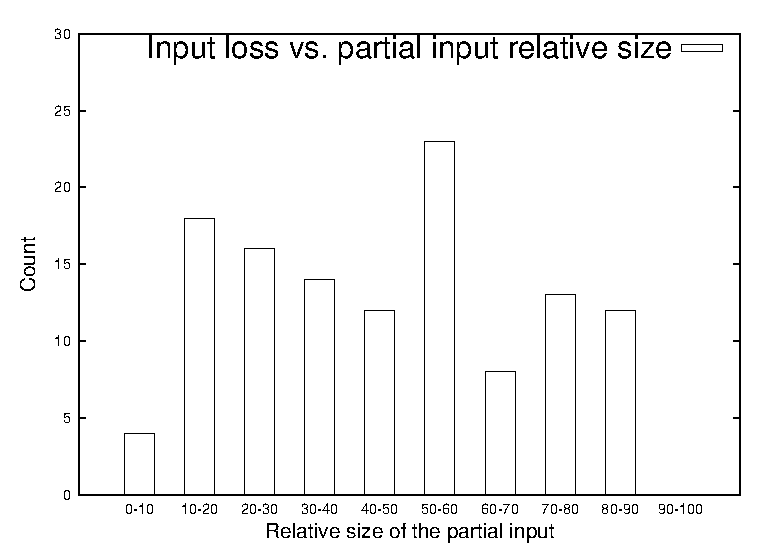
\includegraphics[scale = 0.6]{figures/whenLostInput/Tune.text.nw.v3x08.1stpass.10best.exp.allrules.mmap.nbest1000.1.whenlostinput.eps}
\end{minipage} 
\hfill
\begin{minipage}{.45\textwidth}
  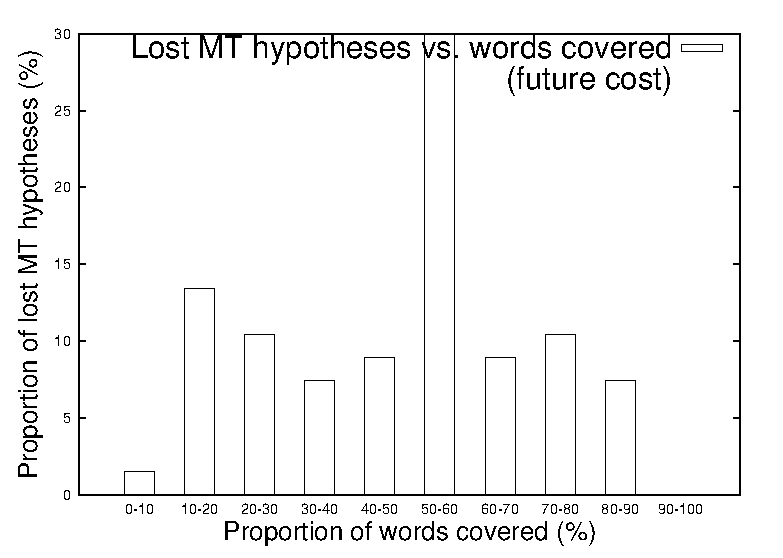
\includegraphics[scale = 0.6]{figures/whenLostInput/Tune.text.nw.v3x08.1stpass.10best.exp.allrules.mmap.nbest1000.1.futurecost.whenlostinput.eps}
\end{minipage}
\caption{Analysis of when the MT hypothesis is lost. The x-axis represents bins of 10\% for the relative size of the input bag-of-word.
The y-axis is simply the count of instances. Future cost estimates are used in decoding for the right hand side figure.}
\label{fig:whenLostInput}
\end{center}
\end{figure}
%
In the next two sections, we will describe two ways of incorporating
information from the translation system in order to at least
match the quality of the translation system.

\section{Regenerate the input with biased lm}
\label{sec:gyroTransBiasedLm}

We have shown in the previous section, that the MT hypothesis, which
we know to be of relatively high quality, is often not regenerated.
In this section, we describe a first solution to remedy this issue.

Our solution is to bias the language model towards the MT hypothesis.
In order to do this, we compute $n$-gram posteriors from the
1st-pass translation lattices~\citep{blackwood:2010:PHD}.
We then convert the posteriors
to integer counts and estimate a
Good-Turing~\citep{good:1953:biometrika,chen-goodman:1998:harvard} smoothed 4-gram
language model from these counts.
We then interpolate this language model with the original language model with
various interpolation parameters.
We obtain the results in \autoref{tab:gyroBiasedLm}.
%
\begin{table}
  \begin{center}
    \begin{tabular}{l|l}
      Config      & Tune BLEU \\
      \hline
      MT Baseline (1st pass) & 34.96 \\
      \hline
      1st-best      & 33.37 \\
      \hline
      1st-best 0.4  & 34.96 \\
      1st-best 0.5  & 34.96 \\
      1st-best 0.6  & 34.96 \\
      1st-best 0.7  & 34.97 \\
      1st-best 0.8  & 34.94 \\
      1st-best 0.9  & 34.90 \\
      1st-best 0.95 & 34.81 \\
      1st-best 0.99 & 34.11 \\
    \end{tabular}
    \caption{Regenerating the MT 1st-best with a biased language model.
      The interpolation parameter is the interpolation weight of the
      original language model.}
    \label{tab:gyroBiasedLm}
  \end{center}
\end{table}
%
We can see that we are able to obtain hypotheses that have
the same quality as the MT hypotheses, and for an interpolation
weight of 0.7, we obtain a very slight improvement on the tuning
set.
We obtain very similar results when we include future cost estimates.
We use the best interpolation weight of 0.7 to run
our regeneration decoder on the test set MT08 and obtain results
in \autoref{tab:gyroBiasedLmTest}.
We obtain slight gains in terms of BLEU score on the MT08 test
using this technique.
%
\begin{table}
  \begin{center}
    \begin{tabular}{l|l|l}
      Config & Tune BLEU & MT08 BLEU \\
      \hline
      MT Baseline (1st pass) & 34.96 & 35.71 \\
      \hline
      1st-best Interpolation 0.7 & 34.97 & 35.75 \\
      1st-best Interpolation 0.7 Future Cost & 34.96 & 35.75 \\
    \end{tabular}
    \caption{Effect of using a language model biased towards
    translation posteriors.}
    \label{tab:gyroBiasedLmTest}
  \end{center}
\end{table}

% TODO maybe redo with less pruning ??

%biased lm union
%\begin{table}
%  \begin{center}
%    \begin{tabular}{l|l|l}
%      Config      & BLEU & Oracle BLEU \\
%      MT Baseline & 34.96 & 56.12 \\
%      union       & 0.3285 & 43.96 \\
%      union 0.4   & TODO
%      union 0.5
%      union 0.6
%      union 0.7
%      union 0.8
%      union 0.9
%      union 0.95
%      union 0.99
%    \end{tabular}
%    \caption{TODO caption}
%  \end{center}
%\end{table}

%biased lm future cost
%\begin{table}
%  \begin{center}
%    \begin{tabular}{l|l|l|l}
%      Config      & BLEU & Oracle BLEU & MT08 \\
%      MT Baseline & 34.96 & 56.12 & 35.71  \\
%      1-best      & 33.40 & 39.18 & 32.79 \\
%      1-best 0.4  & 34.95 & & \\
%      1-best 0.5  & 34.96 &  & \\
%      1-best 0.6  & 34.96 &  & \\
%      1-best 0.7  & 34.96 & & 0.3575 YAY! \\
%      1-best 0.8  & 34.94 & & \\
%      1-best 0.9  & 34.90 & & \\
%      1-best 0.95 & 34.81 & & \\
%      1-best 0.99 & 34.13 & & \\
%    \end{tabular}
%    \caption{TODO caption}
%  \end{center}
%\end{table}

\section{Hypothesis Combination}
\label{sec:gyroTransSysComb}

In the previous section, we have described one way
to obtain hypotheses of comparable quality to the
MT hypotheses. In this section, we present some
hypothesis combination results.
Our hypothesis combination technique
is described in \autoref{sec:lmbr} and is
based on lattice Minimum Bayes' Risk
decoding~\citep{blackwood:2010:PHD}.

Results are presented in \autoref{tab:gyroTransSysComb}.
We can observe that using the union of lattices produced
by NgramGen is beneficial for hypothesis combination.
Using the biased language model described in the
previous section, we are able to match and obtain
a very slight gain over the LMBR rescored translation
hypotheses.
%TODO add row numbers
% TODO describe how gyro is 5g rescored before combination
\begin{table}
  \begin{center}
    \begin{tabular}{l|l|l}
      Config & Tune BLEU & MT08 BLEU \\
      \hline
      MT Baseline (LMBR) & 36.80 & 37.59 \\
      \hline
      NgramGen 1-best Baseline &  36.81 & 37.29 \\
      NgramGen union Baseline & 36.81 & 37.50 \\
      \hline
      NgramGen 1-best Baseline Future Cost & 36.82 & 37.45 \\
      NgramGen union Baseline Future Cost & 36.81 & 37.50 \\
      \hline
      NgramGen 1-best Interp 0.7 & 36.82 & 37.39 \\
      NgramGen union Interp 0.7 & 36.78 & 37.59 \\
      \hline
      NgramGen 1-best Interp 0.7 Future Cost & 36.81 & 37.39 \\
      NgramGen union Interp 0.7 Future Cost & 36.77 & 37.60 \\
    \end{tabular}
    \caption{Hypothesis combination between the output of the translation
    decoder and the output of the regeneration decoder.}
    \label{tab:gyroTransSysComb}
  \end{center}
\end{table}

%\section{Exploiting Confidence Regions}
%\label{sec:gyroTransConfidenceRegions}

%\begin{table}
%  \begin{center}
%    \begin{tabular}{l|l|l}
%      Config & Tune & MT08 \\
%      MT Baseline & 34.96 & 35.71 \\
%      Gyro Baseline & 33.37 & 32.78 \\
%      beta 0.3 & 32.93 &  \\
%      beta 0.4 & 32.94 & \\
%    \end{tabular}
%    \caption{TODO caption}
%  \end{center}
%\end{table}

\section{Conclusion}

In this chapter, we have shown how to apply our regeneration
decoder to the output of a translation system in a 10-best hypothesis
rescoring setting. Because the regeneration decoder only uses
a language model as single feature and throws away ordering
information obtained from the translation system, by simply
running NgramGen on the output of the translation system, translation
performance is degraded.

We have shown two possible ways of integrating the information from the
translation system into the regeneration system in order to match
and slightly outperform the translation quality obtained by the
translation system. The first solution is to bias the language
model used in regeneration towards the MT hypotheses. The second
solution simply takes advantage of well known hypothesis combination
techniques.

%\begin{itemize}
%  \item Experiment with bag of word made of 1-best translation. Show oracle scores. OK
%  \item Experiment with bag of word made of 1-best to 10-best translation. Show oracle scores. OK
%  \item Error analysis: show how often at what stage the input is lost. Conclusion: the
%    decoder needs to be biased towards the input. OK when lost input OK
%  \item Experiments on biasing the decoder towards the input: build language models
%    based on the MT output or based on the MT posteriors. OK
%  \item System combination experiments. OK
%  \item MAYBE: Syntactic n-grams experiments: use the syntactic n-grams to enrich the
%    bag of words and use the dependencies in conjunction with the dependency LM.
%  \item Use gyro together with confidence regions: the confidence regions can be used
%    for chopping and constraints. RUNS
%  \item MAYBE: Use gyro together with position specific posteriors (TBA).
%\end{itemize}

% conclusion
\chapter{Summary and Future Work}

% TODONEVER maybe link to specific experiments on blue in each experimental sections

Statistical Machine Translation was originally framed as a source-channel
model with two main components, the translation model and the
language model. This separation into two modules provided opportunities
for improving each module individually, with the hope that improving the language model
would improve fluency while improving the translation model would improve
adequacy. Current state-of-the-art SMT systems include many more components
that interact in complex ways but also provide further individual improvement
opportunities.

In this thesis, we present various improvements and analyses in the
SMT pipeline, with an emphasis on refining hierarchical phrase-based
models. In \autoref{sec:reviewOfWork}, we review the contributions of
this thesis and in \autoref{sec:thesisFutureWork}, we propose
possible future work for each our contributions.

\section{Review of Work}
\label{sec:reviewOfWork}

This thesis demonstrated various refinements in
hierarchical phrase-based translation systems.
A scalable infrastructure was developed for generating
and retrieving rules from hierarchical grammars. We also
developed an original training method for hierarchical
phrase-based models which leverages computationally
efficient HMM models usually used for word
alignment. Other SMT pipeline components
were refined: we studied the effect of additional
grammar features for domain adaptation and provided recommendations
for language models to be used in first-pass decoding and rescoring.
Finally, we developed a string regeneration system from the
ground up, analysed its competitive performance in
the string regeneration task and its potential application to
rescoring machine translation output. We now review each of
these contributions.

\subsection{Hierarchical Phrase-Based Grammars: Infrastructure}

In order to enable more rapid experimentation and to ensure
scalability for hierarchical phrase-based grammar extraction
and retrieval, we developed a flexible MapReduce implementation
of the grammar extraction and estimation
algorithm~\citep{dyer-cordova-mont-lin:2008:WMT}.
Our implementation described in \autoref{chap:hfile} includes
extensions for the computation
of provenance
features~\citep{chiang-deneefe-pust:2011:ACL} and arbitrary
corpus-level features can be added very easily to our framework.

A framework relying on the HFile format
for efficient retrieval of hierarchical rules to
be used in test set decoding was also developed.
Comprehensive time and memory measurements demonstrated
that our system is competitive with respect to linearly
scanning, possibly concurrently, the datastructure containing
the grammar extracted from parallel
text~\citep{pino-waite-byrne:2012:PBML}.

\subsection{Hierarchical Phrase-Based Grammars: Modelling}

In the SMT pipeline, the word alignment module and
the grammar extraction and estimation module usually
interact through a fixed set of alignment links
produced by the word alignment models. Our contribution
was to allow for more communication between these two
modules~\citep{degispert-pino-byrne:2010:EMNLP}.
In \autoref{chap:extractionFromPosteriors}, we
first reframed the rule extraction procedure
into a general framework. Under this framework, we
introduced two novel methods for grammar extraction
and estimation based on word alignment posterior
probabilities.

The link posterior extraction method was based on alignment
link posterior probabilities and allowed to extract
a greater number of rules more reliably. The phrase pair
posterior method was based on phrase pair alignment posterior
probabilities and was shown to provide a better estimated
translation model. Both methods provided substantial gains in
translation quality in
a medium size Chinese-English translation task.
Alternative strategies for combining source-to-target
and target-to-source word alignment models were also
investigated; hypothesis combination obtained the best
performance in our experiments.

\subsection{Hierarchical Phrase-Based System Development}

The translation model, refined in \autoref{chap:extractionFromPosteriors},
is one of the main features in the log-linear model for translation.
In \autoref{chap:wmt}, we studied the effect of provenance
features~\citep{chiang-deneefe-pust:2011:ACL} for domain adaptation.
The concept of provenance feature was extended from provenance lexical translation
features to provenance translation features. We demonstrated that,
when rule filtering thresholds are applied for each provenance and all
surviving rules are kept, translation gains can be obtained.

We also provided recommendations for language modelling both
in first-pass translation and rescoring. In the context of
domain adaptation, we found that the best strategy for language modelling
was off-line linear interpolation of various language models with
weights tuned for perplexity on a held-out development set as opposed
to log-linear interpolation with weights tuned by MERT.
We also observed that when a few billion words of monolingual data were
available, a two-pass strategy of first-pass decoding with a 4-gram
language model trained on all data followed by 5-gram rescoring
provided the best performance in our experiments.
Finally we confirmed in the rescoring setting previous
observations~\citep{brants-popat-xu-och-dean:2007:EMNLP-CoNLL} in
the first-pass decoding setting
that Kneser-Ney smoothing produced better translation quality than
Stupid Backoff smoothing. Thus we obtained translation quality gains
over the top ranking system in the WMT13 Russian-English
task~\citep{pino-waite-xiao-degispert-flego-byrne:2013:WMT}.

\subsection{Fluency in Hierarchical Phrase-Based Systems}

One main reason for the lack of fluency in machine translation
output is a discrepancy in word order between distant language pairs
such as Chinese and English. In \autoref{chap:gyro}, we
studied the problem of word ordering in isolation through
the string regeneration task. We described a regeneration
model inspired from the phrase-based translation model. We also
built a regeneration decoder
analogous to a stack-based decoder for translation.
We achieved state-of-the-art performance on the string regeneration
task. Finally, we analysed various capabilities of the decoder.

In \autoref{chap:gyroTrans}, we applied string regeneration
to the output of a translation system in a 10-best rescoring setting.
Performance was degraded, however, by combining information obtained
from the translation system with the regeneration system, we were
able to match the quality of the translation output.

\section{Future Work}
\label{sec:thesisFutureWork}

%hfile:
%sentence specific grammar
%parallelize by source sentence
%parallelize by query
%generate source pattern instances more quickly
% real time at the sentence level

The retrieval framework presented in \autoref{chap:hfile}
can exploit parallelisation in two ways for further
speed improvements. First, source pattern instances
can be generated for each test set source sentence individually; then
each source sentence can processed in parallel. Because
the HFile format does not allow multithreaded reads, % TODOFINAL check this on the newest versions
one way to implement this solution is to reuse the multiprocessing
capability of the MapReduce framework.
Another opportunity for parallelisation similar to the one just described
is to process queries in parallel. Again, care has to be taken to use
a multiprocessing approach rather than a multithreading approach.
Finally, the source pattern instance creation step can be fine-tuned
in order to approach the speed of a real time system at the sentence
level.

%posteriors:
%source constraints
%alignment constraints
%target constraints
%ranking function
%counting function
%for all these, explore other models than HMM

In \autoref{chap:extractionFromPosteriors}, the rule extraction
algorithm was described in a framework involving
source constraints, alignment constraints, target constraints, a ranking
function and a counting function. This provides an opportunity
for future work by investigating alternatives to the definitions
of these constraints and ranking and counting functions.
Specifically, other word alignment models may be explored.

% system development
% scale up 5-gram language model data

In \autoref{chap:wmt}, we recommended to use a two-pass
decoding strategy and we also concluded that Kneser-Ney
smoothing was beneficial over Stupid Backoff smoothing
in 5-gram language model rescoring. These recommendations
are valid for language models built on a few billion words.
In the future, we will revise them with language models
trained on an order of magnitude more monolingual data.

% string regeneration
% investigate the use of overlap and use no unigrams
% investigate more features

We successfully applied phrase-based models and decoding
techniques to the task of string regeneration
in \autoref{chap:gyro}. However, interesting future work may
be carried out to investigate the effect of using more features
than simply a language model. In addition, we may study
how overlapping rules can be used to obtain more chances
of covering the entire input if no unigram rules are used.

The effect of additional features for the regeneration
decoder may also be studied in the regeneration of
translation output setting. If translation quality
as measured BLEU does not increase, efforts will be
dedicated to improve fluency while maintaining translation
quality. Finally, more sophisticated future cost estimates
may be studied, such as $n$-gram language model with $n > 1$: this
is possible because when regenerating translation output, the word
ordering information is legitimately available in the input.

% string regeneration for translation
% fluency
% more features
% TODONEVER mention dependency language model


\bibliographystyle{plainnat}
\bibliography{thesis}

\end{document}
